\documentclass[11pt]{report}
\usepackage{makeidx}
\usepackage{graphics}
\usepackage{amssymb}
\pagestyle{headings}
\makeindex
\parindent=0mm
%\textwidth=6.0in
%\textheight=8.0in
%\oddsidemargin=-.35i
%\evensidemargin=-.35in
%\topmargin=-.50in

\newtheorem{thr}{Theorem}
%\font\bb=msym10
\def\N{{\Bbb N}}
\def\Z{{\Bbb Z}}
\def\R{{\Bbb R}}
%
% macros pour les diagrammes rectangulaires
%
\def\hfl#1#2{\smash{\mathop{\hbox to 15mm{\rightarrowfill}}
\limits^{\scriptstyle#1}_{\scriptstyle#2}}}
%
\def\hflr#1#2{\smash{\mathop{\hbox to 15mm{\rightarrowfill}}
\limits^{\scriptstyle#1}_{\scriptstyle#2}}}
%
\def\hfll#1#2{\smash{\mathop{\hbox to 15mm{\leftarrowfill}}
\limits^{\scriptstyle#1}_{\scriptstyle#2}}}
%
\def\vfl#1#2{\llap{$\scriptstyle #1$}\left\downarrow
\vbox to 7mm{}\right.\rlap{$\scriptstyle #2$}}
%
\def\vflu#1#2{\llap{$\scriptstyle #1$}\left\uparrow
\vbox to 7mm{}\right.\rlap{$\scriptstyle #2$}}
%
\def\diagram#1{\def\normalbaselines{\baselineskip=0pt
\lineskip=10pt\lineskiplimit=1pt} \matrix{#1}}
%
% macro tvi pour les lignes verticales et horizontales dans un tableau
%
\def\tvi{\vrule height 12pt depth 5pt width 0pt}
\def\tv{\tvi\vrule}

\begin{document}
\pagenumbering{roman}
\begin{titlepage}
\   \\ \\ \\ \\ \\ \\ \\ \\ \\ \\ \\ 
\begin{center}
 {\huge KENZO} \\ 
\    \\
 {\Large a Symbolic Software} \\
  for \\
 {\Large  Effective Homology Computation} 
\vskip 0.5cm
-----
\vskip 0.5cm
Julio Rubio Garcia\\
Francis Sergeraert \\
Yvon Siret
\vskip 0.20cm
-----
\vskip 0.20cm
Institut Fourier \\
Grenoble, France \\
\vskip 0.20cm
-----
\vskip 0.20cm
\end{center}
\vskip 0.5cm
This document is a user guide for the 
basic modules of the Effective Ho\-mo\-lo\-gy Software (Kenzo Version 1998). \\
It is also available by anonymous ftp ({\bf ftp fourier.ujf-grenoble.fr})
in the directory {\bf /pub/KENZO}. \\
\vskip 0.5cm
\begin{center}
{\em \today} \\
\end{center}
\end{titlepage}
\vskip 1in
\centerline {FOREWORD}
\vskip 0.5in
   The {\bf Kenzo}  program implements the general  ideas of  the second author
about \emph{Effective Homology}\footnote{{\bf Francis Sergeraert.}
\emph{The computability problem in algebraic topology}.
Advances in Mathematics, 1994, vol. 104, pp 1-29.},
mainly around the Serre and Eilenberg--Moore spectral sequences.
The first author (re--) discovered the importance
of the  \emph{Basic  Perturbation Lemma}  in these  questions, already
noted by  Victor  Gugenheim\footnote{{\bf V.K.A.M. Gugenheim.}
\emph{On a perturbation theory for the homology of the loop space}.
Journal of Pure and Applied Algebra, 1982, vol. 25, pp 197-205.}
and this  program  directly
implements and  directly uses this ``lemma''  which should be called the
\emph{Fundamental Theorem of   Algebraic  Topology}. The first version of the program, 
called {\bf EAT}, was written in  1989-90 by the  first and the second authors.
It  has been demonstrated in  several universities: France: Grenoble and
Montpellier, Belgium:  Louvain-la-Neuve, Italy: Genoa and Pisa, 
Sweden: Stockolm, Japan:
Sapporo, Morioka, Urawa, Tokyo,  Kyoto, Nara, Osaka and Hiroshima. 
\par
In this {\bf Kenzo} version, numerous improvements have been integrated in comparison with
{\bf EAT}.
\begin{enumerate}
\item Standard CLOS (Common Lisp Object System) techniques.
\item Use of the Zermelo theorem about ordered sets (!): any set can be
well ordered and this remark gives important new ideas to improve
execution speed.
\item Better memory management.
\item Use of Szczarba's formulas instead of Shih's for implementing the twisted
Eilenberg--Zilber theorem.
\item New mathematical objects:
\begin{itemize}
\item Serre spectral sequences.
\item Differentials algebras.
\item Simplicial morphisms.
\item Kan simplicial sets.
\item Simplicial groups.
\item Fibrations.
\item Classifying spaces.
\end{itemize}
In particular, using these tools, the first homotopy groups of {\em arbitrary} 
simplicial sets with effective homology, are now reachable.
\end{enumerate}
\par
The present documentation is a joint work between the second and third authors.
\cleardoublepage
\setcounter{chapter}{-1}
\chapter {Overview}

In this overview we try to  show, without entering in detailed
explanations, various possibilities of {\tt Kenzo} in algebraic topology.
The lines ended by the symbol $==>$ are the commands typed by the user 
(don't type this symbol!).
They are followed by the answer of the program. We have suppressed some
extra informations, in particular the ones printed during the computation
of homology groups.
\vskip 0.5cm
Let us begin by the space $Moore({\Z}/2{\Z}, 3)$ described as a simplicial set
having only three non--degenerate simplices, namely in dimension
$0$, $3$ and $4$. In the  representation created by the software, the $0$--simplex (base point),
the $3$--simplex and the $4$--simplex are respectively labelled
``{\tt *}'', {\tt M3} and {\tt N4}. Two faces of the $4$-simplex {\tt N4} are identified with the
$3$-simplex {\tt M3}, the others being contracted on the base point. To create the simplicial set
one types simply:
{\footnotesize\begin{verbatim}
(setf m23 (moore 2 3))  ==>
\end{verbatim}}
The system answers that a {\tt Kenzo} object has been created, with number $1$ and
type {\tt SIMPLICIAL SET}. This object may be referenced  by the symbol {\tt m23}.
{\footnotesize\begin{verbatim}
[K1 Simplicial-Set]
\end{verbatim}}
We may compute the homology groups of this space, using the underlying chain complex
induced by the simplicial set description. Here we compute the $ H_i$ from $0$ to $4$ included.
When in the answer the component part is void, it means that the corresponding homology group is null.
{\footnotesize\begin{verbatim}
(homology m23 0 5)  ==>

Homology in dimension 0 :

Component Z

--done--

Homology in dimension 1 :

--done--

Homology in dimension 2 :

--done--

Homology in dimension 3 :

Component Z/2Z

--done--

Homology in dimension 4 :

---done---
\end{verbatim}}
As {\tt m23} is a simplicial set, it is possible to create the cartesian product
$m23 \times m23$ by the function {\tt crts-prdc}. This is a new simplicial set.
{\footnotesize\begin{verbatim}
(setf m23xm23 (crts-prdc m23 m23))  ==>

[K10 Simplicial-Set]
\end{verbatim}}
Being a simplicial set, {\tt m23xm23} is also a chain complex object and we may for instance ask for
the basis in dimension $6$
{\footnotesize\begin{verbatim}
(basis m23xm23 6)  ==>

(<CrPr 1-0 N4 3-2 N4> <CrPr 1-0 N4 4-2 N4> <CrPr 1-0 N4 4-3 N4> 
 <CrPr 1-0 N4 4-3-2 M3>  <CrPr 1-0 N4 5-2 N4> <CrPr 1-0 N4 5-3 N4> 
 <CrPr 1-0 N4 5-3-2 M3> <CrPr 1-0 N4 5-4 N4>
                            ....  .... 
 <CrPr 4-1 N4 5-3-2 M3> <CrPr 4-1-0 M3 3-2 N4> <CrPr 4-1-0 M3 5-2 N4> 
 <CrPr 4-1-0 M3 5-3 N4> <CrPr 4-1-0 M3 5-3-2 M3> ... ... ...)

(length *)  ==>        

230
\end{verbatim}}
As shown by the last command (* means the previous result), 
the number of elements of the basis is quite large (230). The user
will note that the basis elements are formed by cartesian products of {\em degenerated simplices}. In
the list, an element like {\tt <CrPr 1-0 N4 5-3-2 M3>} means $\eta_1\eta_0 N4 \times \eta_5\eta_3\eta_2 M3$.
\par
We may construct also the tensor product $m23 \otimes m23$ from the underlying chain complex
of the simplicial set {\tt m23}. This tensor product is a new chain complex and we see that the
basis in dimension $6$ has only one element:
{\footnotesize\begin{verbatim}
(setf t2m23 (tnsr-prdc m23 m23)) ==>

[K3 Chain-Complex]

(basis t2m23 6)  ==>

(<TnPr M3 M3>)
\end{verbatim}}
The Eilenberg-Zilber theorem is used to compute the homology groups of the cartesian
product space: as chain complexes, {\tt m23xm23} and {\tt t2m23} have the same homology groups,
but the computations using the tensor product are considerably faster.
{\footnotesize\begin{verbatim}
(homology m23xm23 0 8)  ==>

Homology in dimension 0 :

Component Z

Homology in dimension 1 :    (meaning: Group null)

Homology in dimension 2 :

Homology in dimension 3 :

Component Z/2Z

Component Z/2Z

Homology in dimension 4 :

Homology in dimension 5 :

Homology in dimension 6 :

Component Z/2Z

Homology in dimension 7 :

Component Z/2Z

---done---
\end{verbatim}}
\newpage
Let us consider now the space $K({\Z}, 1)$. This is an Abelian simplicial group created  in {\tt Kenzo} 
by the function {\tt k-z}.
In this simplicial group, a  simplex  in dimension $n$ 
is mathematically represented by a sequence of integers, known as a {\em bar} object:
$$ [a_1 \mid a_2 \mid \ldots \mid a_n]. $$
In {\tt Kenzo}, a non-degenerate simplex of $K({\Z},1)$ in dimension $n$ will be simply 
a list of $n$ non-null integers, for instance: {\tt (2 3 4 5)}. In dimension $0$, the only
simplex is {\tt NIL} (the base point).
{\footnotesize\begin{verbatim}
(setf kz1 (k-z 1))  ==>

[K38 Abelian-Simplicial-Group]
\end{verbatim}}
But this object is also a {\em coalgebra} and an {\em algebra}, and we may
see the effect of the respective induced {\em coproduct} and {\em product}:
{\footnotesize\begin{verbatim}
(cprd kz1 4 '(2 3 4 5))  ==>

----------------------------------------------------------------------{CMBN 4}
<1 * <TnPr NIL (2 3 4 5)>>
<1 * <TnPr (2) (3 4 5)>>
<1 * <TnPr (2 3) (4 5)>>
<1 * <TnPr (2 3 4) (5)>>
<1 * <TnPr (2 3 4 5) NIL>>
------------------------------------------------------------------------------

(aprd kz1 6 (tnpr 2 '(1 2) 4 '(3 4 5 6)))  ==>

----------------------------------------------------------------------{CMBN 6}
<1 * (1 2 3 4 5 6)>
<-1 * (1 3 2 4 5 6)>
<1 * (1 3 4 2 5 6)>
<-1 * (1 3 4 5 2 6)>
<1 * (1 3 4 5 6 2)>
<1 * (3 1 2 4 5 6)>
<-1 * (3 1 4 2 5 6)>
<1 * (3 1 4 5 2 6)>
<-1 * (3 1 4 5 6 2)>
<1 * (3 4 1 2 5 6)>
<-1 * (3 4 1 5 2 6)>
<1 * (3 4 1 5 6 2)>
<1 * (3 4 5 1 2 6)>
<-1 * (3 4 5 1 6 2)>
<1 * (3 4 5 6 1 2)>
------------------------------------------------------------------------------
\end{verbatim}}
The printed results are the printed representation of {\em combinations}, i.e.
integer linear combinations of generators resulting from the application of the
morphisms. The degree of the combination is indicated by the information: {\tt CMBN $n$}.
\par
On the same way, we may create the Abelian simplicial groups $K({\Z}/2{\Z}, n)$:
{\footnotesize\begin{verbatim}
(setf k-z2-2 (k-z2 2))  ==>

[K488 Abelian-Simplicial-Group]

(homology k-z2-2 4)  ==>

Homology in dimension 4 :

Component Z/4Z

---done---
\end{verbatim}}

\begin{center}
----------
\end{center}
Let us play now with the sphere $S^3$ and its loop spaces. $S^3$ and $\Omega^2 S^3$ are created by
respective calls to the functions {\tt sphere} and {\tt loop-space}. Then we compute the $H_4$ and $H_5$
of $\Omega^2 S^3$:
{\footnotesize\begin{verbatim}
(setf s3 (sphere 3))  ==>

[K52 Simplicial-Set]

(setf o2s3 (loop-space s3 2))  ==>

[K69 Simplicial-Group]

(homology o2s3 4 6)  ==>

Homology in dimension 4 :

Component Z/3Z

Component Z/2Z

Homology in dimension 5 :

Component Z/3Z

Component Z/2Z

---done---
\end{verbatim}}
\newpage
Let us take now the first loop space $\Omega^1 S^3$ 
{\footnotesize\begin{verbatim}
(setf s3 (sphere 3))  ==>

[K94 Simplicial-Set]

(setf os3 (loop-space s3))  ==>

[K99 Simplicial-Group]
\end{verbatim}}
In the following instruction, we locate in the symbol {\tt L1} the canonical generator of 
$\pi_2 (\Omega^1S^3)$, that is the $2$--simplex coming from the original sphere. In fact, the object
created by the command {\tt (loop3 0 's3 1)} is the ``word'' $S3^1$ belonging to the 
Kan simplicial version $G(S^3)$ (a simplicial group) of the loop space $\Omega S^3$. 
{\footnotesize\begin{verbatim}
(setf L1  (loop3 0 's3 1))  ==>

<AbSm - <<Loop[S3]>>>
\end{verbatim}}
Let us consider also the $2$--degeneracy of the base point of the loop space. In the printed
result, the user will recognize the degeneracy $\eta_1\eta_0$ of the null loop, base point of
$\Omega^1 S^3$:
{\footnotesize\begin{verbatim}
(setf null-simp (absm 3 +null-loop+))  ==>

<AbSm 1-0 <<Loop>>>
\end{verbatim}}
We may  build now a new space by pasting a disk $D3$ as indicated by the 
following call. It means that we ``paste'' to the space {\tt os3} a $3$--simplex named {\tt D3},
the attaching map being described by the list of its faces in dimension $2$.

{\footnotesize\begin{verbatim}
(setf dos3 (disk-pasting os3 3 '<D3> 
              (list L1 null-simp L1 null-simp)))  ==>

[K212 Simplicial-Set]
\end{verbatim}}
Let us compute a few homology groups of the new space {\tt dos3}:
{\footnotesize\begin{verbatim}
(homology dos3 2 4)  ==>

Homology in dimension 2 :

Component Z/2Z

Homology in dimension 3 :

---done---
\end{verbatim}}
But more interesting, let us  build the  loop space of the object {\tt dos3} and 
let us compute  the ho\-mo\-lo\-gy in dimension $5$:
{\footnotesize\begin{verbatim}
(setf odos3 (loop-space dos3))  ==>

[K230 Simplicial-Group]

(homology odos3 5)  ==>

Homology in dimension 5 :

Component Z/2Z

Component Z/2Z

Component Z/2Z

Component Z/2Z

Component Z/2Z

Component Z/2Z

Component Z

--done--
\end{verbatim}}
\begin{center}
--------
\end{center}
Let us continue with the Kan theory. First, we check that $S^3$ is not of type Kan and that $\Omega S^3$
is indeed of type Kan and a non--Abelian simplicial group.
{\footnotesize\begin{verbatim}
(typep s3 'kan)  ==>

NIL

(typep os3 'kan)  ==>

T

(typep os3 'simplicial-group)  ==>

T

(typep os3 'ab-simplicial-group)  ==>

NIL


\end{verbatim}}
Let us create the word $L2=(S3)^2$, i.e an object belonging to $\Omega S^3$ and let us
apply the product of the underlying algebra upon $L2 \otimes L2$:
{\footnotesize\begin{verbatim}
(setf L2 (loop3 0 's3 2))  ==>

<<Loop[S3\2]>>

(setf square (aprd os3 4 (tnpr 2 L2 2 L2)))  ==>

----------------------------------------------------------------------{CMBN 4}
<1 * <<Loop[1-0 S3\2][3-2 S3\2]>>>
<-1 * <<Loop[2-0 S3\2][3-1 S3\2]>>>       <-------
<1 * <<Loop[2-1 S3\2][3-0 S3\2]>>>
<1 * <<Loop[3-0 S3\2][2-1 S3\2]>>>
<-1 * <<Loop[3-1 S3\2][2-0 S3\2]>>>
<1 * <<Loop[3-2 S3\2][1-0 S3\2]>>>
------------------------------------------------------------------------------
\end{verbatim}}
We see that the result is a linear combination of words composed from degeneracies
of {\tt L2}. The following instruction selects the generator part of the
second element of the previous combination (noted by the reverse arrow).
{\footnotesize\begin{verbatim}
(setf L4 (gnrt (second (cmbn-list square))))  ==>

<<Loop[2-0 S3\2][3-1 S3\2]>>
\end{verbatim}}
Let us use the lisp function {\tt mapcar} (one among the various iteration functions of Lisp) to
create the list of the faces 1, 2, 3 and 4 of the object {\tt L4}, this list is a ``Kan hat''.
{\footnotesize\begin{verbatim}
(setf hat (mapcar #'(lambda (i) (face os3 i 4 l4)) '(1 2 3 4)))  ==>

(<AbSm - <<Loop[1 S3\2][2 S3\2]>>> <AbSm - <<Loop[0 S3\2][2 S3\2]>>> 
 <AbSm - <<Loop[0 S3\2][1 S3\2]>>> <AbSm 1 <<Loop[S3\2]>>>)
\end{verbatim}}
The function {\tt kfll} tries to find a filling of this ``Kan hat'', and we see that 
the face $2$ of the resulting simplex (which is very different from {\tt L4}) is  the same 
as the face $2$ of {\tt L4}.
{\footnotesize\begin{verbatim}
(setf kan-simplex (kfll os3 0 4 hat))  ==>

<AbSm - <<Loop[3-1 S3\2][2-1 S3\-2][2-0 S3\2][1-0 S3\-2][2-1 S3\2][3-1 S3\-2]
              [1-0 S3\2][3-1 S3\2][3-0 S3\-2][1-0 S3\-2][3-0 S3\2][2-0 S3\-2]
              [1-0 S3\2][3-0 S3\-2][2-0 S3\2][3-0 S3\2]>>>

(face os3 2 4 kan-simplex)  ==>

<AbSm - <<Loop[0 S3\2][2 S3\2]>>>

(second hat)  ==>

<AbSm - <<Loop[0 S3\2][2 S3\2]>>>
\end{verbatim}}
\begin{center}
--------
\end{center}
Let ${\cal G}$ be a simplicial group $0$--reduced. $\Omega S^3$ is such a group.
The software  {\tt Kenzo} allows 
the construction of the universal bundle $\bar{\cal W}{\cal G}$, i.e. the 
classifying space of ${\cal G}$. In our case, as $\Omega S^3$ in non--Abelian, the
result is not a simplicial group but only a simplicial set. We verify that the $H_4$ is null.
{\footnotesize\begin{verbatim}
(setf cls-os3 (classifying-space os3))  ==>

[K598 Simplicial-Set]

(typep cls-os3 'simplicial-group)  ==>

NIL

(homology cls-os3 4)  ==>

Homology in dimension 4 :

---done---
\end{verbatim}}
\begin{center}
--------
\end{center}
\vskip 0.40cm
Let us end this short overview with an example of computation of homotopy groups.
The method used in {\tt Kenzo} is the Whitehead tower. 
In this current version only the case where the first non--null
homology group (in non--null dimension) is ${\Z}$ or ${\Z}/{2 {\Z}}$ can be processed; however if this 
homology group is a direct sum of several copies of ${\Z}$ or ${\Z}/{2 {\Z}}$, then the corresponding
stage of the Whitehead tower may also be constructed step by step.
\vskip 0.40cm
We take again $Moore({\Z}/2{\Z}, 3)$ whose $H_3$ is ${\Z}/2{\Z}$. First the fundamental cohomology
class is constructed:
{\footnotesize\begin{verbatim}
(setf ch3 (chml-clss m23 3))  ==>

[K729 Cohomology-Class on K1 of degree 3]
\end{verbatim}}
Then the function {\tt z2-whitehead} is called to build a fibration over the simplicial set {\tt m23}
canonically associated to the cohomology class {\tt ch3}.
{\footnotesize\begin{verbatim}
(setf f3 (z2-whitehead m23 ch3))  ==>

[K730 Fibration K1 -> K488]
\end{verbatim}}
Then the total space of the fibration is built:
{\footnotesize\begin{verbatim}
(setf x4 (fibration-total f3))  ==>

[K736 Simplicial-Set]
\end{verbatim}}
The $H_4$ of this total space is the $\pi_4$ of $Moore({\Z}/2{\Z})$:
{\footnotesize\begin{verbatim}
(homology x4 3 5)  ==>

Homology in dimension 3 :

---done---

Homology in dimension 4 :

Component Z/2Z

---done---
\end{verbatim}}
We may now iterate the process, to compute the $\pi_5$ of $Moore({\Z}/2{\Z})$:
{\footnotesize\begin{verbatim}
(setf ch4 (chml-clss x4 4))  ==>

[K817 Cohomology-Class on K802 of degree 4]

(setf f4 (z2-whitehead x4 ch4))  ==>

[K832 Fibration K736 -> K818]

(setf x5 (fibration-total f4))  ==>

[K838 Simplicial-Set]

(homology x5 4 6)  ==>

Homology in dimension 4 :

---done---

Homology in dimension 5 :

Component Z/4Z

---done---
\end{verbatim}}
So $\pi_5(Moore({\Z}/2{\Z}))$ is ${\Z}/4{\Z}$.
\tableofcontents
\cleardoublepage
\pagenumbering{arabic}
\chapter{Chain Complexes}

%\pagenumbering{arabic}

\section{Introduction}

A\index{chain complex} {\em chain complex}\footnote{{\bf P.J. Giblin} in 
{\em Graph, Surface and Homology}, Chapman and Hall Math. series, 1981.}
($C_p, d_p$) is a collection of free $\Z$--modules ($C_p$), one for each
$p \in \Z$, together with a homomorphism $d_p : C_p \rightarrow C_{p-1}$, such
that, for all $p$, $d_{p-1} \circ d_p = 0$. 
\par
{\bf In the Kenzo program}, a  {\em  morphism}\index{morphisms! in {\tt Kenzo}} $f=(f_p)$, of degree $k$, 
from a chain complex ($C_p, d_p$) to another ($C'_p, d'_p$) is a
collection of homomorphisms 
$$f_p : C_p \rightarrow C'_{p+k}.$$
This is expressed by the following  diagram, generally {\bf not assumed commutative}.

$$\diagram{
\cdots & \leftarrow & C_{p-1} & \buildrel {d_p} \over \longleftarrow 
                     & C_p     & \buildrel {d_{p+1}} \over \longleftarrow 
                     & C_{p+1} 
       & \leftarrow & \cdots \cr
       &             & \vfl {\displaystyle {f_{p-1}}}{} 
       &             & \vfl {\displaystyle {f_p}}{} 
       &             & \vfl {\displaystyle {f_{p+1}}}{} \cr
\cdots & \leftarrow & C'_{p+k-1} & \buildrel {d'_{p+k}} \over \longleftarrow 
                     & C'_{p+k}     & \buildrel {d'_{p+k+1}} \over \longleftarrow 
                     & C'_{p+k+1} 
       & \leftarrow & \cdots \cr }
$$

\newpage
Three types of   morphisms are most generally considered.
\begin{enumerate}
\item $k=0$. If the commutativity relation $d'_p\circ f_p=f_{p-1}\circ d_p$ holds for every $p$, then the morphism
$f$ is an ordinary chain complex morphism or {\em chain map}\index{chain map}.
\item $k=-1$. If $(C_p,d_p)=(C'_p,d'_p)$ and $f_p=d_p$, then $f$ is the 
{\em differential}\index{chain complex!differential} of the chain complex
$(C_p,d_p)$ and, in fact, this differential is implemented in the {\tt Kenzo} program as a morphism of degree $-1$.
\item $k=+1$. In this case, $f$ is usually a {\em homotopy operator}\index{homotopy operator}, that is, some relation
$$d'_{p+1}\circ f_p+f_{p-1}\circ d_p=g_p-g'_p$$
is satisfied for two (ordinary) chain complex morphisms $g$ and $g'$.
\end{enumerate}
For technical reasons, these three types of morphisms have been implemented in the {\tt Kenzo} program
in a unique type.

\section {Generators, terms and combinations}

To become familiar to the lisp functions implementing the chain complexes, the best is to begin
by an example of chain complex. The {\em simplicial complexes}\index{simplicial complexes} are good candidates
for this purpose and we shall take as typical example the following simplicial
complex.
%
\vskip 0.50cm
\centerline{\psfig{figure=/home/home/siret/Kenzo/diabolo.eps}}
\vskip 0.50cm
%
In this simplicial complex, called here {\em diabolo}, there are $3$ associated chain groups.
\begin{itemize}
\item $C_0$, the free $\Z$--module on the set of vertices $\{s_0,s_1,s_2,s_3,s_4,s_5 \}$.
\item $C_1$, the free $\Z$--module on the set of  edges 
   $\{ s_{01}, s_{02}, s_{12}, s_{23}, s_{34}, s_{35}, s_{45} \}$.
\item $C_2$, the free $\Z$--module on the set of  triangles (here a singleton)
   $\{ s_{345} \}$.
\end{itemize}
The elements of either of those groups $C_p$ are linear integer combinations  of the
corresponding basis\index{chain complex!basis} (set of $\sigma_i$'s), i.e. elements of the form:
$$ \sum {\lambda_i \sigma_i}, \quad \lambda_i \in \Z. $$
An element $\sigma_i$ of any basis is also called {\em generator}\index{generator} and in our specific case
this generator will be represented by a  lisp symbol. For instance,
$s_{45}$ will be translated in {\tt s45}. But, the user must know from now, that in the realistic
usage of the software, generators may be of any type.
A product such as $\lambda_i \sigma_i$ is called
a {\em term}\index{term} and a sum of terms, a {\em combination}\index{combination}.

\subsection {Representation of a combination}

A combination\index{combination!representation} is represented internally in the system by a  list 
having the general following form:
\begin{center}
{\tt (:cmbn {\em degree} $(\lambda_1.\sigma_1)$ ... $(\lambda_k.\sigma_k)$)}
\end{center}
and containing
\begin{enumerate}
\item The degree of the combination  corresponding to the index $p \in \Z$  of the group 
$C_p$ to which this combination belongs.
\item The  list of the internal representation of the terms, namely the list of pairs $(\lambda_i.\sigma_i)$.
\end{enumerate}
This choice of representation implies that only homogeneous combinations
will be considered. A type {\tt CMBN} and 
a printing method have been associated to this internal representation. The external
form of a combination is shown in the  examples. 

\subsection {Ordering the generators}

In order\index{generator!ordering} to speed up the execution of algorithms involving combinations,
the list of pairs $(\lambda_i.\sigma_i)$ is ordered by an adequate ordering function (ex: the  lexicographical ordering
on the symbols). For programming convenience, an enumerated type {\tt CMPR} has been defined:
{\footnotesize\begin{verbatim}
(deftype cmpr() '(member :less :equal :greater))
\end{verbatim}}
A number of macros, functions and methods have been defined
on usual sets (symbols, numbers, lists, ...) taking their value in the set
{\tt [:less, :equal, :greater]}. Of course, the user may define its own function for a particular case.
There exists functions to compare various couples of usual items:
\vskip 0.45cm
{\parindent=0mm
{\leftskip=5mm 
{\tt f-cmpr} {\em n1 n2}\hfill {\em [Function]} \par}
{\leftskip=12mm 
Return {\tt :less}, {\tt :equal}, {\tt :greater}, according to the result of
the canonical comparison of both integers {\em n1} and {\em n2}. \par}
{\leftskip=5mm 
{\tt s-cmpr} {\em symbol1 symbol2} \hfill {\em [Function]}\par}
{\leftskip=12mm 
Return  {\tt :less}, {\tt :equal}, {\tt :greater}, according to the result of
the lisp comparison functions on the strings {\tt (symbol-name {\em symbol1})}
and {\tt (symbol-name {\em symbol2})} \par}
{\leftskip=5mm 
{\tt l-cmpr} {\em list1 list2}\hfill {\em [Function]} \par}
{\leftskip=12mm 
Return  {\tt :less}, {\tt :equal}, {\tt :greater}, according to the 
lexicographical ordering of the two lists  {\em list1}
and {\em list2} representing legal generators in this implementation. \par}
}

\subsection* {Examples}

{\footnotesize\begin{verbatim}
(f-cmpr 123 789)  ==>

:LESS

(s-cmpr 'circulation 'circular)  ==>

:GREATER

(s-cmpr 'qwerty 'qwerty)  ==>

:EQUAL

(l-cmpr '(1 a b) '(1 a))  ==>

:GREATER
\end{verbatim}}
\newpage

\subsection {Functions handling  combinations}

The software provides a set of functions, methods or macros to create or modify 
combinations\index{combination!handling}. 
\vskip 0.45cm
{\parindent=0mm
{\leftskip=5mm 
{\tt term-cmbn} {\em dgr cf gnr} \hfill {\em [Macro]}\par}
{\leftskip=15mm 
Construct the combination of degree {\em dgr} with unique term $cf * gnr$ \par}
{\leftskip=5mm 
{\tt cmbn} {\em dgr cf1 gnr1 cf2 gnr2 ... cfn gnrn}\hfill {\em [Function]} \par}
{\leftskip=15mm 
Construct a combination of degree {\em dgr}, sum of the terms $cf_i *  gnr_i$. The sequence of pairs
$\lbrace cf_i\  gnr_i \rbrace$ has an undefinite length and  may be void. In this case,  the combination
is a null combination of degree {\em dgr}.  \par}
{\leftskip=5mm 
{\tt cmbn-p} {\em object} \hfill {\em [Function]}\par}
{\leftskip=15mm 
Test is {\em object} is a legal combination. \par}
{\leftskip=5mm 
{\tt cmbn-degr} {\em cmbn}   \hfill {\em [Macro]} \par}
{\leftskip=15mm 
Get the degree (an integer) of the combination {\em cmbn}. \par}
{\leftskip=5mm 
{\tt cmbn-list} {\em cmbn}   \hfill {\em [Macro]} \par}
{\leftskip=15mm 
Get the list of the terms  of the combination {\em cmbn}. Beware: a term is not a {\tt Kenzo} object.
One may select the coefficient (an integer) or the generator -- a {\tt Kenzo} object -- 
respectively by the macros {\tt cffc} and {\tt gnrt}. \par}
{\leftskip=5mm 
{\tt zero-cmbn} {\em dgr}   \hfill {\em [Function]} \par}
{\leftskip=15mm 
Create an instance of a null combination in the degree {\em dgr}. \par}
{\leftskip=5mm 
{\tt zero-pure-dffr} {\em cmbn} \hfill {\em [Function]} \par}
{\leftskip=15mm 
Create  a null combination of degree $degr(cmbn) - 1$. \par}
{\leftskip=5mm 
{\tt cmbn-zero-p} {\em cmbn} \hfill {\em [Macro]}\par}
{\leftskip=15mm 
Test if {\em cmbn} is a null combination in any degree. \par}
{\leftskip=5mm 
{\tt cmbn-non-zero-p} {\em cmbn} \hfill {\em [Macro]} \par}
{\leftskip=15mm 
Test if {\em cmbn} is a non-null combination in any degree. \par}
{\leftskip=5mm 
{\tt cmbn-opps} {\em cmbn} \hfill {\em [Function]} \par}
{\leftskip=15mm 
Create a  combination opposite to {\em cmbn}. \par}
{\leftskip=5mm 
{\tt n-cmbn} {\em n cmbn} \hfill {\em [Function]} \par}
{\leftskip=15mm 
Create a  combination multiple of  {\em cmbn} by the factor $n$. \par}
{\leftskip=5mm 
{\tt 2cmbn-add} {\em cmpr cmbn1 cmbn2} \hfill {\em [Function]} \par}
{\leftskip=15mm 
Create a combination, sum of both combinations {\em cmbn1} and {\em cmbn2}. The first
argument, {\em cmpr}, must be a function or macro relevant to compare the generators of the
involved combinations, in order to return an ordered combination. \par}
}
\newpage
{\parindent=0mm
{\leftskip=5mm 
{\tt ncmbn-add} {\em cmpr cmbn1 cmbn2 ... cmbnk} \hfill {\em [Function]} \par}
{\leftskip=15mm 
Create a combination, sum of the indefinite number of combinations $cmbn_i$. As to the first
argument, {\em cmpr}, see the function {\tt 2cmbn-add}. \par}
{\leftskip=5mm 
{\tt 2n-2cmbn} {\em cmpr n1 cmbn1 n2 cmbn2} \hfill {\em [Function]} \par}
{\leftskip=15mm 
Build the combination $n1 * cmbn1 + n2 * cmbn2$. Both integers $n1$ and $n2$ must be
non null. As to the first argument, {\em cmpr}, see the function {\tt 2cmbn-add}. \par}
{\leftskip=5mm 
{\tt 2cmbn-sbtr} {\em cmpr cmbn1 cmbn2} \hfill {\em [Function]} \par}
{\leftskip=15mm 
Create a combination, difference of {\em cmbn1} and {\em cmbn2}. 
As to the first argument, {\em cmpr}, see the function {\tt 2cmbn-add}. \par}
}
\subsection* {Examples}

{\footnotesize\begin{verbatim}
(setf comb1 (cmbn 1 1 'u 2 'v 3 'w 4 'z))  ==>
-----------------------------------------------------------------------{CMB 1}
<1 * U>
<2 * V>
<3 * W>
<4 * Z>
------------------------------------------------------------------------------

(cmbn-non-zero-p comb1)  ==>

T

(cmbn-list comb1)  ==>

((1 . U) (2 . V) (3 . W) (4 . Z))

(setf term3 (third *))  ==>  ;; not a Kenzo object!

(3 . W)

(cffc term3)  ==>

3

(gnrt term3)  ==>

W
\end{verbatim}}
\newpage
{\footnotesize\begin{verbatim}
(setf mcomb1 (cmbn-opps comb1))   ==>

-----------------------------------------------------------------------{CMB 1}
<-1 * U>
<-2 * V>
<-3 * W>
<-4 * Z>
------------------------------------------------------------------------------

(setf comb2 (n-cmbn 10 comb1))  ==>

-----------------------------------------------------------------------{CMB 1}
<10 * U>
<20 * V>
<30 * W>
<40 * Z>
------------------------------------------------------------------------------

(setf cmb12 (2cmbn-add #'s-cmpr comb1 comb2))  ==>

----------------------------------------------------------------------{CMBN 1}
<11 * U>
<22 * V>
<33 * W>
<44 * Z>
------------------------------------------------------------------------------

(2cmbn-sbtr #'s-cmpr comb1 cmb12)  ==>

----------------------------------------------------------------------{CMBN 1}
<-10 * U>
<-20 * V>
<-30 * W>
<-40 * Z>
------------------------------------------------------------------------------

(ncmbn-add #'s-cmpr 
           comb1 comb2 comb1 comb2 comb1 comb2 comb1 comb2  comb1 comb2)  ==>

----------------------------------------------------------------------{CMBN 1}
<55 * U>
<110 * V>
<165 * W>
<220 * Z>
------------------------------------------------------------------------------

\end{verbatim}}
\newpage

\section {Representation of a chain complex}

A chain complex\index{chain complex!representation} is implemented as an instance of a {\tt CLOS} class, 
the class {\tt CHAIN-COMPLEX}\index{class!{\tt CHAIN-COMPLEX}}, whose definition is
{\footnotesize\begin{verbatim}
(DEFCLASS CHAIN-COMPLEX ()
    ((cmpr  :type cmprf :initarg :cmpr  :reader cmpr1)
     (basis :type basis :initarg :basis :reader basis1)
     ;; BaSe GeNerator
     (bsgn :type gnrt :initarg :bsgn :reader bsgn)
     ;; DiFFeRential
     (dffr :type morphism :initarg :dffr :reader dffr1)
     ;; GRound MoDule
     (grmd :type chain-complex :initarg :grmd :reader grmd)
     ;; EFfective HoMology
     (efhm :type homotopy-equivalence :initarg :efhm :reader efhm)
     ;; IDentification NuMber
     (idnm :type fixnum :initform (incf *idnm-counter*) :reader idnm)
     ;; ORiGiN
     (orgn :type list :initarg :orgn :reader orgn)))
\end{verbatim}}
This class has $8$ slots:
\begin{enumerate}
\item {\tt cmpr}, a comparison function or method for  generators with a range in the set
{\tt [:less, :equal, :greater]}.
\par
It is very important to note that the generators to be compared are assumed to be
of the {\em same degree}, i.e. they must belong to the same group $C_p$. As an exception with
the general policy of the software, this degree is not explicitly precised. 
The implementor has chosen to avoid additional tests because in real problems the program spends
a lot of time comparing generators.
\item {\tt basis}, a lisp function giving the distinguished {\bf ordered} basis of the free $\Z$--modules\footnote{
Recall that in the software, only free chain complexes are considered.} ($C_p$).  When
some  components of the chain complex  are not finitely generated, we say that the chain complex
is {\em locally effective}. In this case the value of this slot must be the keyword
{\tt locally-effective}.
\item {\tt bsgn}, a lisp object of any type representing a distinguished generator in dimension $0$, the
base generator. 
\item {\tt dffr}, the differential morphism, instance of the class {\tt MORPHISM}, defined hereafter.
The pure lisp function corresponding to the differential homomorphism 
for each $p$ ($d_p : C_p \rightarrow C_{p-1}$) is defined in the instance morphism  object and
not directly in the instance chain complex object.
\item {\tt idnm}, an integer, number plate for this object. This is generated by
the system in a sequential way, each time a new {\tt Kenzo} object is created.
\item {\tt orgn}, a list containing a comment to recall to the user the {\em origin} of
the object. This comment must be chosen with care because, when the user creates a new chain complex instance,
the  system {\tt Kenzo} uses the comment list information to search
in a specific list (here {\tt *chcm-list*}) if the object has not been already built. So, one avoids
the  duplication of instances of the same object. 
\end{enumerate}
The two slots {\tt grmd} and {\tt efhm} will be explained later.
The accessors of the slots are the functions whose name appears after the specifier {\tt:reader} in
the class definition. A printing method has been associated to the class {\tt CHAIN-COMPLEX} 
and the external representation of a chain complex instance is a string like {\tt [K{\em n} Chain-Complex]}, 
where $n$ is the number plate of this {\tt Kenzo} object.

\subsection {The function build-chcm}

To facilitate the construction of instances of the class {\tt CHAIN-COMPLEX} and to free the user to call
the standard constructor {\tt make-instance}, the software provides the function\index{function!{\tt build-chcm}}
\vskip 0.35cm
{\tt build-chcm :cmpr} {\em cmpr} {\tt :basis} {\em basis} {\tt :bsgn} {\em bsgn} {\tt :intr-dffr} {\em intr-dffr} \par
\hspace*{22.5mm}{\tt :strt} {\em strt} {\tt :orgn} {\em orgn}
\vskip 0.35cm 
defined with keyword parameters. The returned value is an instance of the class {\tt CHAIN-COMPLEX}.
In particular, this function frees the user to build himself
the   instance of the class {\tt MORPHISM} corresponding to the differential homomorphism. 
The keyword arguments of {\tt build-chcm} are:
\begin{itemize}
\item [--] {\em cmpr}, the comparison function for generators.
\item [--] {\em basis}, the function defining the distinguished  basis of the free
$\Z$--modules $C_p$ or the keyword {\tt :locally-effective}.
\item [--] {\em bsgn}, a generator, the base point of the underlying set.
\item [--] {\em intr-dffr}, a {\bf lisp function} defining the differential homomorphism for each $p$
($d_p : C_p \rightarrow C_{p-1}$). 
\item [--] {\em strt}, one of the two values: {\tt :gnrt} or {\tt :cmbn}, defining the 
mapping {\em strategy} of the differential homomorphism, either by generator or by combination. 
The default is {\tt :gnrt}. The real connection between the  arguments {\em intr-dffr} and {\em strt}
will be detailed hereafter through typical examples. The general idea is the following: if the
strategy is  {\tt :gnrt}, the {\tt :intr-dffr} argument function  uses two arguments, namely
a degree and a generator of this degree and computes the boundary combination of this generator. 
If the strategy is  {\tt :cmbn}, the {\tt :intr-dffr} argument function uses a combination as argument 
and computes the boundary combination of this argument. We recall that a combination contains
its own degree.
\item [--] {\em orgn}, a list containing  a relevant and carefully chosen  comment
about the {\em origin} of the chain complex. If, during a Lisp session, the user wishes to  modify any slot
of an existing chain complex, by calling again {\tt build-chcm},
he must change also the comment, otherwise the new version of the object will not be created. This
remark is valid for any kind of instantiation of {\tt Kenzo} objects.
For avoiding such a constraint, one may use  the function {\tt cat-init}, before the redefinition.

\end{itemize}

After creation of an instance of chain complex, the function {\tt build-chcm} pushes this
object in the list of already created chain complexes {\tt *chcm-list*}.

\subsection* {A first example of chain complex}

Let us consider our small example {\em diabolo}. We shall give the same name to  
the corresponding chain complex  instance. 
Let us define, one by one, the values of the key parameters, 
though it is possible to put them directly in the {\tt build-chcm} call. 
First,  the function {\tt s-cmpr}, already seen above, is  the natural choice to compare
generators, which are here, lisp symbols:
{\footnotesize\begin{verbatim}
(setf diabolo-cmpr #'s-cmpr)   
\end{verbatim}}

The function for the basis consists  in enumerating the distinguished basis as lisp lists
according to the degree:
{\footnotesize\begin{verbatim}
(setf diabolo-basis #'(lambda (dmn)                         
                        (case dmn                           
                          (0 '(s0 s1 s2 s3 s4 s5))          
                          (1 '(s01 s02 s12 s23 s34 s35 s45))
                          (2 '(s345))
                          (otherwise nil ))))
\end{verbatim}}
For the base point, we may choose any vertex:
{\footnotesize\begin{verbatim}
(setf diabolo-bspn 's0)
\end{verbatim}}
The lisp function for the differential homomorphism, also called boundary homomorphism,
computes the boundary of each generator, in this case,  according to the classical (simplicial) rule:
$$ {\bf d}[{s_0s_1\ldots s_n}] = \sum_{i=0}^n{(-1)^is_0s_1\ldots\widehat{s_i}\ldots s_n}.$$
It must be noted that our differential uses a predefined choice for the order of the vertices.
{\footnotesize\begin{verbatim}
(setf diabolo-pure-dffr 
     #'(lambda (dmn gnr)                    
        (unless (<= 0 dmn 2)
          (error "Non-correct dimension for diabolo-dp."))
        (case dmn
           (0 (cmbn -1)) ; Note the null combination of degree -1
           (1 (case gnr
                (s01 (cmbn  0 -1 's0 1 's1))    
                (s02 (cmbn  0 -1 's0 1 's2))    
                (s12 (cmbn  0 -1 's1 1 's2))    
                (s23 (cmbn  0 -1 's2 1 's3))
                (s34 (cmbn  0 -1 's3 1 's4))
                (s35 (cmbn  0 -1 's3 1 's5))
                (s45 (cmbn  0 -1 's4 1 's5))))
            (2 (case gnr
                (s345 (cmbn 1 1 's34 -1 's35 1 's45))))
            (otherwise (error "Bad generator for complex diabolo")))
      ))
\end{verbatim}}
The  strategy is by generator and the comment recalls the name of the problem:
{\footnotesize\begin{verbatim}
(setf diabolo-strt :GNRT)        

(setf diabolo-orgn '(diabolo-for-example))  
\end{verbatim}}
The effective call to {\tt build-chcm} is now reduced to: 
{\footnotesize\begin{verbatim}
(setf diabolo (build-chcm :cmpr diabolo-cmpr :basis diabolo-basis
                          :bsgn diabolo-bspn :intr-dffr diabolo-pure-dffr
                          :strt diabolo-strt :orgn diabolo-orgn))       ==>

[K1 Chain-Complex]
\end{verbatim}}
The value of the symbol {\tt diabolo} is the {\tt CHAIN-COMPLEX}  instance which is here the first
created {\tt Kenzo} object. The string {\tt [K1 Chain-Complex]}
is printed by the printing method associated to the class. 

\subsection {Simple functions handling chain complexes}

\index{chain complex!handling}
{\parindent=0mm
{\leftskip=5mm
{\tt cat-init} \hfill {\em [Function]} \par}
{\leftskip=15mm
Clear among others, the list {\tt *chcm-list*}, list of user created chain complexes  and reset
the global counter to $1$. The existing objects and in particular here the chain complexes, 
are not destroyed but they will not enter any more in account during the search process for duplicated
objects. This remark is general for the other types of objects saved in specific lists.   \par}
{\leftskip=5mm
{\tt chcm} {\em n}\hfill {\em [Function]} \par}
{\leftskip=15mm
Return from the list {\tt *chcm-list*} the chain complex instance whose the Kenzo identification is $n$;
if it does not exist, return {\tt NIL}. \par}
{\leftskip=5mm
{\tt cmpr} {\em object item1 item2} \hfill {\em [Macro]} \par}
{\leftskip=15mm
Apply the comparison function associated to the chain complex {\em object} to the two generators
{\em item1} and {\em item2}.  \par}
{\leftskip=5mm
{\tt basis} {\em object n} {\tt :dgnr} \hfill {\em [Macro]} \par}
{\leftskip=15mm
With only one argument ({\em object}), get the  function attached to the slot {\tt basis} of the chain complex object. 
With two arguments, 
get the distinguished basis of the group of degree {\em n} in the chain complex {\em object}. 
If the chain complex is locally effective,
this function returns an error because, in some degrees, the corresponding set of generators is 
probably infinite. With a third argument, the keyword {\tt :dgnr},  get also the {\em degenerate} 
elements of the basis in degree {\em n}.\par}
{\leftskip=5mm
{\tt dffr} {\em chcm} {\tt \&rest} \hfill {\em [Macro]} \par}
{\leftskip=15mm
Versatile macro to apply the differential morphism of the chain complex {\em chcm} either to a combination or
a generator with a degree, respectively {\tt (dffr {\em chcm cmbn})} or
{\tt (dffr {\em chcm degr gnrt})}. The macro {\tt ?}, described later, may be used for the same purpose. \par}
{\leftskip=5mm
{\tt z-chcm} \hfill {\em [Function]} \par}
{\leftskip=15mm
Build the unit chain complex (see hereafter). \par}
}
\subsection* {Examples}

Let us apply some accessors functions and the simple  functions above to the chain complex {\tt diabolo}.
First, we see that the list {\tt *chcm-list*} contains only one element, namely the chain complex
just created.
{\footnotesize\begin{verbatim}
*chcm-list*  ==>

([K1 Chain-Complex])

(chcm 1)  ==>

[K1 Chain-Complex]

(orgn diabolo)  ==>

(DIABOLO-FOR-EXAMPLE)

(idnm diabolo)  ==>

1

(basis diabolo 0)  ==>

(S0 S1 S2 S3 S4 S5)

(basis diabolo 1)  ==>

(S01 S02 S12 S23 S34 S35 S45)

(basis diabolo 2)  ==>

(S345)

(basis diabolo 10)  ==>

NIL

(dffr diabolo 2 's345)  ==>

----------------------------------------------------------------------{CMBN 1}
<1 * S34>
<-1 * S35>
<1 * S45>
------------------------------------------------------------------------------

(dffr diabolo *)  ==>  ;;; (* means the previous result, a combination)

----------------------------------------------------------------------{CMBN 0}
------------------------------------------------------------------------------
\end{verbatim}}
\newpage

\subsubsection{An important trivial case: the unit chain complex, $\Z$}

The unit chain complex\index{chain complex!unit}, has a unique non null component, 
namely a $\Z$--module of degree $0$ generated by a unique generator, 
called here {\tt :Z-gnrt}. It is defined by the following call to {\tt build-chcm}:
{\footnotesize\begin{verbatim}
 (setf ZCC
    (the chain-complex
       (build-chcm
          :cmpr #'(lambda (gnrt1 gnrt2) (the cmpr :equal))
          :basis #'(lambda (n)
                      (the list
                         (if (zerop n) '(:Z-gnrt) +empty-list+)))
          :bsgn :Z-gnrt
          :intr-dffr #'(lambda (cmbn)
                          (the cmbn (zero-cmbn (1- (cmbn-degr cmbn)))))
          :strt :cmbn
          :orgn '(zcc-constant))))
\end{verbatim}
}
In this definition,
\begin{enumerate}
\item The {\tt :cmpr} keyword   argument is a function  returning {\tt :equal} on any pair
on generators (because there is a unique generator!).
\item The {\tt :basis} keyword argument is a lisp function returning the null basis  
(the constant {\tt +empty-list+ = ()}) for $p \not= 0$ and 
the list {\tt (:Z-gnrt)}, for $p=0$.
\item The base generator is of course {\tt Z-gnrt}.
\item The {\tt :intr-dffr} keyword argument is a lisp function defining the differential  which, 
to any combination of degre $p$
of the chain complex, returns a {\em null combination} of degree $p-1$. This simple lisp function 
is also provided in {\tt Kenzo} and is called {\tt zero-intr-dffr}.
\item The {\tt :strt} keyword argument is the combination strategy ({\tt :cmbn}).
\item The {\tt :orgn} keyword argument is the comment list {\tt (zcc-constant)}.
\end{enumerate}
In the software {\tt Kenzo}, the chain complex instance {\tt ZCC} may be built, when needed, 
by the lisp statement: {\tt (z-chcm)}. This statement may be used freely each time
one needs this chain complex, since the system  recognizes if it has already been
created.

\subsubsection {The chain complex {\tt circle}}

On the model of the previous chain complex, one may define a function {\tt circle} for building a chain complex
having the same homology as the circle.
{\footnotesize\begin{verbatim}
 (defun CIRCLE ()
    (the chain-complex
       (build-chcm
          :cmpr #'(lambda (gnrt1 gnrt2) (the cmpr :equal))
          :basis #'(lambda (dmns)
                      (the list
                        (case dmns (0 '(*)) (1 '(s1))
                                   (otherwise +empty-list+))))
          :bsgn '*
          :intr-dffr #'zero-intr-dffr
          :strt :cmbn
          :orgn '(circle))))
\end{verbatim}
}

\newpage

\section {Morphisms}

Algebraic  Topology uses  morphisms\index{morphisms} between chain complexes and 
the dif\-fe\-ren\-ti\-al homomorphism may be considered as a particular
case of  morphism. A morphism is implemented in the system as an instance
of the class {\tt MORPHISM}\index{class!{\tt MORPHISM}}, whose definition is:
{\footnotesize\begin{verbatim}
(DEFCLASS MORPHISM ()
     ;; SOuRCe
    ((sorc :type chain-complex :initarg :sorc :reader sorc)
     ;; TaRGeT
     (trgt :type chain-complex :initarg :trgt :reader trgt)
     ;; DEGRee
     (degr :type fixnum :initarg :degr :reader degr)
     ;; INTeRnal
     (intr :type intr-mrph :initarg :intr :reader intr)
     ;; STRaTegy
     (strt :type strt :initarg :strt :reader strt)
     ;; CaLl NuMber
     (???-clnm :type fixnum :initform 0 :accessor ???-clnm)
     (?-clnm :type fixnum :initform 0 :accessor ?-clnm)
     ;; ReSuLTS
     (rslts :type simple-vector  :reader rslts)
     ;; IDentification NuMber
     (idnm :type fixnum :initform (incf *idnm-counter*) :reader idnm)
     ;; ORiGiN
     (orgn :type list :initarg :orgn :reader orgn)))
\end{verbatim}}
This class has $10$ slots:
\begin{enumerate}
\item {\tt sorc}, an object of the class {\tt CHAIN-COMPLEX}, namely the {\em source} chain complex
of this morphism.
\item {\tt trgt}, an object of the class {\tt CHAIN-COMPLEX}, namely the {\em target} chain complex of this morphism.
\item {\tt degr}, an integer, the degree of the morphism. A morphism is supposed to associate
to any element of degree $k$ of the source chain complex, an element of degree $k + degr$ of the
target chain complex. For instance, the differential homomorphism is of degree $-1$.
\item {\tt intr}, a {\bf pure lisp function} implementing the mathematical algorithm of the morphism and
taking in account the strategy\index{morphisms!strategy for applying} ({\tt strt}).
\item {\tt strt}, one of the two symbols {\tt :gnrt}, {\tt :cmbn}. What has already been  said about
the strategy of the differential morphism is generalized to any morphism: according 
to the value of the argument, {\tt :gnrt} or {\tt :cmbn}, the lisp function attached to the keyword just above, 
works respectively with $2$ arguments (a degree and a generator) or
only one (a combination) and must return a combination, image of the generator or the combination argument.
\item {\tt ???-clnm}, an integer updated by the system for statistics (number of times the
morphism has been called on combinations -- Internal use)
\item {\tt ?-clnm}, analogous to the previous field, but for generators.
\item {\tt rslts}, an array of dimension {\tt *maxdim*} reserved by the system to save  computed
results in order to avoid  re--computing, for instance, the differential of the same
generator. -- Internal use.
\item {\tt idnm}, an integer, number plate for this object. This is generated by
the system.
\item {\tt orgn}, a relevant comment list.
\end{enumerate}
The accessors of the slots are the functions whose name appears after the specifier {\tt :reader}
or after the specifier {\tt :accessor} in the class definition.
A printing method has been associated to the class {\tt MORPHISM} 
and the external representation of  an instance is a string like 
{\tt [K{\em n} Morphism (degree {\em d}): K{\em p} -> K{\em q}]}
or {\tt [K{\em n} Cohomology-Class (degree {\em d})]} 
when the chain complex target is the unit ${\Z}$. In this
string,  $n$ is the number plate of the {\tt Kenzo} object, {\em d} is the degree of the morphism, 
{\tt K{\em p}} is the {\tt Kenzo} object source of the morphism and {\tt K{\em q}} the target.
In all the  examples of this manual, the last part of the string will not be necessarily printed.

\subsection {The function build-mrph}

To facilitate the construction of instances of the class {\tt MORPHISM} and to free  the user to call
the standard constructor {\tt make-instance}, the software provides the function\index{function!{\tt build-mrph}}
\vskip 0.35cm
{\tt build-mrph :sorc} {\em sorc} {\tt :trgt} {\em trgt} {\tt :degr} {\em degr} {\tt :intr} {\em intr}
{\tt :strt} {\em strt} \par
\hspace*{22.5mm}{\tt :orgn} {\em orgn}
\vskip 0.35cm
defined with keyword parameters. The returned value is an instance of the class {\tt MORPHISM}.
The keyword arguments of {\tt build-mrph} are:

\begin{itemize}
\item [--] {\em sorc}, the source object, a {\tt CHAIN-COMPLEX} type object.
\item [--] {\em trgt}, the target object, a {\tt CHAIN-COMPLEX} type object.
\item [--] {\em degr}, the degree of the morphism, an integer.
\item [--] {\em intr}, the pure lisp function defining the effective mapping.
\item [--] {\em strt}, the strategy, i.e. {\tt :gnrt} or {\tt :cmbn}.
\item [--] {\em orgn}, a relevant comment list.
\end{itemize}

After a call to {\tt build-mrph}, the morphism instance 
is added to a list of previously constructed  ones ({\tt *mrph-list*}).

\subsubsection {The differential homomorphism in a chain complex instance}

In a  chain complex instance, the differential homomorphism is defined as a morphism 
with identical source and target, and degree $-1$. The user must know that the  function {\tt build-chcm} 
calls internally the function {\tt build-mrph} and passes it the keyword argument
{\tt pure-dffr}. The function {\tt build-mrph} builds
the  morphism instance which will be then inserted into the slot {\tt :dffr} of the chain complex instance
to be constructed.

\subsection*{Examples}

Let us define respectively a {\em zero--morphism} of degree $-1$
and an {\em identity--morphism} (degree $0$)  between  the {\em unit chain complex} {\tt ZCC} and itself.
{\footnotesize\begin{verbatim}
(setf ZCC (z-chcm))  ==>

[K1 Chain-Complex]

(setf zero-morphism (build-mrph :sorc ZCC
                                :trgt ZCC
                                :degr -1
                                :intr #'(lambda(comb)
                                           (cmbn (1- (degr comb)))) 
                                :strt :cmbn
                                :orgn '(zero morphism on ZCC) ))

[K3 Cohomology-Class (degree 1)]
\end{verbatim}}
\newpage
{\footnotesize\begin{verbatim}
(setf id-morphism   (build-mrph :sorc ZCC
                                :trgt ZCC
                                :degr 0
                                :intr #'identity
                                :strt :cmbn
                                :orgn '(identity morphism on ZCC) ))

[K4 Cohomology-Class (degree 0)]
\end{verbatim}}
On the first morphism, we see that the  {\tt :intr} keyword argument is a lisp function
taking any combination of degree $p$ of the  unit chain complex and generating a null 
combination of degree $p-1$ of the same chain complex. The second morphism uses the lisp 
function {\tt identity}.

\subsection{Applying morphisms}

To apply\index{morphisms!applying} an already constructed morphism on a generator, 
one uses the function  {\tt gnrt-?}, 
the usage of which is described hereafter. On a similar way, to apply a morphism on a combination,
one uses the function {\tt cmbn-?}.
It is very important to note that these functions
can be used with the underlying morphism, {\bf whatever strategy had been decided
at creation time by the user for the morphism mapping}. In other words, a morphism defined
with the strategy {\tt :gnrt} (resp. {\tt :cmbn}) may be applied to a combination (resp.  generator).
These functions are mainly used inside the software. For a practical usage, one may use the versatile macro
{\tt ?}.
\vskip 0.35cm
{\parindent=0mm
{\leftskip=5mm
{\tt gnrt-?} {\em mrph degr gnrt} \hfill {\em [Function]} \par}
{\leftskip=15mm
Apply the morphism {\em mrph} on the generator  {\em gnrt} of degree {\em degr}. \par}
{\leftskip=5mm
{\tt cmbn-?} {\em mrph cmbn} \hfill {\em [Function]} \par}
{\leftskip=15mm
Apply the morphism {\em mrph} on the combination  {\em cmbn}. \par}
{\leftskip=5mm
{\tt ? \&rest} {\em args} \hfill {\em [Macro]} \par}
{\leftskip=15mm
Versatile macro for applying a morphism  in both cases above, i.e. indifferently
as {\tt (? {\em mrph degr gnrt})} or  {\tt (? {\em mrph cmbn})}. If the first argument
is a chain complex object, as in  {\tt (? {\em chcm degr gnrt})} or in  {\tt (? {\em chcm cmbn})}, then 
the differential morphism of the chain complex {\em chcm} is applied to the arguments. \par}
}

\newpage

\subsection {Functions defining morphisms}

The following functions\index{morphisms!functions for defining} are useful to work on morphisms, particularly to define
new morphisms from already defined ones.
\vskip 0.50cm
{\parindent=0mm
{\leftskip=5mm
{\tt cat-init} \hfill {\em [Function]} \par}
{\leftskip=15mm
Clear in particular {\tt *mrph-list*}, the list of user created morphisms  and reset
the global counter to $1$. \par}
{\leftskip=5mm
{\tt mrph} {\em n} \hfill {\em [Function]}\par}
{\leftskip=15mm
Retrieve in the list {\tt *mrph-list*} the morphism instance whose identification
is $n$. If it does not exist, return {\tt NIL}. \par}
{\leftskip=5mm
{\tt zero-mrph} {\em chcm1} {\tt \&optional} {\em (chcm2 chcm1) (degr 0)}\hfill {\em [Function]} \par}
{\leftskip=15mm
Construct the null morphism between the chain complexes {\em chcm1} and {\em chcm2} of degree {\em degr}.
The parameters {\em chcm2} and {\em degr} are optional and if omitted the  default values
(respectively {\em chcm1} and {\em 0}) are taken.  \par}
{\leftskip=5mm
{\tt idnt-mrph} {\em chcm} \hfill{\em [Function]}\par }
{\leftskip=15mm
Construct the identity morphism (degree $0$) between the chain complex {\em chcm} and itself. \par}
{\leftskip=5mm
{\tt opps} {\em mrp} \hfill{\em [Function]}\par }
{\leftskip=15mm
Construct the opposite morphism of {\em mrph}, i.e. $-1 \times mrp$; such a function, as well as
the following ones, installs the right source and target. \par}
{\leftskip=5mm
{\tt cmps} {\em mrph1 mrph2 {\tt \&optional} strt} \hfill{\em [Method]}\par }
{\leftskip=15mm
Construct the  composite of the morphisms, i.e. $mrph_1 \circ\, mrph_2$.
Of course, the target of $mrph_2$ must be the same as the source of $mrph_1$, otherwise the
system signals an error. The new instance  inherits
its source slot from $mrph_2$ and its target slot from $mrph_1$. This function optimizes
the compositions in which appear zero morphisms or identity morphisms. Unless the user gives explicitly
the  strategy ({\em strt}), the resulting strategy is determined by the respective strategy
of the two morphisms.\par}
{\leftskip=5mm
{\tt cmps} {\em chcm1 chcm2 {\tt \&optional} strt} \hfill{\em [Method]}\par }
{\leftskip=15mm
Construct the composite of the differential of the chain complexes {\em chcm1} and  {\em chcm2},
i.e. $d_1 \circ d_2$. \par}
{\leftskip=5mm
{\tt cmps} {\em chcm1 mrph2 {\tt \&optional} strt} \hfill{\em [Method]}\par }
{\leftskip=15mm
Construct the composite of the differential of the chain complex {\em chcm1} and the
morphism  {\em mrph2}, i.e. $d_1 \circ mrph_2$. \par}
}
\newpage
{\parindent=0mm
{\leftskip=5mm
{\tt cmps} {\em mrph1 chcm2 {\tt \&optional} strt} \hfill{\em [Method]}\par }
{\leftskip=15mm
Construct the composite of the morphism {\em mrph1} and the differential of the chain complex {\em chcm2},
i.e. $mrph_1 \circ d_2$. \par}
{\leftskip=5mm
{\tt i-cmps} {\em mrph1 mrph2 ... mrphk} \hfill{\em [Macro]}\par }
{\leftskip=15mm
Construct the  composite of the morphisms, i.e. $mrph_1 \circ\, mrph2 \circ\, \cdots\, \circ\, mrph_k$. 
Of course, the target of $mrph_i$ must be the same as the source of $mrph_{i-1}$, otherwise the
system signals an error. The new instance  inherits
its source slot from $mrph_k$ and its target slot from $mrph_1$. This function optimizes
the compositions in which appear zero morphisms or identity morphisms. \par}
{\leftskip=5mm
{\tt add} {\em mrph1 mrph2 {\tt \&optional} strt}\hfill {\em [Method]}  \par }
{\leftskip=15mm
Construct a morphism, sum  of the  morphisms $mrph_1$ and  $mrph_2$.  The result of the mapping
of the morphism sum is the sum of the results of the mappings of the morphisms.
The respective definitions of the morphisms $mrph_1$ and  $mrph_2$  must be coherent, 
in particular they must have the same  source, target and degree. The user may impose
its strategy, otherwise it is defined in the program according to the respective
strategy of the arguments.\par}
{\leftskip=5mm
{\tt i-add} {\em mrph1 mrph2 ... mrphk}\hfill {\em [Macro]}  \par }
{\leftskip=15mm
Construct a morphism, sum  of the  morphism $mrph_1$,  $mrph_2$, $\ldots$, $mrph_k$.  The result of the mapping
of the morphism sum is the sum of the results of the mappings of the $mrph_i$.
The respective definitions of $mrph_i$ must be coherent, in particular they must have the same 
source, target and degree. The macro {\tt i-add} has an undefinite number of arguments.
With one argument, the macro returns that argument.\par}
{\leftskip=5mm
{\tt sbtr} {\em mrph1 mrph2 {\tt \&optional} strt}\hfill {\em [Method]}  \par }
{\leftskip=15mm
Construct a morphism, difference  of the  morphisms $mrph_1$ and  $mrph_2$. The conditions of validity are 
similar to those of the method {\tt add}. \par}
{\leftskip=5mm
{\tt i-sbtr} {\em mrph1 mrph2 ... mrphk}\hfill {\em [Macro]}  \par }
{\leftskip=15mm
Construct a morphism, difference  of the  morphisms $mrph_1$,  $mrph_2$, $\ldots$, $mrph_k$, in the sense
$mrph_1 -  mrph_2 - \cdots - mrph_k$. The conditions of validity are similar to those of the method
{\tt add} for the morphisms. The macro {\tt i-sbtr} must have at least $2$ arguments.  \par}
}
\newpage
{\parindent=0mm
{\leftskip=5mm 
{\tt change-sorc-trgt} {\em mrph} {\tt \&key} {\em sorc trgt} \hfill {\em [Function]} \par}
{\leftskip=15mm 
Build from the morphism {\em mrph} a new morphism inheriting from
{\em mrph} the slots {\tt :degr} (degree), {\tt :intr} (mapping) and 
{\tt :strt} (strategy). The source  and target slots of this new morphism are given
by the key parameters {\em sorc} and {\em trgt}. If any 
key parameter is omitted, the corresponding slot is
inherited from {\em mrph} (default value). \par}
{\leftskip=5mm 
{\tt dstr-change-sorc-trgt} {\em mrph {\tt \&key}  sorc trgt} \hfill {\em [Function]} \par}
{\leftskip=15mm 
Modify {\bf destructively} the morphism {\em mrph}. The source  and target slots of the first argument
are replaced respectively by the key parameters {\em sorc} and {\em trgt}. \par}
{\leftskip=5mm 
{\tt add} {\em chcm perturbation {\tt \&optional} strt}\hfill {\em [Method]} \par}
{\leftskip=15mm 
Create from the chain complex {\em chcm} a new chain complex inheriting
from {\em chcm} the slots {\tt cmpr} and {\tt basis}. The boundary morphism
attached to this new chain complex  is the sum of the boundary morphism $d$
of {\em chcm} (slot {\tt dffr}) and a perturbation morphism $\delta$ represented by
the {\tt MORPHISM} instance {\em perturbation}. Of course, the new boundary operator
must verify $(d+\delta)\circ (d+\delta)=0$. The user will note that this method
does not create a morphism but a chain complex.\par}
}

\newpage

\subsection*{Examples}

In the following examples, we first construct a chain complex instance {\tt ccn}
where the groups $C_p$ are freely generated by numerical basis taken formally.
These basis are sets of $10$ numbers or {\em decades} produced by the fonction {\tt <a-b<}. 
For instance, in dimension $0$, the basis is $\lbrace 0,1,2,3,4,5,6,7,8,9 \rbrace$,
in dimension $1$, $\lbrace 10,11,\ldots,19 \rbrace$ and so on.
The differential is defined as follows: for an even dimension $p$ of the group,
a generator $k$ is sent to the combination $cmbn (p-1, 1, k-10)$ if $k$ is even
and to the null combination of degree $p-1$ if $k$ is odd. The reverse action
is taken if $p$ is odd. So, from the programming point of view, it is sufficient to test the
parity of $p+k$.\par
Then, we construct two simple morphisms {\tt upper-shift} and {\tt lower-shift} which
respectively apply bijectively a decade on the following one and on the previous one.
The generators being integers,  the comparative function is of course {\tt f-cmpr}.
{\footnotesize\begin{verbatim}
(setf ccn-boundary #'(lambda (dgr gnr)
     (if (evenp (+ dgr gnr))
         (cmbn (1- dgr) 1 (- gnr 10))
         (cmbn (1- dgr)))))

(setf ccn (build-chcm :cmpr #'f-cmpr
                      :basis #'(lambda (n) (<a-b< (* 10 n) (* 10 (1+ n))))
                      :bsgn 0
                      :intr-dffr  ccn-boundary
                      :strt :gnrt
                      :orgn '(ccn) ))  ==>

[K3 Chain-Complex]

(setf upper-shift (build-mrph 
                      :sorc ccn :trgt ccn :strt :gnrt :degr +1 
                      :intr #'(lambda(d gn) (cmbn (1+ d) 1 (+ gn 10)))
                      :orgn '(ccn shift +10) ))  ==>

[K5 Morphism (degree 1)]

(setf lower-shift (build-mrph 
                      :sorc ccn :trgt ccn :strt :gnrt :degr -1 
                      :intr #'(lambda(d gn) (cmbn (1- d) 1 (- gn 10)))
                      :orgn '(ccn shift -10) ))  ==>

[K6 Morphism (degree -1)]
\end{verbatim}}
First, let us test the differential (in particular $d \circ d =0$).
{\footnotesize\begin{verbatim}
(? ccn 2 22)     ==>

-----------------------------------------------------------------------{CMB 1}
<1 * 12>
------------------------------------------------------------------------------

(? ccn *)   ==>     ; (* means the result of the previous command)

-----------------------------------------------------------------------{CMB 0}
------------------------------------------------------------------------------

(setf combn (cmbn 5 1 50 5 55 9 59))    ==>

-----------------------------------------------------------------------{CMB 5}
<1 * 50>
<5 * 55>
<9 * 59>
------------------------------------------------------------------------------

(? ccn combn)   ==>

-----------------------------------------------------------------------{CMB 4}
<5 * 45>
<9 * 49>
------------------------------------------------------------------------------

(? ccn *)  ==>

-----------------------------------------------------------------------{CMB 3}
------------------------------------------------------------------------------
\end{verbatim}}
Then, let us test the morphisms on generators and combinations.
{\footnotesize\begin{verbatim}
(? upper-shift 0 6)   ==>

-----------------------------------------------------------------------{CMB 1}
<1 * 16>
------------------------------------------------------------------------------

(? lower-shift 5 51)  ==>

-----------------------------------------------------------------------{CMB 4}
<1 * 41>
------------------------------------------------------------------------------
\end{verbatim}}
We may iterate the mapping  upon the previous result (symbol *).
Note that now, though {\tt lower-shift} has been constructed with 
the strategy {\tt :gnrt}, its works also on a combination.
{\footnotesize\begin{verbatim}
(? lower-shift *)   ==>

-----------------------------------------------------------------------{CMB 3}
<1 * 31>
------------------------------------------------------------------------------
\end{verbatim}}
Let us construct new morphisms from {\tt upper-shift} and {\tt lower-shift}.
The tests are made upon the  degree $1$ combination $1*10 + 2*11 + 3*12 +4*13$.
{\footnotesize\begin{verbatim}
(setf comb1 (cmbn 1 1 10 2 11 3 12 4 13))  ==>

-----------------------------------------------------------------------{CMB 1}
<1 * 10>
<2 * 11>
<3 * 12>
<4 * 13>
------------------------------------------------------------------------------
\end{verbatim}}
The composition of the two morphisms  must be an identity operation.
The degree of {\tt identity?} is in the {\tt degr}  slot of the morphism object instance and may be read
by the function {\tt degr}:
{\footnotesize\begin{verbatim}
(setf identity? (cmps upper-shift lower-shift))   ==>

[K7 Morphism (degree 0)]

(degr identity?)    ==>

0
\end{verbatim}}
We see now that {\tt identity?} applied on {\tt comb1} returns a combination
ma\-the\-ma\-ti\-cal\-ly equal to {\tt comb1}. No simple lisp comparison can prove this,
nevertheless, their mathematical difference is the null combination, as shown by a
call to the function {\tt 2cmbn-sbtr} applied to two combinations. Note that the
function {\tt 2cmbn-sbtr} needs the comparison function of the chain complex {\tt ccn}.
{\footnotesize\begin{verbatim}
(? identity? comb1)    ==>

-----------------------------------------------------------------------{CMB 1}
<1 * 10>
<2 * 11>
<3 * 12>
<4 * 13>
------------------------------------------------------------------------------

(2cmbr-sbtr (cmpr ccn) comb1 *)  ==>
-----------------------------------------------------------------------{CMB 1}
------------------------------------------------------------------------------
\end{verbatim}}

We may compose {\tt upper-shift} with itself:
{\footnotesize\begin{verbatim}
(setf upper2-shift (cmps upper-shift upper-shift))  ==>

[K8 Morphism (degree 2)]

(degr upper2-shift)   ==>

2

(? upper2-shift comb1)   ==>

-----------------------------------------------------------------------{CMB 3}
<1 * 30>
<2 * 31>
<3 * 32>
<4 * 33>
------------------------------------------------------------------------------
\end{verbatim}}
Adding {\tt upper-shift} with itself gives a very different result:
{\footnotesize\begin{verbatim}
(setf twice-up-shift (add upper-shift upper-shift))  ==>

[K9 Morphism (degree 1)]

(degr twice-up-shift)  ==>

1

(? twice-up-shift comb1)   ==>

-----------------------------------------------------------------------{CMB 2}
<2 * 20>
<4 * 21>
<6 * 22>
<8 * 23>
------------------------------------------------------------------------------
\end{verbatim}}
Let us compose {\tt upper-shift} and the differential in both ways.
Recall that the differential is a morphism structure, and
may be obtained from the {\tt dffr} slot  of the chain complex {\tt ccn} 
by the reader accessor function {\tt dffr1}. This morphism has
been built by {\tt build-chcm} from the lisp function {\tt ccn-boundary}. One can
see that the operators do not commute.
{\footnotesize\begin{verbatim}
(setf up-d (cmps upper-shift (dffr1 ccn)))  ==>

[K10 Morphism (degree 1)]

(setf d-up (cmps (dffr1 ccn) upper-shift))  ==>

[K11 Morphism (degree 1)]
\end{verbatim}}
\newpage
{\footnotesize\begin{verbatim}
(? up-d 1 11)   ==>

-----------------------------------------------------------------------{CMB 1}
<1 * 11>
------------------------------------------------------------------------------

(? d-up 1 11)   ==>

-----------------------------------------------------------------------{CMB 1}
------------------------------------------------------------------------------

(setf comb3 (cmbn 1 1 10 2 11 3 12 4 13 5 14 6 15))   ==>

-----------------------------------------------------------------------{CMB 1}
<1 * 10>
<2 * 11>
<3 * 12>
<4 * 13>
<5 * 14>
<6 * 15>
------------------------------------------------------------------------------

(? up-d comb3)   ==>

-----------------------------------------------------------------------{CMB 1}
<2 * 11>
<4 * 13>
<6 * 15>
------------------------------------------------------------------------------

(? d-up comb3)   ==>

-----------------------------------------------------------------------{CMB 1}
<1 * 10>
<3 * 12>
<5 * 14>
------------------------------------------------------------------------------
\end{verbatim}}

\newpage

\subsection {Accessing {\tt Kenzo} objects}

Up\index{accessing {\tt Kenzo} objects} to now, we have seen two kinds of {\tt Kenzo} objects stored in specific lists
and retrievable by a number, namely the chain complexes and the morphisms. The retrieval functions
are specific to the object: {\tt chcm} for a chain complex, {\tt mrph} for a morphism.
The same scheme will be applied for others kinds of objects: reductions, homotopy equivalences, 
coalgebras, algebras, simplicial morphism, etc, each having its specific list. 
But, in fact the numbering is independent
of the type of the object and is incremented each time an object is created. Three general
functions are at the disposal of the user to get information about
the $n$--th {\tt Kenzo} object: {\tt k}, {\tt kd}
and {\tt kd2}. They may be useful for debugging purpose.
\vskip 0.35cm
{\parindent=0mm
{\leftskip=5mm
{\tt k} {\em n} \hfill {\em [Function]} \par}
{\leftskip=15mm
Get the $n$--th {\tt Kenzo} object. \par}
{\leftskip=5mm
{\tt kd} {\em n} \hfill {\em [Function]} \par}
{\leftskip=15mm
Give the type of the {\tt Kenzo} objet number $n$ and print the comment
list (slot {\tt :orgn}) of the object. \par}
{\leftskip=5mm
{\tt kd2} {\em n} \hfill {\em [Function]} \par}
{\leftskip=15mm
Give the type of the {\tt Kenzo} objet number $n$, print the comment
list (slot {\tt :orgn}) of the object and recursively, give the same kind of informations
about all the {\tt Kenzo} objects of the same type in relation with this $n$--th object.
Return the list of numbers of all those objects.
See in the following example, the case of composition of morphisms. \par}
}

\subsection* {Examples}

{\footnotesize\begin{verbatim}
(k 1)  ==>

[K1 Chain-Complex]

(kd 1)  ==>

Object: [K1 Chain-Complex]
   Origin: (Z-CHCM)

(k 3)   ==>

[K3 Chain-Complex]

(kd 3)  ==>

Object: [K3 Chain-Complex]
   Origin: (CIRCLE)

(kd 8)  ==>

Object: [K8 Morphism (degree -1): K5 -> K5]
   Origin: (CCN SHIFT -10)

(kd 5)  ==>

Object: [K5 Chain-Complex]
   Origin: (CCN)

(kd 9)  ==>

Object: [K9 Morphism (degree 0): K5 -> K5]
   Origin: (2MRPH-CMPS [K7 Morphism (degree 1): K5 -> K5] 
                       [K8 Morphism (degree -1): K5 -> K5] GNRT)

(kd2 9)  ==>

Object: [K9 Morphism (degree 0): K5 -> K5]
   Origin: (2MRPH-CMPS [K7 Morphism (degree 1): K5 -> K5] 
                       [K8 Morphism (degree -1): K5 -> K5] GNRT)


Object: [K8 Morphism (degree -1): K5 -> K5]
   Origin: (CCN SHIFT -10)


Object: [K7 Morphism (degree 1): K5 -> K5]
   Origin: (CCN SHIFT 10)

(9 8 7)
\end{verbatim}}

\subsection* {Lisp files concerned in this chapter}

{\tt combinations.lisp}, {\tt chain-complexes.lisp},
{\tt chcm-elementary-op.lisp}. \par

[{\tt classes.lisp }, {\tt macros.lisp}, {\tt various.lisp}].

\chapter {Objects with effective homology}

\section {Introduction}

The present chapter describes the set of programming tools for handling
{\em objects with effective homology}. The theoretical material may be 
found in the paper {\em Constructive Algebraic Topology} by
Julio Rubio Garcia and Francis Sergeraert\footnote{Available at the web site
{\bf http://www-fourier.ujf.grenoble.fr/\~\,sergerar/}}.
The terminology used in this
chapter is compatible with this reference.

\section {Reduction}

A {\em reduction}\index{reduction!in {\tt Kenzo}} is a 5--tuple $(\hat C, C, f, g, h)$:
$$
\begin{array}{l}
\hspace{10pt} \hat{C} \stackrel{h}{\longrightarrow}\mbox{$^s\hat{C}$} \\
{\scriptstyle f} \downarrow \uparrow {\scriptstyle g}\\
\hspace{10pt} C
\end{array}
$$
where $\hat C$ and $C$ are chain complexes, $f$ and $g$  chain complex morphisms and
$h$ a homotopy operator. Hereafter, $\hat C$ is called the {\em top chain complex}\index{chain complex!top (reduction)}
and $C$ the {\em bottom chain complex}\index{chain complex!bottom (reduction)}. 
${}^s\hat C$ is $\hat C$ shifted, i.e. $h$ has 
degree $1$. The mappings $f$, $g$, $h$, together with the differential operator $d$ 
on $\hat C$, must verify the following relations:
\newpage
\begin{eqnarray*}
f \circ g & = & 1_C \\
h \circ d + d \circ h & = & 1_{\hat C} - g \circ f \\
f \circ h & = & 0   \\
h \circ g & = & 0   \\
h \circ h & = & 0
\end{eqnarray*}
The morphisms $f$ and $g$ and the homotopy operator $h$ describe the (big) chain
complex $\hat C$ as the direct sum 
$$ \hat C= \hat C_1 \oplus \hat C_2$$
where $\hat C_1 = Im(g) \simeq C$ and  $\hat C_2= Ker(f)$ ($\hat C_2$ is acyclic).

\subsection {Representation of a reduction}

A reduction\index{reduction!representation} is implemented as an instance of 
the {\tt CLOS} class {\tt REDUCTION}\index{class! {\tt REDUCTION}}, whose
definition is:
{\footnotesize\begin{verbatim}
(DEFCLASS REDUCTION ()
     ;; Top Chain Complex
    ((tcc :type chain-complex :initarg :tcc :reader tcc1)
     ;; Bottom Chain Complex
     (bcc :type chain-complex :initarg :bcc :reader bcc1)
     (f :type morphism :initarg :f :reader f1)
     (g :type morphism :initarg :g :reader g1)
     (h :type morphism :initarg :h :reader h1)
     ;; IDentification NuMber
     (idnm :type fixnum :initform (incf *idnm-counter*) :reader idnm)
     ;; ORiGiN
     (orgn :type list :initarg :orgn :reader orgn)))
\end{verbatim}}
This class has $7$  slots:
\begin{enumerate}
\item {\tt tcc}, the object of type {\tt chain-complex} representing the chain complex $\hat C$ 
(\b top \b chain \b complex).
\item {\tt bcc},  the object of type {\tt chain-complex}  representing the chain complex $C$ 
(\b bottom \b chain \b complex).
\item {\tt f}, the object of type {\tt morphism}  representing the morphism $f$.
\item {\tt g}, the object of type {\tt morphism}  representing the morphism $g$.
\item {\tt h}, the object of type {\tt morphism}  representing the morphism $h$.
\item {\tt idmn}, an integer, number plate for the object.
\item {\tt orgn}, a comment list carefully chosen.
\end{enumerate}
The accessors of the slots are the functions whose name appears after the specifier {\tt:reader} in
the class definition. A printing method has been associated to the class {\tt REDUCTION} 
and the external representation of an instance is a string like {\tt [K{\em n} Reduction]}, where $n$
is the number plate of the Kenzo object.

\subsection {The function build-rdct}

To facilitate the construction of instances of the  {\tt REDUCTION} class, the
software provides the function {\tt build-rdct}\index{function!{\tt build-rdct}}.
\vskip 0.45cm
{\tt build-rdct :f} {\em f} {\tt :g} {\em g} {\tt :h} {\em h} {\tt :orgn} {\em orgn}
\vskip 0.40cm
defined with keyword parameters. The returned value is an instance of the class {\tt REDUCTION}. 
The keyword arguments are:
\begin{itemize}
\item[--] {\em f}, the object of type {\tt morphism}  representing the morphism $f$.
\item[--] {\em g}, the object of type {\tt morphism}  representing the morphism $g$.
\item[--] {\em h}, the object of type {\tt morphism}  representing the morphism $h$.
\item[--] {\em orgn}, the comment list carefully chosen since the system does not
build a new instance of the class if it finds in the list of already built reductions, {\tt *rdct-list*},
a reduction  with the same comment list.
\end{itemize}
The {\tt tcc} slot and the {\tt bcc} slot of the instance are taken respectively
from the {\tt sorc} slot (source slot) and  the {\tt trgt} slot (target slot) of the morphism $f$. 
The function {\tt build-rdc} controls the validity of the degrees of the morphisms and
pushes the new created  instance on the list {\tt *rdct-list*}. 

\newpage

\subsection {Useful macros and functions}

{\parindent=0mm
{\leftskip=5mm
{\leftskip=5mm
{\tt cat-init} \hfill {\em [Function]} \par}
{\leftskip=15mm
Clear among others, the list {\tt *rdct-list*}, list of user created reductions  and reset
the global counter to $1$. See also the description of this function in chapter 1. \par}
{\tt rdct} {\em n}\hfill {\em [Function]} \par}
{\leftskip=15mm
Retrieve in the list {\tt *rdct-list*} the reduction instance whose identification 
(as {\tt Kenzo} object) is $n$. If it does not exist, return {\tt NIL}. \par}
{\leftskip=5mm
{\tt bcc} {\em rdct {\tt \&rest} args} \hfill {\em [Macro]} \par}
{\leftskip=15mm
With only one argument (a reduction {\em rdct}) this macro selects
the bottom chain complex of the reduction. Otherwise, it applies  the differential 
of the bottom chain complex of the reduction {\em rdc} on the arguments {\em args},
(either {\em degree generator} or {\em cmb}).  \par}
{\leftskip=5mm
{\tt tcc} {\em rdct {\tt \&rest} args} \hfill {\em [Macro]} \par}
{\leftskip=15mm
With only one argument (a reduction {\em rdct}) this macro selects
the top chain complex of the reduction. Otherwise, it applies  the differential 
of the top chain complex of the reduction {\em rdc} on the arguments {\em args},
(either {\em degree generator} or {\em cmb}).  \par}
{\leftskip=5mm
{\tt f} {\em rdct {\tt \&rest} args} \hfill {\em [Macro]} \par}
{\leftskip=15mm
With only one argument (a reduction {\em rdct}) this macro selects
the morphism $f$ of the reduction. Otherwise, it applies  the morphism $f$
of the reduction {\em rdc} on the arguments {\em args},
(either {\em degree generator} or {\em cmb}).  \par}
{\leftskip=5mm
{\tt g} {\em rdct {\tt \&rest} args} \hfill {\em [Macro]} \par}
{\leftskip=15mm
With only one argument (a reduction {\em rdct}) this macro selects
the morphism $g$ of the reduction. Otherwise, it applies  the morphism $g$
of the reduction {\em rdc} on the arguments {\em args},
(either {\em degree generator} or {\em cmb}).  \par}
{\leftskip=5mm
{\tt h} {\em rdct {\tt \&rest} args} \hfill {\em [Macro]} \par}
{\leftskip=15mm
With only one argument (a reduction {\em rdct}) this macro selects
the morphism $h$ of the reduction. Otherwise, it applies  the morphism $h$
of the reduction {\em rdc} on the arguments {\em args},
(either {\em degree generator} or {\em cmb}).  \par}
}
\newpage
{\parindent=0mm
{\leftskip=5mm
{\tt trivial-rdct} {\em chcm}\hfill {\em [Function]} \par}
{\leftskip=15mm
Build the trivial reduction involving only the chain complex {\em chcm}, as shown in the following diagram,
$$
\diagram{
 C & \stackrel{Zero} {\longrightarrow} & {}^s C \cr
 {\scriptstyle {Id}} \downarrow \uparrow {\scriptstyle {Id}}  \cr
  C \cr
}
$$
where  the morphism {\em Zero} is the zero morphism of degree $1$ in the chain complex $C$
and {\em Id} is the identity morphism in that chain complex (see the functions
{\tt zero-mrph} and {\tt idnt-mrph} in the chain complex chapter). \par}
{\leftskip=5mm 
{\tt cmps} {\em brdct trdct}\hfill {\em [Method]} \par}
{\leftskip=15mm 
Build a new reduction from the two reductions $r1$ and $r2$ (here, respectively {\em brdct} and {\em trdct}).
This is done by a call to {\tt build-rdct} with the following parameters:
\begin{eqnarray*}
f & = & f_{r1}\circ f_{r2}, \\
g & = & g_{r2}\circ g_{r1}, \\
h & = &  h_{r2}  + g_{r2} \circ h_{r1} \circ f_{r2}.
\end{eqnarray*}
The compositions and additions of morphisms are realized respectively by the methods
{\tt cmps}, {\tt i-cmps}  and   {\tt add } (see chapter~1). 
We recall that the {\tt tcc}  and the {\tt bcc} slots of this new created
reduction  are respectively
the source and target slots of the new morphim $f$.
\par}
}
\subsection {Verification functions}

The two following functions\index{reduction!verification} are very helpful to verify the coherence of the 
the various mappings involved in a reduction. Let us recall the diagram
of a reduction:
$$
\begin{array}{l}
\hspace{10pt} \hat{C} \stackrel{h}{\longrightarrow}\mbox{$^s\hat{C}$} \\
{\scriptstyle f} \downarrow \uparrow {\scriptstyle g}\\
\hspace{10pt} C
\end{array}
$$
\newpage
{\parindent=0mm
{\leftskip=5mm 
{\tt pre-check-rdct} {\em rdct} \hfill {\em [Function]} \par}
{\leftskip=15mm 
Assign to the following lisp global variables, the morphism instances computed
from the morphisms of the reduction {\em rdct}, according to the  formulas:\par}
{\leftskip 20mm
\begin{quotation}
  {\tt *tdd*}  = $ d_{\hat C} \circ d_{\hat C},$

  {\tt *bdd*}  = $ d_C \circ d_C ,$

  {\tt *id-fg*}  = $  f \circ g - Id_C,$

  {\tt *id-gf-dh-hd*}  = $ Id_{\hat C} - g \circ f - (d_{\hat C} \circ h + h \circ d_{\hat C}),$

  {\tt *hh*}  = $ h \circ h,$

  {\tt *fh*}  = $ f \circ h,$

  {\tt *hg*}  = $ h \circ g,$

  {\tt *df-fd*}  = $  d_C \circ f - f \circ d_{\hat C},$

  {\tt *dg-gd*}  = $  d_{\hat C} \circ g - g \circ d_C.$

\end{quotation} \par}
{\leftskip=15mm
In these formulas  $d_C$ and $d_{\hat C}$ are the respective boundary operators of the
chain complexes $C$ and $\hat C$. $Id_C$ and $Id_{\hat C}$ are the identity morphisms
on the chain complexes $C$ and $\hat C$  built by the function {\tt idnt-mrph} \par}
{\leftskip=5mm 
{\tt check-rdct} \hfill {\em [Function]} \par}
{\leftskip=15mm 
Map  all the morphisms prepared by the function {\tt pre-check-rdct} on chosen combinations.
This function having no parameters, the user must  assign  
to  the two lisp global variables:
{\tt *tc*} and {\tt *bc*},  valid combinations belonging respectively to $\hat C$ and $C$. 
The call to this
function is simply {\tt (check-rdct)}. This function knows what morphism to apply
to the combinations and pauses after each evaluation to allow the user to inspect each result.
To resume the execution, the user must enter a blank character.
If the morphisms are coherent, the result of each mapping is a null combination. \par}
}
\newpage

\subsection* {Example}

To show an example about the verification functions, we first define a locally effective version
of the standard simplex $\Delta^n$. The following function {\tt cdelta} builds the standard simplex
in dimension {\em dmns}. In using the created chain complex, the user must bear in mind that
the only valid vertices are the vertices numbered from $(0)$ to $(dmns)$. 
{\footnotesize\begin{verbatim}
 (defun cdelta (dmns)
     (build-chcm
        :cmpr #'l-cmpr
        :basis :locally-effective
        :bsgn '(0)
        :intr-dffr 
              #'(lambda (degr gmsm)
                   (make-cmbn
                     :degr (1- degr)
                     :list (do ((rslt +empty-list+
                                  (cons (cons sign 
                                              (append
                                                 (subseq gmsm 0 nark)
                                                 (subseq gmsm (1+ nark))))
                                          rslt))
                                (sign 1 (- sign))
                                (nark 0 (1+ nark)))
                                ((> nark degr) rslt))))                                           
        :strt :gnrt
        :orgn `(locally effective version of C_* delta ,dmns)))
\end{verbatim}}
Now, let us define $3$ functions {\tt make-f}, {\tt make-g} and {\tt make-h} which build the
following respective morphisms between $\Delta^m$ and $\Delta^n$:
\begin{itemize}
\item {\tt (make-f {\em tdms bdms})} builds a projection morphism $f$ from $\Delta^{tdms}$ to $\Delta^{bdms}$,
$tdms>=bdms$, where the vertices $(0)$ to $(dms)$ of $\Delta^{tdms}$ are applied on the vertices of the same
number in $\Delta^{bdms}$ and the vertices $(bdms+1)$ to $(tdms)$ are applied on the vertex $(bdms)$ of
$\Delta^{bdms}$.
\item {\tt (make-g {\em tdms bdms})} builds the injection morphism $g$ from $\Delta^{bdms}$ to $\Delta^{tdms}$
(the slot {\tt :intr} is the identity function).
\item {\tt (make-h {\em tdms bdms})} builds a homotopy morphism of degree $1$, $h$, 
from $\Delta^{tdms}$ to itself, connecting w.r.t. the homotopy relation, the chain map
$g \circ f$ with the identity morphism $Id$.
\end{itemize}
\newpage
{\footnotesize\begin{verbatim}
 (defun make-f (tdmns bdmns)
   (build-mrph
     :sorc (cdelta tdmns) :trgt (cdelta bdmns) :degr 0
     :intr #'(lambda (degr gmsm)
               (let ((pos (position-if #'(lambda (vertex) (>= vertex bdmns)) 
                                             gmsm)))
                     (if pos
                       (if (< pos degr)
                           (zero-cmbn degr)
                           (cmbn degr 1 (nconc (butlast gmsm) (list bdmns))))
                           (cmbn degr 1 gmsm))))
     :strt :gnrt
     :orgn `(projection delta ,tdmns => delta ,bdmns)))

 (defun make-g (tdmns bdmns)
   (build-mrph
     :sorc (cdelta bdmns) :trgt (cdelta tdmns) :degr 0
     :intr #'identity
     :strt :cmbn
     :orgn `(injection delta ,bdmns => delta ,tdmns)))

 (defun make-h (tdmns bdmns)
   (build-mrph
     :sorc (cdelta tdmns) :trgt (cdelta tdmns) :degr +1
     :intr #'(lambda (degr gmsm)
              (let ((pos (position-if #'(lambda (vertex) (>= vertex bdmns)) 
                                             gmsm)))
                      (if pos
                          (if (member bdmns gmsm)
                              (zero-cmbn (1+ degr))
                              (cmbn (1+ degr) (-1-expt-n pos)
                               (append (subseq gmsm 0 pos) (list bdmns) 
                                       (subseq gmsm pos))))
                          (zero-cmbn (1+ degr)))))
     :strt :gnrt
     :orgn `(homotopy for delta ,tdmns => ,bdmns)))
\end{verbatim}}
We may now define a function to build a reduction. One has not to define a priori the standard
simplices: this is done  in  all the functions and we know that there is no duplication, because
before creation, the system checks,
owing to the comment list, if the instance of a class (here a chain complex) already exists.
{\footnotesize\begin{verbatim}

 (defun make-rdct (tdmns bdmns)
       (setf rdct (build-rdct
                    :f (make-f tdmns bdmns)
                    :g (make-g tdmns bdmns)
                    :h (make-h tdmns bdmns)
                    :orgn `(reduction delta ,tdmns ,bdmns))))
\end{verbatim}}
We now build with a simple call to the function {\tt make-rdct} the chain complexes corresponding 
to $\Delta^6$ and $\Delta^3$, the $3$ morphisms
$f$, $g$, $h$ and the reduction. The lisp utility function {\tt inspect} gives an idea
of the organisation of the class instance. Then we verify the coherency of the reduction with the functions
{\tt pre-check-rdct} and {\tt check-rdct}.
{\footnotesize\begin{verbatim}

(setf rdct (make-rdct 6 3))  ==>

[K8 Reduction]

(inspect rdct)  ==>

REDUCTION @ #x498342 = [K8 Reduction]
   0 Class --------> #<STANDARD-CLASS REDUCTION>
   1 ORGN ---------> (REDUCTION ...), a proper list with 4 elements
   2 IDNM ---------> fixnum 8 [#x00000020]
   3 H ------------> [K7 Morphism (degree 1)]
   4 G ------------> [K6 Morphism (degree 0)]
   5 F ------------> [K5 Morphism (degree 0)]
   6 BCC ----------> [K3 Chain Complex]
   7 TCC ----------> [K1 Chain Complex]

(orgn rdct)  ==>

(REDUCTION DELTA 6 3)

(pre-check-rdct rdct)  ==>

---done---

(setf *tc* (cmbn 2 1 '(0 1 2) 10 '(1 2 3) 100 '(1 2 4) 1000 '(2 3 4)))  ==>

----------------------------------------------------------------------{CMBN 2}
<1 * (0 1 2)>
<10 * (1 2 3)>
<100 * (1 2 4)>
<1000 * (2 3 4)>
------------------------------------------------------------------------------

(setf *bc* (cmbn 3 4 '(0 1 2 3)))  ==>

----------------------------------------------------------------------{CMBN 3}
<4 * (0 1 2 3)>
------------------------------------------------------------------------------

(check-rdct)  ==>

*TC* => 
----------------------------------------------------------------------{CMBN 2}
<1 * (0 1 2)>
<10 * (1 2 3)>
<100 * (1 2 4)>
<1000 * (2 3 4)>
------------------------------------------------------------------------------

*BC* => 
----------------------------------------------------------------------{CMBN 3}
<4 * (0 1 2 3)>
------------------------------------------------------------------------------

Checking *TDD* = 0
Result: 
----------------------------------------------------------------------{CMBN 0}
------------------------------------------------------------------------------

Checking *BDD* = 0
Result: 
----------------------------------------------------------------------{CMBN 1}
------------------------------------------------------------------------------

Checking *DF-FD* = 0
Result: 
----------------------------------------------------------------------{CMBN 1}
------------------------------------------------------------------------------

Checking *DG-GD* = 0
Result: 
----------------------------------------------------------------------{CMBN 2}
------------------------------------------------------------------------------

Checking *ID-FG* = 0
Result: 
----------------------------------------------------------------------{CMBN 3}
------------------------------------------------------------------------------

Checking *ID-GF-DH-HD* = 0
Result: 
----------------------------------------------------------------------{CMBN 2}
------------------------------------------------------------------------------
\end{verbatim}}
\newpage
{\footnotesize\begin{verbatim}
Checking *HH* = 0
Result: 
----------------------------------------------------------------------{CMBN 4}
------------------------------------------------------------------------------

Checking *FH* = 0
Result: 
----------------------------------------------------------------------{CMBN 3}
------------------------------------------------------------------------------

Checking *HG* = 0
Result: 
----------------------------------------------------------------------{CMBN 4}
------------------------------------------------------------------------------

---done---
\end{verbatim}}
We do now the same thing with a more complicated reduction which is the
composition of the two following reductions:
{\footnotesize\begin{verbatim}
(setf trdct (make-rdct 6 4))  ==>

[K40 Reduction]

(setf brdct (make-rdct 4 3))  ==>

[K44 Reduction]

(setf rdct (cmps brdct trdct))  ==>

[K50 Reduction]

(pre-check-rdct rdct)  ==>

---done---

(check-rdct)  ==>

*TC* => 
----------------------------------------------------------------------{CMBN 2}
<1 * (0 1 2)>
<10 * (1 2 3)>
<100 * (1 2 4)>
<1000 * (2 3 4)>
------------------------------------------------------------------------------
\end{verbatim}}
\newpage
{\footnotesize\begin{verbatim}
*BC* => 
----------------------------------------------------------------------{CMBN 3}
<4 * (0 1 2 3)>
------------------------------------------------------------------------------

Checking *TDD* = 0
Result: 
----------------------------------------------------------------------{CMBN 0}
------------------------------------------------------------------------------

Checking *BDD* = 0
Result: 
----------------------------------------------------------------------{CMBN 1}
------------------------------------------------------------------------------

Checking *DF-FD* = 0
Result: 
----------------------------------------------------------------------{CMBN 1}
------------------------------------------------------------------------------

Checking *DG-GD* = 0
Result: 
----------------------------------------------------------------------{CMBN 2}
------------------------------------------------------------------------------

Checking *ID-FG* = 0
Result: 
----------------------------------------------------------------------{CMBN 3}
------------------------------------------------------------------------------

Checking *ID-GF-DH-HD* = 0
Result: 
----------------------------------------------------------------------{CMBN 2}
------------------------------------------------------------------------------

Checking *HH* = 0
Result: 
----------------------------------------------------------------------{CMBN 4}
------------------------------------------------------------------------------

Checking *FH* = 0
Result: 
----------------------------------------------------------------------{CMBN 3}
------------------------------------------------------------------------------
\end{verbatim}}
\newpage
{\footnotesize\begin{verbatim}
Checking *HG* = 0
Result: 
----------------------------------------------------------------------{CMBN 4}
------------------------------------------------------------------------------

---done---
\end{verbatim}}
\newpage

\section {Homotopy equivalence}

A {\em homotopy equivalence}\index{homotopy equivalence!in {\tt Kenzo}} between two 
chain complexes $C$ and $EC$ is a pair of reductions:
%$$
%\begin{array}{l}
%\hspace{30pt} \hat{C} \\
%\hspace{1pt} \raisebox{3pt}{$\rho_1$} \swarrow \hspace{12pt}
%             \searrow \raisebox{3pt}{$\rho_2$} \\
%\hspace{4pt}C \hspace{32pt} EC
%\end{array}
%$$
$$\diagram{
  & \hat{C} \cr
 \rho_1\swarrow\nearrow   & & \nwarrow\searrow \rho_2 \cr
C  & & EC \cr }
$$
If $C$ and $EC$ are {\em free} $\Z$-chain complexes, a usual chain equivalence between them can be
organized in this way. Frequently the chain complexes $C$ and $\hat C$ are {\em locally effective}
and on the contrary, the chain complex $EC$ is {\em effective}, so that $EC$ can be understood
as a description of the homology of $C$. More precisely, $EC$ is a tool allowing one to compute the
homology of $C$. The chain complexe $\hat C$ is only an intermediate object.

\subsection {Representation of a homotopy equivalence}

A homotopy equivalence\index{homotopy equivalence!representation} is implemented as an instance 
of the {\tt CLOS}  class {\tt HOMOTOPY-EQUIVALENCE}\index{class!{\tt HOMOTOPY-EQUIVALENCE}},
whose definition is
{\footnotesize\begin{verbatim}
(DEFCLASS HOMOTOPY-EQUIVALENCE ()
     ;; Left Bottom Chain Complex
    ((lbcc :type chain-complex :initarg :lbcc :reader lbcc1)
     ;; Top Chain Complex
     (tcc  :type chain-complex :initarg :tcc  :reader tcc1)
     ;; Bottom Right Chain Complex
     (rbcc :type chain-complex :initarg :rbcc :reader rbcc1)
     ;; Left f
     (lf   :type morphism      :initarg :lf   :reader lf1)
     ;; Left g
     (lg   :type morphism      :initarg :lg   :reader lg1)
     ;; Left h
     (lh   :type morphism      :initarg :lh   :reader lh1)
     ;; Right f
     (rf   :type morphism      :initarg :rf   :reader rf1)
     ;; Right g
     (rg   :type morphism      :initarg :rg   :reader rg1)
     ;; Right h
     (rh   :type morphism      :initarg :rh   :reader rh1)
     ;; Left ReDuCTion
     (lrdct :type reduction    :initarg :lrdct :reader lrdct)
     ;; Right ReDuCTion
     (rrdct :type reduction    :initarg :rrdct :reader rrdct)
     ;; IDentification NuMber
     (idnm :type fixnum :initform (incf *idnm-counter*) :reader idnm)
     (orgn :type list          :initarg :orgn :reader orgn)))
\end{verbatim}}
%\newpage
This class has  $13$  slots:
\begin{enumerate}
\item {\tt lbcc}, the object of type {\tt chain complex}  representing the chain complex $C$ 
(\b left \b bottom \b chain \b complex on the diagram).
\item {\tt tcc},  the object of type {\tt chain complex}  representing the chain complex $\hat C$ 
(\b top \b chain \b complex).
\item {\tt rbcc}, the object of type {\tt chain complex}  representing the chain complex $EC$ 
(\b right \b bottom \b chain \b complex on the diagram).
\item {\tt lf}, the object of type {\tt morphism}  representing the morphism $f$ of the (\b left) reduction $\rho_1$.
\item {\tt lg}, the object of type {\tt morphism}  representing the morphism $g$ of the (\b left) reduction $\rho_1$.
\item {\tt lh}, the object of type {\tt morphism}  representing the morphism $h$ of the (\b left) reduction $\rho_1$.
\item {\tt rf}, the object of type {\tt morphism}  representing the morphism $f$ of the (\b right) reduction $\rho_2$.
\item {\tt rg}, the object of type {\tt morphism}  representing the morphism $g$ of the (\b right) reduction $\rho_2$.
\item {\tt rh}, the object of type {\tt morphism}  representing the morphism $h$ of the (\b right) reduction $\rho_2$.
\item {\tt lrdc},  the object of type {\tt reduction}  representing the  (\b left) reduction $\rho_1$.
\item {\tt rrdc},  the object of type {\tt reduction}  representing the (\b right) reduction $\rho_2$.
\item {\tt idn}, an integer, number plate for the object, set by the system.
\item {\tt orgn}, an adequate comment list.
\end{enumerate}
When an instance is created, the  printing method associated to the class {\tt HOMOTOPY EQUIVALENCE}
prints a string like {\tt [K{\em n} Homotopy-Equivalence]}, where {\em n} is the number plate of the Kenzo object.
%\newpage

\subsection {The function build-hmeq}

To facilitate\index{function!{\tt build-hmeq}} the construction of instances of the
{\tt HOMOTOPY-EQUIVALENCE} class, the software provides the function, (in fact a method),  {\tt build-hmeq} 
which may be used in the following ways:
either with the two reductions $\rho_1$ and $\rho_2$ or explicitly with the morphisms.
The selection of the adequate method is done by inspecting the first keyword, which is 
{\tt :lrdct} in the first case and {\tt :lf} in the second one. In both cases
the returned value is an instance of the class {\tt HOMOTOPY-EQUIVALENCE}. 
\vskip 0.35cm
1) {\tt build-hmeq :lrdct} {\em lrdct} {\tt :rrdct} {\em rrdc} {\tt :orgn} {\em orgn} \hfill {\em [Method]}
\vskip 0.35cm
The keyword arguments are:
\begin{itemize}
\item[--] {\em lrdct}, the object of type {\tt reduction}  representing the reduction $\rho_1$.
\item[--] {\em rrdct}, the object of type {\tt reduction}  representing the reduction $\rho_2$.
\item[--] {\em org}, the comment list.
\end{itemize}
The function {\tt build-heq-from-rdc} calls internally the standard constructor {\tt make-instance}.
All the needed information is contained in the two reductions.
\vskip 0.35cm
2) {\tt build-hmeq :lf} {\em lf} {\tt :lg} {\em lg}{\tt :lh} {\em lh}{\tt :rf} {\em rf}
                             {\tt :rg} {\em rg}{\tt :rh} {\em rh} {\tt :orgn} {\em orgn} \hfill {\em [Method]}
\vskip 0.35cm
The keyword arguments are:
\begin{itemize}
\item[--] {\em lf}, the  object of type {\tt morphism}  representing the morphism $f$ of the reduction $\rho_1$.
\item[--] {\em lg}, the  object of type {\tt morphism}  representing the morphism $g$ of the reduction $\rho_1$.
\item[--] {\em lh}, the object of type  {\tt morphism}  representing the morphism $h$ of the reduction $\rho_1$.
\item[--] {\em rf}, the object of type {\tt morphism}   representing the morphism $f$ of the reduction $\rho_2$.
\item[--] {\em rg}, the object of type {\tt morphism}   representing the morphism $g$ of the reduction $\rho_2$.
\item[--] {\em rh}, the object of type {\tt morphism}   representing the morphism $h$ of the reduction $\rho_2$.
\item[--] {\em org}, the comment list.
\end{itemize}
All the needed information is contained in the morphism structures.
In both cases, the method  pushes the created instance onto the list {\tt *hmeq-list*}.

\subsection {Useful macros and functions}

{\parindent=0mm
{\leftskip=5mm
{\tt cat-init} \hfill {\em [Function]} \par}
{\leftskip=15mm
Clear among others, the list {\tt *hmeq-list*}, list of user created homotopy equivalences  and reset
the global counter to $1$. \par}
{\leftskip=5mm
{\tt hmeq} {\em n} \hfill {\em [Function]} \par}
{\leftskip=15mm
Retrieve in the list {\tt *hmeq-list*} the  homotopy equivalence  instance whose identification
is $n$. If it does not exist, return {\tt NIL}. \par}
{\leftskip=5mm
{\tt lbcc} {\em hmeq {\tt \&rest} args} \hfill {\em [Macro]} \par}
{\leftskip=15mm
With only one argument (a homotopy equivalence {\em hmeq}) this macro selects
the left bottom chain complex of the homotopy equivalence. Otherwise, it applies  the differential 
of the left bottom chain complex of  {\em hmeq} on the arguments {\em args},
(either {\em degree generator} or {\em cmb}).  \par}
{\leftskip=5mm
{\tt rbcc} {\em hmeq {\tt \&rest} args} \hfill {\em [Macro]} \par}
{\leftskip=15mm
With only one argument (a homotopy equivalence {\em hmeq}) this macro selects
the right bottom chain complex of the homotopy equivalence. Otherwise, it applies  the differential 
of the right  bottom chain complex of  {\em hmeq} on the arguments {\em args},
(either {\em degree generator} or {\em cmb}).  \par}
{\leftskip=5mm
{\tt lf} {\em hmeq {\tt \&rest} args} \hfill {\em [Macro]} \par}
{\leftskip=15mm
With only one argument (a homotopy equivalence {\em hmeq}) this macro selects
the morphism $f$ of the left reduction of {\em hmeq}. Otherwise, it applies  the morphism $f$
of the left reduction of {\em hmeq} on the arguments {\em args},
(either {\em degree generator} or {\em cmb}).  \par}
{\leftskip=5mm
{\tt lg} {\em hmeq {\tt \&rest} args} \hfill {\em [Macro]} \par}
{\leftskip=15mm
With only one argument (a homotopy equivalence {\em hmeq}) this macro selects
the morphism $g$ of the left reduction of {\em hmeq}. Otherwise, it applies  the morphism $g$
of the left reduction of {\em hmeq} on the arguments {\em args},
(either {\em degree generator} or {\em cmb}).  \par}
{\leftskip=5mm
{\tt lh} {\em hmeq {\tt \&rest} args} \hfill {\em [Macro]} \par}
{\leftskip=15mm
With only one argument (a homotopy equivalence {\em hmeq}) this macro selects
the morphism $h$ of the left reduction of {\em hmeq}. Otherwise, it applies  the morphism $h$
of the left reduction of {\em hmeq} on the arguments {\em args},
(either {\em degree generator} or {\em cmb}).  \par}
{\leftskip=5mm
{\tt rf} {\em hmeq {\tt \&rest} args} \hfill {\em [Macro]} \par}
{\leftskip=15mm
With only one argument (a homotopy equivalence {\em hmeq}) this macro selects
the morphism $f$ of the right reduction of {\em hmeq}. Otherwise, it applies  the morphism $f$
of the right reduction of {\em hmeq} on the arguments {\em args},
(either {\em degree generator} or {\em cmb}).  \par}
{\leftskip=5mm
{\tt rg} {\em hmeq {\tt \&rest} args} \hfill {\em [Macro]} \par}
{\leftskip=15mm
With only one argument (a homotopy equivalence {\em hmeq}) this macro selects
the morphism $g$ of the right reduction of {\em hmeq}. Otherwise, it applies  the morphism $g$
of the right reduction of {\em hmeq} on the arguments {\em args},
(either {\em degree generator} or {\em cmb}).  \par}
{\leftskip=5mm
{\tt rh} {\em hmeq {\tt \&rest} args} \hfill {\em [Macro]} \par}
{\leftskip=15mm
With only one argument (a homotopy equivalence {\em hmeq}) this macro selects
the morphism $h$ of the right reduction of {\em hmeq}. Otherwise, it applies  the morphism $h$
of the right reduction of {\em hmeq} on the arguments {\em args},
(either {\em degree generator} or {\em cmb}).  \par}
{\leftskip=5mm
{\tt trivial-hmeq} {\em chcm}\hfill {\em [Function]} \par}
{\leftskip=15mm
Build the trivial homotopy equivalence involving only the chain complex {\em chcm}. In that case,
the $3$ chain complexes $C$, $EC$ and $\hat C$ are  the chain complex {\em chcm} itself and
the reductions $\rho_1$ and $\rho_2$ are, of course, the trivial reductions on {\em chcm} built
by the statement {\tt (trivial-rdct {\em chcm})}. \par}
}

\section {The perturbation lemma machinery}

For\index{perturbation lemma} a good understanding of the lisp functions involved in the machinery in question,
we recall the {\em perturbation lemma}\footnote{{\bf Ronald Brown}. {\em The twisted Eilenberg--Zilber theorem}.
Celebrazioni Arch. Secolo XX Simp. Top., 1967, pp 34-37.}. In the basic (resp. trivial) perturbation lemma,
the given perturbation concerns the {\bf top} (resp. {\bf bottom}) chain complex. 

\begin{thr}
{\em \bf (Basic perturbation lemma)} --- Let
$\rho=(\hat{C},C,f,g,h)$ a reduction and $\hat{\delta}$ a {\em perturbation} of
$d_{\hat{C}}$, that is, an operator defined on $\hat{C}$ of degree -1 satisfying
the relation $(d_{\hat{C}}+\hat{\delta})\circ(d_{\hat{C}}+\hat{\delta})=0$.
Furthermore, the composite function $h\circ\hat{\delta}$ is assumed {\em
locally nilpotent}, that is, $\forall x \in \hat{C}$,
$(h\circ\hat{\delta})^nx=0$, for $n$ sufficiently large. Then a new reduction
$\rho'=(\hat{C}',C',f',g',h')$ can be constructed where:
\begin{quotation}

\noindent 1) $\hat{C}'$ is the chain complex obtained from $C$ by replacing the old
differential $d_{\hat{C}}$ by $(d_{\hat{C}}+\hat{\delta}),$

\noindent 2) the new chain complex $C'$ is obtained from the chain complex $C$ only by
replacing  the old differential $d_C$ by $(d_C + \delta),$ 
with $\delta = f \circ {\hat \delta} \circ \phi \circ g =
               f \circ \psi \circ {\hat \delta} \circ g,$

\noindent 3) $f'= f \circ \psi = f \circ (Id - {\hat \delta} \circ \phi \circ h),$

\noindent 4) $g'= \phi \circ g,$

\noindent 5) $h'= \phi \circ h = h \circ \psi$,
\end{quotation}
with 
$$\phi=\sum_{i=0}^{\infty}{(-1)^i(h \circ  \hat{\delta})^i}$$
and
$$\psi=\sum_{i=0}^{\infty}{(-1)^i(\hat{\delta}\circ h)^i} = Id - {\hat \delta} \circ \phi \circ h,$$
the convergence being ensured by the locally nilpotency of
$h \circ \hat{\delta}$ and $\hat{\delta} \circ h$.
\end{thr}
\vskip 0.45cm
\begin{thr}
{\em \bf (Trivial perturbation lemma)} --- Let
$\rho=(\hat{C},C,f,g,h)$ a reduction and ${\check\delta}$ a {\em perturbation} of
$d_C$, that is, an operator defined on $C$ of degree -1 satisfying
the relation $(d_C+{\check\delta})\circ (d_C+{\check\delta})=0$.
Then a new reduction $\rho'=(\hat{C}',C',f',g',h')$ can be constructed where:
\begin{quotation}

\noindent 1) $\hat{C}'$ is the chain complex obtained from $C$ by replacing the old
differential $d_{\hat{C}}$ by $(d_{\hat{C}}+ g \circ {\check\delta} \circ f),$

\noindent 2) the new chain complex $C'$ is obtained from the chain complex $C$ only by
replacing  the old differential $d_C$ by $(d_C +{\check \delta}),$ 

\noindent 3) $f'= f,$

\noindent 4) $g'= g,$

\noindent 5) $h'= h.$
\end{quotation}
\end{thr}

\subsection {Useful functions related to the pertubation lemma}

The functions implementing the perturbation-lemma are
actually the heart of the program. They allow us
to implement the effective versions of the classical spectral sequences 
(Serre, Eilenberg-Moore, ...). 
\vskip 0.35cm 
{\parindent=0mm
{\leftskip=5mm 
{\tt add} {\em rdct perturbation} \hfill {\em [Method]} \par}
{\leftskip=15mm 
Build a new reduction from the  object of type {\tt reduction}, {\em rdct} and 
the  object of type {\tt morphism},  {\em perturbation}, 
applying the formulas given in the perturbation lemma. In fact, this 
method calls  one or the other of the two following functions according as the perturbation is on the top
or on the bottom chain complex and returns the values of the called function. \par}
{\leftskip=5mm 
{\tt basic-perturbation-lemma} {\em reduction top-perturbation}\hfill {\em [Function]} \par} 
{\leftskip=15mm 
Return a double value: the perturbed reduction and the computed bottom-perturbation (a morphism)
$f \circ {\hat \delta}\circ  \phi \circ g$. Of course, to avoid unuseful computations when the morphisms
are effectively applied, the function takes in account the simplifications involved for instance when
some morphisms are the null morphism. \par}
{\leftskip=5mm 
{\tt easy-perturbation-lemma} {\em reduction bottom-perturbation} \hfill {\em [Function]} \par} 
{\leftskip=15mm 
Return a double value: the perturbed reduction and the computed top-perturbation (a morphism)
$g \circ {\check \delta} \circ f$. Of course, to avoid unuseful computation when the morphisms
will be applied, the function takes in account the simplifications involved for instance when
some morphisms are the null morphism. \par}
{\leftskip=5mm 
{\tt special-bpl} {\em reduction top-perturbation} \hfill {\em [Function]} \par} 
{\leftskip=15mm 
This function is analogous to {\tt basic-perturbation-lemma} and is used in some special cases
when the morphism $g$ is invariant. \par}
{\leftskip=5mm 
{\tt bpl-*-sigma} {\em  homotopy perturbation} \hfill {\em [Function]} \par} 
{\leftskip=15mm 
Construct the principal series
$\phi=\sum_{i=0}^{\infty}{(-1)^i(h \circ  \hat{\delta})^i}$ of the basic
perturbation lemma. \par}
{\leftskip=5mm 
{\tt add} {\em  hmeq lb-perturbation} \hfill {\em [Method]} \par} 
{\leftskip=15mm 
Build a homotopy equivalence from the {\tt homotopy-equivalence} {\em hmeq} and 
the {\tt morphism} {\em lb-perturbation}, a perturbation  of the differential  
of the left bottom chain complex of {\em hmeq}. From {\em hmeq}:
$$\diagram{
  & \hat{C} \cr
 \rho_1\swarrow\nearrow   & & \nwarrow\searrow \rho_2 \cr
C  & & EC \cr }
$$
the method {\tt add} builds the new homotopy equivalence:
$$\diagram{
  & \hat{C}' \cr
 \rho'_1\swarrow\nearrow   & & \nwarrow\searrow \rho'_2 \cr
C'  & & EC' \cr }
$$
where the  construction steps are the following:
\par}
{\leftskip=20mm
-- The reduction $\rho'_1$ is computed with the  method {\tt add} for a reduction with arguments: 
the left  reduction of {\em hmeq} and the perturbation {\em lb-perturbation}. 
The trivial perturbation lemma is applied.
As a bonus, this returns also the top perturbation, say $\delta$ to be applied to $\hat{C}$.

-- The reduction $\rho'_2$ is computed with the previous method {\tt add} with arguments: the right reduction
of {\em hmeq} and the top perturbation $\delta$ just computed. That time, the basic
perturbation lemma is applied.

-- The function {\tt build-hmeq} is called with parameters $\rho'_1$ and $\rho'_2$. \par}
}

\subsection* {Example}

We shall apply these methods and functions in the following chapters. Let us show on a trivial example
how this machinery works. First, we build a trivial homotopy equivalence on $\Delta^4$. Then we build
a new one by perturbing the differential of the left bottom chain complex with its opposite. The last call
shows how this perturbation has been propagated.
{\footnotesize\begin{verbatim}
(setf hmeq (trivial-hmeq (cdelta 4)))  ==>

[K6 Homotopy-Equivalence]

(setf hmeq (add hmeq (opps (dffr (cdelta 4)))))  ==>

[K14 Homotopy-Equivalence]

(gnrt-? (dffr (rbcc hmeq)) 3 '(0 1 2 3)))  ==>

----------------------------------------------------------------------{CMBN 2}
------------------------------------------------------------------------------
\end{verbatim}}

\newpage

\section {Bicones}

Given\index{bicones} $3$ chain complexes $B$, $C$ and $D$, together with $2$ 
chain homomorphisms $f_1$ and $f_2$ of degree $0$ (commuting with the differentials),
as shown in the following diagram, a bicone on these chain complexes is a chain
complex, $BCN(f_1,f_2)$ where the $n$-th chain group $[BCN(f_1,f_2)]$ is $B_n \oplus C_{n+1} \oplus D_n$.
$$
\begin{array}{l}
\hspace{4pt}B \hspace{32pt} D \\
\hspace{1pt} \raisebox{3pt}{$f_1$} \searrow \hspace{12pt}
             \swarrow \raisebox{3pt}{$f_2$} \\
\hspace{30pt} C 
\end{array}
$$


\subsection {Representation of a combination in a bicone.}

To distinguish to which chain complex belongs a generator in a combination of a bicone, the following convention
has been adopted: if {\tt gb} is a generator of any degree of $B$, it will be represented in the bicone
by the list {\tt (:BcnB gb)} and printed as {\tt <BcnB gb>}. The symbols for $C$ and $D$ are respectively
{\tt :BcnC} and {\tt :BcnD}. The $3$ macros {\tt bcnb}, {\tt bcnc} and {\tt bcnd} may be used to build
such a generator. The building function for combinations,  {\tt cmbn}, may be used in the following way:
{\footnotesize\begin{verbatim}
(setf comb-bic (cmbn 3 2 (bcnb 'b1) 4 (bcnb 'b2) 6 (bcnb 'b3) 
                       3 (bcnc 'c1) 5 (bcnc 'c2) 7 (bcnd 'd1)))

----------------------------------------------------------------------{CMBN 3}
<2 * <BcnB B1>>
<4 * <BcnB B2>>
<6 * <BcnB B3>>
<3 * <BcnC C1>>
<5 * <BcnC C2>>
<7 * <BcnD D1>>
------------------------------------------------------------------------------

(cmbn-list comb-bic)  ==>

((2 :BCNB . B1) (4 :BCNB . B2) (6 :BCNB . B3) 
 (3 :BCNC . C1) (5 :BCNC . C2) (7 :BCND . D1))
\end{verbatim}}

\newpage

\subsection {Useful functions and macros for bicones}

{\parindent=0mm
{\leftskip=5mm 
{\tt bcnb} {\em gnrt} \hfill {\em [Macro]} \par}
{\leftskip=15mm 
Build the representation of the generator {\em gnrt} belonging to the chain complex
$B$. \par}{\leftskip=5mm 
{\tt bcnc} {\em gnrt} \hfill {\em [Macro]} \par}
{\leftskip=15mm 
Build the representation of the generator {\em gnrt} belonging to the chain complex
$C$. \par}{\leftskip=5mm 
{\tt bcnd} {\em gnrt} \hfill {\em [Macro]} \par}
{\leftskip=15mm 
Build the representation of the generator {\em gnrt} belonging to the chain complex
$D$. \par}
{\leftskip=5mm 
{\tt make-bicn-cmbn} {\em cmbnb cmbnc cmbnd} \hfill {\em [Function]} \par}
{\leftskip=15mm 
Build a bicone combination from the $3$ combinations {\em cmbnb}, {\em cmbnc} and {\em cmbnd} belonging
respectively and in that order to $B$, $C$ and $D$. The degrees of the combinations {\em cmbnb} and {\em cmbnd}
must be the same, say $n$. The degree of {\em cmbnc} must be $n+1$. The degree of the new created combination
is $n$. \par }
{\leftskip=5mm 
{\tt bicn-cmbn-cmbnb} {\em cmbn} \hfill {\em [Function]} \par}
{\leftskip=15mm 
Extract from the bicone combination of degree $n$, {\em cmbn}, the combination relative to $B$ as a legal combination
of degree $n$ in $B$. If there is no $B$-component, return the null combination of degree $n$. \par}
{\leftskip=5mm 
{\tt bicn-cmbn-cmbnc} {\em cmbn} \hfill {\em [Function]} \par}
{\leftskip=15mm 
Extract from the bicone combination of degree $n$, {\em cmbn}, the combination relative to $C$ as a legal combination
of degree $n+1$ in $C$. If there is no $C$-component, return the null combination of degree $n+1$. \par} 
{\leftskip=5mm 
{\tt bicn-cmbn-cmbnd} {\em cmbn} \hfill {\em [Function]} \par}
{\leftskip=15mm 
Extract from the bicone combination of degree $n$, {\em cmbn}, the combination relative to $D$ as a legal combination
of degree $n$ in $D$. If there is no $D$-component, return the null combination of degree $n$. \par}
{\leftskip=5mm 
{\tt dispatch-bicn-cmbn} {\em cmbn} \hfill {\em [Function]} \par}
{\leftskip=15mm 
Give the $3$-values result constitued by the $3$ combinations components of the bicone combination
{\em cmbn}. These combinations are valid combinations in their respective chain complexes. \par}
}

\newpage

\subsection* {Examples}

{\footnotesize\begin{verbatim}
(setf comb-b (cmbn 3 2 'b1 4 'b2 6 'b3)) ==>

----------------------------------------------------------------------{CMBN 3}
<2 * B1>
<4 * B2>
<6 * B2>
------------------------------------------------------------------------------

(setf comb-c (cmbn 4 3 'c1 5 'c2))  ==>

----------------------------------------------------------------------{CMBN 4}
<3 * C1>
<5 * C2>
------------------------------------------------------------------------------

(setf comb-d (cmbn 3 7 'd1))  ==>

----------------------------------------------------------------------{CMBN 3}
<7 * D1>
------------------------------------------------------------------------------

(setf comb-bic (make-bicn-cmbn comb-b comb-c comb-d))  ==>

----------------------------------------------------------------------{CMBN 3}
<2 * <BcnB B1>>
<4 * <BcnB B2>>
<6 * <BcnB B3>>
<3 * <BcnC C1>>
<5 * <BcnC C2>>
<7 * <BcnD D1>>
------------------------------------------------------------------------------

(bicn-cmbn-cmbnb comb-bic)  ==>

----------------------------------------------------------------------{CMBN 3}
<2 * B1>
<4 * B2>
<6 * B2>
------------------------------------------------------------------------------

(bicn-cmbn-cmbnc comb-bic)  ==>

----------------------------------------------------------------------{CMBN 4}
<3 * C1>
<5 * C2>
------------------------------------------------------------------------------

(bicn-cmbn-cmbnd comb-bic)  ==>

----------------------------------------------------------------------{CMBN 3}
<7 * D1>
------------------------------------------------------------------------------

(dispatch-bicn-cmbn comb-bic)  ==>

----------------------------------------------------------------------{CMBN 3}
<2 * B1>
<4 * B2>
<6 * B2>
------------------------------------------------------------------------------

----------------------------------------------------------------------{CMBN 4}
<3 * C1>
<5 * C2>
------------------------------------------------------------------------------

----------------------------------------------------------------------{CMBN 3}
<7 * D1>
------------------------------------------------------------------------------
\end{verbatim}}

\section {Construction of a bicone from 2 reductions.}

From\index{bicones!construction} the slots of the respective chain complexes $B$, $C$ and $D$, it is possible to 
build the bicone chain complex. The $3$ essential functions are the following:
\vskip 0.45cm
{\parindent=0mm
{\leftskip=5mm 
{\tt bicone-cmpr} {\em cmprb cmprc cmprd} \hfill {\em [Function]} \par}
{\leftskip=15mm 
From the $3$ comparison functions {\em cmprb}, {\em cmprc} and {\em cmprd}, build a
comparison function adequate to compare the generators as represented in the bicone. \par}
{\leftskip=5mm 
{\tt bicone-basis} {\em basisb basisc basisd} \hfill {\em [Function]} \par}
{\leftskip=15mm 
From the $3$ basis function {\em basisb}, {\em basisc} and {\em basisd}, build a
basis function for the bicone. If at least one of the chain complex component of
the bicone is {\em locally effective}, the function returns the symbol {\tt :locally-effective}. \par}
{\leftskip=5mm 
{\tt bicone-intr-dffr } {\em cmprc dffrb dffrc dffrd f1 f2} \hfill {\em [Function]} \par}
{\leftskip=15mm 
Define the differential in the bicone according to the formula:
$$d(cb, cc, cd)= (d_B(cb), f_1(cb) + f_2(cd) - d_C(cc), d_D(cd)),$$
where the notation is self explanatory. One sees that one needs the comparison operator
{\em cmprc} of $C$, to order correctly the second combination of the resulting triple. \par}
}
\vskip 0.35cm
Let us consider now $2$ reductions $(\hat C_1, C_1, f1, g1, h1)$ and $(\hat C_2, C_2, f2, g2, h2)$
in which $C_1 = C_2$. It is possible to define a bicone, with the identification
$\hat C_1=B, C_1=C_2=C, \hat C_2=D$. This is realised by the  following function:
\vskip 0.35cm
{\parindent=0mm
{\leftskip=5mm 
{\tt bicone} {\em rdct1 rdct2} \hfill {\em [Function]} \par}
{\leftskip=15mm 
Build the bicone chain complex from the objects ot type {\tt reduction} {\em rdct1} and {\em rdct2}.
The bicone is built with the following identification: $B$ is the top chain complex of {\em rdct1},
$D$ is the top chain complex of {\em rdct2}. The bottom chain complexes of both {\em rdct1} and {\em rdct2}
must be the same and $C$ is  that chain complex. Of course, both chain morphisms $f_1$ and
$f_2$ are respectively the morphism $f$ of the reductions. The construction of the bicone is realised
by a call to the building function {\tt build-chcm} using the $3$ functions {\tt bicone-cmpr}, 
{\tt bicone-basis} and {\tt bicone-intr-dffr} with arguments coming from {\em rdct1} an {\em rdct2}. 
The slot {\tt bsgn} (base point) is let undefined and the strategy is by combination. \par}

\subsection* {Example}

Let us take again the example with the standard simplex $\Delta^n$. The following function
defines an effective version of ${\cal C}_*(\Delta^n)$, so we may ask for the basis in some dimensions.
{\footnotesize\begin{verbatim}
 (defun cdelta (dmns)
     (build-chcm
        :cmpr #'l-cmpr
        :basis #'(lambda (n)
                    (mapcar #'dlop-int-ext (funcall (delta-n-basis dmns) n)))
        :bsgn '(0)
        :intr-dffr #'(lambda (degr gmsm)
                        (make-cmbn
                           :degr (1- degr)
                           :list (do ((rslt +empty-list+
                                           (cons (cons sign 
                                                      (append
                                                        (subseq gmsm 0 nark)
                                                        (subseq gmsm (1+ nark))))
                                                  rslt))
                                     (sign 1 (- sign))
                                     (nark 0 (1+ nark)))
                                    ((> nark degr) rslt))))                                           
        :strt :gnrt
        :orgn `(Effective version of C_* delta ,dmns)))


(setf delta3 (cdelta 3))  ==>

[K1 Chain-Complex]

(basis delta3 0)  ==>

((0) (1) (2) (3))

(basis delta3 1)  ==>

((0 1) (0 2) (1 2) (0 3) (1 3) (2 3))

(basis delta3 2)  ==>

((0 1 2) (0 1 3) (0 2 3) (1 2 3))

(basis delta3 3)  ==>

((0 1 2 3))

(basis delta3 4)  ==>

NIL
\end{verbatim}}
Using the function {\tt make-rdct} defined in previous example which builds a reduction between 
$\Delta^m$ and $\Delta^n$, we may
create a bicone chain complex with the function {\tt bicone} and ask for basis in some dimensions.
{\footnotesize\begin{verbatim}
(setf bic (bicone (make-rdct 3 2)(make-rdct 4 2)))  ==>

[K15 Chain-Complex]

(basis bic 0)  ==>

(<BcnB (0)> <BcnB (1)> <BcnB (2)> <BcnB (3)> 
 <BcnC (0 1)> <BcnC (0 2)> <BcnC (1 2)> 
 <BcnD (0)> <BcnD (1)> <BcnD (2)> <BcnD (3)> <BcnD (4)>)

(basis bic 1)  ==>

(<BcnB (0 1)> <BcnB (0 2)> <BcnB (1 2)> <BcnB (0 3)> <BcnB (1 3)> <BcnB (2 3)> 
 <BcnC (0 1 2)> 
 <BcnD (0 1)> <BcnD (0 2)> <BcnD (1 2)> <BcnD (0 3)> <BcnD (1 3)> <BcnD (2 3)> 
 <BcnD (0 4)> <BcnD (1 4)> <BcnD (2 4)> <BcnD (3 4)>)

(basis bic 4)  ==>

(<BcnD (0 1 2 3 4)>)
\end{verbatim}}
We verify the validity of the differential in the bicone {\tt bic}.
{\footnotesize\begin{verbatim}
(? bic (cmbn 2 3 (bcnb '(0 1 3)) 4 (bcnc '(0 1 2 3)) 5 (bcnd '(0 1 4))))  ==>

----------------------------------------------------------------------{CMBN 1}
<3 * <BcnB (0 1)>>
<-3 * <BcnB (0 3)>>
<3 * <BcnB (1 3)>>
<12 * <BcnC (0 1 2)>>
<-4 * <BcnC (0 1 3)>>
<4 * <BcnC (0 2 3)>>
<-4 * <BcnC (1 2 3)>>
<5 * <BcnD (0 1)>>
<-5 * <BcnD (0 4)>>
<5 * <BcnD (1 4)>>
------------------------------------------------------------------------------

(? bic *)  ==>

----------------------------------------------------------------------{CMBN 0}
------------------------------------------------------------------------------
\end{verbatim}}

\section {Composition of homotopy equivalences.}

Let\index{homotopy equivalence!composition} us consider $2$ homotopy equivalences, as in the following diagram.
$$\diagram{
  & B  & & & D & & \cr
 \rho_1 \swarrow\nearrow  & & \nwarrow\searrow \rho_2 & \rho'_1\swarrow\nearrow & & \nwarrow\searrow\rho'_2 & \cr
A  & &  C & C   & & E \cr
           }$$
where the right bottom complex of the first one is the same as the left bottom reduction
of the second.
We may use then the bicone concept
to build a bicone chain complex with $B$, $C$ and $D$, say $BCN$, and finally build
a new homotopy equivalence between $A$, $BCN$ and $E$.
$$\diagram{
  & BCN \cr
 \rho''_1 \swarrow\nearrow  & & \nwarrow\searrow \rho''_2 \cr
A  & &  E \cr
          }$$

This is realized by the method {\tt cmps}.
\vskip 0.35cm
{\parindent=0mm
{\leftskip=5mm 
{\tt cmps} {\em hmeq1 hmeq2} \hfill {\em [Method]} \par}
{\leftskip=15mm 
Build a homotopy equivalence by composition of both homotopy equivalences {\em hmeq1}, {\em hmeq2}.
The system controls the validity of the composition. \par}
}

\subsection* {Example}

Starting with a very simple chain complex and the trivial homotopy equivalence
on the chain complex, we verify the correctness of various compositions.
The chain complex {\tt c} has only one vertex {\tt (a)} in every dimension and the
differential is the null morphism. 
{\footnotesize \begin{verbatim}
(setf c (build-chcm
             :cmpr #'s-cmpr
             :basis #'(lambda (dmns) '(a))
             :bsgn 'a
             :intr-dffr #'zero-intr-dffr
             :strt :cmbn
             :orgn '(c)))  ==>

[K1 Chain-Complex]
\end{verbatim}}
We build the trivial homotopy equivalence on {\tt c} and we compose it with itself.
{\footnotesize \begin{verbatim}
(setf h1 (trivial-hmeq c))  ==>

[K6 Homotopy-Equivalence]

(setf h2 (cmps h1 h1))  ==>

[K17 Homotopy-Equivalence]
\end{verbatim}}
We verify the coherency of the morphisms in the left and right reduction
of {\tt h2}. The combination {\tt *tc*} must belong to a bicone whereas
{\tt *bc*} belongs to {\tt c}.
{\footnotesize \begin{verbatim}
(pre-check-rdct (lrdct h2))  ==>

---done---

(setf *tc* (cmbn 3 1 (bcnB 'a) 10 (bcnC 'a) 100 (bcnD 'a)))  ==>

----------------------------------------------------------------------{CMBN 3}
<1 * <BcnB A>>
<10 * <BcnC A>>
<100 * <BcnD A>>
------------------------------------------------------------------------------

(setf *bc* (cmbn 3 1 'a))  ==>

----------------------------------------------------------------------{CMBN 3}
<1 * A>
------------------------------------------------------------------------------

(check-rdct)  ==>

*TC* => 
----------------------------------------------------------------------{CMBN 3}
<1 * <BcnB A>>
<10 * <BcnC A>>
<100 * <BcnD A>>
------------------------------------------------------------------------------

*BC* => 
----------------------------------------------------------------------{CMBN 3}
<1 * A>
------------------------------------------------------------------------------

Checking *TDD* = 0
Result: 
----------------------------------------------------------------------{CMBN 1}
------------------------------------------------------------------------------

Checking *BDD* = 0
Result: 
----------------------------------------------------------------------{CMBN 1}
------------------------------------------------------------------------------

Checking *DF-FD* = 0
Result: 
----------------------------------------------------------------------{CMBN 2}
------------------------------------------------------------------------------
\end{verbatim}}
\newpage
{\footnotesize \begin{verbatim}
Checking *DG-GD* = 0
Result: 
----------------------------------------------------------------------{CMBN 2}
------------------------------------------------------------------------------

Checking *ID-FG* = 0
Result: 
----------------------------------------------------------------------{CMBN 3}
------------------------------------------------------------------------------

Checking *ID-GF-DH-HD* = 0
Result: 
----------------------------------------------------------------------{CMBN 3}
------------------------------------------------------------------------------

Checking *HH* = 0
Result: 
----------------------------------------------------------------------{CMBN 5}
------------------------------------------------------------------------------

Checking *FH* = 0
Result: 
----------------------------------------------------------------------{CMBN 4}
------------------------------------------------------------------------------

Checking *HG* = 0
Result: 
----------------------------------------------------------------------{CMBN 4}
------------------------------------------------------------------------------

---done---

(pre-check-rdct (rrdct h2))  ==>

---done---

(check-rdct)  ==>

*TC* => 
----------------------------------------------------------------------{CMBN 3}
<1 * <BcnB A>>
<10 * <BcnC A>>
<100 * <BcnD A>>
------------------------------------------------------------------------------
\end{verbatim}}
\newpage
{\footnotesize \begin{verbatim}
*BC* => 
----------------------------------------------------------------------{CMBN 3}
<1 * A>
------------------------------------------------------------------------------

Checking *TDD* = 0

----------------------------------------------------------------------{CMBN 2}
------------------------------------------------------------------------------

............ all results NULL........... 

Checking *HG* = 0
Result: 
----------------------------------------------------------------------{CMBN 4}
------------------------------------------------------------------------------

---done---
\end{verbatim}}
We compose now {\tt h2} with itself. We let {\tt *bc*} unchanged, but {\tt *tc*}
is a little more complicated because the chain complexes $B$ and $D$  are themselves  bicones.
{\footnotesize\begin{verbatim}
(setf h3 (cmps h2 h2))  ==>

[K65 Homotopy-Equivalence]

(setf *tc* (cmbn 3 1 (bcnB (bcnB 'a)) 10 (bcnB (bcnC 'a)) 100 (bcnB (bcnD 'a))
                      1000 (bcnC 'a)
                     10000 (bcnD (bcnB 'a)) 5234 (bcnD (bcnC 'a)) 
                       223 (bcnD (bcnD 'a))))  ==>
----------------------------------------------------------------------{CMBN 3}
<1 * <BcnB <BcnB A>>>
<10 * <BcnB <BcnC A>>>
<100 * <BcnB <BcnD A>>>
<1000 * <BcnC A>>
<10000 * <BcnD <BcnB A>>>
<5234 * <BcnD <BcnC A>>>
<223 * <BcnD <BcnD A>>>
------------------------------------------------------------------------------

(pre-check-rdct (lrdct h3))  ==>

---done---

(check-rdct)  ==>

*TC* => 
----------------------------------------------------------------------{CMBN 3}
<1 * <BcnB <BcnB A>>>
<10 * <BcnB <BcnC A>>>
<100 * <BcnB <BcnD A>>>
<1000 * <BcnC A>>
<10000 * <BcnD <BcnB A>>>
<5234 * <BcnD <BcnC A>>>
<223 * <BcnD <BcnD A>>>
------------------------------------------------------------------------------

*BC* => 
----------------------------------------------------------------------{CMBN 3}
<1 * A>
------------------------------------------------------------------------------

Checking *TDD* = 0
Result: 
----------------------------------------------------------------------{CMBN 1}
------------------------------------------------------------------------------

............ all results NULL...........

Checking *HG* = 0
Result: 
----------------------------------------------------------------------{CMBN 4}
------------------------------------------------------------------------------

---done---

(pre-check-rdct (rrdct h3))  ==>

---done---

(check-rdct)  ==>


*TC* => 
----------------------------------------------------------------------{CMBN 3}
<1 * <BcnB <BcnB A>>>
<10 * <BcnB <BcnC A>>>
<100 * <BcnB <BcnD A>>>
<1000 * <BcnC A>>
<10000 * <BcnD <BcnB A>>>
<5234 * <BcnD <BcnC A>>>
<223 * <BcnD <BcnD A>>>
------------------------------------------------------------------------------

*BC* => 
----------------------------------------------------------------------{CMBN 3}
<1 * A>
------------------------------------------------------------------------------

Checking *TDD* = 0
Result: 
----------------------------------------------------------------------{CMBN 1}
------------------------------------------------------------------------------

............ all results NULL...........

Checking *HG* = 0
Result: 
----------------------------------------------------------------------{CMBN 4}
------------------------------------------------------------------------------

---done---
\end{verbatim}}

\subsection* {Lisp files concerned in this chapter}


{\tt effective-homology.lisp}, {\tt cones.lisp}.
\par
[{\tt classes.lisp }, {\tt macros.lisp}, {\tt various.lisp}].












\chapter {The Homology module}

This\index{Homology groups!functions for computing} chapter is devoted to the description of the functions for
computing the homology groups of a chain complex.

\section {List of functions}

{\parindent=0mm
{\leftskip=5mm
{\tt chcm-homology} {\em chcm dim} \hfill {\em [Function]} \par}
{\leftskip=15mm
Return a description  of the homology group in dimension {\em dim} of the chain complex {\em chcm}
in terms of {\em components} of the form ${\Z}$ or ${\Z}/{n\, {\Z}}$. 
The desired homology group is the direct sum of these 
components. No canonical presentation is looked for, so that, if for instance, 
a homology group is ${\Z}/{6\, {\Z}}$, it can be displayed as one component
${\Z}/{6\, {\Z}}$ or two components ${\Z}/{2\, {\Z}}$ and ${\Z}/{3\, {\Z}}$.
On the other hand, if the component part  is void, this  means  the homology 
group is the null group. The function {\tt chcm-homology} implements the
usual algorithms to compute the homology group associated to two integer matrices,
the composite of which is null. The current version is verbose: for each group asked for,
the program displays the rank of each integer matrix and each generator of the source
module. Timing indications are also given. In the examples, only the  components are printed.
\par }
{\leftskip=5mm 
{\tt chcm-homology-gen} {\em chcm n} \hfill {\em [Function]} \par}
{\leftskip=15mm 
This function computes the homology group in dimension $n$ of the chain complex
{\em chcm} and prints a generator of degree $n$ in {\em chcm} for each component of 
the group (in general a combination of the  basis elements of degree $n$ of the
chain complex).\par}
{\leftskip=5mm 
{\tt chcm-mat} {\em chcm n} \hfill {\em [Function]} \par}
{\leftskip=15mm 
Return the   the  matrix of the li\-ne\-ar homomorphism 
$d_n: C_n \rightarrow C_{n-1}$, where
$C_n$ is the $n$--th chain group   of the chain complex  {\em chcm}. More precisely,
each column  of this matrix contains the integer coefficients in the basis of $C_{n-1}$ of 
the image by $d_n$ of each basis element of $C_n$. So the number of lines (resp. columns) of the matrix is
the number of elements of the basis of $C_{n-1}$ (resp. $C_n$).
The homology group
${\cal H}_n={\cal Z}_n/{\cal B}_n$ is computed from the two matrices 
{\tt MZ} $=$ {\tt chcm-mat {\em (chcm,n)}} and 
{\tt NB} $=$ {\tt chcm-mat {\em (chcm, n+1)}}. By well known algorithms 
on matrix reduction\footnote{{\bf S. MacLane \& G. Birkhoff}, {\em Algebra}, 
The MacMillan Company, 1967}, the matrix {\tt MZ}  is used
to find a basis for the kernel ${\cal Z}_n$ and the matrix {\tt NB}, to find in ${\cal Z}_n$ a presentation
of the group ${\cal H}_n={\cal Z}_n/{\cal B}_n$ by generators and relations. This is performed
by the internal function {\tt homologie} (beware: not {\tt homology}!).\par}
{\leftskip=5mm 
{\tt homology} {\em chcm  degr1 {\tt \&optional} (degr2 (1+ degr1))} \hfill {\em [Method]} \par}
{\leftskip=15mm 
Compute the homology groups from $degr_1$ to $degr_2-1$ (default: only $degr_1$, if {\em degr2} is omitted) of
the right chain complex of the homotopy equivalence contained in the slot {\tt :efhm} of the
chain complex instance {\em chcm}. At the creation of the chain complex, this slot is unbound and
is set during execution by an adequate CLOS method. If this slot cannot be  bound, an error is returned and
the homology groups cannot be computed. A more elaborated explanation of the mechanism used by the function
{\tt homology} is given in the  section: {\bf The general method for computing homology groups}. \par}
}

\subsection* {Example}

Let us get the homology groups for the example {\tt diabolo} of the chapter $1$.

{\footnotesize\begin{verbatim}
(chcm-homology diabolo 0)   ==>

Computing boundary-matrix in dimension 0.
Rank of the source-module : 6.
...

Homology in dimension 0 :

Component Z

(chcm-homology diabolo 1)   ==>

Computing boundary-matrix in dimension 1.
Rank of the source-module : 7.
...

Homology in dimension 1 :

Component Z

(chcm-homology diabolo 2)   ==>

Computing boundary-matrix in dimension 2.
Rank of the source-module : 1.
...

Homology in dimension 2 :

---done---
\end{verbatim}}
%\newpage
Another simple example is the following  2--chain  complex  corresponding to the
well known {\em dunce hat}. We shall see later in the chapter {\tt Simplicial Sets} a
much more elegant method to describe this object.
%
\vskip 0.40cm
\centerline{\psfig{figure=/home/home/siret/Kenzo/dunce.eps}}
\vskip 0.40cm
%
The diagram shows a permissible triangulation. For the generators, we have  chosen lists 
rather symbols: a vertex $s_i$ is represented as {\tt (i)}, an edge $s_is_j$ as
{\tt (i j)} and a triangle $s_is_js_k$ as {\tt (i j k)}. The enumeration of
the elements of the basis is a little  cumbersome but defining  the
boundary homomorphism is very easy, bearing in mind the boundary rule:
$$ {\bf d}[s_0s_1\ldots s_n] = \sum_{i=0}^n{(-1)^is_0s_1\ldots\widehat{s_i}\ldots s_n}.$$
As for diabolo, the vertices are  implicitly ordered.
{\footnotesize\begin{verbatim}
  (setf duncehat-basis #'(lambda(dmn)
    (case dmn
       (0 '((0) (1) (2) (3) (4) (5) (6) (7) ))
       (1 '((0 1)(0 2)(0 3)
            (0 4)(0 5)(0 6)
            (0 7)(1 2)(1 3)
            (1 4)(1 5)(1 6)
            (1 7)(2 3)(2 4)
            (2 6)(2 7)(3 4)
            (3 5)(4 5)(4 6)
            (5 6)(5 7)(6 7) ))
       (2 '((0 1 5)(0 1 6)(0 1 7)
            (0 2 3)(0 2 4)(0 2 6)
            (0 3 4)(0 5 7)(1 2 3)
            (1 2 4)(1 2 7)(1 3 5)
            (1 4 6)(2 6 7)(3 4 5)
            (4 5 6)(5 6 7) ))
       (otherwise nil)) ))

  (setf duncehat-df #'(lambda(dmn gnr)
     (case dmn
        (0 (cmbn -1))
        (1 (cmbn 0  -1 (list(first gnr)) 1 (rest gnr)))
        (2 (cmbn 1 1 (list(first gnr) (second gnr))
                  -1 (list(first gnr) (third gnr))
                   1 (rest gnr) ))
        (otherwise (error "bad generator for dunce hat")))))


  (setf duncehat (build-chcm :cmpr #'l-cmpr
                             :basis duncehat-basis
                             :bsgn '(0)
                             :intr-dffr  duncehat-df
                             :strt :gnrt
                             :orgn '(dunce hat)))
\end{verbatim}}
\newpage
{\footnotesize\begin{verbatim}
(chcm-homology duncehat 0)   ==>

Computing boundary-matrix in dimension 0.
Rank of the source-module : 9.
...

Homology in dimension 0 :

Component Z

---done---

(chcm-homology duncehat 1)   ==>

Computing boundary-matrix in dimension 1.
Rank of the source-module : 27.
...

Homology in dimension 1 :

---done---

(chcm-homology duncehat 2)  ==>

Computing boundary-matrix in dimension 2.
Rank of the source-module : 19.
...

Homology in dimension 2 :

---done---
\end{verbatim}}

Let us take again  the chain complex {\tt duncehat}.
The two matrices of the homomorphisms $d_1: C_1 \rightarrow C_0$ and
$d_2: C_2 \rightarrow C_1$ are obtained by calling {\tt chcm-mat}.
{\footnotesize\begin{verbatim}
(setf mz (chcm-mat duncehat 1))  ==>

========== MATRIX 8 lines + 24 columns =====
L1=[C1=-1][C2=-1][C3=-1][C4=-1][C5=-1][C6=-1][C7=-1]
L2=[C1=1][C8=-1][C9=-1][C10=-1][C11=-1][C12=-1][C13=-1]
L3=[C2=1][C8=1][C14=-1][C15=-1][C16=-1][C17=-1]
L4=[C3=1][C9=1][C14=1][C18=-1][C19=-1]
L5=[C4=1][C10=1][C15=1][C18=1][C20=-1][C21=-1]
L6=[C5=1][C11=1][C19=1][C20=1][C22=-1][C23=-1]
L7=[C6=1][C12=1][C16=1][C21=1][C22=1][C24=-1]
L8=[C7=1][C13=1][C17=1][C23=1][C24=1]
========== END-MATRIX
\end{verbatim}}
\newpage
{\footnotesize\begin{verbatim}
(setf nb (chcm-mat duncehat 2))  ==>

========== MATRIX 24 lines + 17 columns =====
L1=[C1=1][C2=1][C3=1]
L2=[C4=1][C5=1][C6=1]
L3=[C4=-1][C7=1]
L4=[C5=-1][C7=-1]
L5=[C1=-1][C8=1]
L6=[C2=-1][C6=-1]
L7=[C3=-1][C8=-1]
L8=[C9=1][C10=1][C11=1]
L9=[C9=-1][C12=1]
L10=[C10=-1][C13=1]
L11=[C1=1][C12=-1]
L12=[C2=1][C13=-1]
L13=[C3=1][C11=-1]
L14=[C4=1][C9=1]
L15=[C5=1][C10=1]
L16=[C6=1][C14=1]
L17=[C11=1][C14=-1]
L18=[C7=1][C15=1]
L19=[C12=1][C15=-1]
L20=[C15=1][C16=1]
L21=[C13=1][C16=-1]
L22=[C16=1][C17=1]
L23=[C8=1][C17=-1]
L24=[C14=1][C17=1]
========== END-MATRIX

(homologie mz nb)  ==>

NIL
\end{verbatim}}
\newpage

\section {The general method for computing homology}

Among\index{Homology groups!general method in {\tt Kenzo}} the slots of the instance of an  object 
inheriting the {\tt CHAIN COMPLEX} class, a slot {\tt efhm}
has been reserved to point (possibly) to a homotopy e\-qui\-va\-len\-ce where the right bottom
chain complex is effective. The function {\tt homology} is designed to get
the right bottom chain complex of the homotopy equivalence value of the slot. If the
slot has been bound, then the homology groups are computed by the function {\tt chcm-homology}
as shown in the following de\-fi\-ni\-ti\-on:
{\footnotesize\begin{verbatim}
(DEFMETHOD HOMOLOGY ((chcm chain-complex) degr1 &optional (degr2 (1+ degr1)))
   (do ((degr degr1 (1+ degr)))
       ((>= degr degr2))
 -->   (chcm-homology (rbcc (efhm chcm)) degr)
       (terpri) (clock) (terpri)))
\end{verbatim}}
But, at the creation of the object, the slot {\tt efhm} is  unbound and as soon as the {\tt homology}
function tries to get the content of the slot {\tt efhm} via the call {\tt (efchm chcm)}, the
{\em slot-unbound} mechanism of CLOS is triggered, calling at its turn a method
{\tt search-efhm} depending on the object. If no method is available for this object,
{\tt NIL} is returned. In the following chapters, we shall see that cases have been
written for cartesian products, tensor products, suspensions, disk pasting, fibrations, 
loop spaces, and classifying spaces. The selection of the case is done thanks to the information 
contained in the comment list of the object (slot {\tt orgn}).
In each case,  the {\tt search-efhm} method builds -- in general with a complex machinery, including a possible
recursivity --
a homotopy equivalence where the right bottom
chain complex is {\em effective}. The slot {\tt efhm} of the object is then settled and the homology group
computation may begin. If {\tt NIL} is returned, then  and only at this moment, the slot-unbound
mechanism looks if the chain complex is finite (checking if a basis function exists). If this is the case, then
the {\em trivial homotopy equivalence} is built upon the chain complex and this gives the value of the slot
{\tt efhm}. If there is no basis function,  meaning that probably the chain complex is locally
effective, an error is returned.
\par
{\bf Remark.} The user may wonder why one does not  look first if the given object is effective.
We recall simply that even in the case of an effective chain complex, it is sometimes
possible to find another effective chain complex, homotopic to the first and whose 
number of basis elements, in any dimensions, is considerably smaller in comparison with the first one.
A striking case will be shown in a further chapter, showing the application of the
Eilenberg-Zilber theorem to a cartesian product.

\subsection*{Example}

{\bf The reading of this subsection may be postponed until a full reading of this user's guide}.
The following examples  show how are 
filled the slots {\tt efhm} of the various objects.
Starting from the sphere $S^2$, we  verify first that the {\tt efhm} slot is unbound.
Then we ask for ${\cal H}_1$ and verify that, though there is a finite basis,
{\tt Kenzo} has nevertheless built a trivial homotopy equivalence on this object. 
{\footnotesize\begin{verbatim}
(setf s2 (sphere 2))  ==>

[K1 Simplicial-Set]

(inspect s2)  ==>

SIMPLICIAL-SET @ #x39a1e2 = [K1 Simplicial-Set]
   0 Class --------> #<STANDARD-CLASS SIMPLICIAL-SET>
   1 ORGN ---------> (SPHERE 2), a proper list with 2 elements
   2 IDNM ---------> fixnum 1 [#x00000004]
-->3 EFHM ---------> The symbol :--UNBOUND--
   4 GRMD ---------> [K1 Simplicial-Set]
   5 DFFR ---------> [K2 Morphism (degree -1)]
   6 BSGN ---------> The symbol *
-->7 BASIS --------> #<Closure (FLET SPHERE-BASIS RSLT) @ #x39a14a>
   8 CMPR ---------> #<Function SPHERE-CMPR>
   9 CPRD ---------> [K5 Morphism (degree 0)]
  10 FACE ---------> #<Closure (FLET SPHERE-FACE RSLT) @ #x39a172>

(homology s2 1)  ==>

Homology in dimension 1 :

---done---

(inspect s2)  ==>

SIMPLICIAL-SET @ #x410372 = [K1 Simplicial-Set]

   .........................

-->3 EFHM ---------> [K9 Homotopy-Equivalence]

   ........................

(orgn (hmeq 9))  ==>

(TRIVIAL-HMEQ [K1 Simplicial-Set])
\end{verbatim}}
Now, we create $\Omega^1(S^2)$. Getting  the value of the slot {\tt efhm}
by a call to the accessor function {\tt efhm}, triggers the
search-efhm method for a loop space. A homotopy equivalence is built and
the slot is set.
{\footnotesize\begin{verbatim}
(setf os2 (loop-space s2))  ==>

[K10 Simplicial-Group]

(inspect os2)  ==>

SIMPLICIAL-GROUP @ #x4a208a = [K10 Simplicial-Group]

   ........................

-->3 EFHM ---------> The symbol :--UNBOUND--

   ........................

(orgn os2)  ==>

(LOOP-SPACE [K1 Simplicial-Set])

(efhm os2)  ==>

[K118 Homotopy-Equivalence]

(inspect os2)  ==>

SIMPLICIAL-GROUP @ #x30943a = [K10 Simplicial-Group]

   ...........................

   3 EFHM ---------> [K118 Homotopy-Equivalence]

   ...........................
\end{verbatim}}
The following example shows the recursion mechanism when one wants to get the value
of the slot {\tt efhm} of an iterated loop space, namely $\Omega^3(S^4)$.
{\footnotesize\begin{verbatim}

(setf s4 (sphere 4))  ==>

[K119 Simplicial-Set]

(inspect s4)  ==>

SIMPLICIAL-SET @ #x38647a = [K119 Simplicial-Set]

   ...........................

   3 EFHM ---------> The symbol :--UNBOUND--

   ...........................

(setf ooos4 (loop-space (loop-space (loop-space s4))))  ==> 

[K148 Simplicial-Group]

(orgn ooos4)  ==>

(LOOP-SPACE [K136 Simplicial-Group])

(orgn (second *))  ==>

(LOOP-SPACE [K124 Simplicial-Group])

(orgn (second *))  ==>

(LOOP-SPACE [K119 Simplicial-Set])

(orgn (second *))  ==>

(SPHERE 4)

(inspect (smgr 136))  ==>

SIMPLICIAL-GROUP @ #x463312 = [K136 Simplicial-Group]

   ............................

   3 EFHM ---------> The symbol :--UNBOUND--

   ............................

(inspect (smgr 124))  ==>

SIMPLICIAL-GROUP @ #x460efa = [K124 Simplicial-Group]

   ............................

   3 EFHM ---------> The symbol :--UNBOUND--

   ............................

(inspect (smst 119))  ==>

SIMPLICIAL-SET @ #x4102fa = [K119 Simplicial-Set]
   0 Class --------> #<STANDARD-CLASS SIMPLICIAL-SET>
   1 ORGN ---------> (SPHERE 4), a proper list with 2 elements

   ............................

   3 EFHM ---------> The symbol :--UNBOUND--

   ............................

(efhm ooos4)  ==>

[K522 Homotopy-Equivalence]

(inspect (smgr 136))  ==>

SIMPLICIAL-GROUP @ #x410e62 = [K136 Simplicial-Group]

   ...........................

   3 EFHM ---------> [K474 Homotopy-Equivalence]

   ...........................

(inspect (smgr 124))  ==>

SIMPLICIAL-GROUP @ #x41066a = [K124 Simplicial-Group]

   ...........................

   3 EFHM ---------> [K426 Homotopy-Equivalence]

   ...........................

(inspect (smst 119))  ==>

SIMPLICIAL-SET @ #x4191d2 = [K119 Simplicial-Set]

   ...........................

   3 EFHM ---------> [K412 Homotopy-Equivalence]

   ...........................

(inspect s4)  ==>

SIMPLICIAL-SET @ #x4191d2 = [K119 Simplicial-Set]

   ...........................

   3 EFHM ---------> [K412 Homotopy-Equivalence]

   ...........................

\end{verbatim}}



\subsection* {Lisp files concerned in this chapter}

{\tt homology-groups.lisp}, {\tt searching-homology}\par
and files containing a {\tt search-efhm} method.
\chapter{Tensor product of chain complexes}

\section{Introduction}

One knows that the homology groups of a cartesian product of two spaces
$K$ and $L$ may be obtained by considering a chain complex derived from 
respective chain complexes of $K$ and $L$ by taking their {\em tensor product}.
But this is only one of the numerous uses  of tensor products of chain complexes
in algebraic topology, so the {\tt Kenzo} software provides the handling of such
an important tool.
\par
Let us recall that chain complexes are free $\Z$--modules with distinguished basis.
A tensor product\index{tensor product!of chain complexes} of chain complexes 
is itself a free $\Z$--module with a natural basis
formed by the tensor product of the generators of the chain complex factors.
The program conforms to that rule.

\section{Tensor product of generators and combinations}

An elementary tensor product\index{tensor product!of generators} 
of two generators is represented, in the software,
by a structured list in which we may find $4$ items for the description of the two generators 
together with their respective degree. The internal representation of $gnrt1 \otimes gnrt2$ has
the form:
\begin{center} 
{\tt (:tnpr ({\em degr1}.{\em gnrt1}).({\em degr2}.{\em gnrt2}))}
\end{center}
where,
\begin{enumerate}
\item {\em degr1} is an integer, the degree of the generator {\em gnrt1}.
\item {\em gnrt1} is the first generator of the pair.
\item {\em degr2} is an integer, the degree of the generator {\em gnrt2}.
\item {\em gnrt2} is  the second generator of the pair.
\end{enumerate}
To construct such an object, one may use the macro {\tt tnpr}. The cor\-res\-pon\-ding  type  is {\tt TNPR}.
The printing method prints the  tensor product under the form:
\begin{center}
{\tt <TnPr {\em gnrt1 gnrt2}>} or {\tt <TnPr {\em degr1 gnrt1 degr2 gnrt2}>}
\end{center}
according to the boolean value, {\tt NIL} (default) or {\tt T}  of the system variable 
{\tt *tnpr-with-degrees*} (see the examples).

\subsection {Simple functions for the tensor product}

{\parindent=0mm
{\leftskip=5mm 
{\tt tnpr} {\em degr1 gnrt1 degr2 gnrt2} \hfill {\em [Macro]} \par}
{\leftskip=15mm 
Build a tensor product $gnrt1 \otimes gnrt2$. \par}
{\leftskip=5mm 
{\tt tnpr-p} {\em object} \hfill {\em [Predicate]} \par}
{\leftskip=15mm 
Test if {\em object} is of type {\tt TNPR}. \par}
{\leftskip=5mm 
{\tt degr1} {\em tnpr} \hfill {\em [Macro]} \par}
{\leftskip=15mm 
Select the degree of the first generator in the tensor product {\em tnpr}. \par}
{\leftskip=5mm 
{\tt gnrt1} {\em tnpr} \hfill {\em [Macro]} \par}
{\leftskip=15mm 
Select the first generator from the object {\em tnpr}. \par}
{\leftskip=5mm 
{\tt degr2} {\em tnpr} \hfill {\em [Macro]} \par}
{\leftskip=15mm 
Select the degree of the second generator in the tensor product {\em tnpr}. \par}
{\leftskip=5mm 
{\tt gnrt2} {\em tnpr} \hfill {\em [Macro]} \par}
{\leftskip=15mm 
Select the second generator from the object {\em tnpr}. \par}
{\leftskip=5mm 
{\tt 2cmbn-tnpr} {\em cmbn1 cmbn2} \hfill {\em [Function]} \par}
{\leftskip=15mm 
Create, from two combinations {\em cmbn1} and {\em cmbn2} with respective degree {\em degr1} and {\em degr2}, 
a combination of degree $dgr1 + dgr2$  by applying the tensorial distributive law on the two sums of terms
of the combinations. \par}
}

\subsection* {Example}

{\footnotesize\begin{verbatim}
(tnpr 1 'a 2 'b)  ==>

<TnPr A B>

(tnpr-p *)  ==>

T

(tnpr-p (cmbn 0 1 'a 2 'b))  ==>

NIL

(setf *tnpr-with-degrees* t)  ==> 

T

(2cmbn-tnpr (cmbn 2 3 'a 4 'b -5 'c) (cmbn 3 4 'x -3 'y 2 'z))  ==>

----------------------------------------------------------------------{CMBN 5}
<12 * <TnPr 2 A 3 X>>
<-9 * <TnPr 2 A 3 Y>>
<6 * <TnPr 2 A 3 Z>>
<16 * <TnPr 2 B 3 X>>
<-12 * <TnPr 2 B 3 Y>>
<8 * <TnPr 2 B 3 Z>>
<-20 * <TnPr 2 C 3 X>>
<15 * <TnPr 2 C 3 Y>>
<-10 * <TnPr 2 C 3 Z>>
------------------------------------------------------------------------------

(setf *tnpr-with-degrees* nil)  ==>

NIL

**  ==>      ;;; ** is the last but one result 
----------------------------------------------------------------------{CMBN 5}
<12 * <TnPr A X>>
<-9 * <TnPr A Y>>
<6 * <TnPr A Z>>
<16 * <TnPr B X>>
<-12 * <TnPr B Y>>
<8 * <TnPr B Z>>
<-20 * <TnPr C X>>
<15 * <TnPr C Y>>
<-10 * <TnPr C Z>>
------------------------------------------------------------------------------
\end{verbatim}}
\newpage

\section{Tensor product of chain complexes}

The\index{tensor product!of chain complexes} software implements the tensor product of chain complexes according to
the classical following definition. Let $C$ and $C'$ two chain complexes. The
tensor product $C\otimes C'$ is the chain complex $D$ such that:
$$ D_p=\bigoplus_{m+n=p}C_m\otimes C_n',$$
$C_m\otimes C_n'$ being the tensor product of the two modules $C_m$ and $C_n'$.
A basis for $D_p$ is the union of the basis of $C_m\otimes C_n'$, with $m+n=p$.
\par
The boundary operator $d^{\otimes}$ is defined, according to the Koszul rule, by:
$$d^{\otimes}(c_m\otimes c_n')=d(c_m)\otimes c_n' +(-1)^m c_m\otimes d'(c_n'),$$
with $c_m\in C_m,\ c_n'\in C_n'$ and $d$, $d'$ being the respective boundary operators
of $C$ and $C'$.
\par
In the software, this is realized by the function {\tt tnsr-prdc}. 
\vskip 0.40cm
{\parindent=0mm
{\leftskip=5mm 
{\tt tnsr-prdc} {\em chcm1 chcm2} \hfill {\em [Method]} \par}
{\leftskip=15mm 
Build a chain complex, tensor product of the two chain complexes {\em chcm1} and {\em chcm2}. The elements
of this new chain complex are integer combinations of generators of {\tt TNPR} type. The creation of this
new chain complex is done
by a call to the function {\tt build-chcm} with actual parameters 
defined from the constituting elements  of {\em chcm1} and {\em chcm2}, according to the
mathematical definitions above. If both arguments are {\em effective}, the function
constructs an {\em effective} chain complex. On the other hand, if at least one of the chain complex 
is {\em locally effective}, the tensor product is also {\em locally effective}. In fact, the construction
is correct only if both chain complexes are null in negative degrees, otherwise the result
is undefined.
\par}}

\subsection* {Examples}

Let us take the standard $2$--simplex, $\Delta^2$ and let us build $C_*(\Delta^2) \otimes C_*(\Delta^2)$. To build
the corresponding chain complex, we use the function {\tt cdelta}, defined in a previous chapter.
{\footnotesize\begin{verbatim}
(setf triangle (cdelta 2))  ==>

[K1 Chain-Complex]

(basis triangle 1)  ==>

((0 1) (0 2) (1 2))

(setf tpr-triangles (tnsr-prdc triangle triangle))  ==>

[K3 Chain-Complex]
\end{verbatim}}
Let us inspect some basis of this newly created chain complex.
{\footnotesize\begin{verbatim}
(basis tpr-triangles 0)  ==>

(<TnPr (0) (0)> <TnPr (0) (1)> <TnPr (0) (2)> <TnPr (1) (0)> <TnPr (1) (1)> 
 <TnPr (1) (2)> <TnPr (2) (0)> <TnPr (2) (1)> <TnPr (2) (2)>)

(basis tpr-triangles 1)  ==>

(<TnPr (0) (0 1)> <TnPr (0) (0 2)> <TnPr (0) (1 2)> <TnPr (1) (0 1)> 
 <TnPr (1) (0 2)> <TnPr (1) (1 2)> <TnPr (2) (0 1)> <TnPr (2) (0 2)> 
 <TnPr (2) (1 2)> <TnPr (0 1) (0)> <TnPr (0 1) (1)> <TnPr (0 1) (2)> 
 <TnPr (0 2) (0)> <TnPr (0 2) (1)> <TnPr (0 2) (2)> <TnPr (1 2) (0)> 
 <TnPr (1 2) (1)> <TnPr (1 2) (2)>)

(basis tpr-triangles 2)  ==>

(<TnPr (0) (0 1 2)> <TnPr (1) (0 1 2)> <TnPr (2) (0 1 2)> <TnPr (0 1) (0 1)> 
 <TnPr (0 1) (0 2)> <TnPr (0 1) (1 2)> <TnPr (0 2) (0 1)> <TnPr (0 2) (0 2)> 
 <TnPr (0 2) (1 2)> <TnPr (1 2) (0 1)> <TnPr (1 2) (0 2)> <TnPr (1 2) (1 2)> 
 <TnPr (0 1 2) (0)> <TnPr (0 1 2) (1)> <TnPr (0 1 2) (2)>)

(basis tpr-triangles 3)  ==>

(<TnPr (0 1) (0 1 2)> <TnPr (0 2) (0 1 2)> <TnPr (1 2) (0 1 2)> 
 <TnPr (0 1 2) (0 1)> <TnPr (0 1 2) (0 2)> <TnPr (0 1 2) (1 2)>)

(basis tpr-triangles 4)  ==>

(<TnPr (0 1 2) (0 1 2)>)
\end{verbatim}}

Let us consider now the  chain complex, $ccn$, that we used in the chain complex chapter.
The basis in any degree are decades produced by the function {\tt <a-b<}. We build $ccn\otimes ccn$
and we verify the fundamental property of the associated boundary operator:
$$d^\otimes \circ d^\otimes=0.$$
\newpage
{\footnotesize\begin{verbatim}
(setf ccn-boundary #'(lambda (dgr gnr)
     (if (evenp (+ dgr gnr))
         (cmbn (1- dgr) 1 (- gnr 10))
         (cmbn (1- dgr)))))

(setf ccn (build-chcm :cmpr #'f-cmpr
                      :basis #'(lambda (n) (<a-b< (* 10 n) (* 10 (1+ n))))
                      :intr-dffr  ccn-boundary
                      :strt :gnrt
                      :orgn '(ccn) ))  ==>

[K5 Chain-Complex]

(basis ccn 3)  ==>

(30 31 32 33 34 35 36 37 38 39)

(setf tpr-ccn-ccn (tnsr-prdc ccn ccn))   ==>

[K7 Chain-Complex]

(setf comb2 (cmbn 2 1 21 5 25 9 29))   ==>

----------------------------------------------------------------------{CMBN 2}
<1 * 21>
<5 * 25>
<9 * 29>
------------------------------------------------------------------------------

(setf comb3 (cmbn 3 2 32 3 33 -4 34 -6 36))  ==>

----------------------------------------------------------------------{CMBN 3}
<2 * 32>
<3 * 33>
<-4 * 34>
<-6 * 36>
------------------------------------------------------------------------------

(setf tcmb (2cmbn-tnpr comb2 comb3))  ==>

----------------------------------------------------------------------{CMBN 5}
<2 * <TnPr 21 32>>
<3 * <TnPr 21 33>>
<-4 * <TnPr 21 34>>
<-6 * <TnPr 21 36>>
<10 * <TnPr 25 32>>
<15 * <TnPr 25 33>>
<-20 * <TnPr 25 34>>
<-30 * <TnPr 25 36>>
<18 * <TnPr 29 32>>
<27 * <TnPr 29 33>>
<-36 * <TnPr 29 34>>
<-54 * <TnPr 29 36>>
------------------------------------------------------------------------------

(? tpr-ccn-ccn *)  ==>

----------------------------------------------------------------------{CMBN 4}
<3 * <TnPr 21 23>>
<15 * <TnPr 25 23>>
<27 * <TnPr 29 23>>
------------------------------------------------------------------------------

(? tpr-ccn-ccn *)  ==>

----------------------------------------------------------------------{CMBN 3}
------------------------------------------------------------------------------
\end{verbatim}}
\newpage
\section{Tensor product of morphisms, reductions, homotopy equivalences.}

Let\index{tensor product!of morphisms} 
$f:A_1 \longrightarrow A_2$ and $g:B_1 \longrightarrow B_2$ two morphisms between 
two chain complexes. The tensor product $f \otimes g$ is the morphism
$$f\otimes g : A_1\otimes B_1 \longrightarrow A_2\otimes B_2$$ 
defined by the following formula respecting the Koszul rule:
$$ (f\otimes g) (a_1 \otimes b_1)= (-1)^{deg(g)*deg(a1)}f(a_1) \otimes g(b_1).$$

The method {\tt tnsr-prdc} already defined for chain complexes, may be also used for that purpose. 
\vskip 0.45cm
{\parindent=0mm
{\leftskip=5mm 
{\tt tnsr-prdc} {\em mrph1 mrph2} \hfill {\em [Method]} \par}
{\leftskip=15mm 
Return the morphism, tensor product of the two morphisms {\em mrph1} and {\em mrph2}. The source
and target of this new morphism are res\-pec\-ti\-ve\-ly the tensor product of the chain complexes source
and target of {\em mrph1} and {\em mrph2}. The degree is the sum of the degrees of the parameters
and the lisp function (the {\tt :pure} keyword argument of the function {\tt build-mrph})
conforms to the mathematical definition above.  The strategy is by generator, i.e. the morphism
is designed to work with $2$ arguments: a degree and a generator which must be
an object of type {\tt TNPR}. \par}
{\leftskip=5mm 
{\tt tnsr-prdc} {\em rdct1 rdct2} \hfill {\em [Method]} \par}
{\leftskip=15mm 
Return the reduction\index{tensor product!of reductions}, 
tensor product of the two reductions {\em rdct1} and {\em rdct2}. The
algorithm consists essentially in defining
$$f=f1 \otimes f2,\, g=g1 \otimes g2,\, h= h1 \otimes (g2 \circ g2) + Id_{tcc1} \otimes h2,$$
where $Id_{tcc1}$ is the identity morphism in the top chain complex of the reduction {\em rdct1}.
The returned reduction is then built by a call to the method {\tt build-rdct}.
This defines completely the chain complexes involved in the reduction. \par}
{\leftskip=5mm 
{\tt tnsr-prdc} {\em hmeq1 hmeq2} \hfill {\em [Method]} \par}
{\leftskip=15mm 
Return\index{tensor product!of homotopy equivalence} 
the homotopy equivalence, tensor product of the two homotopy equivalence {\em heqm1} and {\em heqm2}. 
This is a homotopy equivalence where the new reductions are the tensor products of the arguments reductions
(See the lisp definition just below). \par}
}

\subsection {Searching homology for tensor products}

The\index{searching homology!tensor products} comment list of a tensor product of two chain complexes has the form 
{\tt (TNSR-PRDC {\em chcm1} {\em chcm2})}.
The {\tt search-efhm} method applied to a tensor product, looks for the value of the 
respective {\tt efhm} slots of the chain complexes {\em chcm1} and {\em chcm2}, (i.e. two homotopy equivalences) or tries
to settle  these slots if they are still unbound.
Then it builds the tensor product of both homotopy equivalences, as shown in the following lisp listing. At its turn,
the resulting homotopy equivalence will become the value of the {\tt efhm} slot of the initial tensor product 
chain complex.
{\footnotesize\begin{verbatim}
(defmethod SEARCH-EFHM (chcm (orgn (eql 'tnsr-prdc)))
  (declare (type chain-complex chcm))
  (the homotopy-equivalence
       (tnsr-prdc (efhm (second (orgn chcm)))
                  (efhm (third (orgn chcm))))))

(defmethod TNSR-PRDC ((hmeq1 homotopy-equivalence)
		      (hmeq2 homotopy-equivalence))
  (the homotopy-equivalence
     (build-hmeq
        :lrdct (tnsr-prdc (lrdct hmeq1) (lrdct hmeq2))
        :rrdct (tnsr-prdc (rrdct hmeq1) (rrdct hmeq2))
        :orgn `(tnsr-prdc ,hmeq1 ,hmeq2))))
\end{verbatim}}

\subsection* {Lisp file concerned in this chapter}

{\tt tensor-products.lisp}, {\tt searching-homology.lisp}.








\chapter{Coalgebras and cobars}

\section{Introduction}

The implementation of coalgebras and cobars follows closely the section $6$ of the paper
{\em Effective Homology: a survey}\footnote{Available
at the web site {\bf http://www-fourier.ujf.grenoble.fr/\~\,sergerar/}}.

\section{Coalgebras}

A coalgebra  is a pair $(C, \chi)$ where
\begin{enumerate}
\item $C$ is a chain complex.
\item $\chi$ (the {\em coproduct}) is a chain complex morphism 
$$\chi: C \rightarrow C \otimes C.$$
\end{enumerate}
These components must satisfy the usual structural properties of the coalgebras\footnote
{{\bf Mac Lane}, Homology, section VI-9. Springer 1970.}.

\subsection {Implementation of a coalgebra}

A coalgebra\index{class!{\tt COALGEBRA}}  is represented as an instance 
of the CLOS class {\tt COALGEBRA}, subclass
of the {\tt CHAIN COMPLEX} class. The definition of this new class is simply:
{\footnotesize\begin{verbatim}
(DEFCLASS COALGEBRA (chain-complex)
    ((cprd :type morphism :initarg :cprd :reader cprd1)))   ;; coproduct
\end{verbatim}}

So, this new class inherits the slots of the {\tt CHAIN COMPLEX} class and has a slot
of its own, namely {\tt cprd}, a morphism  object representing the coproduct. The user will note
the important following fact that, {\bf once a coalgebra has been defined, one may use on it any
function or method applicable to a chain complex}. 

\subsection {The function build-clgb}

To\index{function!{\tt build-clgb}} facilitate the construction of instances of the {\tt COALGEBRA} class, the
software provides the function {\tt build-clgb},
\vskip 0.40cm
{\tt build-clgb :cmpr} {\em cmpr} {\tt :basis} {\em basis} {\tt :bsgn} {\em bsgn} {\tt :intr-dffr} {\em intr-dffr} \par
\hspace*{22.5mm}{\tt :dffr-strt} {\em dffr-strt} {\tt :intr-cprd} {\em intr-cprd} \par
\hspace*{22.5mm}{\tt :cprd-strt} {\em cprd-strt} {\tt :orgn} {\em orgn}
\vskip 0.40cm
defined with keyword parameters. The returned value is an instance of type {\tt COALGEBRA}. 
The keyword arguments are:
\begin{itemize}
\item[--] {\em cmpr}, a comparison function for generators.
\item[--] {\em basis}, the basis function for the underlying chain complex.
\item[--] {\em bsgn}, the  base point, a generator of any type.
\item[--] {\em intr-dffr}, the differential lisp function for the chain complex.
\item[--] {\em dffr-strt}, the strategy ({\tt :gnrt} or {\tt :cmbn}) for the differential.
\item[--] {\em intr-cprd}, the lisp function for the coproduct of the coalgebra.
\item[--] {\em cprd-strt}, the strategy ({\tt :gnrt} or {\tt :cmbn}) for the coproduct.
\item[--] {\em orgn}, an adequate comment list.
\end{itemize}
The function {\tt build-clgb} calls  the function {\tt build-chcm} and with the help of the function
{\tt build-mrph} builds the coproduct morphism of degree $0$, to settle the
slot {\tt crpd} of the instance. According to the definition, the
source slot of the coproduct morphism is the underlying chain complex and the target slot
is the tensor product of this chain complex with itself. As to the other objects,
an identification number $n$ (slot {\tt idnm}) is assigned to this Kenzo object and the 
{\tt COALGEBRA} instance is  pushed  onto the list {\tt *clgb-list*}. 
The  associated printing method prints a string like 
{\tt [K{\em n} Coalgebra]}.

\subsection {Miscellaneous functions and macros for coalgebras}

{\parindent=0mm
{\leftskip=5mm
{\tt cat-init} \hfill {\em [Function]} \par}
{\leftskip=15mm
Clear among others, the list {\tt *clgb-list*}, list of user created coalgebras  and reset
the global counter to $1$. \par}
{\leftskip=5mm
{\tt clgb} {\em n}\hfill {\em [Function]} \par}
{\leftskip=15mm
Retrieve in the list {\tt *clgb-list*} the coalgebra instance whose identification is $n$.
If it does not exist, return {\tt NIL}. \par}
{\leftskip=5mm
{\tt cprd} {\em clgb} {\tt \&rest} \hfill {\em [Macro]} \par}
{\leftskip=15mm
Versatile macro relative to the coproduct of a coalgebra. The first argument is a {\tt COALGEBRA}
instance. With only one argument, this macro returns the coproduct morphism of the coalgebra.
With more arguments, it applies the coproduct morphism on a combination ({\tt (cprd {\em clgb cmbn})})
or on a pair {\em degree, generator} ({\tt (cprd {\em clgb degr gnrt})}). \par}
{\leftskip=5mm
{\tt change-chcm-to-clgb} {\em chcm} {\tt :intr-cprd} {\em intr-cprd} {\tt :cprd-strt} {\em cprd-strt} \par
\hspace* {10mm}{\tt :orgn} {\em orgn} \par}
{\leftskip=15mm
Build a coalgebra instance from the already created chain complex {\em chcm}. The user must give via key
parameters a lisp function for the coproduct, the strategy and a comment list. \par}
}

\section {Cobar of a coalgebra}

Let ${\cal A}$ be a coalgebra, ${\cal M}$ a  right ${\cal A}$-comodule, ${\cal N}$ a left ${\cal A}$-comodule.
It means that there exist coproducts $\chi_{\cal M}$ and $\chi_{\cal N}$:
$$\chi_{\cal M}: {\cal M} \longrightarrow {\cal M}\otimes {\cal A},\quad
  \chi_{\cal N}: {\cal N} \longrightarrow {\cal A}\otimes {\cal N}.  $$
It is possible to build a chain complex denoted $Cobar^{\cal A}({\cal M}, {\cal N})$, 
$$Cobar^{\cal A}({\cal M}, {\cal N}) = \bigoplus_p
{\cal M}\otimes {\bar{\cal A}}^{\otimes p} \otimes {\cal N}.$$
This section  is devoted to the particular case ${\cal M}={\cal N}={\Z}$.
\par
So, let\index{cobar!of a coalgebra} ${\cal A}$ be  a coalgebra , assumed $1$--connected, 
i.e. ${\cal A}_1 = 0$ and  ${\cal A}_0 \simeq {\Z}$,
we consider the chain complex, $Cobar^{{\cal A}}({\Z}, {\Z})$, noted more simply  $Cobar({\cal A})$, 
whose $n$-th component is:
$$ [Cobar({\cal A})]_n = \bigoplus ({\bar{\cal A}}_{i1} \otimes \cdots \otimes {\bar{\cal A}}_{ik}),\quad i_j >0, \quad
i1 + \cdots + ik= n+k.$$
A tensor product $g_1 \otimes \cdots \otimes g_k$, where
$g_i$ is a generator of ${\bar{\cal A}}_{i}$ is called, in the software {\tt Kenzo}, 
an\index{algebraic loop} {\bf algebraic loop}.
The reason is the following: if $X$ is a $1$--connected simplicial set, we shall see in a next
chapter that the program {\tt Kenzo} constructs
a homotopy equivalence between the chain complex of the loop space ${\cal C}_*(GX)$ 
and $Cobar({\cal C}_*(X)) = Cobar^{{\cal C}_*(X)}({\Z}, {\Z})$,
so that a generator of the last chain complex is a kind of ``algebraic'' version of a generator of a loop space.
The definition of  differential of the Cobar is recalled hereafter.


\subsection {Representation of an algebraic loop}

An algebraic loop\index{algebraic loop!representation} is represented by a lisp object of the form:

\begin{center} {\tt (:ALLP  ($i_1\,.\, g_1$) \ldots ($i_k\,.\, g_k$))} \end{center}
where the $i_j$ are the degrees {\bf in the cobar chain complex} of the generators $g_j$.
In the original coalgebra $\cal A$, the generators $g_j$ had the degree $i_j+1$.
The corresponding type is {\tt ALLP}.
The function to build such an object is also called {\tt allp}
\vskip 0.35cm
{\parindent=0mm
{\leftskip=5mm 
{\tt allp} {\em  degr1 gnr1 degr2 gnr2 ... degrk gnrk}\hfill {\em [Function]} \par}
{\leftskip=15mm 
Construct an algebraic loop, i.e. a  tensorial product of degree $\sum degr_i$. The sequence of pairs
$\lbrace degr_i,\,  gnr_i \rbrace$ has an undefinite length and  may be void. In this case,  the algebraic loop
is the null algebraic loop, identified in the system by the constant {\tt +null-allp+}. 
The function {\tt allp} accepts also as unique argument a list of the form
{\em  {\tt (}degr1 gnr1 degr2 gnr2 ... degrk gnrk{\tt )}}    \par}
{\leftskip=5mm 
{\tt allp-p} {\em object}\hfill {\em [Function]} \par}
{\leftskip=15mm 
Test if {\em object} is an algebraic loop. \par}
}
\vskip 0.35cm
The associated printing  method prints the object under the form:
\begin{center} 
{\tt <<AlLp [$i_1$ $g_1$] ... [$i_k$ $g_k$]>>}
\end{center}
The user will have noted that in the Cobar, each generator $g_i$ appears with its own degree in the
underlying chain complex, {\bf lowered by $1$}. 

\subsection {Definition of the chain complex Cobar}

The\index{chain complex!cobar} definition of the differential\index{cobar!differential} in the Cobar, 
will be done in three steps. This is better understood,
if we consider the following diagram. We recall that the elements of $({\bar{\cal A}}_*^{\otimes_p})_q$ are
by convention of degree $q-p$ in the Cobar. 
\begin{itemize}
\item A chain complex called {\tt vertical-cobar} is defined with the {\em vertical differential} $d_v$.
In this case, only the  underlying  chain complex structure is used.
\item A horizontal differential $d_h$ is defined. This uses  the co\-pro\-duct structure.
\item The final chain complex {\tt cobar} is created with differential $d_v+d_h$.
\end{itemize}

$$\diagram{
%       &             & \vdots      &  & \vdots  \cr
       &             & \downarrow  &  & \downarrow \cr
\cdots & \rightarrow & ({\bar{\cal A}}_*^{\otimes p})_q & \buildrel {d_h} \over \longrightarrow 
                     & ({\bar{\cal A}}_*^{\otimes {p+1}})_q  & \rightarrow & \cdots \cr
%       &             & \vfl {\displaystyle {d_v}}{} 
%       &             & \vfl {\displaystyle {d_v}}{} \cr
       &             &  \downarrow {\scriptstyle d}_v  &  &  \downarrow {\scriptstyle d}_v \cr
\cdots & \rightarrow &({\bar{\cal A}}_*^{\otimes p})_{q-1} & \buildrel {d_h} \over \longrightarrow 
                     & ({\bar{\cal A}}_*^{\otimes {p+1}})_{q-1}  & \rightarrow & \cdots \cr 
       &             & \downarrow  &  & \downarrow \cr
%       &             & \vdots      &  & \vdots  \cr
          }$$

\subsubsection {Definition of the vertical cobar}

To\index{cobar!vertical} define the vertical cobar chain complex 
from a chain complex ${\cal C}$, the following functions are provided:
\vskip 0.35cm
{\parindent=0mm
{\leftskip=5mm 
{\tt cobar-cmpr} {\em cmpr}\hfill {\em [Function]} \par}
{\leftskip=15mm 
From the comparison function {\em cmpr}, build a comparison function for objects
of algebraic loop type. \par}
{\leftskip=5mm 
{\tt cobar-basis} {\em basis}\hfill {\em [Function]} \par}
{\leftskip=15mm 
From the function {\em basis} of a  chain complex ${\cal C}$, build a basis
function for the vertical cobar chain complex defined on ${\cal C}$. In dimension $0$, there
is only one basis element, namely the null algebraic loop. If ${\cal C}$ is locally effective,
this function returns the symbol {\tt :locally-effective}. \par}
{\leftskip=5mm 
{\tt cobar-intr-vrtc-dffr} {\em dffr}\hfill {\em [Function]} \par}
{\leftskip=15mm 
From the {\tt lisp} function {\em dffr} of a chain complex  ${\cal C}$, build a 
lisp function for the differential of the vertical cobar chain complex, according to the formula
$$d_v(g_1 \otimes \cdots \otimes g_n)=
\sum_{i=1}^n{(-1)^{n-i+1+{\sum_{j=1}^{i-1}{\mid g_j \mid}}}
  g_1 \otimes \cdots \otimes g_{i-1} \otimes {\bf dg_i} \otimes g_{i+1} \otimes \cdots \otimes g_n},$$
where $dg_i$ is the differential of the generator $g_i$ in the original chain complex (function {\em dffr})
and $\mid g_i \mid$ is the degree of the generator $g_i$ {\em in the cobar chain complex}.
In general, the differential $dg_i$ is a sum of tensor products.
So, applying the distribution law, the right member is a sum of tensor products, represented by a combination. \par}
%}
%\newpage
%{\parindent=0mm
{\leftskip=5mm 
{\tt vrtc-cobar} {\em chcm}\hfill {\em [Method]} \par}
{\leftskip=15mm 
Build the vertical cobar chain complex with underlying chain complex {\em chcm}. This is simply done by the following
call to {\tt build-chcm}:
{\footnotesize\begin{verbatim}
         (build-chcm
            :cmpr (cobar-cmpr cmpr)
            :basis (cobar-basis basis)
            :bsgn +null-allp+
            :intr-dffr (cobar-intr-vrtc-dffr dffr)
            :strt :gnrt
            :orgn `(vrtc-cobar ,chcm))
\end{verbatim}}
where, {\em cmpr}, {\em basis} and {\em dffr} are extracted from the chain complex {\em chcm}. Note that
the base generator is the null algebraic loop. \par}
}

\subsection* {Example}

We  are going to build a coalgebra  which will be reconsidered in a next chapter (Simplicial sets).
It is the coalgebra canonicaly associated to the simplicial set $\Delta_2^{\N}$. This simplicial set is the
quotient of $\Delta^{\N}$ -- the standard simplex spanned by the non--negative integers -- by the relation
identifying, firstly all the vertices with a unique one  and then any $1$--simplex of $\Delta^{\N}$ with the
unique degeneracy of this unique vertex. In other words, $\Delta_2^{\N}$ is $1$--reduced: $1$ vertex, no edges. \par
Our implementation represents any non--degenerate $n$--simplex as an integer increasing list of length $n+1$.
In dimension $0$, for every non--negative $m$ and $n$, the vertices {\tt (m)} and {\tt (n)} are identified; in
dimension $1$, the list $(m\, n)$ is always an {\bf illegal} $1$--simplex. 
This coalgebra will be located through the symbol {\tt smp-deltab2}. The lisp definition uses the function
{\tt build-smst} that will be described in the simplicial set chapter. For the moment, it is
sufficient to know, that the function {\tt build-smst} allows us to create a coalgebra
suitable for the tests. The definition  of $\Delta_2^{\N}$ given here, is only for pedagogical 
purpose, an efficient definition    using another representation for the simplices
is provided in the software {\tt Kenzo}.

{\footnotesize\begin{verbatim}
(setf smp-deltab2
   (build-smst
        :cmpr #'(lambda(gsm1 gsm2)
                       (if(rest gsm1) (l-cmpr gsm1 gsm2) :equal))
        :basis :locally-effective
        :bspn '(0)
        :face #'(lambda (i dmn gsm)
                        (case dmn
                         (0 (error ``No face in dimension 0''))
                         (1 (error ``No non-degenerate simplex in dimension 1''))
                         (2 (absm 1 '(0)))
                         (otherwise (absm 0 (append (subseq gsm 0 i)
                                                    (subseq gsm (1+ i))))) ))
        :orgn '(simple-deltab2)))
\end{verbatim}}
The following statements show the identification of vertices and that the boundary
of a $2$--simplex  is null.
{\footnotesize\begin{verbatim}
(cmpr smp-deltab2 '(5) '(0))  ==>

:EQUAL

(? smp-deltab2 2 '(0 1 2))  ==>

----------------------------------------------------------------------{CMBN 1}
------------------------------------------------------------------------------

(? smp-deltab2 3 '(0 1 2 3))  ==>

----------------------------------------------------------------------{CMBN 2}
<-1 * (0 1 2)>
<1 * (0 1 3)>
<-1 * (0 2 3)>
<1 * (1 2 3)>
------------------------------------------------------------------------------
\end{verbatim}}
Let us build the vertical cobar on the coalgebra {\tt smp-deltab2} and apply
the comparison function and the differential on some algebraic loops.
{\footnotesize\begin{verbatim}
(setf precobar (vrtc-cobar smp-deltab2))  ==>

[K6 Chain-Complex]

(bsgn precobar)  ==>

(<<AlLp>>)

(setf loop-1 (allp 2 '(0 1 2 3)))  ==>

<<AlLp[2 (0 1 2 3)]>>

(setf loop-2 (allp '(2 (1 2 3 4))))  ==>

<<AlLp[2 (1 2 3 4)]>>

(cmpr precobar loop-1 loop-2)  ==>

:LESS

(? precobar 2 loop-1)  ==>

----------------------------------------------------------------------{CMBN 1}
<1 * <<AlLp[1 (0 1 2)]>>>
<-1 * <<AlLp[1 (0 1 3)]>>>
<1 * <<AlLp[1 (0 2 3)]>>>
<-1 * <<AlLp[1 (1 2 3)]>>>
------------------------------------------------------------------------------

(? precobar *)  ==>

----------------------------------------------------------------------{CMBN 0}
------------------------------------------------------------------------------

(setf loop-3 (allp 3 '(0 1 2 3 4) 3 '(1 3 5 7 9)))  ==>

<<AlLp[3 (0 1 2 3 4)][3 (1 3 5 7 9)]>>

(? precobar 6 loop-3)  ==>

----------------------------------------------------------------------{CMBN 5}
<1 * <<AlLp[2 (0 1 2 3)][3 (1 3 5 7 9)]>>>
<-1 * <<AlLp[2 (0 1 2 4)][3 (1 3 5 7 9)]>>>
<1 * <<AlLp[2 (0 1 3 4)][3 (1 3 5 7 9)]>>>
<-1 * <<AlLp[2 (0 2 3 4)][3 (1 3 5 7 9)]>>>
<1 * <<AlLp[2 (1 2 3 4)][3 (1 3 5 7 9)]>>>
<1 * <<AlLp[3 (0 1 2 3 4)][2 (1 3 5 7)]>>>
<-1 * <<AlLp[3 (0 1 2 3 4)][2 (1 3 5 9)]>>>
<1 * <<AlLp[3 (0 1 2 3 4)][2 (1 3 7 9)]>>>
<-1 * <<AlLp[3 (0 1 2 3 4)][2 (1 5 7 9)]>>>
<1 * <<AlLp[3 (0 1 2 3 4)][2 (3 5 7 9)]>>>
------------------------------------------------------------------------------

(? precobar *)  ==>

----------------------------------------------------------------------{CMBN 4}
------------------------------------------------------------------------------

(setf loop-4 (allp 3 '(0 1 4 5 6) 4 '(2 3 4 5 6 8) 4 '(0 4 5 6 7 8)))  ==>

<<AlLp[3 (0 1 4 5 6)][4 (2 3 4 5 6 8)][4 (0 4 5 6 7 8)]>>

(? precobar 11 loop-4)  ==>

----------------------------------------------------------------------{CMBN 10}
<-1 * <<AlLp[2 (0 1 4 5)][4 (2 3 4 5 6 8)][4 (0 4 5 6 7 8)]>>>
<1 * <<AlLp[2 (0 1 4 6)][4 (2 3 4 5 6 8)][4 (0 4 5 6 7 8)]>>>
<-1 * <<AlLp[2 (0 1 5 6)][4 (2 3 4 5 6 8)][4 (0 4 5 6 7 8)]>>>
<1 * <<AlLp[2 (0 4 5 6)][4 (2 3 4 5 6 8)][4 (0 4 5 6 7 8)]>>>
<-1 * <<AlLp[2 (1 4 5 6)][4 (2 3 4 5 6 8)][4 (0 4 5 6 7 8)]>>>
<1 * <<AlLp[3 (0 1 4 5 6)][3 (2 3 4 5 6)][4 (0 4 5 6 7 8)]>>>
<-1 * <<AlLp[3 (0 1 4 5 6)][3 (2 3 4 5 8)][4 (0 4 5 6 7 8)]>>>
<1 * <<AlLp[3 (0 1 4 5 6)][3 (2 3 4 6 8)][4 (0 4 5 6 7 8)]>>>
<-1 * <<AlLp[3 (0 1 4 5 6)][3 (2 3 5 6 8)][4 (0 4 5 6 7 8)]>>>
<1 * <<AlLp[3 (0 1 4 5 6)][3 (2 4 5 6 8)][4 (0 4 5 6 7 8)]>>>
<-1 * <<AlLp[3 (0 1 4 5 6)][3 (3 4 5 6 8)][4 (0 4 5 6 7 8)]>>>
<-1 * <<AlLp[3 (0 1 4 5 6)][4 (2 3 4 5 6 8)][3 (0 4 5 6 7)]>>>
<1 * <<AlLp[3 (0 1 4 5 6)][4 (2 3 4 5 6 8)][3 (0 4 5 6 8)]>>>
<-1 * <<AlLp[3 (0 1 4 5 6)][4 (2 3 4 5 6 8)][3 (0 4 5 7 8)]>>>
<1 * <<AlLp[3 (0 1 4 5 6)][4 (2 3 4 5 6 8)][3 (0 4 6 7 8)]>>>
<-1 * <<AlLp[3 (0 1 4 5 6)][4 (2 3 4 5 6 8)][3 (0 5 6 7 8)]>>>
<1 * <<AlLp[3 (0 1 4 5 6)][4 (2 3 4 5 6 8)][3 (4 5 6 7 8)]>>>
------------------------------------------------------------------------------

(? precobar *)  ==>

----------------------------------------------------------------------{CMBN 9}
------------------------------------------------------------------------------
\end{verbatim}}
\newpage

\subsubsection {Definition of the horizontal differential}

So\index{differential!horizontal in cobar} far, the coalgebra structure has not been used 
but now it will be the main ingredient.
If we  make the convention that the elements of 
$({\bar{\cal A}}_*^{\otimes_p})_q$ are of degree $q-p$, 
we know that exists a canonical ``horizontal''  differential $d_h$,
$$d_h:({\bar{\cal A}}_*^{\otimes p})_q \longrightarrow ({\bar{\cal A}}_*^{\otimes {p+1}})_q,$$
\begin{eqnarray*}
d_h( g_1 \otimes \cdots \otimes g_p)& = & (-1)^p \Delta g_1 \otimes g_2 \otimes  \cdots \otimes g_p \\
                    & & + (-1)^{p-1} g_1 \otimes \Delta g_2 \otimes \cdots \otimes g_p \\
                    & & \cdots  \\
                    & & - g_1 \otimes g_2 \otimes \cdots \otimes g_{p-1} \otimes \Delta g_p,
\end{eqnarray*}
where $\Delta$ is the coproduct of the coalgebra. Two functions are designed for that:
\vskip 0.45cm
{\parindent=0mm
{\leftskip=5mm 
{\tt cobar-intr-hrzn-dffr} {\em cprd}\hfill {\em [Function]} \par}
{\leftskip=15mm 
From the coproduct morphism {\em cprd}, build the lisp function with 2 arguments:
a degree and an algebraic loop (i.e. a generator) implementing the algorithm for $d_h$. \par}
{\leftskip=5mm 
{\tt cobar-hrzn-dffr} {\em clbg}\hfill {\em [Function]} \par}
{\leftskip=15mm 
Build the horizontal differential morphism, using the slot co\-pro\-duct {\em cprd} of
the coalgebra {\em clbg} and the previous function. 
Note that when called, this function creates, if not already created,
the vertical cobar chain complex on {\em clbg}:
{\footnotesize\begin{verbatim}
           (build-mrph
             :sorc (vrtc-cobar clgb) 
             :trgt (vrtc-cobar clgb) 
             :degr -1
             :intr (cobar-intr-hrzn-dffr cprd) 
             :strt :gnrt
             :orgn `(cobar-hrzn-dffr ,clgb))
\end{verbatim}}
\par}}

\subsection* {Example}

We still use our simple coalgebra {\tt smp-deltab2}. The horizontal differential uses the coproduct of the coalgebra.
The following examples show the application of the coproduct (note that there are no 1-simplices in the tensor
products). We verify also the property of the horizontal differential.
{\footnotesize\begin{verbatim}
(cprd smp-deltab2 2 '(0 1 2))  ==>

----------------------------------------------------------------------{CMBN 2}
<1 * <TnPr (0) (0 1 2)>>
<1 * <TnPr (0 1 2) (0)>>
------------------------------------------------------------------------------

(cprd smp-deltab2 3 '(1 2 3 4))  ==>

----------------------------------------------------------------------{CMBN 3}
<1 * <TnPr (0) (1 2 3 4)>>
<1 * <TnPr (1 2 3 4) (0)>>
------------------------------------------------------------------------------

(cprd smp-deltab2 4 '(0 1 2 3 4))  ==>

----------------------------------------------------------------------{CMBN 4}
<1 * <TnPr (0) (0 1 2 3 4)>>
<1 * <TnPr (0 1 2) (2 3 4)>>
<1 * <TnPr (0 1 2 3 4) (0)>>
------------------------------------------------------------------------------

(setf dh-mrph (cobar-hrzn-dffr smp-deltab2))  ==>

[K8 Morphism (degree -1)]

loop-1  ==>

<<AlLp[2 (0 1 2 3)]>>

(? dh-mrph 2 loop-1)  ==>

----------------------------------------------------------------------{CMBN 1}
------------------------------------------------------------------------------

loop-3  ==>

<<AlLp[3 (0 1 2 3 4)][3 (1 3 5 7 9)]>>

(? dh-mrph 6 loop-3)  ==>

----------------------------------------------------------------------{CMBN 5}
<1 * <<AlLp[1 (0 1 2)][1 (2 3 4)][3 (1 3 5 7 9)]>>>
<-1 * <<AlLp[3 (0 1 2 3 4)][1 (1 3 5)][1 (5 7 9)]>>>
------------------------------------------------------------------------------
\end{verbatim}}
\newpage
{\footnotesize\begin{verbatim}
(? dh-mrph *)  ==>

----------------------------------------------------------------------{CMBN 4}
------------------------------------------------------------------------------

loop-4  ==>

<<AlLp[3 (0 1 4 5 6)][4 (2 3 4 5 6 8)][4 (0 4 5 6 7 8)]>>

(? dh-mrph 11 loop-4)  ==>

----------------------------------------------------------------------{CMBN 10}
<-1 * <<AlLp[1 (0 1 4)][1 (4 5 6)][4 (2 3 4 5 6 8)][4 (0 4 5 6 7 8)]>>>
<1 * <<AlLp[3 (0 1 4 5 6)][1 (2 3 4)][2 (4 5 6 8)][4 (0 4 5 6 7 8)]>>>
<1 * <<AlLp[3 (0 1 4 5 6)][2 (2 3 4 5)][1 (5 6 8)][4 (0 4 5 6 7 8)]>>>
<-1 * <<AlLp[3 (0 1 4 5 6)][4 (2 3 4 5 6 8)][1 (0 4 5)][2 (5 6 7 8)]>>>
<-1 * <<AlLp[3 (0 1 4 5 6)][4 (2 3 4 5 6 8)][2 (0 4 5 6)][1 (6 7 8)]>>>
------------------------------------------------------------------------------

(? dh-mrph *)  ==>

----------------------------------------------------------------------{CMBN 9}
------------------------------------------------------------------------------
\end{verbatim}}

\subsubsection {Final definition of the cobar of a coalgebra}

To define completely the cobar chain complex\index{cobar! of a coalgebra}, 
we have to provide the lisp function
for the differential $d_v + d_h$ and, once created the vertical cobar chain complex,
to call the building function {\tt build-chcm} with adequate arguments.
\vskip 0.45cm
{\parindent=0mm
{\leftskip=5mm 
{\tt cobar-intr-dffr} {\em vrtc-dffr hrzn-dffr}\hfill {\em [Function]} \par}
{\leftskip=15mm 
Define the lisp function for the differential $d_v+d_h$ from the two morphisms
{\em vrtc-dffr} and {\em hrzn-dffr}. For efficiency reasons, the implementor
has chosen to define this new function rather than to use simply
the addition of two morphisms.\par}
{\leftskip=5mm 
{\tt cobar} {\em coalgebra}\hfill {\em [Method]} \par}
{\leftskip=15mm 
Build first the vertical cobar chain complex on the coalgebra. Then return a chain complex
with the same slots as the vertical cobar chain complex but with new {\tt :intr-dffr}
and  {\tt :orgn} slots, as shown in the following definition: \par}
}
\newpage
{\footnotesize\begin{verbatim}
             (defmethod COBAR ((coalgebra coalgebra))
                (let ((vrtc-cobar (vrtc-cobar coalgebra))
                      (cobar-hrzn-dffr (cobar-hrzn-dffr coalgebra)))
                (declare (type chain-complex vrtc-coabr hrzn-cobar))
                (the chain-complex
                    (build-chcm
                       :cmpr (cmpr vrtc-cobar)
                       :basis (basis vrtc-cobar)
                       :bsgn +null-allp+
                       :intr-dffr (cobar-intr-dffr (dffr vrtc-cobar) 
                                                   cobar-hrzn-dffr)
                       :strt :gnrt
                       :orgn `(add ,vrtc-cobar ,cobar-hrzn-dffr)))))
\end{verbatim}}

\subsection* {Example}

We may now build the cobar of {\tt smp-deltab2} and test the differential. 
{\footnotesize \begin{verbatim}
(setf cobar-deltab2 (cobar smp-deltab2))  ==>

[K9 Chain-Complex]

loop-3  ==>

<<AlLp[3 (0 1 2 3 4)][3 (1 3 5 7 9)]>>


(? cobar-deltab2 6 loop-3)  ==>

----------------------------------------------------------------------{CMBN 5}
<1 * <<AlLp[2 (0 1 2 3)][3 (1 3 5 7 9)]>>>
<-1 * <<AlLp[2 (0 1 2 4)][3 (1 3 5 7 9)]>>>
<1 * <<AlLp[2 (0 1 3 4)][3 (1 3 5 7 9)]>>>
<-1 * <<AlLp[2 (0 2 3 4)][3 (1 3 5 7 9)]>>>
<1 * <<AlLp[2 (1 2 3 4)][3 (1 3 5 7 9)]>>>
<1 * <<AlLp[3 (0 1 2 3 4)][2 (1 3 5 7)]>>>
<-1 * <<AlLp[3 (0 1 2 3 4)][2 (1 3 5 9)]>>>
<1 * <<AlLp[3 (0 1 2 3 4)][2 (1 3 7 9)]>>>
<-1 * <<AlLp[3 (0 1 2 3 4)][2 (1 5 7 9)]>>>
<1 * <<AlLp[3 (0 1 2 3 4)][2 (3 5 7 9)]>>>
<1 * <<AlLp[1 (0 1 2)][1 (2 3 4)][3 (1 3 5 7 9)]>>>
<-1 * <<AlLp[3 (0 1 2 3 4)][1 (1 3 5)][1 (5 7 9)]>>>
------------------------------------------------------------------------------

(? cobar-deltab2 *)  ==>

----------------------------------------------------------------------{CMBN 4}
------------------------------------------------------------------------------

loop-4  ==>

<<AlLp[3 (0 1 4 5 6)][4 (2 3 4 5 6 8)][4 (0 4 5 6 7 8)]>>

(? cobar-deltab2 11 loop-4)  ==>

----------------------------------------------------------------------{CMBN 10}
<-1 * <<AlLp[2 (0 1 4 5)][4 (2 3 4 5 6 8)][4 (0 4 5 6 7 8)]>>>
<1 * <<AlLp[2 (0 1 4 6)][4 (2 3 4 5 6 8)][4 (0 4 5 6 7 8)]>>>
<-1 * <<AlLp[2 (0 1 5 6)][4 (2 3 4 5 6 8)][4 (0 4 5 6 7 8)]>>>
<1 * <<AlLp[2 (0 4 5 6)][4 (2 3 4 5 6 8)][4 (0 4 5 6 7 8)]>>>
<-1 * <<AlLp[2 (1 4 5 6)][4 (2 3 4 5 6 8)][4 (0 4 5 6 7 8)]>>>
<1 * <<AlLp[3 (0 1 4 5 6)][3 (2 3 4 5 6)][4 (0 4 5 6 7 8)]>>>
<-1 * <<AlLp[3 (0 1 4 5 6)][3 (2 3 4 5 8)][4 (0 4 5 6 7 8)]>>>
<1 * <<AlLp[3 (0 1 4 5 6)][3 (2 3 4 6 8)][4 (0 4 5 6 7 8)]>>>
<-1 * <<AlLp[3 (0 1 4 5 6)][3 (2 3 5 6 8)][4 (0 4 5 6 7 8)]>>>
<1 * <<AlLp[3 (0 1 4 5 6)][3 (2 4 5 6 8)][4 (0 4 5 6 7 8)]>>>
<-1 * <<AlLp[3 (0 1 4 5 6)][3 (3 4 5 6 8)][4 (0 4 5 6 7 8)]>>>
<-1 * <<AlLp[3 (0 1 4 5 6)][4 (2 3 4 5 6 8)][3 (0 4 5 6 7)]>>>
<1 * <<AlLp[3 (0 1 4 5 6)][4 (2 3 4 5 6 8)][3 (0 4 5 6 8)]>>>
<-1 * <<AlLp[3 (0 1 4 5 6)][4 (2 3 4 5 6 8)][3 (0 4 5 7 8)]>>>
<1 * <<AlLp[3 (0 1 4 5 6)][4 (2 3 4 5 6 8)][3 (0 4 6 7 8)]>>>
<-1 * <<AlLp[3 (0 1 4 5 6)][4 (2 3 4 5 6 8)][3 (0 5 6 7 8)]>>>
<1 * <<AlLp[3 (0 1 4 5 6)][4 (2 3 4 5 6 8)][3 (4 5 6 7 8)]>>>
<-1 * <<AlLp[1 (0 1 4)][1 (4 5 6)][4 (2 3 4 5 6 8)][4 (0 4 5 6 7 8)]>>>
<1 * <<AlLp[3 (0 1 4 5 6)][1 (2 3 4)][2 (4 5 6 8)][4 (0 4 5 6 7 8)]>>>
<1 * <<AlLp[3 (0 1 4 5 6)][2 (2 3 4 5)][1 (5 6 8)][4 (0 4 5 6 7 8)]>>>
<-1 * <<AlLp[3 (0 1 4 5 6)][4 (2 3 4 5 6 8)][1 (0 4 5)][2 (5 6 7 8)]>>>
<-1 * <<AlLp[3 (0 1 4 5 6)][4 (2 3 4 5 6 8)][2 (0 4 5 6)][1 (6 7 8)]>>>
------------------------------------------------------------------------------

(? cobar-deltab2 *)  ==>

----------------------------------------------------------------------{CMBN 9}
------------------------------------------------------------------------------
\end{verbatim}}
\newpage

\section {Other functions for the cobar construction} 

The\index{functor!vertical cobar} vertical cobar construction is 
{\em natural} and therefore defines a functor. 
Consequently, the {\tt Kenzo} program contains the following methods.
\vskip 0.45cm
{\parindent=0mm
{\leftskip=5mm 
{\tt vrtc-cobar} {\em mrph}\hfill {\em [Method]} \par}
{\leftskip=15mm 
From the morphism {\em mrph}, build a new morphism between the vertical-cobar of the source
of {\em mrph} and the vertical cobar of the target of {\em mrph}, the morphism itself being
induced in a natural way by the underlying morphism. \par}
{\leftskip=5mm 
{\tt vrtc-cobar} {\em rdct}\hfill {\em [Method]} \par}
{\leftskip=15mm 
From the reduction {\em rdct}, build a new reduction, by applying the vertical cobar
method to the functions $f$ and $g$. The new homotopy cannot be obtained so simply, being
a function of the $f$, $g$ and $h$ of {\em rdct}. Nevertheless, the source and target
of the new homotopy are the vertical cobar of the underlying homotopy. \par}
{\leftskip=5mm 
{\tt vrtc-cobar} {\em hmeq}\hfill {\em [Method]} \par}
{\leftskip=15mm 
Build a homotopy equivalence by applying the vertical cobar cons\-truc\-ti\-on
to the left and right reductions of the homotopy equivalence {\em hmeq}. \par}
{\leftskip=5mm 
{\tt cobar} {\em hmeq}\hfill {\em [Method]} \par}
{\leftskip=15mm 
Build a  homotopy equivalence where the cobar construction is applied to the
underlying homotopy equivalence in the following way. First this construction is limited to the 
case where the left bottom chain complex of {\em hmeq} is a {\bf coalgebra}. Then the vertical cobar
construction is applied to {\em hmeq} and the horizontal differential of the left bottom chain complex
is propagated upon the new homotopy equivalence with the help of the method {\tt add}. In other words,
starting from the left bottom chain complex, firstly the easy pertubation lemma is applied to
obtain a new differential on the top chain complex; then the basic perturbation lemma
is applied to the right reduction.
If {\em hmeq} is a
trivial homotopy equivalence, this function returns a trivial one, built on the cobar of
the left bottom chain complex of {\em hmeq}. \par}
}

\subsection* {Lisp files concerned in this chapter}

{\tt coalgebras.lisp}, {\tt cobar.lisp}.
\par
[{\tt classes.lisp}, {\tt macros.lisp}, {\tt various.lisp}].

\chapter{Algebras and Bars}

\section{Algebra}

An algebra  is a pair $(A, \varpi)$ where
\begin{enumerate}
\item $A$ is a chain complex.
\item $\varpi$ (the {\em product}) is a chain complex morphism 
$$\varpi:  A \otimes A  \rightarrow A.$$
\end{enumerate}

These components must satisfy the usual structural properties of the algebras.

\subsection {Implementation of an algebra}

An algebra  is represented as an instance\index{class!{\tt ALGEBRA}} 
of the CLOS class {\tt ALGEBRA}, subclass
of the {\tt CHAIN COMPLEX} class. The definition of this new class is simply:
{\footnotesize\begin{verbatim}
(DEFCLASS ALGEBRA (chain-complex)
    ((aprd :type morphism :initarg :aprd :reader aprd1)))   ;; product
\end{verbatim}}

So, this new class inherits the slots of the {\tt CHAIN COMPLEX} class and has a slot
of its own, namely {\tt aprd}, an  object of type {\tt MORPHISM} representing the product. Like in a coalgebra, 
the user will note the important following fact that, {\bf once an algebra has been defined, one may use on it any
function or method applicable to a chain complex}. 

\subsection {The function build-algb}

To\index{function!{\tt build-algb}} facilitate the construction of instances of the {\tt ALGEBRA} class,
the software {\bf Kenzo} provides the function {\tt build-algb}:

\vskip 0.40cm
{\tt build-algb :cmpr} {\em cmpr} {\tt :basis} {\em basis} {\tt :bsgn} {\em bsgn} {\tt :intr-dffr} {\em intr-dffr}\par
\hspace*{22.5mm}{\tt :dffr-strt} {\em dffr-strt} {\tt :intr-aprd} {\em intr-aprd} \par
\hspace*{22.5mm}{\tt :aprd-strt} {\em aprd-strt} {\tt :orgn} {\em orgn}
\vskip 0.40cm
defined with keyword parameters. The returned value is an instance of type {\tt ALGEBRA}. 
The keyword arguments are:
\begin{itemize}
\item[--] {\em cmpr}, a comparison function for generators.
\item[--] {\em basis}, the basis function for the underlying chain complex.
\item[--] {\em bsgn}, the  base point, a generator of any type.
\item[--] {\em intr-dffr}, the differential lisp function for the chain complex.
\item[--] {\em dffr-strt}, the strategy ({\tt :gnrt} or {\tt :cmbn}) for the differential.
\item[--] {\em intr-aprd}, the lisp function for the product of the algebra.
\item[--] {\em aprd-strt}, the strategy ({\tt :gnrt} or {\tt :cmbn}) for the coproduct.
\item[--] {\em orgn}, an adequate comment list.
\end{itemize}
The function {\tt build-algb} calls  the function {\tt build-chcm} and with the help of the function
{\tt build-mrph} builds the product morphism of degree $0$ to settle the
slot {\tt aprd} of the instance. According to
the definition, the source slot of the product morphism 
is the tensor product of this chain complex with itself 
and the target slot is the underlying chain complex.
An identification number $n$ (slot {\tt idnm}) is assigned to this Kenzo object 
and the {\tt ALGEBRA} instance is  pushed  onto the list {\tt *algb-list*}. 
The  associated printing method prints a string like 
{\tt [K{\em n} Algebra]}.

\newpage

\subsection {Miscellaneous functions and macros for algebras}

{\parindent=0mm
{\leftskip=5mm
{\tt cat-init} \hfill {\em [Function]} \par}
{\leftskip=15mm
Clear among others, the list {\tt *algb-list*}, list of user created algebras  and reset
the global counter to $1$. \par}
{\leftskip=5mm
{\tt algb} {\em n}\hfill {\em [Function]} \par}
{\leftskip=15mm
Retrieve in the list {\tt *algb-list*} the algebra  instance whose identification is $n$.
If it does not exist, return {\tt NIL}. \par}
{\leftskip=5mm
{\tt aprd} {\em algb} {\tt \&rest} \hfill {\em [Macro]} \par}
{\leftskip=15mm
Versatile macro relative to the product of an algebra. The first argument is an {\tt ALGEBRA}
instance. With only one argument, this macro returns the product morphism of the algebra.
With more arguments, it applies the product morphism on a combination ({\tt (aprd {\em algb cmbn})})
or on a pair {\em degree, tensor-product} ({\tt (aprd {\em algb degr tensor-product})}). \par}
{\leftskip=5mm
{\tt change-chcm-to-algb} {\em chcm} {\tt :intr-aprd} {\em intr-aprd} {\tt :aprd-strt} {\em aprd-strt} \par
\hspace* {10mm}{\tt :orgn} {\em orgn}\hfill {\em [Function]} \par}
{\leftskip=15mm
Build an algebra instance from the already created chain complex {\em chcm}. The user must give via key
parameters a lisp function for the product, its strategy and a comment list. \par}
}

\section {Hopf Algebra}

In {\bf Kenzo}, a Hopf Algebra is an instance\index{class!{\tt HOPF-ALGEBRA}} 
of the class {\tt HOPF-ALGEBRA}, the definition of which being simply:
{\footnotesize\begin{verbatim}
(DEFCLASS HOPF-ALGEBRA (coalgebra algebra)
  ())
\end{verbatim}}
So, this class (multi--) inherits the slots of the {\tt COALGEBRA} and {\tt ALGEBRA} classes.
\par
The  associated printing method prints a string like 
{\tt [K{\em n} Hopf-Algebra]},  and the function {\tt hopf} may be used to retrieve the
Hopf instance, in the list {\tt *hopf-list*}.

\subsection {Example of algebra}

We shall see later important examples of algebras. Let us content ourself for the moment
to define the trivial algebra on a given chain complex {\em having only one generator in degree $0$}. 
If  this chain complex {\em chcm} already exists, we
use simply the function {\tt change-chcm-to-algb} and we have to provide for the keyword {\tt :intr-aprd},
a lisp function for the product morphism. We recall that the argument of the product in the algebra is a tensor product.
This function must obey the rule of the multiplication by the unit
and otherwise will return a null combination of degree the sum of the two degrees in the tensor product. 
{\footnotesize\begin{verbatim}
(defun trivial-algebra (chcm)
   (change-chcm-to-algb  
      chcm
      :intr-aprd #'(lambda (degr tnpr)
                      (with-tnpr (degr1 gnrt1 degr2 gnrt2) tnpr
                          (if (zerop degr1) 
                              (cmbn degr2 1 gnrt2)
                              (if (zerop degr2)
                                  (cmbn degr1 1 gnrt1)
                                  (zero-cmbn (+ degr1 degr2))))))
      :aprd-strt :gnrt
      :orgn `(trivial-algebra ,chcm)))
\end{verbatim}}
A good example of  a chain complex to be given as argument to the previous function,
is the simplicial set {\tt smp-deltab2} that we used as
simple example in the coalgebra chapter:
{\footnotesize\begin{verbatim}
(setf smp-deltab2
   (build-smst
        :cmpr #'(lambda(gsm1 gsm2)
                       (if(rest gsm1) (l-cmpr gsm1 gsm2) :equal))
        :basis :locally-effective
        :bspn '(0)
        :face #'(lambda (i dmn gsm)
                        (case dmn
                         (0 (error "No face in dimension 0"))
                         (1 (error "No non-degenerate simplex in dimension 1"))
                         (2 (absm 1 '(0)))
                         (otherwise (absm 0 (append (subseq gsm 0 i)
                                                    (subseq gsm (1+ i))))) ))
        :orgn '(simple-deltab2)))

[K1 Simplicial-Set]

(trivial-algebra smp-deltab2)  ==>

[K1 Algebra]
\end{verbatim}}
Note that now {\tt smp-deltab2}  is of type {\tt ALGEBRA} and has kept
its Kenzo numbering.
{\footnotesize\begin{verbatim}
smp-deltab2  ==>

[K1 Algebra]

(inspect smp-deltab2)  ==>

ALGEBRA @ #x3065ea = [K1 Algebra]
   0 Class --------> #<STANDARD-CLASS ALGEBRA>
   1 ORGN ---------> (SIMPLE-DELTAB2), a proper list with 1 element
   2 IDNM ---------> fixnum 1 [#x00000004]
   3 EFHM ---------> The symbol :--UNBOUND--
   4 GRMD ---------> [K1 Algebra]
   5 DFFR ---------> [K2 Morphism (degree -1)]
   6 BSGN ---------> (0), a proper list with 1 element
   7 BASIS --------> The symbol :LOCALLY-EFFECTIVE
   8 CMPR ---------> #<Interpreted Function (unnamed) @ #x306652>
   9 APRD ---------> [K6 Morphism (degree 0)]
\end{verbatim}}
Let us test now the product in this trivial algebra:
{\footnotesize\begin{verbatim}
(aprd smp-deltab2 3 (tnpr 0 '(0) 3 '(1 2 3 4)))  ==>

----------------------------------------------------------------------{CMBN 3}
<1 * (1 2 3 4)>
------------------------------------------------------------------------------

(aprd smp-deltab2 3 (tnpr  3 '(1 2 3 4) 0 '(0)))

----------------------------------------------------------------------{CMBN 3}
<1 * (1 2 3 4)>
------------------------------------------------------------------------------

(aprd smp-deltab2 5 (tnpr 2 '(0 1 2) 3 '(6 7 8 9)))  ==>

----------------------------------------------------------------------{CMBN 5}
------------------------------------------------------------------------------
\end{verbatim}}

\section {The Bar construction}

Let $\cal A$ be an associative algebra, assumed connected and  ${\cal A}_0 \simeq {\Z}$. 
Furthermore let us suppose that ${\cal A}$ is a free ${\Z}$--module. Then it is possible 
to define a chain complex, $Bar^{\cal A}(\Z, \Z)$ -- simply denoted here by $Bar({\cal A})$ -- 
whose $n$-th component is the free ${\Z}$--module generated by the ``bars'':
$$ [Bar({\cal A})]_n = \{ [g_1 \mid g_2 \mid \ldots \mid g_k] \}, \quad \sum_{j=1}^{k} [deg(g_j)+1] =n. $$
The object\index{bar object} noted $[g_1 \mid g_2 \mid \ldots \mid g_k]$ 
with $\sum_{j=1}^{k} [deg(g_j)+1] =n$, is tra\-di\-ti\-o\-nal\-ly 
called a {\em bar} and is in fact,  an element of the $n$--th iterated suspension of
${\cal A}^{\otimes n}$. The integer $n$ is the {\em total degree}. The structure of
the bar of the algebra ${\cal A}$ is recalled in the following figure, where $\bar{\cal A}$
is ${\cal A}$ without its component of degree $0$. In the vertical sense, we have the {\em tensorial degree},
whereas in the horizontal one, we have the {\em simplicial degree}. The {\em total degree} $n$ is the
sum of both degrees.

$$\begin{array}{|ccccc}
              \vdots & \vdots & \vdots &\vdots & \vdots \\
              0 & \bar{\cal A}_3 & (\bar{\cal A} \otimes \bar{\cal A})_3 & 
             (\bar{\cal A}\otimes \bar{\cal A}\otimes\bar{\cal A})_3 & \cdots \\
              0 & \bar{\cal A}_2 & (\bar{\cal A}\otimes\bar{\cal A})_2 & 0 & \cdots \\
              0 & \bar{\cal A}_1 & 0 & 0 & \cdots \\
              {\Z} & 0 & 0 & 0 & \cdots \\ \hline
                   &   &   &   &    \\
             \bar{\cal A}^{\otimes 0} & \bar{\cal A}^{\otimes 1} & \bar{\cal A}^{\otimes 2} &
             \bar{\cal A}^{\otimes 3} & \cdots 
\end{array} $$

\subsection {Representation of a bar object}

An elementary bar object\index{bar object!representation} 
-- not to be confused with the chain complex $Bar({\cal A})$ --
is represented in {\tt Kenzo} by a lisp object of the form:

\begin{center} {\tt (:ABAR  ($i_1\, . \, a_1$) \ldots ($i_k\, . \, a_k$))} \end{center}
where the $i_j$ are the degrees {\bf in the bar chain complex} of the generators $a_j$.
In the original algebra $\cal A$, the generators $a_j$ had the degree $i_j-1$.
The corresponding type is {\tt ABAR}.
The function  building such an object is also called {\tt abar}
\vskip 0.35cm
{\parindent=0mm
{\leftskip=5mm 
{\tt abar} {\em  degr1 gnr1 degr2 gnr2 ... degrk gnrk}\hfill {\em [Function]} \par}
{\leftskip=15mm 
Construct an elementary bar object, i.e. a ``suspended tensorial product'' of degree $\sum degr_i$. The sequence of pairs
$\lbrace degr_i,\,  gnr_i \rbrace$ has an undefinite length and  may be void. In this case,  the bar
is the null bar object, also located in the system through the constant {\tt +null-abar+}. The function
{\tt abar} accepts also as unique argument a list of the form
{\em  {\tt (}degr1 gnr1 degr2 gnr2 ... degrk gnrk{\tt )}}.   \par}
{\leftskip=5mm 
{\tt abar-p} {\em object}\hfill {\em [Function]} \par}
{\leftskip=15mm 
Test if {\em object} is an elementary bar object. \par}
}
\vskip 0.35cm
The associated printing  method prints the object under the form:
\begin{center} 
{\tt <<Abar [$i_1\quad a_1$] ... [$i_k\quad a_k$] >>}
\end{center}

\subsection* {Examples}

These simple commands show the two different ways to create bar objects
from elements of an algebra (or a chain complex).
{\footnotesize\begin{verbatim}
(abar 2 'a 3 'b 5 'c)  ==>

<<Abar[2 A][3 B][5 C]>>

(abar '(2 a 3 b 5 c))  ==>

<<Abar[2 A][3 B][5 C]>>

(abar)  ==>

<<Abar>>
\end{verbatim}}

\subsection {Definition of the chain complex Bar}

The\index{chain complex!bar} definition of the differential\index{bar!differential} in the bar chain complex, 
will be done in three steps. This is better understood,
if we consider the following diagram. 
$$\diagram{
%       &             & \vdots      &  & \vdots  \cr
       &             & \downarrow  &  & \downarrow \cr
\cdots & \leftarrow & ({\bar{\cal A}}_*^{\otimes p})_q & \buildrel {d_h} \over \longleftarrow 
                     & ({\bar{\cal A}}_*^{\otimes {p+1}})_q  & \leftarrow & \cdots \cr
%       &             & \vfl {\displaystyle {d_v}}{} 
%       &             & \vfl {\displaystyle {d_v}}{} \cr
       &             &  \downarrow {\scriptstyle d}_v  &  &  \downarrow {\scriptstyle d}_v \cr
\cdots & \leftarrow &({\bar{\cal A}}_*^{\otimes p})_{q-1} & \buildrel {d_h} \over \longleftarrow 
                     & ({\bar{\cal A}}_*^{\otimes {p+1}})_{q-1}  & \leftarrow & \cdots \cr 
       &             & \downarrow  &  & \downarrow \cr
%       &             & \vdots      &  & \vdots  \cr
          }$$
\begin{itemize}
\item A chain complex called {\tt vertical-bar} is defined with the {\em vertical differential} $d_v$.
In this case, only the  underlying chain complex structure is used.
\item A horizontal differential $d_h$ is defined. This uses  the product structure.
\item The final chain complex {\tt bar} is created with differential $d_v+d_h$.
\end{itemize}

\subsubsection {Definition of the vertical bar}

To\index{bar!vertical} define the vertical bar chain complex from the chain complex ${\cal A}$, the
following functions are provided:
\vskip 0.45cm
{\parindent=0mm
{\leftskip=5mm 
{\tt bar-cmpr} {\em cmpr}\hfill {\em [Function]} \par}
{\leftskip=15mm 
From the comparison function {\em cmpr}, build a comparison function for objects
of  type {\tt abar}. \par}
{\leftskip=5mm 
{\tt bar-basis} {\em basis}\hfill {\em [Function]} \par}
{\leftskip=15mm 
From the function {\em basis} of a  chain complex ${\cal A}$, build a basis
function for the vertical bar chain complex defined on ${\cal A}$. In dimension $0$, there
is only one basis element, namely the null abar object. If ${\cal A}$ is locally effective,
this function returns the symbol {\tt :locally-effective}. \par}
{\leftskip=5mm 
{\tt bar-intr-vrtc-dffr} {\em dffr}\hfill {\em [Function]} \par}
{\leftskip=15mm 
From the {\tt lisp} function {\em dffr} of a chain complex  ${\cal A}$, build a 
lisp function for the differential of the vertical bar chain complex, according to the formula:
$$d_v [a_1 \mid \cdots \mid a_n]=
-\sum_{i=1}^n{(-1)^{\sum_{j=1}^{i-1}{\mid a_j \mid}}}
 {[a_1 \mid \cdots \mid a_{i-1} \mid {\bf da_i} \mid a_{i+1} \mid \cdots \mid a_n]},$$
where $da_i$ is the differential of the generator $a_i$ in the original chain complex (function {\em dffr})
and $\mid a_i \mid$ is the degree of the generator $a_i$ {\em in the bar chain complex}.
In general, the differential $da_i$ is a sum of  objects.
So, applying the distributive law, the right member is a sum of bar objects, represented by a combination. \par}
{\leftskip=5mm 
{\tt vrtc-bar} {\em chcm}\hfill {\em [Method]} \par}
{\leftskip=15mm 
Build the vertical bar chain complex from the underlying chain complex {\em chcm}. This is simply done by the 
call to {\tt build-chcm}:
{\footnotesize\begin{verbatim}
         (build-chcm
            :cmpr  (bar-cmpr cmpr)
            :basis (bar-basis basis)
            :bsgn +null-abar+
            :intr-dffr (bar-intr-vrtc-dffr dffr)
            :strt :gnrt
            :orgn `(vrtc-bar ,chcm))
\end{verbatim}}
where, {\em cmpr}, {\em basis} and {\em dffr} are extracted from the chain complex {\em chcm}. Note that
the base generator is the null bar object. \par}
}

\subsection* {Examples}

First, let us test the functions {\tt bar-cmpr} and {\tt bar-basis}. With the first one, applied
to the elementary comparison function {\tt s-cmpr}, we create a comparison function suitable
for algebras where the generators are symbols.

{\footnotesize\begin{verbatim}
(setf cmpr-for-bar (bar-cmpr #'s-cmpr))  

(funcall cmpr-for-bar (abar)(abar))  ==>

:EQUAL

(funcall cmpr-for-bar (abar 3 'a 7 'q) (abar))  ==>

:GREATER

(funcall cmpr-for-bar (abar '(1 x 2 y 3 z) )(abar 1 'x 2 'y 3 'z))  ==>

:EQUAL
\end{verbatim}}
Let us suppose now that the function {\tt simple-basis} is the basis function for a certain
algebra (chain complex): in degree $i$, the basis is only the list $(a_i)$.
{\footnotesize\begin{verbatim}
 (setf simple-basis #'(lambda(degr) 
    (list (intern(format nil "A~D" degr)))))

(funcall simple-basis 5)  ==>

(A5)
\end{verbatim}}
The function {\tt bar-basis} creates the function for the basis of the cor\-res\-pon\-ding bar chain complex. Note
that when this new  function is applied, it returns a priori the null abar in dimension $0$ 
and a null basis in dimension $1$. Note also that the basis elements 
of the underlying algebra (the $a_i$'s) are suspended.
{\footnotesize\begin{verbatim}
(setf basis-for-bar (bar-basis simple-basis))

(dotimes (i 7)
   (format t "~%~D ~A" i (funcall basis-for-bar i)))  ==>

0 (<<Abar>>)
1 NIL
2 (<<Abar[2 A1]>>)
3 (<<Abar[3 A2]>>)
4 (<<Abar[4 A3]>> <<Abar[2 A1][2 A1]>>)
5 (<<Abar[5 A4]>> <<Abar[2 A1][3 A2]>> <<Abar[3 A2][2 A1]>>)
6 (<<Abar[6 A5]>> <<Abar[2 A1][4 A3]>> <<Abar[3 A2][3 A2]>> 
   <<Abar[4 A3][2 A1]>> <<Abar[2 A1][2 A1][2 A1]>>)
\end{verbatim}}
To test the vertical differential, let us take the simplicial set  {\tt smp-deltab2} which is also a chain complex.
We may use it for testing the function {\tt vrtc-bar} which defines a chain complex
independently of the product of the algebra. We recall that, in dimension $n$, the elements
of the chain complex {\tt smp-deltab2} are represented by lists of increasing $n+1$  integers. So, in the abar objects,
the degree of such elements are $n+1$.
{\footnotesize\begin{verbatim}
(setf vrt-bar (vrtc-bar smp-deltab2))  ==>

[K6 Chain-Complex]

(? vrt-bar 9 (abar 4 '(0 1 2 3) 5 '(4 5 6 7 8)))  ==>

----------------------------------------------------------------------{CMBN 8}
<-1 * <<Abar[3 (0 1 2)][5 (4 5 6 7 8)]>>>
<1 * <<Abar[3 (0 1 3)][5 (4 5 6 7 8)]>>>
<-1 * <<Abar[3 (0 2 3)][5 (4 5 6 7 8)]>>>
<1 * <<Abar[3 (1 2 3)][5 (4 5 6 7 8)]>>>
<-1 * <<Abar[4 (0 1 2 3)][4 (4 5 6 7)]>>>
<1 * <<Abar[4 (0 1 2 3)][4 (4 5 6 8)]>>>
<-1 * <<Abar[4 (0 1 2 3)][4 (4 5 7 8)]>>>
<1 * <<Abar[4 (0 1 2 3)][4 (4 6 7 8)]>>>
<-1 * <<Abar[4 (0 1 2 3)][4 (5 6 7 8)]>>>
------------------------------------------------------------------------------

(? vrt-bar *)  ==>

----------------------------------------------------------------------{CMBN 7}
------------------------------------------------------------------------------
\end{verbatim}}

\subsubsection {Definition of the horizontal differential}

So\index{differential!horizontal in bar} far, the algebra structure has not been used 
but now it will be the main ingredient.
The canonical ``horizontal''  differential $d_h$ is defined as follows:
$$d_h:({\bar{\cal A}}_*^{\otimes p})_q \longrightarrow ({\bar{\cal A}}_*^{\otimes {p-1}})_q,$$
$$d_h [a_1 \mid \cdots \mid a_k] = \sum_{i=2}^n{(-1)^{\sum_{j=1}^{i-1}{\mid a_j \mid}}}
      [a_1 \mid \cdots \mid a_{i-2} \mid {\bf a_{i-1}a_i} \mid a_{i+1} \mid \cdots \mid a_k]$$
where the product in the algebra is noted simply by the concatenation and $\mid a_i \mid$
is the degree of $a_i$ in $Bar({\cal A})$.
In {\tt Kenzo}, two functions are designed for building the horizontal differential:
\vskip 0.45cm
{\parindent=0mm
{\leftskip=5mm 
{\tt bar-intr-hrzn-dffr} {\em aprd}\hfill {\em [Function]} \par}
{\leftskip=15mm 
From the product morphism {\em aprd}, build the lisp function with 2 arguments:
a degree and an {\tt abar} object (i.e. a generator) realizing the algorithm for $d_h$. \par}
{\leftskip=5mm 
{\tt bar-hrzn-dffr} {\em algb}\hfill {\em [Function]} \par}
{\leftskip=15mm 
Build the horizontal differential morphism, using the slot pro\-duct {\em aprd} of
the algebra {\em algb} and the previous function. 
Note that when called, this function creates, if not already created,
the vertical bar chain complex on {\em algb}:
{\footnotesize\begin{verbatim}
           (build-mrph
             :sorc (vrtc-bar algb) 
             :trgt (vrtc-bar algb) 
             :degr -1
             :intr (bar-intr-hrzn-dffr aprd) 
             :strt :gnrt
             :orgn `(bar-hrzn-dffr ,algb))
\end{verbatim}}
\par}}


\subsubsection {Final definition of the bar of an algebra}

To define completely the bar chain complex\index{bar!of an algebra}, we have to provide the lisp function
for the differential $d_v + d_h$ and, once created the vertical bar chain complex,
we have to call the building function {\tt build-chcm} with adequate arguments.
\vskip 0.45cm
{\parindent=0mm
{\leftskip=5mm 
{\tt bar-intr-dffr} {\em vrtc-dffr hrzn-dffr}\hfill {\em [Function]} \par}
{\leftskip=15mm 
Define the lisp function for the differential $d_v+d_h$ from the two morphisms
{\em vrtc-dffr} and {\em hrzn-dffr}. For efficiency reasons, the implementor
has chosen to define this new function rather than to use simply
the addition of two morphisms.\par}
{\leftskip=5mm 
{\tt bar} {\em algebra}\hfill {\em [Method]} \par}
{\leftskip=15mm 
Build first the vertical bar chain complex on the algebra. Then return a chain complex
with the same slots as the vertical bar chain complex but with new {\tt :intr-dffr}
and {\tt :orgn} slots, as shown in the following definition: \par}
}

{\footnotesize\begin{verbatim}
             (defmethod BAR ((algebra algebra))
                (let ((vrtc-bar (vrtc-bar algebra))
                      (bar-hrzn-dffr (bar-hrzn-dffr algebra)))
                (declare (type chain-complex vrtc-abr hrzn-bar))
                (the chain-complex
                    (build-chcm
                       :cmpr (cmpr vrtc-bar)
                       :basis (basis vrtc-bar)
                       :bsgn +null-abar+
                       :intr-dffr (bar-intr-dffr (dffr vrtc-bar) 
                                                   bar-hrzn-dffr)
                       :strt :gnrt
                       :orgn `(add ,vrtc-bar ,bar-hrzn-dffr)))))
\end{verbatim}}
We postpone the examples for the bar of an algebra, up to the chapter on
simplicial groups where we shall  build interesting examples of algebras.


\newpage

\section {Other functions for the bar construction} 

The\index{functor!vertical bar} vertical bar construction is {\em natural} 
and therefore defines a functor. 
Consequently, the {\tt Kenzo} program contains the following methods.
\vskip 0.45cm
{\parindent=0mm
{\leftskip=5mm 
{\tt vrtc-bar} {\em mrph}\hfill {\em [Method]} \par}
{\leftskip=15mm 
From the morphism {\em mrph}, build a new morphism between the vertical-bar of the source
of {\em mrph} and the vertical bar of the target of {\em mrph}, the morphism itself being
induced in a natural way by the underlying morphism. \par}
{\leftskip=5mm 
{\tt vrtc-bar} {\em rdct}\hfill {\em [Method]} \par}
{\leftskip=15mm 
From the reduction {\em rdct}, build a new reduction, by applying the vertical bar
method to the functions $f$ and $g$. The new homotopy cannot be obtained so simply, being
a function of the $f$, $g$ and $h$ of {\em rdct}. Nevertheless, the source and target
of the new homotopy are the vertical bar of the underlying homotopy. \par}
{\leftskip=5mm 
{\tt vrtc-bar} {\em hmeq}\hfill {\em [Method]} \par}
{\leftskip=15mm 
Build a homotopy equivalence by applying the vertical bar cons\-truc\-ti\-on
to the left and right reductions of the homotopy equivalence {\em hmeq}. \par}
{\leftskip=5mm 
{\tt bar} {\em hmeq}\hfill {\em [Method]} \par}
{\leftskip=15mm 
Build a  homotopy equivalence where the bar construction is applied to the
underlying homotopy equivalence in the following way. First this construction is limited to the 
case where the left bottom chain complex of {\em hmeq} is an {\bf algebra}. Then the vertical bar
construction is applied to {\em hmeq} and the horizontal differential of the left bottom chain complex
is propagated upon the new homotopy equivalence with the help of the method {\tt add}. In other words,
starting from the left bottom chain complex, firstly the easy pertubation lemma is applied to
obtain a new differential on the top chain complex; then the basic perturbation lemma
is applied to the right reduction.
If {\em hmeq} is a trivial homotopy equivalence, this function returns a trivial one,
built on the bar of the left bottom chain complex of {\em hmeq}. \par}
}

\subsection* {Lisp files concerned in this chapter}

{\tt algebras.lisp}, {\tt bar.lisp}.
\par
[{\tt classes.lisp}, {\tt macros.lisp}, {\tt various.lisp}].

\chapter{Simplicial Sets}

\section{Introduction}

A {\em simplicial set}{\footnote {{\bf Hilton \&  Wylie}, {\em Homology theory}, Cambridge University Press, 1967}}
$K$ is a union $K={\displaystyle{\bigcup_{q\ge 0}{K^q}}}$, where the $K^q$ 
are disjoints sets, together with functions\index{simplicial sets}
$$\partial_i^q: K^q \longrightarrow K^{q-1},\quad q>0,\quad i=0,\ldots , q,$$
$$\eta_i^q: K^q \longrightarrow K^{q+1},\quad q\ge 0,\quad i=0,\ldots ,q,$$
subject to the relations
$$\diagram{
\partial_i^{q-1}\partial_j^q   & = & \partial_{j-1}^{q-1}\partial_i^q, &   i < j \cr
\eta_i^{q+1}\eta_j^q       & = & \eta_j^{q+1}\eta_{i-1}^q,    & i > j    \cr
\partial_i^{q+1}\eta_j^q     & = & \eta_{j-1}^{q-1}\partial_i^q,   & i < j  \cr
\partial_i^{q+1}\eta_i^q     & = & \partial_{i+1}^{q+1}\eta_i^q    & Identity,   \cr
\partial_i^{q+1}\eta_j^q     & = & \eta_j^{q-1}\partial_{i-1}^q,   &  i > j+1.\cr 
}$$
An element of $K^q$ is an ({\em abstract}) $q$--simplex of $K$ and the functions $\partial$ and $\eta$ are
respectively the {\em face operators}\index{operator!face} 
and the {\em degeneracy operators}\index{operator!degeneracy}. Formally, their action 
on a simplex is very simple. For instance, if a $q$--simplex is an ordered set of vertices, like
$\lbrace v_0, v_1, \ldots,v_i,\ldots, v_q \rbrace$, 
the rules are the following (we omit the indication of the dimension of the simplex):
\begin{eqnarray*}
\partial_i \lbrace v_0, v_1, \ldots,v_i,\ldots, v_q \rbrace & = &
           \lbrace v_0, v_1, \ldots,{\bf v_{i-1}}, {\bf v_{i+1}},\ldots, v_q \rbrace, \\
\eta_i \lbrace v_0, v_1, \ldots,v_i,\ldots, v_q \rbrace & = &
      \lbrace v_0, v_1, \ldots,{\bf v_i},{\bf v_i},\ldots, v_q \rbrace.
\end{eqnarray*}
The operators $\partial_i^q$ will be used hereafter to define the boundary operator $d^q$
for the $q$--component of the associated chain complex:
$$d^q = \sum_{i=0}^q { (-1)^i \partial_i^q}.$$
The image of a simplex under some $\eta$ is called {\em degenerate}, because it
is not directly implied  in the realization of the simplicial set.

\subsection* {Example}

Let us take the small example {\em diabolo} from the chapter 1.
For a better understanding, it is convenient to use a list representation for the
simplices. So the set $K^0$ of $0$--simplices (vertices) is:
$$\lbrace (0), (1),\ldots (5) \rbrace.$$
The set $K^1$ of $1$--simplices contains the set of regular simplices:
$$\lbrace (0\  1), (0\  2), (1\  2), (2\  3), (3\  4), (3\  5), (4\  5) \rbrace,$$
but also the degenerate $1$-- simplices:
$$\lbrace (0\ 0), (1\ 1), (2\ 2),\ldots,(5 \ 5) \rbrace.$$
The set $K^2$ of $2$--simplices contains the regular singleton:  
$$\lbrace ( 3\  4\  5) \rbrace$$
but also the degenerate $2$--simplices:
$$\lbrace (0\ 0\ 0), \ldots, (5\ 5\ 5), (0\ 0\ 1), (0\ 0\  2), (1\ 1\ 2), \ldots, (4\ 5\ 5)\rbrace.$$
The sets $K^q$ ($q >2$) contain only degenerate simplices.
With this  naming of the elements of a $q$--simplex, the action of $\partial$ and $\eta$ is now clear. For
instance
$$\partial_0 (0\  1) = (1),\  \partial_1 (0\  1) = (0),$$
$$\eta_0 (0\  1) = (0\  0\  1),\ 
  \eta_1 (1\  2)= (1\  2\  2),\ \eta_2(3\ 4\ 5)=(3\ 4\ 5\ 5). $$
By the way, we see that a simplex is non-degenerate if the list is strictly increasing.

\section {Notion of abstract simplex in this Lisp implementation}

In\index{simplex!abstract} this implementation, 
on account of the essential following property: {\em any simplex
may be expressed in an unique way as a possibly iterated degeneracy of a non--degenerate
simplex}, we call an {\bf abstract simplex}, (in short {\bf absm}), a pair consisting of:
\begin{itemize}
\item a (possibly iterated) degeneracy operator,
\item a ``geometric'' simplex, i.e. a non--degenerate simplex\index{simplex!geometric}.
\end{itemize}
For instance, if $\sigma$ is a non--degenerate simplex, and $\sigma'$ is the degenerate simplex 
$\eta_3\eta_1\sigma$, the corresponding abstract simplices are respectively 
$\lbrace \emptyset, \sigma \rbrace$ and $\lbrace \eta_3\eta_1, \sigma \rbrace$.
\par
An abstract simplex is represented internally in the system by the following lisp object:
\begin{center}
{\tt (:absm {\em dgop} . {\em gmsm})}
\end{center}
where,
\begin{enumerate}
\item {\em dgop} is a non-negative integer coding\index{simplex!coding} 
a {\em strictly decreasing integer list}. 
This strictly  decreasing list of integers represents a sequence
of $\eta$ o\-pe\-ra\-tors and is coded as a {\bf unique} integer with the following convention: a number $i$ in
the sequence is the $i+1$--th binary bit of a machine word. The null list is coded as the number $0$ whereas
the list {\tt (0)}, i.e. the $\eta_0$ operator, is coded as the integer {\tt 1}, etc.
Two functions are provided to help the user for the transformation in both directions.
\item {\em gmsm} is a geometric simplex,  i.e. any kind lisp object   modelizing a non--degenerate 
simplex. For practical reason, a  type {\tt GMSM}, (any kind of lisp object), has been defined.
\end{enumerate}
The simplest constructor is the macro  {\tt (absm (dgop-ext-int {\em dgop-list}) {\em gmsm})}, 
where {\em dgop-list} is a strictly decreasing integer list. A type {\tt ABSM} has been defined.
The associated printing method prints such an object under the form:
\begin{center}
{\tt <AbSm {\em ext-dgop gmsm}>}
\end{center}
where {\em ext-dgop} shows clearly the sequence of the operators $\eta_i$ (see the e\-xam\-ples).
The accessor functions for the components are the macros {\tt dgop} and {\tt gmsm}.
\newpage

\subsection {Simple functions for abstract simplices}

{\parindent=0mm
{\leftskip=5mm 
{\tt dgop-ext-int} {\em ext-dgop} \hfill {\em [Function]}\par}
{\leftskip=15mm 
Code on an integer the valid list representing the degeneracy o\-pe\-ra\-tor {\em ext-dgop}. \par}
{\leftskip=5mm 
{\tt dgop-int-ext} {\em dgop} \hfill {\em [Function]}\par}
{\leftskip=15mm 
Give the list representing a degeneracy operator from the integer {\em dgop}. \par}
{\leftskip=5mm 
{\tt absm} {\em dgop gmsm} \hfill {\em [Macro]}\par}
{\leftskip=15mm 
Create an abstract simplex, using directly the coded representation, {\em dgop}, of the degeneracy operator. \par}
{\leftskip=5mm 
{\tt dgop} {\em absm} \hfill {\em [Macro]}\par}
{\leftskip=15mm 
Get the integer code of the internal representation of the degeneracy operator of the
abstract simplex {\em absm}. \par}
{\leftskip=5mm 
{\tt gmsm} {\em absm} \hfill {\em [Macro]}\par}
{\leftskip=15mm 
Get the basic non-degenerate simplex part of the abstract simplex {\tt absm}. \par}
{\leftskip=5mm 
{\tt absm-p} {\em object} \hfill {\em [Predicate]}\par}
{\leftskip=15mm 
Test if {\em object} is an abstract simplex. \par}
}

\subsection* {Examples} 

Let us suppose that {\tt :sigma} ``is'' a geometric simplex,
we may construct the abstract simplices of the beginning of the section.
{\footnotesize\begin{verbatim}
(dgop-ext-int '(0) )  ==>

1

(dgop-ext-int '(4 0) )  ==>

17

(dgop-int-ext 63)  ==>

(5 4 3 2 1 0)

(dgop-ext-int '(2 2))  ==>

Error: In DGOP-EXT-INT, the external dgop (2 2) is not decreasing.

(setf asigma (absm 0 :sigma)) ==>

<AbSm - SIGMA>

(setf asigma-prime (absm (dgop-ext-int '(3 1)) :sigma)) ==>

<AbSm 3-1 SIGMA>

(absm-p asigma-prime)  ==>

T
\end{verbatim}}
The following  command gives
the sixth degeneracy of the vertex $0$ represented as {\tt (0)}.
{\footnotesize\begin{verbatim}
(setf deg-6 (absm (dgop-ext-int '(5 4 3 2 1 0)) '(0)))  ==>

<AbSm 5-4-3-2-1-0 (0)>

(dgop deg-6)  ==>

63

(gmsm deg-6)  ==>

(0)

\end{verbatim}}


\section {Representation of a simplicial set}

A simplicial set\index{class!{\tt SIMPLICIAL-SET}} is implemented as an instance of the 
class  {\tt SIMPLICIAL-SET}, subclass of the class {\tt COALGEBRA}.
{\footnotesize\begin{verbatim}
(DEFCLASS SIMPLICIAL-SET (coalgebra)
    ((face :type face :initarg :face :reader face1)))
\end{verbatim}}
This class inherits also from the class {\tt CHAIN-COMPLEX} and has one slot of its own:
\begin{description}
\item {{\tt face}}, a lisp function  computing any face of any geometric simplex of the simplicial set.
This is a function with $3$ arguments: a face index (a non--negative integer, {\tt indx}), a simplex dimension
(a positive integer, {\tt dmns}) and a geometric simplex ({\tt gmsm}), the $indx$--th face of which
is looked for. Whatever the face simplex is, degenerate or not, the simplex returned by this function
must be an {\bf abstract} simplex, i.e. an {\tt ABSM} object.
\end{description}
A printing method has been associated to the class {\tt SIMPLICIAL-SET} 
and the external representation of  an instance is a string like {\tt [K{\em n} Simplicial-Set]}, where $n$
is the number plate of the Kenzo object. 

\section {The function build-smst}

To\index{function!{\tt build-smst}} facilitate the construction of instances of the 
class {\tt SIMPLICIAL-SET}, the software {\tt Kenzo} provides the function {\tt build-smst}
defined with keyword parameters:
\vskip 0.40cm
{\tt build-smst}\par
\hspace {1cm}{\tt :cmpr} {\em cmpr} {\tt basis} {\em basis} {\tt :bspn} {\em bspn} {\tt :face} {\em face} \par
\hspace {1cm}{\tt :face*} {\em face*} {\tt :intr-bndr} {\em intr-bndr} {\tt :bndr-strt} {\em bndr-strt} \par
\hspace {1cm}{\tt :intr-dgnl} {\em intr-dgnl}  {\tt :dgnl-strt} {\em dgnl-strt }{\tt :orgn} {\em orgn}
\vskip 0.40cm
The returned value is an object of type {\tt SIMPLICIAL-SET}. 
This function assigns an identification number {\tt idnm} to the Kenzo object instance in
a sequential way and pushes this object on the list of already  created simplicial sets instances, {\tt *smst-list*}.
\par
The keywords parameters are:
\begin{itemize}
\item [--] {\em cmpr}, a comparison function for generators. 
\item[--] {\em basis}, if the simplicial set is effective, this argument must be the lisp function 
returning the  list of non-degenerate simplices  of the simplicial set, in a given dimension; 
if the simplicial set is locally effective, this argument must be the keyword {\tt :locally-effective}.
\item[--] {\em bspn}, the lisp representation of the base point (an item of type {\tt GMSM}). This is
in fact the slot {\tt bsgn} of the associated chain complex.
\item[--] {\em face}, a lisp function for the face operators.
\item[--] {\em face*}, a lisp function for the face operators, returning the symbol {\tt :degenerate} if
the corresponding face is degenerate.
\item[--] {\em intr-bndr}, a lisp function for the differential of the associated chain complex.
\item[--] {\em bndr-strt}, the strategy ({\tt :cmbn} or {\tt :gnrt}) for the function {\em intr-bndr}.
\item[--] {\em intr-dgnl}, a lisp function for the coproduct of the coalgebra.
\item[--] {\em dngl-strt}, the strategy ({\tt :cmbn} or {\tt :gnrt}) for the function {\em intr-dgnl}.
\item[--] {\em org}, the comment list, adequately chosen.
\end{itemize}

The three arguments {\em face*},  {\em intr-bndr} and {\em intr-dgnl} are not mandatory.
Only the function {\em face} is necessary to define precisely the simplicial set.
From the function {\em face}, we know that we may construct:
\begin{itemize} 
\item The differential for the associated chain complex,
according to the formula :
$$d^q = \sum_{i=0}^q { (-1)^i \partial_i^q}.$$
\item The coproduct of the underlying coalgebra (the Alexander-Whitney diagonal, $\Delta$) according to the
formula:
$$\Delta(\sigma)= \sum_{i=0}^{n}{{\tilde{\delta}}^{(i)}\sigma \otimes \delta_0^{(i)} \sigma},$$
where the power $(i)$ denotes the $i$-th composition of the operator and $\tilde{\delta}$ is the
{\em last face} operator, so that $${\tilde{\delta}}^{(i)}=\delta_{n-i+1}\circ \cdots \circ \delta_{n-1}\circ \delta_n.$$
\end{itemize}
But, as the differential ignore degenerate faces, it may be interesting for the user to provide a face function,
weaker than the function {\em face} but sufficient and more efficient to compute the boundary of a
simplex. It is the raison d'\^etre of the parameter {\em face*} which may be used as an alternative to {\em face}.
In both cases, the strategy is set to {\tt :gnrt} by the system. It may also arrive that the user knows
a particularly simple form for the differential, he may then use the parameter {\em intr-bndr}. In the computation
of differentials in the associated chain complex, this function will be used instead of the
canonical differential computed from the face function. In this last case, the user is required to provide
the strategy. Same remark for the parameter {\em intr-dgnl}.

\subsection* {Examples}

As first example, we give the construction of the simplicial set $\Delta^n$  cor\-res\-pon\-ding to the 
standard $n$-simplex. This is given only as example. The program {\tt Kenzo} provides a function
for the same purpose which will be described later.
For every simplex, we shall use a list representation as in our first example {\tt diabolo}. The various 
keyword arguments for the call to {\tt build-smst}, are:
\newpage
\begin{enumerate}
\item {\em bspn}, the list {\tt (0)}, i.e. the representation of the vertex $0$.
\item {\em cmpr}, the lisp function  {\tt \#'l-cmpr}, since this function is adequate to compare the
lists representing the simplices.
\item {\em basis}, the lisp function returning the list of all possible 
non--degenerate simplices in some dimension. Here, this is the combinatory function returning the set 
of all the lists of $p+1$ objects taken among $n+1$. 
Such a function is for instance the function  ({\tt delta-inj} {\em p n}) whose definition is given
hereafter. So, the  {\tt :basis} keyword argument is simply:
\par {\footnotesize\tt \#'(lambda(dmn) (delta-inj dmn n))}.
\par
Note that here, {\tt n} is a global parameter.
\item  {\em face}, the lisp function for the face operators ({\tt face-delta-n}). It consists simply in
removing the $i$--th element of the list describing a simplex ($i$ starting at $0$).
\item  {\em org} will be a comment.
\end{enumerate}

{\footnotesize \begin{verbatim}
(defun delta-inj (m n)
  (declare (type fixnum m n))
  (cond ((> m n) +empty-list+)
        ((zerop m) (mapcar #'list (<a-b> 0 n)))
        (t (mapcan #'(lambda (list)
                       (declare (type list list))
                       (mapcar #'(lambda (k)
                                   (declare (type fixnum k))
                                   (cons k list))
                                 (<a-b< 0 (first list))))
                     (delta-inj (1- m) n)))))

(delta-inj 0 3) ==>

((0) (1) (2) (3))

(delta-inj 1 3)  ==>

((0 1) (0 2) (0 3) (1 2) (1 3) (2 3))

(delta-inj 3 3)  ==>

((0 1 2 3))

(setf face-delta-n
  #'(lambda(i dmn gsm)
      (declare(ignore dmn))
      (absm 0 (append (subseq gsm 0 i)
                      (subseq gsm (1+ i))) )))
\end{verbatim}}
To create $\Delta^n$ for any order $n$, we embed the call of {\tt build-smst} in a function having
$n$ as parameter. 
{\footnotesize \begin{verbatim}
(defun delta-n(n)
  (declare (type fixnum n))
        (build-smst :cmpr #'l-cmpr
                    :basis #'(lambda(dmn)(delta-inj dmn n))
                    :bspn '(0)
                    :face face-delta-n
                    :orgn `(delta-n ,n)))    ==>

DELTA-N

(setf delta4 (delta-n 4))  ==>

[K3 Simplicial-Set]

(bspn delta4)  ==>

(0)

(basis delta4 0)  ==>

((0) (1) (2) (3) (4))

(basis delta4 3)  ==>

((0 1 2 3) (0 1 2 4) (0 1 3 4) (0 2 3 4) (1 2 3 4))
\end{verbatim}}
\vskip 0.40cm
A second example is the contruction of the simplicial complex  $\Delta^{\N}$ freely generated 
by the positive integers. The construction of the {\tt SIMPLICIAL-SET} instance to implement this
simplicial set is quite similar to that of $\Delta^n$, but in this case the {\tt :basis} keyword
argument is  the keyword {\tt :locally-effective}, since the sets $K^q$ are infinite. Whence,
the definition of $\Delta^{\N}$:
{\footnotesize\begin{verbatim}
(setf delta-infty
        (build-smst :cmpr #'l-cmpr
                    :basis :locally-effective
                    :bspn '(0)
                    :face face-delta-n
                    :orgn `(delta-infinity)))
\end{verbatim}}
\vskip 0.40cm
A third example is the construction of the simplicial set corresponding to  {\tt diabolo}. This 
simplicial set is a  sub--complex of $\Delta^2$.
The {\tt :face} function is exactly the same as in the examples above and the {\tt :basis} function returns
the sub--simplices of {\tt diabolo}, by enumeration. 
{\footnotesize \begin{verbatim}
(setf diabolo-ss 
        (build-smst :cmpr #'l-cmpr
                    :basis  #'(lambda (dmn)
                                (case dmn
                                      (0 '((0)(1)(2)(3)(4)(5)))
                                      (1 '((0 1)(0 2)(1 2)(2 3)(3 4)(3 5)(4 5)))
                                      (2 '((3 4 5)))))
                    :bspn '(0)
                    :face face-delta-n
                    :orgn '(simplicial set for diabolo)))
\end{verbatim}}
\newpage

\section {A first set of helpful functions on simplicial sets}

We give now a first set of functions, methods or macros acting on  simplicial set instances. 
\vskip 0.45cm
{\parindent=0mm
{\leftskip=5mm
{\tt cat-init} \hfill {\em [Function]} \par}
{\leftskip=15mm
Clear in particular {\tt *smst-list*}, the list of user created simplicial sets  and reset
the global counter to $1$. \par}
{\leftskip=5mm 
{\tt smst} {\em n} \hfill {\em [Function]}\par}
{\leftskip=15mm 
Retrieve in the list {\tt *smst-list*} the simplicial set instance whose the Kenzo identification
is $n$. If it does not exist, return {\tt NIL}. \par}
{\leftskip=5mm 
{\tt cmpr} {\em smst  absm1 absm2} \hfill {\em [Macro]}\par}
{\leftskip=15mm 
Compare the abstract simplices {\em absm1} and {\em absm2} with the comparison function
associated with the simplicial set {\em smst}. \par}
{\leftskip=5mm 
{\tt bspn} {\em smst} \hfill {\em [Macro]}\par}
{\leftskip=15mm 
Return the base point of the simplicial set {\em smst}. \par}
{\leftskip=5mm 
{\tt bndr}  {\em smst} {\tt \&rest} \hfill {\em [Macro]}\par}
{\leftskip=15mm 
Identical to the macro {\tt dffr} (see the chain complex chapter). For simplicial sets, it is more traditional to
use the term {\em boundary}. \par}
{\leftskip=5mm 
{\tt dgnl} {\em smst} {\tt \&rest} \hfill {\em [Macro]}\par}
{\leftskip=15mm 
Identical to  the macro {\tt cprd} (see the coalgebra chapter). For simplicial sets, this recalls the 
Alexander-Witney diagonal. \par}
{\leftskip=5mm 
{\tt face} {\em smst i k  gmsm-or-absm} \hfill {\em [Macro]}\par}
{\leftskip=15mm 
Versatile macro to apply the face operator $\partial_i^k$ on the   simplex {\em gmsm-or-absm} of the simplicial set
{\em smst}. The name of the simplex parameter
shows clearly that it may be either a geometric simplex or an abstract simplex. 
With only one argument ({\em smst}), return the function {\em face}. 
In any other case, we recall that this application   returns always  an object of type {\tt ABSM}. \par}
{\leftskip=5mm 
{\tt degenerate-p} {\em  absm} \hfill {\em [Macro]} \par}
{\leftskip=15mm 
Return {\tt t} if the abstract simplex {\em asm} is degenerate, {\tt nil} otherwise. \par}
{\leftskip=5mm 
{\tt non-degenerate-p} {\em  absm} \hfill {\em [Macro]} \par}
{\leftskip=15mm 
Return {\tt t} if the abstract simplex {\em asm} is non-degenerate, {\tt nil} otherwise. \par}
{\leftskip=5mm 
{\tt check-smst} {\em smst dmns1 {\tt \&optional} dmns2 (1+ dmns1)} \hfill {\em [Function]}  \par}
{\leftskip=15mm 
Return {\tt t} if the fundamental relations between the face operators $\partial_i^k$
with $k=dmns1,\ldots, dmns2-1$,
applied on the effective simplicial set {\em smst}, are satisfied, otherwise {\tt nil}.
If the optional parameter {\em dmns2} is omitted, the test is done only for
$k=dmns1$. \par}
}

\subsection* {Examples}
After having created instances of the standard simplicial sets $\Delta^2$ and $\Delta^3$ 
($\Delta^{\N}$ has been defined previously), let us test some simple functions. 
Note that, since the class of simplicial sets is a sub-class of the class of coalgebras, 
itself subclass of chain complexes, 
the functions defined on these classes are available.
{\footnotesize\begin{verbatim}
(setf delta2 (delta-n 2))  ==>

[K8 Simplicial-Set]

(setf delta3 (delta-n 3))  ==>

[K9 Simplicial-Set]

(degenerate-p (absm 0 '(1 2 3)))  ==>

NIL

(degenerate-p (absm 5 '(0 1 2 3 4)))  ==>

T

(basis delta3 2)  ==>

((0 1 2) (0 1 3) (0 2 3) (1 2 3))

(basis delta2 0)  ==>

((0) (1) (2))
\end{verbatim}}
The set of simplices in any dimension for the simplicial set $\Delta^\N$ is infinite:
{\footnotesize\begin{verbatim}
(basis delta-infty 1)  ==>

Error: The object [K3 Simplicial-Set] is locally-effective.
\end{verbatim}}
Let us test the face function. We see that, though {\tt delta-infty} is locally effective,
nevertheless, we may work with its simplices:
{\footnotesize\begin{verbatim}
(face delta-infty 2 4 '(0 1 2 3 4))  ==>

<AbSm - (0 1 3 4)>

(face delta-infty 2 4 (absm 0 '(0 1 2 3 4)))  ==>

<AbSm - (0 1 3 4)>

(face delta-infty 2 5 (absm (dgop-ext-int '(1)) '(0 1 2 3 4)))  ==>

<AbSm - (0 1 2 3 4)>

(face delta-infty 2 5 (absm (dgop-ext-int '(3)) '(0 1 2 3 4)))  ==>

<AbSm 2 (0 1 3 4)>

(bspn delta-infty)  ==>

(0)
\end{verbatim}}
The two following statement show that {\tt delta-infty} may be considered
also as a coalgebra and a chain complex.
{\footnotesize\begin{verbatim}
(cprd delta-infty 4 '(0 1 2 3 4))  ==>

----------------------------------------------------------------------{CMBN 4}
<1 * <TnPr (0) (0 1 2 3 4)>>
<1 * <TnPr (0 1) (1 2 3 4)>>
<1 * <TnPr (0 1 2) (2 3 4)>>
<1 * <TnPr (0 1 2 3) (3 4)>>
<1 * <TnPr (0 1 2 3 4) (4)>>
------------------------------------------------------------------------------

(? delta-infty 4 '(0 1 2 3 4))  ==>

----------------------------------------------------------------------{CMBN 3}
<1 * (0 1 2 3)>
<-1 * (0 1 2 4)>
<1 * (0 1 3 4)>
<-1 * (0 2 3 4)>
<1 * (1 2 3 4)>
------------------------------------------------------------------------------

\end{verbatim}}
The simplicial set {\tt diabolo-ss},  has also all the properties of a coalgebra and
of a chain complex.
{\footnotesize\begin{verbatim}
(basis diabolo-ss 1)  ==>

((0 1) (0 2) (1 2) (2 3) (3 4) (3 5) (4 5))

(basis diabolo-ss 2)  ==>

((3 4 5))

(? diabolo-ss 2 (first *))  ==>

-----------------------------------------------------------------------{CMB 1}
<1 * (3 4)>
<-1 * (3 5)>
<1 * (4 5)>
------------------------------------------------------------------------------

(? diabolo-ss *)  ==>

----------------------------------------------------------------------{CMBN 0}
------------------------------------------------------------------------------

(dgnl diabolo-ss **)  ==>

----------------------------------------------------------------------{CMBN 1}
<1 * <TnPr (3) (3 4)>>
<-1 * <TnPr (3) (3 5)>>
<1 * <TnPr (4) (4 5)>>
<1 * <TnPr (3 4) (4)>>
<-1 * <TnPr (3 5) (5)>>
<1 * <TnPr (4 5) (5)>>
------------------------------------------------------------------------------

\end{verbatim}}

\newpage

\section{The function build-finite-ss}

The\index{function!{\tt build-finite-ss}} function {\tt build-finite-ss} 
is a powerful function simplifying the creation of a finite
simplicial set. From the lisp point of view, it accepts only one argument, the structured list
of the simplices and their faces. In this list, every non--degenerate simplex must
be coded as a symbol given by the user.  The  structure of the list is the following:
\begin{itemize}
\item {\bf 0}    (in fact, optional)
\item $<$Sequence of the vertices, the first item being the base point$>$,
\item {\bf 1}
\item $<$Sequence of description of simplices in dimension 1$>$,
\item {\bf 2}
\item $<$Sequence of description of simplices in dimension 2$>$,
\item   ... ... ... ... ... ...
\item {\bf n}
\item $<$Sequence of description of simplices in dimension n$>$.
\end{itemize}
where $<$Sequence of description of simplices in dimension k$>$ is a sequence of
the following items:
\begin{enumerate}
\item A symbol, the symbolic name of the simplex.
\item A list of  faces of this simplex, describing the faces of the simplex.
A face can be described in two ways:
\begin{itemize}
\item [--] a symbol, the symbolic name of a {\bf non-degenerate} simplex composing itself the
face.
\item [--] or a list of the form  ($i_k\ i_{k-1}\ \ldots \ i_1 \ i_0$ {\tt symbol}) meaning that the degeneracy
$\eta_{i_k}\eta_{i_{k-1}}\ldots\eta_{i_1}\eta_{i_0}$ is to be applied to the non-degenerate simplex
of name {\tt symbol}  to produce the actual (possibly degenerate) face. If the simplex face has dimension $0$ (a vertex), 
the name of this vertex is sufficient in the
face description because the program computes itself
the unique possible degeneracy of the vertex, i.e. $\eta_{k-2}\ldots\eta_0$. 
\end{itemize}

\end{enumerate}
\subsection* {Examples}
Let us give some examples to clarify the use of {\tt build-finite-ss}. In the first example,
we use  {\tt build-finite-ss} to create a simplicial complex, cor\-res\-pon\-ding to a
triangulation of the torus. As the faces are never degenerated, the description of the faces
is of simplified form.
%
\vskip 0.40cm
\centerline{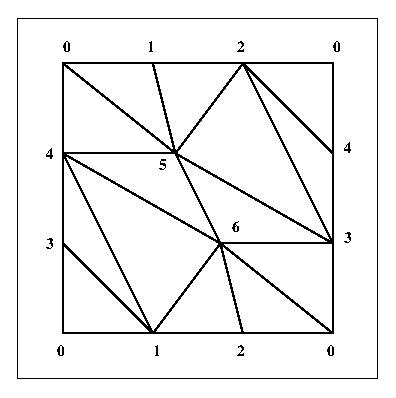
\includegraphics{torus2.eps}}
\vskip 0.40cm
%
The vertices will be named {\tt v0}, {\tt v1}, ..., {\tt v6}, {\tt v0} being the base point. The edges
will be named {\tt e01}, {\tt e02}, ...,  {\tt e56}, the list of faces of the edge $e_{ij}$ being
$(v_j\  v_i)$. The triangles will be named {\tt t013}, {\tt t015}, ..., {\tt t456}, the list of faces of
the triangle $t_{ijk}$ being $(e_{jk}\  e_{ik}\  e_{ij})$.
With this convention of describing the simplices, the call to {\tt build-finite-ss} is in simplified form:
{\footnotesize\begin{verbatim}
(setf torus2
    (build-finite-ss 
       '(v0  v1  v2  v3  v4  v5  v6 

         1 e01  (v1 v0)   e02  (v2 v0)   e03  (v3 v0)
           e04  (v4 v0)   e05  (v5 v0)   e06  (v6 v0)
           e12  (v2 v1)   e13  (v3 v1)   e14  (v4 v1)
           e15  (v5 v1)   e16  (v6 v1)   e23  (v3 v2)
           e24  (v4 v2)   e25  (v5 v2)   e26  (v6 v2)
           e34  (v4 v3)   e35  (v5 v3)   e36  (v6 v3)
           e45  (v5 v4)   e46  (v6 v4)   e56  (v6 v5)

         2 t013  (e13 e03 e01)  t015  (e15 e05 e01)  t024  (e24 e04 e02)
           t026  (e26 e06 e02)  t036  (e36 e06 e03)  t045  (e45 e05 e04)
           t125  (e25 e15 e12)  t126  (e26 e16 e12)  t134  (e34 e14 e13)
           t146  (e46 e16 e14)  t234  (e34 e24 e23)  t235  (e35 e25 e23)
           t356  (e56 e36 e35)  t456  (e56 e46 e45)  )))

Checking the 0-simplices...
Checking the 1-simplices...
Checking the 2-simplices...
[K1 Simplicial-Set]
\end{verbatim}}
After verification of the coherence of the description of the faces, the function
{\tt build-finite-ss} calls adequately the function {\tt build-smst} to create an instance
of the class {\tt SIMPLICIAL SET} subclass of the class {\tt CHAIN COMPLEX}. So that, it is easy for 
the user  to obtain the homology groups of the torus, for instance in dimension $1$:

{\footnotesize\begin{verbatim}
(chcm-homology  torus2 1)  ==>

Homology in dimension 1:

Component Z

Component Z
\end{verbatim}}
The function {\tt build-finite-ss} calls internally some verification functions mentioned above
to verify the coherence of the description of the simplicial set and gives 
an error message if the description of the simplicial set is incorrect. For instance:
{\footnotesize\begin{verbatim}
(setf mm (build-finite-ss 
   '(s0 s1 s2 s3 
     1 0-1 (s1 s0)  1-2 (s2 s1)  2-3 (s3 s2)
     2 0-1-2 (2-3 1-2 0-1))
  ))

Checking the 0-simplices...
Checking the 1-simplices...
Checking the 2-simplices...
Error: Noncoherent boundary operators detected by CHECK-FACES :
Simplex => <AbSm - 0-1-2>
del_0 o del_0 => <AbSm - S3>
del_0 o del_1 => <AbSm - S2>
\end{verbatim}}
\vskip 0.35cm
In the following examples, we show the power of {\tt build-finite-ss} for the description
of classical surfaces as simplicial sets, and in each case we  verify the well known 
homology groups of those surfaces. The examples of the torus
or the dunce-hat must be compared, as to the simplicity of the definition, to the respective 
ones in the previous page and in  the Homology chapter.
\newpage
%
\vskip 0.40cm
\centerline{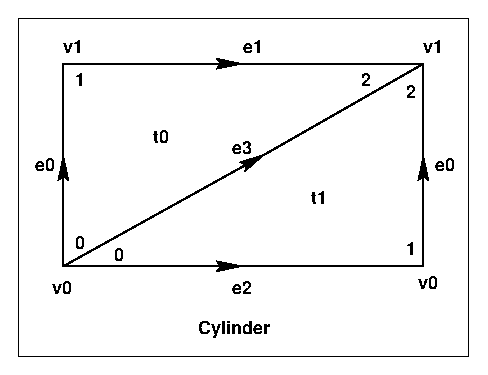
\includegraphics{cylinss.eps}}
\vskip 0.40cm
%

{\footnotesize\begin{verbatim}
(setf cylinss (build-finite-ss 
    '(v0 v1 
      1 e0 (v1 v0) e1 (v1 v1) e2 (v0 v0) e3 (v1 v0)
      2 t0 (e1 e3 e0) t1 (e0 e3 e2)) ))  ==>

[K2 Simplicial-Set]

(dotimes (i 3) (chcm-homology cylinss i)) ==>

Homology in dimension 0 :

Component Z

Homology in dimension 1 :

Component Z

Homology in dimension 2 :

---done---
\end{verbatim}}
\newpage
%
\vskip 0.40cm
\centerline{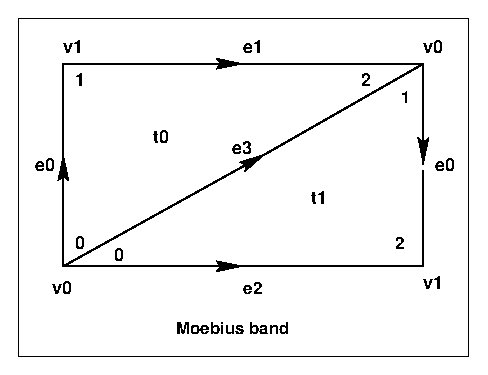
\includegraphics{moebiuss.eps}}
\vskip 0.40cm
%
{\footnotesize\begin{verbatim}
(setf moebiuss (build-finite-ss 
  '(v0 v1 
    1 e0 (v1 v0) e1 (v0 v1) e2 (v1 v0) e3 (v0 v0)
    2 t0 (e1 e3 e0) t1 (e0 e2 e3)) ))  ==>

[K3 Simplicial-Set]

(dotimes (i 3) (chcm-homology moebiuss i)) ==>

Homology in dimension 0 :

Component Z

Homology in dimension 1 :

Component Z

Homology in dimension 2 :

---done---
\end{verbatim}}
\newpage
%
\vskip 0.40cm
\centerline{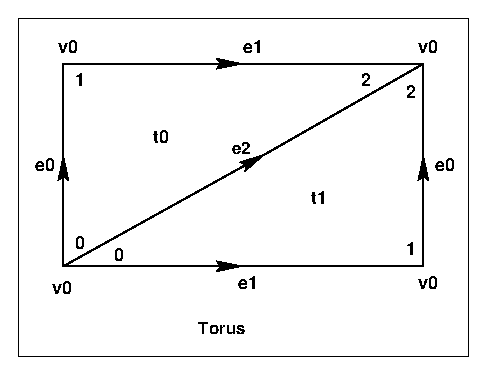
\includegraphics{toruss.eps}}
\vskip 0.40cm
%
{\footnotesize\begin{verbatim}
(setf toruss (build-finite-ss 
  '(v0
    1 e0 (v0 v0) e1 (v0 v0) e2 (v0 v0)
    2 t0 (e1 e2 e0) t1 (e0 e2 e1)) ))           ==>

[K4 Simplicial-Set]

(dotimes (i 3) (chcm-homology toruss i))  ==>

Homology in dimension 0 :

Component Z

Homology in dimension 1 :

Component Z

Component Z

Homology in dimension 2 :

Component Z

---done---
\end{verbatim}}
\newpage
%
\vskip 0.40cm
\centerline{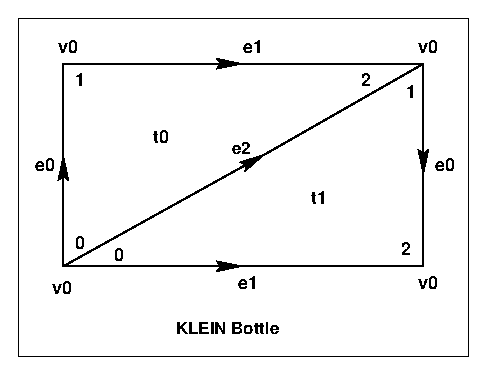
\includegraphics{bottless.eps}}
\vskip 0.40cm
%
{\footnotesize\begin{verbatim}
(setf bottless (build-finite-ss 
  '(v0
    1 e0 (v0 v0) e1 (v0 v0) e2 (v0 v0)
    2 t0 (e1 e2 e0) t1 (e0 e1 e2)) ))           ==>

[K5 Simplicial-Set]

(dotimes (i 3) (chcm-homology bottless i))  ==>

Homology in dimension 0 :

Component Z

Homology in dimension 1 :

Component Z/2Z

Component Z

Homology in dimension 2 :

---done---
\end{verbatim}}
\newpage
%
\vskip 0.40cm
\centerline{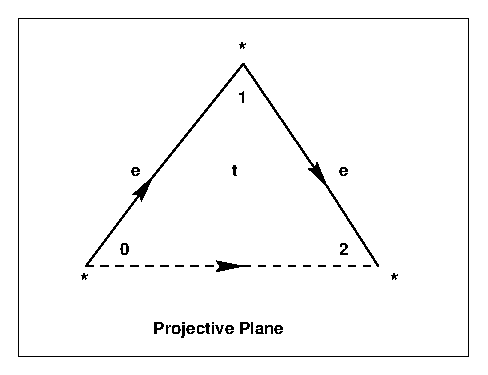
\includegraphics{ppss.eps}}
\vskip 0.40cm
%
{\footnotesize\begin{verbatim}
(setf ppss (build-finite-ss 
  '( *
     1 e (* *)
     2 t (e * e)) ))             ==>

[K6 Simplicial-Set]

(dotimes (i 3) (chcm-homology ppss i))  ==>

Homology in dimension 0 :

Component Z

Homology in dimension 1 :

Component Z/2Z

Homology in dimension 2 :

---done---
\end{verbatim}}
The user will note that the list of faces for the $2$--simplex {\tt t}, is
in simplified form. In particular, as the face $1$ of {\tt t} is the $0$--degeneracy
of the base point ``$*$'', it is sufficient to code the  face $1$ of {\tt t}
by ``{\tt *}'' instead of the complete form {\tt (0 *)}.
\newpage
%
\vskip 0.40cm
\centerline{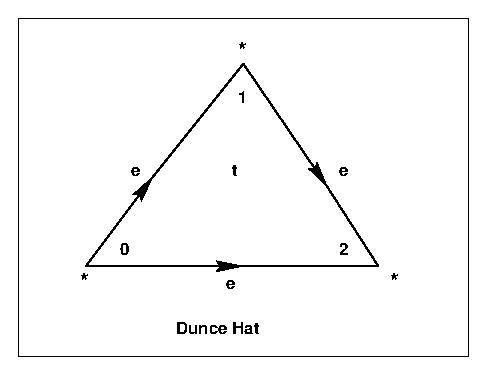
\includegraphics{duncess.eps}}
\vskip 0.40cm
%
{\footnotesize\begin{verbatim}
(setf duncess (build-finite-ss 
  '( *
     1 e (* *)
     2 t (e e e)) ))  ==>
 
[K7 Simplicial-Set]

(dotimes (i 3) (chcm-homology duncess i))  ==>

Homology in dimension 0 :

Component Z

Homology in dimension 1 :

Homology in dimension 2 :

---done---
\end{verbatim}}
\newpage

\section {Special simplicial sets}

The system provides useful functions to create interesting simplicial sets of constant usage.
In particular, the user is advised from now to use the following version of the standard
simplex implemented in {\tt Kenzo} and not the one given previously for simplicity reason. 

\subsection {The standard simplex}
{\parindent=0mm
{\leftskip=5mm 
{\tt delta} {\em dmns} \hfill {\em [Function]} \par}
{\leftskip=15mm 
Create\index{standard simplex} the standard simplex $\Delta^n$ with vertices $0,1,\ldots,n$,  
where {\em dmns} is the parameter for $n$.
This simplicial set is so important in the applications that
the implementor has decided to code the simplices in a  way similar to the coding\index{standard simplex!coding} 
of the degeneracy operators.
An {\bf increasing} sequence of non-negative integers describing a simplex, is coded
on a binary integer with the following convention: a number $i$ representing the vertex $i$ 
is the $(i+1)$--th binary bit of a machine word. The base point $0$ is the bit 1 in position 1 of the
word. This representation is very efficient for saving memory space but somehow awkward to read. \par}
{\leftskip=5mm 
{\tt delta-infinity} \hfill {\em [Function]} \par}
{\leftskip=15mm 
Create the locally effective standard simplex $\Delta^{\N}$ freely generated by the positive integers. \par}
{\leftskip=5mm 
{\tt deltab} \hfill {\em [Function]} \par}
{\leftskip=15mm 
Create the locally effective {\bf reduced} simplicial set $\bar \Delta$, built from
$\Delta^{\N}$ by identifying all the vertices to the base point. \par}
{\leftskip=5mm 
{\tt deltab2} \hfill {\em [Function]} \par}
{\leftskip=15mm 
Create the locally effective {\bf 1--reduced} simplicial set $\Delta_2^{\N}$, obtained from the above $\bar \Delta$,
by identification of all the edges with the base point. This is the efficient version of the coalgebra 
that is used as example in the cobar chapter. \par}
{\leftskip=5mm 
{\tt dlop-ext-int} {\em ext-dlop} \hfill {\em [Function]}\par}
{\leftskip=15mm 
Code on an integer the valid list (increasing order) representing the simplex {\em ext-dlop} of the
standard simplex. \par}
{\leftskip=5mm 
{\tt dlop-int-ext} {\em dgop} \hfill {\em [Function]}\par}
{\leftskip=15mm 
Give the list representing a simplex of the standard simplex from the integer {\em dgop}. \par}
}
\newpage
{\parindent=0mm
{\leftskip=5mm 
{\tt vertex-i} {\em absm i} \hfill {\em [Function]}\par}
{\leftskip=15mm 
Give the $i$--th vertex of the (coded, degenerate or not) abstract simplex {\em absm} belonging to a simplicial set
of the $\Delta$ family. \par}
{\leftskip=5mm 
{\tt absm-ext-int} {\em vlist} \hfill {\em [Function]}\par}
{\leftskip=15mm 
Create a valid abstract simplex of the $\Delta$ family from the simplex {\em vlist} written as a non-decreasing list of 
non--negative integers (i.e coding of any degenerate or non--degenerate simplex of the $\Delta$ fa\-mi\-ly). \par}
{\leftskip=5mm 
{\tt absm-int-ext} {\em absm} \hfill {\em [Function]}\par}
{\leftskip=15mm 
From an internal coded form of an abstract simplex of the $\Delta$ family, create the  non-decreasing list
of non--negative integers representing the canonical external form of such a simplex. \par}
{\leftskip=5mm 
{\tt soft-delta} {\em dmns} \hfill {\em [Function]} \par}
{\leftskip=15mm 
Create another version of the standard simplex $\Delta^n$ designed for a better clarity in
the printing of the results at testing time. More precisely, the simplices are represented internally by a list
of the form {\tt (:delt {\em binary-code})}. With this representation, the system is able to
recognize a coded simplex and to print it in a readable form. For the user, the only
requirement is to write a simplex coded $n$ as {\tt (d {\em n})}, where {\tt d} is the macro
building the internal representation (see the examples). Attention: the above conversion
functions do not work with this representation. \par}
{\leftskip=5mm 
{\tt soft-delta-infinity} \hfill {\em [Function]} \par}
{\leftskip=15mm 
Create another version of the locally effective standard simplex $\Delta^{\N}$ 
(see the function {\tt soft-delta} above). \par}
}

\subsection* {Examples}

{\footnotesize\begin{verbatim}
(setf d3 (delta 3))  ==>

[K8 Simplicial-Set]
\end{verbatim}}
The simplices $2$, $4$ and  $8$ are the coded representation of the vertices $1$, $2$ and $3$:
{\footnotesize\begin{verbatim}
(cmpr d3 2 4)  ==>

:LESS

(cmpr d3 4 4)  ==>

:EQUAL

(cmpr d3 8 4)  ==>

:GREATER
\end{verbatim}}
The list returned by the following statement  getting the basis of $\Delta^3$ in 
dimension $2$, namely {\tt (7 11 13 14)} is in fact the coded list 
of the following simplices {\tt ((0 1 2) (0 1 3) (0 2 3) (1 2 3))}. 
{\footnotesize\begin{verbatim}
(basis d3 2)  ==>

(7 11 13 14)
\end{verbatim}}
In the following statement, 
the integer $21$ represents the simplex in dimension $2$, {\tt (0 1 4)}, $1$ represents the operator $\partial_1$
and the face is therefore {\tt (0 4)} represented as the integer $17$. 
{\footnotesize\begin{verbatim}
(face d3 1 2 21)  ==>

<AbSm - 17>
\end{verbatim}}
We may obtain the same result, using:
{\footnotesize\begin{verbatim}
(face d3 1 2 (dlop-ext-int '(0 1 4)))  ==>

<AbSm - 17>
\end{verbatim}}
Let us test the conversion functions.
{\footnotesize\begin{verbatim}
(vertex-i (absm 0 1) 0)  ==>

0

(vertex-i (absm 1 1) 0)  ==>

0

(vertex-i (absm 1 1) 1)  ==>

0

(vertex-i (absm 0 7) 2)  ==>

2

(absm-ext-int '(0 0 0 1 2 3 3 3))  ==>

<AbSm 6-5-1-0 15>

(absm-ext-int '(0 1 1 1 2))  ==>

<AbSm 2-1 7>

(absm-int-ext (absm-ext-int '(0 0 0 1 2 3 3 3)))  ==>

(0 0 0 1 2 3 3 3)
\end{verbatim}}
The following  call to the macro {\tt ?} returns the boundary of the simplex {\tt (0 2 3)}
of $\Delta^3$, the integers $5$, $9$ and $12$ representing respectively the simplices
{\tt (0 2)}, {\tt (0 3)} and {\tt (2 3)}. The application of the coproduct {\tt dgnl} to the
simplex {\tt (0 1 2 3)}, coded $15$, is also easily interpreted:
{\footnotesize\begin{verbatim}
(? d3 2 13)

-----------------------------------------------------------------------{CMB 1}
<1 * 5>
<-1 * 9>
<1 * 12>
------------------------------------------------------------------------------

(dgnl d3 3 15)  ==>

----------------------------------------------------------------------{CMBN 3}
<1 * <TnPr 1 15>>
<1 * <TnPr 3 14>>
<1 * <TnPr 7 12>>
<1 * <TnPr 15 8>>
------------------------------------------------------------------------------
\end{verbatim}}
We may show now some examples with the {\it soft} version of the standard
simplex. Using the macro {\tt d} and the function {\tt dlop-ext-int} the user may work
with a readable form of the simplices and the degeneracy operators.
{\footnotesize\begin{verbatim}
(setf d3 (soft-delta 3))  ==>

[K10 Simplicial-Set]

(cmpr d3 (d 2) (d 4))  ==>

:LESS

(basis d3 1)  ==>

(0-1 0-2 1-2 0-3 1-3 2-3)
\end{verbatim}}
\newpage
{\footnotesize\begin{verbatim}
(dgnl d3 3 (d (dlop-ext-int '(0 1 2 3))))  ==>

----------------------------------------------------------------------{CMBN 3}
<1 * <TnPr 0 0-1-2-3>>
<1 * <TnPr 0-1 1-2-3>>
<1 * <TnPr 0-1-2 2-3>>
<1 * <TnPr 0-1-2-3 3>>
------------------------------------------------------------------------------

(face d3 1 2 (d (dlop-ext-int '(0 2 4))))  ==>

<AbSm - 0-4>

(? d3 2 (d (dlop-ext-int '(0 2 3))))  ==>

----------------------------------------------------------------------{CMBN 1}
<1 * 0-2>
<-1 * 0-3>
<1 * 2-3>
------------------------------------------------------------------------------
\end{verbatim}}
\newpage

\subsection {Spheres, Moore spaces and projectives spaces}
{\parindent=0mm
{\leftskip=5mm 
{\tt sphere} {\em n} \hfill {\em [Function]} \par}
{\leftskip=15mm 
Create\index{sphere} a simplicial set, a model  for the sphere of dimension $n$, ($n \geq 0$). 
This is a typical example where the differential is known a priori to be null, so the {\tt :intr-bndr}
keyword parameter is set to function {\tt zero-pure-dffr}.
This function generates a name {\tt S{\em n}} for the {\bf unique} simplex of dimension $n$
whose faces are the degeneracies of the base point labelled ``{\tt *}''.  \par}  
{\leftskip=5mm 
{\tt sphere-wedge} {\em dmns1 ... dmnsn} \hfill {\em [Function]} \par}
{\leftskip=15mm 
Create\index{sphere!wedge} a simplicial set for the wedge of spheres. Here, the $dmns_i$ are integers,
namely the dimensions of the spheres to be wedged. The differential is null.
In the  representation created by the software, the $0$--simplex (base point) is labelled
``{\tt *}'' and in dimension $p$ the simplexes are labelled {\tt S{\em p}-{\em 1}}, ..., 
{\tt S{\em p}-{\em s}},  where
{\em s} is the number of spheres of dimension $p$ in the wedge. (See the example). \par}
{\leftskip=5mm 
{\tt moore} {\em  p n} \hfill {\em [Function]}\par}
{\leftskip=15mm 
Construct\index{Moore space} a simplicial set, a model for  ${\rm Moore}({\Z}/{p{\Z}},n)$. 
The integers $p$ and $n$ must satisfy  the conditions $p>1,\ n> 2p-4$, otherwise
the result is undefined. 
${\rm Moore}({\Z}/{p{\Z}},n)$ is a space, whose the only non--null homology groups are $H_0={\Z}$
and $H_n={\Z}/{p{\Z}}$. A Moore space has only three non--degenerate simplices, namely in dimension
$0$, $n$ and $n+1$. A number $p$ of faces of the  $(n+1)$--simplex are identified with the $n$--simplex, 
the others faces being contracted on the base point.
In the  representation created by the software, the $0$--simplex (base point),
the $n$--simplex and the $(n+1)$--simplex are respectively labelled
``{\tt *}'', {\tt M{$n$}} and {\tt N{$n'$}}, where $n'=n+1$. \par}
{\leftskip=5mm 
{\tt R-proj-space \&optional} {\em k l} \hfill {\em [Function]} \par}
{\leftskip=15mm 
If $k=1$ or omitted, build a simplicial set model\index{projective spaces} of $K({\Z}_2,1)= P^\infty {\R}$. 
In dimension $n$, this simplicial set has only one non-degenerate simplex, namely the integer $n$. 
The faces of this non-degenerate simplex $n$ are given by the following formulas:
$\partial_0 n = \partial_n n = n-1$ and for $i \not= 0$ and $i \not=n$,  $\partial_i n= \eta_{i-1} (n-2)$.  
If $k >1$, build an 
analogous simplicial set but with no simplices in dimensions $1 \leq m < k$. If in addition to $k$ 
the argument $l$, ($l \geq k$), is provided, build
an analogous simplicial set but with no simplices in dimensions $m \geq l$. \par 
}

\subsection*{Examples}

Let us define first, an auxiliary function {\tt show-structure}\index{function {\tt show-structure}} 
with $2$ arguments {\em ss} and {\em dmn},
to show the structure (i.e. generators and faces) of the simplicial set  {\em ss},  
from the dimension $0$ up to the dimension {\em dmn} included.
{\footnotesize\begin{verbatim}
(defun show-structure (ss dmn)
 (dotimes (i (1+ dmn))
   (format t "~2%Dimension = ~D :" i)
   (case i
     (0 (format t "~2%~8TVertices : ~8T~A" (basis ss 0)))
     (otherwise
        (dolist (s (basis ss i))
            (format t "~2%~8TSimplex : ~A~2%~16TFaces : ~A"
                    s (mapcar #'(lambda (j) (face ss j i s))
                                (<a-b> 0 i)))))
  )))
\end{verbatim}}
In these elementary examples, we show the structure of some simplicial sets built
from the functions above. Let us begin with $S^2$.

{\footnotesize\begin{verbatim}
(setf s2 (sphere 2))  ==>

[K11 Simplicial-Set]

(bspn s2)  ==>

*
\end{verbatim}}
Applying the function {\tt basis}, we see that the only non-null simplices are in dimension $0$
and $2$.
{\footnotesize\begin{verbatim}
(dotimes (i 4) (print (basis s2 i)))  ==>

(*) 
NIL 
(S2) 
NIL 
\end{verbatim}}
In dimension $2$, the $3$ faces of the simplicial set are all the degeneracy $\eta_0$ 
of the base point.
{\footnotesize\begin{verbatim}
(mapcar #'(lambda(i)(face s2 i 2 's2)) '(0 1 2))  ==>

(<AbSm 0 *> <AbSm 0 *> <AbSm 0 *>)

(face s2 5 7 (absm (dgop-ext-int '(5 3 1 0)) 's2))  ==>

<AbSm 3-1-0 S2>

(face s2 2 7 (absm (dgop-ext-int '(5 3 1 0)) 's2))  ==>

<AbSm 4-2-0 S2>
\end{verbatim}}
The differential of the simplex {\tt s2} in dimension $2$ is of course the null combination
of degree $1$:
{\footnotesize\begin{verbatim}
(? s2 2 's2)  ==>

-----------------------------------------------------------------------{CMB 1}
------------------------------------------------------------------------------

\end{verbatim}}

Now, let us see the stucture of $S^3$, using our auxiliary function {\tt show-structure}.
{\footnotesize\begin{verbatim}
(setf s3 (sphere 3))  ==>

[K12 Simplicial-Set]

(show-structure s3 3)  ==>

Dimension = 0 :

        Vertices :  (*)

Dimension = 1 :

Dimension = 2 :

Dimension = 3 :

        Simplex : S3

                Faces : (<AbSm 1-0 *> <AbSm 1-0 *> <AbSm 1-0 *> <AbSm 1-0 *>)
\end{verbatim}}

The space ${\rm Moore}(2,1)$ is the projective plane:
{\footnotesize\begin{verbatim}

(setf p2 (moore 2 1))  ==>

[K13 Simplicial-Set]

(show-structure p2 2)  ==>

Dimension = 0 :

        Vertices :  (*)

Dimension = 1 :

        Simplex : M1

                Faces : (<AbSm - *> <AbSm - *>)

Dimension = 2 :

        Simplex : N2

                Faces : (<AbSm - M1> <AbSm 0 *> <AbSm - M1>)
\end{verbatim}}
In the following example, note the identification of $p$ faces 
of the $(n+1)$--simplex with the $n$--simplex.
{\footnotesize\begin{verbatim}
(setf sp2r (moore 2 2))  ==>

[K15 Simplicial-Set]

(show-structure sp2r 3)  ==>

Dimension = 0 :

        Vertices :  (*)

Dimension = 1 :

Dimension = 2 :

        Simplex : M2

                Faces : (<AbSm 0 *> <AbSm 0 *> <AbSm 0 *>)

Dimension = 3 :

        Simplex : N3

                Faces : (<AbSm - M2> <AbSm 1-0 *> <AbSm - M2>
                         <AbSm 1-0 *>)

\end{verbatim}}
Let us see an example of a wedge of spheres:
{\footnotesize\begin{verbatim}
(setf w (sphere-wedge 3 2 3))  ==>

[K16 Simplicial-Set]

(show-structure w 5)  ==>

Dimension = 0 :

        Vertices :  (*)

Dimension = 1 :

Dimension = 2 :

        Simplex : S2-1

                Faces : (<AbSm 0 *> <AbSm 0 *> <AbSm 0 *>)

Dimension = 3 :

        Simplex : S3-1

                Faces : (<AbSm 1-0 *> <AbSm 1-0 *> <AbSm 1-0 *>
                         <AbSm 1-0 *>)

        Simplex : S3-2

                Faces : (<AbSm 1-0 *> <AbSm 1-0 *> <AbSm 1-0 *>
                         <AbSm 1-0 *>)

Dimension = 4 :

Dimension = 5 :

(cmpr w 's3-1 's3-2)  ==>

:LESS

(face w 2 3 's3-1)  ==>

<AbSm 1-0 *>

(? w 3 's3-2)  ==>

-----------------------------------------------------------------------{CMB 2}
------------------------------------------------------------------------------
\end{verbatim}}
\newpage
Let us show now some examples with the simplicial sets generated by the
function {\tt R-proj-space}.
{\footnotesize\begin{verbatim}
(setf p1 (R-proj-space))  ==>

[K20 Simplicial-Set]

(dotimes (i 7)(print(basis p1 i)))  ==>

(0) 
(1) 
(2) 
(3) 
(4) 
(5) 
(6) 

(show-structure p1 5)  ==>

Dimension = 0 :

        Vertices :  (0)

Dimension = 1 :

        Simplex : 1

                Faces : (<AbSm - 0> <AbSm - 0>)

Dimension = 2 :

        Simplex : 2

                Faces : (<AbSm - 1> <AbSm 0 0> <AbSm - 1>)

Dimension = 3 :

        Simplex : 3

                Faces : (<AbSm - 2> <AbSm 0 1> <AbSm 1 1> <AbSm - 2>)

Dimension = 4 :

        Simplex : 4

                Faces : (<AbSm - 3> <AbSm 0 2> <AbSm 1 2> <AbSm 2 2> <AbSm - 3>)

Dimension = 5 :

        Simplex : 5

                Faces : (<AbSm - 4> <AbSm 0 3> <AbSm 1 3> <AbSm 2 3> <AbSm 3 3> 
                         <AbSm - 4>)

(dotimes (i 5)(chcm-homology p1 i)) ==>

Homology in dimension 0 :

Component Z

Homology in dimension 1 :

Component Z/2Z

Homology in dimension 2 :

---done---

Homology in dimension 3 :

Component Z/2Z

Homology in dimension 4 :

---done---

(setf p2 (R-proj-space 2))  ==>

[K21 Simplicial-Set]

(show-structure p2 5)  ==>

Dimension = 0 :

        Vertices :  (0)

Dimension = 1 :

Dimension = 2 :

        Simplex : 2

                Faces : (<AbSm 0 0> <AbSm 0 0> <AbSm 0 0>)

Dimension = 3 :

        Simplex : 3

                Faces : (<AbSm - 2> <AbSm 1-0 0> <AbSm 1-0 0> <AbSm - 2>)

Dimension = 4 :

        Simplex : 4

                Faces : (<AbSm - 3> <AbSm 0 2> <AbSm 1 2> <AbSm 2 2> <AbSm - 3>)

Dimension = 5 :

        Simplex : 5

                Faces : (<AbSm - 4> <AbSm 0 3> <AbSm 1 3> <AbSm 2 3> <AbSm 3 3> 
                         <AbSm - 4>)

(dotimes (i 5)(chcm-homology p2 i))  ==>

Homology in dimension 0 :

Component Z

Homology in dimension 1 :

---done---

Homology in dimension 2 :

Component Z

Homology in dimension 3 :

Component Z/2Z

Homology in dimension 4 :

---done---

(setf pr3 (R-proj-space 3))  ==>

[K22 Simplicial-Set]

(show-structure pr3 4)  ==>

Dimension = 0 :

        Vertices :  (0)

Dimension = 1 :

Dimension = 2 :

Dimension = 3 :

        Simplex : 3

                Faces : (<AbSm 1-0 0> <AbSm 1-0 0> <AbSm 1-0 0> <AbSm 1-0 0>)

Dimension = 4 :

        Simplex : 4

                Faces : (<AbSm - 3> <AbSm 2-1-0 0> <AbSm 2-1-0 0> 
                         <AbSm 2-1-0 0> <AbSm - 3>)

(dotimes (i 7)  (print (? pr3 i i)))  ==>

----------------------------------------------------------------------{CMBN -1}
------------------------------------------------------------------------------

----------------------------------------------------------------------{CMBN 0}
------------------------------------------------------------------------------

----------------------------------------------------------------------{CMBN 1}
------------------------------------------------------------------------------

----------------------------------------------------------------------{CMBN 2}
------------------------------------------------------------------------------

----------------------------------------------------------------------{CMBN 3}
<2 * 3>
------------------------------------------------------------------------------

----------------------------------------------------------------------{CMBN 4}
------------------------------------------------------------------------------

----------------------------------------------------------------------{CMBN 5}
<2 * 5>
------------------------------------------------------------------------------
\end{verbatim}}
Let us use now the parameter {\em l}, allowing the truncation in the upper dimensions.
{\footnotesize\begin{verbatim}
(setf p12 (R-proj-space 1 2))  ==>

[K23 Simplicial-Set]

(show-structure p12 2)  ==>

Dimension = 0 :

        Vertices :  (0)

Dimension = 1 :

        Simplex : 1

                Faces : (<AbSm - 0> <AbSm - 0>)

Dimension = 2 :
\end{verbatim}}
Setting $k=l$ does not creates something amazing!
{\footnotesize\begin{verbatim}
(setf p22 (R-proj-space 2 2))  ==>

[K28 Simplicial-Set]

(show-structure p22 2)  ==>

Dimension = 0 :

        Vertices :  (0)

Dimension = 1 :

Dimension = 2 :

(setf p47 (R-proj-space 4 7))  ==>

[K33 Simplicial-Set]

(show-structure p47 8)  ==>

Dimension = 0 :

        Vertices :  (0)

Dimension = 1 :

Dimension = 2 :

Dimension = 3 :

Dimension = 4 :

        Simplex : 4

                Faces : (<AbSm 2-1-0 0> <AbSm 2-1-0 0> <AbSm 2-1-0 0> 
                         <AbSm 2-1-0 0> <AbSm 2-1-0 0>)

Dimension = 5 :

        Simplex : 5

                Faces : (<AbSm - 4> <AbSm 3-2-1-0 0> <AbSm 3-2-1-0 0> 
                         <AbSm 3-2-1-0 0> <AbSm 3-2-1-0 0> <AbSm - 4>)

Dimension = 6 :

        Simplex : 6

                Faces : (<AbSm - 5> <AbSm 0 4> <AbSm 1 4> <AbSm 2 4> 
                         <AbSm 3 4> <AbSm 4 4> <AbSm - 5>)

Dimension = 7 :

Dimension = 8 :
\end{verbatim}}

\newpage

\section {Cartesian product of  simplicials sets }

Let $X$ and $Y$ be two simplicial\index{simplicial sets!cartesian product}
sets, the construction of $X\times Y$ is based on the very definition $(X\times Y)_n =X_n\times Y_n$
where $X_n$, $Y_n$ and $(X\times Y)_n$ are the {\em possibly degenerate} simplices of $X$, $Y$ and $X\times Y$
respectively. A simplex of the product $X\times Y$ is characterized  by its projections on the factors $X$ and $Y$.
\par
The {\em non--degenerate} simplices of $X\times Y$  are
represented internally in the system by a lisp object of the form:
\begin{center}
{\tt (:crpr ({\em dgop1}.{\em gmsm1}).({\em dgop2}.{\em gmsm2}))}
\end{center}
where,
\begin{enumerate}
\item {\tt dgop1} is an integer representing a coded degeneracy operator.
\item {\tt gmsm1} is a non-degenerate simplex of $X$, to which is applied the degeneracy operator
{\tt dgop1}.
\item {\tt dgop2} is an integer representing a coded degeneracy operator.
\item {\tt gmsm2} is a non-degenerate simplex of $Y$, to which is applied the degeneracy operator
{\tt dgop2}.
\end{enumerate}
This object must be a {\em non--degenerate} simplex of $X \times Y$,
that is to say, the degeneracy operators {\tt dgop1} and {\tt dgop2} must not have a common $\eta_j$, and 
therefore their list representations must have a void intersection.
The coded representation by  binary bit positions, has the same property. The corresponding type
is {\tt CRPR}.
To construct such an object, one may use the macro {\tt crpr}. As usual, a printing method
has been defined to reflect the structure of the product under the form:
\begin{center}
{\tt <CrPr {\em ext-dgop1 gmsm1 ext-dgop2 gmsm2}> }
\end{center}
where  the sequence of the operators $\eta_i$ is printed in explicit form (this is the meaning of {\em ext-dgop}).
If this sequence of $\eta_i$  is void, i.e. if the simplex {\em gmsm} is not degenerate, 
the symbol {\tt -} is printed instead.
\newpage

\subsection {Functions and macros for the product of simplicial sets}

{\parindent=0mm
{\leftskip=5mm 
{\tt crpr} {\em dgop1 gmsm1 dgop2 gmsm2} \hfill {\em [Macro]} \par}
{\leftskip=15mm 
Build an object of type {\tt CRPR}, using directly the integer coding for the
degeneracy operators. The arguments {\em gmsm1} and {\em gmsm2} are non-degenerate
simplices.  \par}
{\leftskip=5mm 
{\tt crpr} {\em absm1 absm2} \hfill {\em [Macro]} \par}
{\leftskip=15mm 
Build an object of type {\tt CRPR}, using two abstract simplices {\em absm1} and {\em absm2}. If these
abstract simplices are degenerate, the de\-ge\-ne\-ra\-cy operators must verify the condition of
the definition, i.e. no common $\eta_i$. \par}
{\leftskip=5mm 
{\tt 2absm-acrpr} {\em absm1 absm2} \hfill {\em [Function]} \par}
{\leftskip=15mm 
Build an abstract simplex, i.e. object of type {\tt ABSM}, cartesian pro\-duct of both abstract simplices {\em absm1} 
and {\em absm2}. In contrast with the previous function, there is no condition upon the
de\-ge\-ne\-ra\-cy operators of the abstract simplices. Of course, the function {\tt 2absm-acrpr} returns
a legal abstract simplex. \par}
{\leftskip=5mm 
{\tt crpr-p} {\em object} \hfill {\em [Predicate]} \par}
{\leftskip=15mm 
Test if {\em object} is of type {\tt CRPR}. \par}
{\leftskip=5mm 
{\tt dgop1} {\em crpr} \hfill {\em [Macro]} \par}
{\leftskip=15mm 
Select the degeneracy operator {\em dgop1} from the object {\tt crpr}. \par}
{\leftskip=5mm 
{\tt gmsm1} {\em crpr} \hfill {\em [Macro]} \par}
{\leftskip=15mm 
Select the geometric simplex {\em gmsm1} from the object {\tt crpr}. \par}
{\leftskip=5mm 
{\tt dgop2} {\em crpr} \hfill {\em [Macro]} \par}
{\leftskip=15mm 
Select the degeneracy operator {\em dgop2} from the object {\tt crpr}. \par}
{\leftskip=5mm 
{\tt gmsm2} {\em crpr} \hfill {\em [Macro]} \par}
{\leftskip=15mm 
Select the geometric simplex {\em gmsm2} from the object {\tt crpr}. \par}
{\leftskip=5mm 
{\tt absm1} {\em crpr} \hfill {\em [Macro]} \par}
{\leftskip=15mm 
Build the abstract simplex {\tt (absm {\em dgop1 gmsm1})} from {\em crpr}. \par}
{\leftskip=5mm 
{\tt absm2} {\em crpr} \hfill {\em [Macro]} \par}
{\leftskip=15mm 
Build the abstract simplex {\tt (absm {\em dgop2 gmsm2})} from {\em crpr}. \par}
{\leftskip=5mm 
{\tt crts-prdc} {\em smst1 smst2} \hfill {\em [Function]} \par}
{\leftskip=15mm 
Build the simplicial set, cartesian product $smst1 \times smts2$. \par}
}

\subsection* {Examples}

In the first example, note that the coded representations of $\eta_1$ and $\eta_2$ are
respectively $2$ and $4$, but these degeneracy operators appear clearly as $1$ and $2$ in the printed result.
In the second statement, the integer $28$ is the coded representation of the degeneracy {\tt (4 3 2)}.
{\footnotesize\begin{verbatim}
(crpr 2 'a 4 'b)  ==>

<CrPr 1 A 2 B>

(crpr 0 '(0 1 2 3 4 5) 28 '(0 1 2))   ==>

<CrPr - (0 1 2 3 4 5) 4-3-2 (0 1 2)>
\end{verbatim}}
For more clarity, one may also write:
{\footnotesize\begin{verbatim}
(crpr 0 '(0 1 2 3 4 5) (dgop-ext-int '(4 3 2)) '(0 1 2))   ==>

<CrPr - (0 1 2 3 4 5) 4-3-2 (0 1 2)>
\end{verbatim}}
In the following example, we see that both functions {\tt crpr} and
{\tt 2absm-acrpr} return the same geometric simplex,
{\footnotesize\begin{verbatim}
(crpr (absm 4 'a)(absm 3 'b))  ==>

<CrPr 2 A 1-0 B>

(2absm-acrpr (absm 4 'a)(absm 3 'b))  ==>

<AbSm - <CrPr 2 A 1-0 B>>
\end{verbatim}}
whereas, in the following call to {\tt crpr}, the condition upon the degeneracy
operator is not respected and the result is an illegal cartesian product.
The function {\tt 2absm-acrpr} returns the correct answer.
{\footnotesize\begin{verbatim}
(crpr (absm 5 'a)(absm 3 'b))  ==>

<CrPr 2-0 A 1-0 B>     ;;; ILLEGAL!

(2absm-acrpr (absm 5 'a) (absm 3 'b))  ==>

<AbSm 0 <CrPr 1 A 0 B>>
\end{verbatim}}
The following example is particularly instructive. The simplicial set
whose the realization is homeomorphic to the  square is built by using the product of two segments.
A call like {\tt (delta n)} builds  the standard $n$--simplex. So first, we generate
two copies {\tt X} and {\tt Y} of the standard $1$--simplex and we list the abstract simplices 
up to dimension $2$ for a better understanding of the components of the product {\tt XY}.
{\footnotesize\begin{verbatim}
(setf X (delta 1))  ==>

[K4 Simplicial-Set]

(setf Y X)  ==>

[K4 Simplicial-Set]
\end{verbatim}}
%
\vskip 0.40cm
\centerline{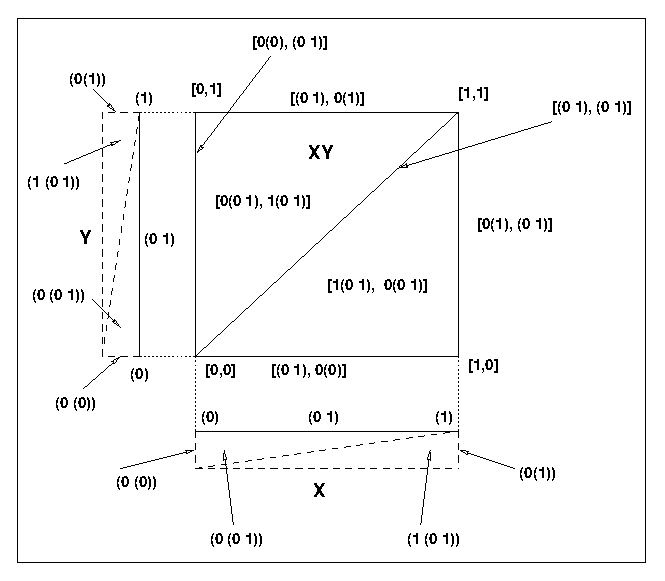
\includegraphics{ssquare.eps}}
\vskip 0.40cm
%

In list representation (non-coded simplices), the  abstract simplices of $X$ up to the dimension $2$, 
including the degenerate ones are:
\begin{itemize}
\item {Dimension 0}: {\footnotesize {\tt <AbSm - (0)>, <AbSm - (1)>}}. 
\item {Dimension 1}: {\footnotesize {\tt <AbSm 0 (0)>,  <AbSm 0 (1)>,  <AbSm - (0 1)>}}. 
\item {Dimension 2}: {\footnotesize {\tt <AbSm 1-0 (0)>, <AbSm 1-0 (1)>,  <AbSm 0 (0 1)>, \par
 <AbSm 1 (0 1)>}}.
\end{itemize}

Let us look first at the non-degenerate simplices of the simplicial set $X \times Y$. Those simplices are objects
of type  {\tt CRPR}. In dimension $1$, we see that some projections are
degeneracies of vertices and, in dimension $2$, the projections are all degeneracies of
the $1$--simplex {\tt(0 1)} coded as $3$. Nevertheless, all the listed simplices are {\em geometric} 
simplices (i.e. non-degenerate ones) of the product {\tt XY}. The diagram above shows the relationship between
the $3$ simplicial sets. 
{\footnotesize\begin{verbatim}
(setf XY (crts-prdc X Y))  ==>

[K5 Simplicial-Set]

(show-structure XY 2)  ==>

Dimension = 0 :

        Vertices :  (<CrPr - 1 - 1> <CrPr - 1 - 2> <CrPr - 2 - 1>
                     <CrPr - 2 - 2>)

Dimension = 1 :

        Simplex : <CrPr - 3 - 3>

                Faces : (<AbSm - <CrPr - 2 - 2>>
                         <AbSm - <CrPr - 1 - 1>>)

        Simplex : <CrPr - 3 0 1>

                Faces : (<AbSm - <CrPr - 2 - 1>>
                         <AbSm - <CrPr - 1 - 1>>)

        Simplex : <CrPr - 3 0 2>

                Faces : (<AbSm - <CrPr - 2 - 2>>
                         <AbSm - <CrPr - 1 - 2>>)

        Simplex : <CrPr 0 1 - 3>

                Faces : (<AbSm - <CrPr - 1 - 2>>
                         <AbSm - <CrPr - 1 - 1>>)

        Simplex : <CrPr 0 2 - 3>

                Faces : (<AbSm - <CrPr - 2 - 2>>
                         <AbSm - <CrPr - 2 - 1>>)

Dimension = 2 :

        Simplex : <CrPr 0 3 1 3>

                Faces : (<AbSm - <CrPr - 3 0 2>>
                         <AbSm - <CrPr - 3 - 3>>
                         <AbSm - <CrPr 0 1 - 3>>)

        Simplex : <CrPr 1 3 0 3>

                Faces : (<AbSm - <CrPr 0 2 - 3>>
                         <AbSm - <CrPr - 3 - 3>>
                         <AbSm - <CrPr - 3 0 1>>)
\end{verbatim}}
To be more readable we may translate the coded representations of the de\-ge\-ne\-ra\-cy operators
and of the simplices in the list representation:
{\footnotesize\begin{verbatim}

Dimension 0 :

        Vertices : (<CrPr - (0) - (0)> 
                    <CrPr - (0) - (1)> 
                    <CrPr - (1) - (0)> 
                    <CrPr - (1) - (1)>)

Dimension 1 :

        Simplex : <CrPr 0 (0) - (0 1)>

                Faces : (<AbSm - <CrPr - (0) - (1)> >
                         <AbSm - <CrPr - (0) - (0)> >)

        Simplex : <CrPr 0 (1) - (0 1)>

                Faces : (<AbSm - <CrPr - (1) - (1)> >
                         <AbSm - <CrPr - (1) - (0)> >)

        Simplex : <CrPr - (0 1) 0 (0)>

                Faces : (<AbSm - <CrPr - (1) - (0)> >
                         <AbSm - <CrPr - (0) - (0)> >)

        Simplex : <CrPr - (0 1) 0 (1)>

                Faces : (<AbSm - <CrPr - (1) - (1)> >
                         <AbSm - <CrPr - (0) - (1)> >)

        Simplex : <CrPr - (0 1) - (0 1)>

                Faces : (<AbSm - <CrPr - (1) - (1)> >
                         <AbSm - <CrPr - (0) - (0)> >)

Dimension 2 :

        Simplex : <CrPr 0 (0 1) 1 (0 1)>

                Faces : (<AbSm - <CrPr - (0 1) 0 (1)> >
                         <AbSm - <CrPr - (0 1) - (0 1)> >
                         <AbSm - <CrPr 0 (0) - (0 1)> >)

        Simplex : <CrPr 1 (0 1) 0 (0 1)>

                Faces : (<AbSm - <CrPr 0 (1) - (0 1)> >
                         <AbSm - <CrPr - (0 1) - (0 1)> >
                         <AbSm - <CrPr - (0 1) 0 (0)> >)
\end{verbatim}}
In an analogous way, let us build the torus as the cartesian product
of two $1$--spheres. We recall that the base point of the sphere is named {\tt *}.
{\footnotesize\begin{verbatim}
(setf s1xs1 (crts-prdc (sphere 1) (sphere 1)))  ==>

[K15 Simplicial-Set]

(show-structure s1xs1 2)  ==>

Dimension = 0 :

        Vertices :  (<CrPr - * - *>)

Dimension = 1 :

        Simplex : <CrPr - S1 - S1>

                Faces : (<AbSm - <CrPr - * - *>>
                         <AbSm - <CrPr - * - *>>)

        Simplex : <CrPr - S1 0 *>

                Faces : (<AbSm - <CrPr - * - *>>
                         <AbSm - <CrPr - * - *>>)

        Simplex : <CrPr 0 * - S1>

                Faces : (<AbSm - <CrPr - * - *>>
                         <AbSm - <CrPr - * - *>>)

Dimension = 2 :

        Simplex : <CrPr 0 S1 1 S1>

                Faces : (<AbSm - <CrPr - S1 0 *>>
                         <AbSm - <CrPr - S1 - S1>>
                         <AbSm - <CrPr 0 * - S1>>)

        Simplex : <CrPr 1 S1 0 S1>

                Faces : (<AbSm - <CrPr 0 * - S1>>
                         <AbSm - <CrPr - S1 - S1>>
                         <AbSm - <CrPr - S1 0 *>>)
\end{verbatim}}
Let us verify that  $S^1\times S^1$ has  the same  homology groups as the torus.
{\footnotesize\begin{verbatim}
(dotimes (i 3)(chcm-homology s1xs1 i)) ==>
  
Homology in dimension 0 :

 Component Z

Homology in dimension 1 :

 Component Z

 Component Z

Homology in dimension 2 :

 Component Z

\end{verbatim}}
Of course, we may generate more complex products, whose basis are composed of rather long
lists of simplices as shown below. The user will also pay
attention to the fact that the composition of the macro {\tt crpr} is not associative. In the
following example, the simplicial sets located respectively by {\tt p1} and {\tt p2}
are different objects, though being canonically isomorphic.
{\footnotesize\begin{verbatim}
(setf p1 (crts-prdc (sphere 2) (crts-prdc (sphere 2) (sphere 3))))  ==>

[K20 Simplicial-Set]

(setf p2 (crts-prdc (crts-prdc (sphere 2) (sphere 2)) (sphere 3)))  ==>

[K21 Simplicial-Set]

(dotimes (i 8) (print (length (basis p1 i))))  ==>

1 
0 
3 
22 
138 
390 
480 
210 
\end{verbatim}}

\subsection* {Lisp files concerned in this chapter}

{\tt simplicial-sets.lisp}, {\tt delta.lisp}, {\tt specials-smsts.lisp}, \par
{\tt cartesian-products.lisp}. \par
[{\tt classes.lisp}, {\tt macros.lisp}, {\tt various.lisp}].

\chapter {Simplicial morphisms}

The software {\tt Kenzo} implements simplicial morphisms in a way analogous to
chain complex morphisms.\index{simplicial morphisms}

\section {Representation of a  simplicial morphism}

A simplicial morphism is  an instance\index{class!{\tt SIMPLICIAL-MRPH}} of the class {\tt SIMPLICIAL-MRPH}, 
subclass of the class {\tt MORPHISM}.
{\footnotesize\begin{verbatim}
(DEFCLASS SIMPLICIAL-MRPH (morphism)
  ((sintr :type sintr :initarg :sintr :reader sintr)))
\end{verbatim}}
It has one slot of its own:
\begin{description}
\item {{\tt sintr}}, an object of type {\tt SINTR}, in fact a lisp function defining the morphism
between the source and target simplicial sets. It must have  $2$ parameters:  a dimension (an integer)
and a geometric simplex of this dimension (a generator of any type) .
It must return  an abstract simplex, image in the target simplicial set of this geometric simplex.
\end{description}
A printing method has been associated to the class {\tt SIMPLICIAL-MRPH}.
A string like {\tt [K{\em n} Simplicial-Morphism]} is the  external representation of an instance of
such a class,  where {\em n} is the number plate of the {\tt Kenzo} object.

\section {The function build-smmr}

To\index{function!{\tt build-smmr}} facilitate the construction of instances 
of the class {\tt SIMPLICIAL-MRPH} and to free  the user to call
the standard constructor {\tt make-instance}, the software provides the function
\vskip 0.35cm
{\tt build-smmr :sorc} {\em sorc} {\tt :trgt} {\em trgt} {\tt :degr} {\em degr} {\tt :sintr} {\em sintr}
{\tt :intr} {\em intr} \par
\hspace*{22.5mm}{\tt :strt} {\em strt} {\tt :orgn} {\em orgn}
\vskip 0.35cm
defined with keyword parameters and returning an instance of the class {\tt SIMPLICIAL-MRPH}.
The keyword arguments of {\tt build-smmr} are:

\begin{itemize}
\item [--] {\em sorc}, the source object, an object of type {\tt SIMPLICIAL-SET}.
\item [--] {\em trgt}, the target object, an object of type {\tt SIMPLICIAL-SET}.
\item [--] {\em degr}, the degree of the morphism, an integer. In this chapter, we  consider only the
$0$ degree case (the usual one). The case $-1$ is particularly important: it allows to implement the notion
of twisting operator defining a fibration (See the chapter Fibration).
\item [--] {\em sintr}, the internal lisp function defining the effective mapping between simplicial sets.
If the integer {\em degr} is $0$ and if the following keyword argument {\em intr} is omitted, then 
the function {\tt build-smmr} builds a lisp function implementing the induced mapping between the
underlying source and target chain complexes. This function is installed in the slot {\tt intr}.
The strategy is then set to {\tt :gnrt}.
\item [--] {\em intr}, a user defined morphism for the underlying chain complexes. This argument is optional and
taken in account only if the degree is $0$ and in this case, supersedes the previous derived  mapping. 
The strategy is then mandatory.
If the degree is not null, the implementor has decided  to set the corresponding slot to {\tt NIL}.
\item [--] {\em strt}, the strategy, i.e. {\tt :gnrt} or {\tt :cmbn} attached to the previous function.
\item [--] {\em orgn}, a relevant comment list.
\end{itemize}

After a call to {\tt build-smmr}, the simplicial morphism instance 
is added to a list of previously constructed  ones ({\tt *smmr-list*}). 
As the other similar lists,
the list {\tt *smmr-list*} may be cleared by the function {\tt cat-init}.
\par
The effective application of a simplicial morphism upon arguments, 
is re\-a\-li\-zed with the macro {\tt ?} which  calls the adequate method
defined for this kind of objects.
\newpage
{\parindent=0mm
{\leftskip=5mm
{\tt ? \&rest} {\em args} \hfill {\em [Macro]} \par}
{\leftskip=15mm
Versatile macro for applying a simplicial morphism  indifferently
as {\tt (? {\em smmr dmns absm-or-gmsm})} or  {\tt (? {\em smmr cmbn})}. In the first case, the
third argument is either an abstract simplex or a geometric one. In the second case, if the
second argument is a combination, {\em smmr} is then considered as a chain complex  morphism and
it is the function in the slot {\tt intr} which is applied, so that it makes sense
only if the degree of the mapping is $0$. \par}
}

\subsection* {Examples}

In the following examples, we work with $\Delta_3$. We define three simplicial morphisms, {\tt sm1}, {\tt sm2}
and {\tt sm3}. In {\tt sm1}, the mapping is the identity mapping and we can see that this identity mapping
has been propagated on the underlying chain complex.
{\footnotesize\begin{verbatim}
(setf d3 (delta 3))  ==>

[K1 Simplicial-Set]

(setf sm1 (build-smmr
            :sorc d3 :trgt d3 :degr 0
            :sintr #'(lambda (dmns gmsm)
                        (absm 0 gmsm))
            :orgn '(identity delta-3)))   ==>

[K6 Simplicial-Morphism]

(? sm1 2 7)  ==>

<AbSm - 7>

(? sm1 1 (absm 1 1))  ==>

<AbSm 0 1>

(? sm1 (cmbn 2 1 7))  ==>

----------------------------------------------------------------------{CMBN 2}
<1 * 7>
------------------------------------------------------------------------------
\end{verbatim}}
In the simplicial morphism {\tt sm2}, the mapping is the ``null'' mapping. In
fact, it consists in  applying any abstract simplex in dimension $n$ upon the $n$--degenerate base point. 
Of course, in terms of chain complex, the cor\-res\-pon\-ding mapping applies any chain complex element
upon the null combination of same degree.
{\footnotesize\begin{verbatim}
(setf sm2 (build-smmr
            :sorc d3 :trgt d3 :degr 0
            :sintr #'(lambda (dmns gmsm)
                       (absm (mask dmns) 1))    ;;; mask(n)=2^n - 1 
            :orgn '(null delta-3)))  ==>

[K7 Simplicial-Morphism]

(? sm2 0 4)  ==>

<AbSm - 1>

(? sm2 2 7)  ==>

<AbSm 1-0 1>

(? sm2 1 (absm 1 1))  ==>

<AbSm 0 1>

(? sm2 3 15)  ==>

<AbSm 2-1-0 1>

(? sm2 (cmbn 3 2 15))  ==>

----------------------------------------------------------------------{CMBN 3}
------------------------------------------------------------------------------
\end{verbatim}}
In the simplicial morphism {\tt sm3}, we keep the same ``null'' mapping as in {\tt sm2}
but we choose as mapping for the underlying chain complex the opposite of any chain complex 
element.
{\footnotesize\begin{verbatim}
(setf sm3 (build-smmr
            :sorc d3 :trgt d3 :degr 0
            :sintr #'(lambda (dmns gmsm)
                       (absm (mask dmns) 1))
            :intr #'cmbn-opps
            :strt :cmbn
            :orgn '(null and opposite delta-3)))  ==>

[K8 Simplicial-Morphism]

(? sm3 3 15)  ==>

<AbSm 2-1-0 1>

(? sm3 (cmbn 3 7 15))  ==>

----------------------------------------------------------------------{CMBN 3}
<-7 * 15>
------------------------------------------------------------------------------

(? sm3 (cmbn 3 11 (dlop-ext-int '(0 1 2 3))))  ==>

----------------------------------------------------------------------{CMBN 3}
<-11 * 15>
------------------------------------------------------------------------------
\end{verbatim}}

\subsection* {Lisp files concerned in this chapter}

{\tt simplicial-mrphs.lisp}.
\par
[{\tt classes.lisp}, {\tt macros.lisp}, {\tt various.lisp}].

\chapter{The Eilenberg-Zilber module}

The functions of this module are related to the chain complex of the
pro\-duct of two simplicial sets.
They implement the Eilenberg-Mac Lane homomorphism (function {\tt eml}) 
and the Alexander-Whitney homomorphism  (function {\tt aw}).
\vskip 0.45cm
{\parindent=0mm
{\leftskip=5mm 
{\tt eml} {\em ssx ssy} \hfill {\em [Function]} \par}
{\leftskip=15mm 
build\index{homomorphism!Eilenberg-Mac Lane} the Eilenberg-Mac Lane homomorphism $\cal EML$, also called 
the {\em shuffle homomorphism}\footnote{{\bf Marvin Greenberg}, {\it Lectures on Algebraic Topology}, 
W.A. Benjamin Inc, 1967.}.
The arguments {\em ssx} and {\em ssy} represent some simplicial sets $X$ and $Y$.
The homomorphism 
$${\cal EML}:{\cal C}_*(X) \otimes {\cal C}_*(Y) \longrightarrow {\cal C}_*(X \times Y)$$
is defined by:
$${\cal EML}(\alpha \otimes \beta)= 
 \sum{{\varepsilon(\varpi)}(\eta_{j_q}\ldots \eta_{j_1}\alpha,\, \eta_{i_p}\ldots \eta_{i_1}\beta)},$$
where $X\times Y$ is the simplicial cartesian product of the two simplicial sets $X$ and $Y$,  $\alpha$ (resp. $\beta$)
is a geometric simplex of $X$ (resp. $Y$), $\eta_k$ is the $k^{th}$ degeneracy operator, the sum is
over all permutations $\varpi= (i_1 \ldots i_p j_1 \ldots j_q)$ of $(0 \ldots p+q-1)$ such that
$$ i_1 < i_2 < \cdots < i_p,\quad j_1 < j_2 < \cdots < j_q, \quad p+q=n$$
and $\varepsilon(\varpi)$ is the signature of the corresponding permutation. The sum at the right hand part determines
a decomposition of the geometric product $\alpha \times \beta$ into a combination of generators of the
simplicial cartesian product (see the simplicial sets chapter). The combination takes in account the orientation of every
simplex. These generators are non-degenerate simplices of the cartesian product but their projections 
are in general degenerate simplices of $X$ and $Y$ (see the examples). \par}
{\leftskip=5mm 
{\tt aw} {\em ssx ssy} \hfill {\em [Function]} \par}
{\leftskip=15mm 
build\index{homomorphism!Alexander-Whitney} the Alexander-Whitney chain homomorphism.
The arguments {\em ssx} and {\em ssy} represent some simplicial sets $X$ and $Y$.
The homomorphism 
$${\cal AW}:{\cal C}_*(X \times Y) \longrightarrow {\cal C}_*(X) \otimes {\cal C}_*(Y)$$
is defined by the following rule: let $\sigma$ be an $n$-simplex and let us define
two operators, $\lambda_p$ and $\rho_q$:
$$\lambda_p: {\cal C}_n(X) \longrightarrow {\cal C}_{n-p}(X),\quad (n \geq p),$$
$$\rho_q: {\cal C}_n(Y) \longrightarrow {\cal C}_{n-q}(X),\quad (n \geq q),$$
respectively by
$$\lambda_p(\sigma)=\partial_{p+1}\ldots \partial_n \sigma$$
and
$$\rho_q(\sigma)=\partial_0\ldots\partial_{n-q} \sigma.$$
Now, for the generator $(\alpha,\beta)$  of degree $n$ in ${\cal C}_*(X \times Y)$, the Alexander-Whitney homomorphism
is defined  by:
$${\cal AW}(\alpha, \beta)=\sum_{p=0}^n{\lambda_p(\alpha) \otimes \rho_{n-p}(\beta)}.$$
This sum can be interpreted as a decomposition, up to a homotopy, of the simplex $\alpha \times \beta$
($\alpha$ {\bf and} $\beta$ can be degenerate even if $\alpha \times \beta$ is not) in terms of (tensor)
products of non-degenerate simplices.
\par}
{\leftskip=5mm 
{\tt phi} {\em ssx ssy} \hfill {\em [Function]} \par}
{\leftskip=15mm 
build the homotopy chain morphism 
$$\Phi: {\cal C}_*(X \times Y) \longrightarrow {\cal C}_*(X \times Y)$$
satisfying the formula
$$d \circ \Phi + \Phi \circ d = Id - {\cal EML} \circ {\cal AW}.$$
\par}
}
\newpage
{\parindent=0mm
{\leftskip=5mm 
{\tt ez} {\em ssx ssy}  \hfill {\em [Function]} \par}
{\leftskip=15mm 
build the Eilenberg--Zilber reduction as shown by the following dia\-gram, where $X={\em ssx}$ 
and $Y={\em ssy}$.
$$
\diagram{
{{\cal C}_*(X \times Y)} & \stackrel{\Phi}{\longrightarrow} & {}^s{{\cal C}_*(X \times Y)} \cr
 {\scriptstyle {\cal AW}} \downarrow \uparrow {\scriptstyle {\cal EML}}  \cr
 {{\cal C}_*(X) \otimes {\cal C}_*(Y)} \cr
}
$$
\par}}
\begin{center}
-------------
\end{center}
\newpage

\subsection* {Examples}
%
\vskip 0.40cm
\centerline{\psfig{figure=/home/home/siret/Kenzo/eml1.eps}}
\vskip 0.40cm
%
As simplicial sets $X$ and $Y$, let us use two copies of $\Delta^{\N}$, that we may build
by the lisp statement {\tt (soft-delta-infinity)} (Though we repeat this statement
in the following line, there will be only a simplicial set created). We have chosen the {\em soft}
version, to inspect  the results more easily. 
{\footnotesize\begin{verbatim} 
(setf eml-mrp (eml (soft-delta-infinity)(soft-delta-infinity)))  ==>

[K11 Morphism (degree 0)]
\end{verbatim}}
Let us apply the Eilenberg-Mac Lane homomorphism to the tensor product
$(0\, 1)\otimes (2\, 3)$:
{\footnotesize\begin{verbatim} 
(? eml-mrp 2 (tnpr 1 (d(dlop-ext-int '(0 1)))
                   1 (d(dlop-ext-int '(2 3)))))   ==>

----------------------------------------------------------------------{CMBN 2}
<-1 * <CrPr 0 0-1 1 2-3>>
<1 * <CrPr 1 0-1 0 2-3>>
------------------------------------------------------------------------------
\end{verbatim}}
\newpage
The decomposition is illustrated by the previous geometric diagram, where for instance
a degenerate simplex like $\eta_1(0\, 1)$ is noted $(0\, 1\, 1)$.
\par
For the tensor product $(0\,1\,2)\otimes (3\,4)$, an intuitive description
is still possible, as shown in the following diagram, but not in higher dimensions.
\par
As the input of simplices is sometimes cumbersome, we have defined a macro called {\tt code}
to facilitate the input of the simplices.
{\footnotesize\begin{verbatim} 
(defmacro code (arg) `(d (dlop-ext-int ,arg)))  ==>

CODE

(? eml-mrp 3 (tnpr 2 (code '(0 1 2)) 1 (code '(3 4)) ))  ==>

----------------------------------------------------------------------{CMBN 3}
<1 * <CrPr 0 0-1-2 2-1 3-4>>
<-1 * <CrPr 1 0-1-2 2-0 3-4>>
<1 * <CrPr 2 0-1-2 1-0 3-4>>
------------------------------------------------------------------------------

(? eml-mrp 6 (tnpr 2 (code '(0 3 5)) 4 (code '(0 1 2 4 5)) ))  ==>

----------------------------------------------------------------------{CMBN 6}
<1 * <CrPr 3-2-1-0 0-3-5 5-4 0-1-2-4-5>>
<-1 * <CrPr 4-2-1-0 0-3-5 5-3 0-1-2-4-5>>
<1 * <CrPr 4-3-1-0 0-3-5 5-2 0-1-2-4-5>>
<-1 * <CrPr 4-3-2-0 0-3-5 5-1 0-1-2-4-5>>
<1 * <CrPr 4-3-2-1 0-3-5 5-0 0-1-2-4-5>>
<1 * <CrPr 5-2-1-0 0-3-5 4-3 0-1-2-4-5>>
<-1 * <CrPr 5-3-1-0 0-3-5 4-2 0-1-2-4-5>>
<1 * <CrPr 5-3-2-0 0-3-5 4-1 0-1-2-4-5>>
<-1 * <CrPr 5-3-2-1 0-3-5 4-0 0-1-2-4-5>>
<1 * <CrPr 5-4-1-0 0-3-5 3-2 0-1-2-4-5>>
<-1 * <CrPr 5-4-2-0 0-3-5 3-1 0-1-2-4-5>>
<1 * <CrPr 5-4-2-1 0-3-5 3-0 0-1-2-4-5>>
<1 * <CrPr 5-4-3-0 0-3-5 2-1 0-1-2-4-5>>
<-1 * <CrPr 5-4-3-1 0-3-5 2-0 0-1-2-4-5>>
<1 * <CrPr 5-4-3-2 0-3-5 1-0 0-1-2-4-5>>
------------------------------------------------------------------------------
\end{verbatim}}
\newpage
%
\vskip 0.40cm
\centerline{\psfig{figure=/home/home/siret/Kenzo/eml2.eps}}
\vskip 0.40cm
%

The Alexander-Whitney homomorphism works in the reverse sense:
{\footnotesize\begin{verbatim}
(setf aw-mrp (aw (soft-delta-infinity)(soft-delta-infinity)))  ==>

[K12 Morphism (degree 0)]
\end{verbatim}}
The 2-simplices of the cartesian product $(0\, 1\, 2) \times (3\, 4)$ are (here, the degeneracy
operators are in clear):
{\footnotesize\begin{verbatim}
      <CrPr 0 (0 1) 1 (3 4)>
      <CrPr 1 (0 1) 0 (3 4)>
      <CrPr 0 (0 2) 1 (3 4)>
      <CrPr 1 (0 2) 0 (3 4)>
      <CrPr 0 (1 2) 1 (3 4)>
      <CrPr 1 (1 2) 0 (3 4)>
      <CrPr * (0 1 2) 1-0 (3)>
      <CrPr * (0 1 2) 1-0 (4)>
 -->  <CrPr * (0 1 2) 0 (3 4)>
      <CrPr * (0 1 2) 1 (3 4)>
\end{verbatim}}
The last but one line of this list describes the triangle shown in dashed lines in the prism
in the previous picture, joining the points $(0,3), (1,3), (2,4)$. 
Let us apply  the homomorphism $\cal AW$:
{\footnotesize\begin{verbatim}
(? aw-mrp 2 (crpr 0 (code '(0 1 2)) 1 (code '(3 4)) ))  ==>

----------------------------------------------------------------------{CMBN 2}
<1 * <TnPr 0-1 3-4>>
<1 * <TnPr 0-1-2 4>>
------------------------------------------------------------------------------
\end{verbatim}}
We see that we obtain  a kind of decomposition, up to a homotopy, of this triangle
in terms of the two tensor products $(0\, 1\, 2) \otimes (4)$ (the ``upper'' triangle of
the prism) and $(0\,1) \otimes (3\, 4)$ (the ``front'' rectangle of the prism).
\par
\medskip
The composition ${\cal AW} \circ {\cal EML}$ is the identity in the tensor product of
the two chain complexes.
{\footnotesize\begin{verbatim}
(setf g (tnpr 2 (code '(0 1 2)) 3 (code '(2 3 4 5)) ))  ==>

<TnPr 0-1-2 2-3-4-5>

(? eml-mrp 5 g)  ==>

----------------------------------------------------------------------{CMBN 5}
<1 * <CrPr 2-1-0 0-1-2 4-3 2-3-4-5>>
<-1 * <CrPr 3-1-0 0-1-2 4-2 2-3-4-5>>
<1 * <CrPr 3-2-0 0-1-2 4-1 2-3-4-5>>
<-1 * <CrPr 3-2-1 0-1-2 4-0 2-3-4-5>>
<1 * <CrPr 4-1-0 0-1-2 3-2 2-3-4-5>>
<-1 * <CrPr 4-2-0 0-1-2 3-1 2-3-4-5>>
<1 * <CrPr 4-2-1 0-1-2 3-0 2-3-4-5>>
<1 * <CrPr 4-3-0 0-1-2 2-1 2-3-4-5>>
<-1 * <CrPr 4-3-1 0-1-2 2-0 2-3-4-5>>
<1 * <CrPr 4-3-2 0-1-2 1-0 2-3-4-5>>
------------------------------------------------------------------------------

(? aw-mrp *)

----------------------------------------------------------------------{CMBN 5}
<1 * <TnPr 0-1-2 2-3-4-5>>
------------------------------------------------------------------------------

(setf *tnpr-with-degrees* t)  ==>

T

**

----------------------------------------------------------------------{CMBN 5}
<1 * <TnPr 2 0-1-2 3 2-3-4-5>>
------------------------------------------------------------------------------
\end{verbatim}}
But the composition ${\cal EML} \circ {\cal AW}$ is by no means the identity. This composition
is related to the identity via the homotopy morphism $\Phi$. Let us consider the
two following simple simplicial sets {\tt delta-0-1} and {\tt delta-2-3}, where the
second is the simplicial set, model of the segment $[2,\,3]$. To build {\tt delta-2-3}, we
have just changed the basis function, the base point and the comment in the system function {\tt soft-delta}.
{\footnotesize\begin{verbatim}
(setf delta-0-1 (soft-delta 1))

[K13 Simplicial-Set]

(setf delta-2-3 (build-smst 
                  :cmpr #'soft-delta-cmpr
                  :basis #'(lambda(dmn) 
                             (case dmn
                                  (0 (list (d 4)(d 8)))
                                  (1 (list(d 12)))))   
                  :bspn (d 4)
                  :face #'soft-delta-face
                  :intr-dgnl #'soft-delta-dgnl :dgnl-strt :gnrt
                  :intr-bndr #'soft-delta-bndr :bndr-strt :gnrt
                  :orgn '(my-soft-delta-2-3)))

[K18 Simplicial-Set]

(show-structure delta-0-1 1)  ==>

Dimension = 0 :

        Vertices :  (0 1)

Dimension = 1 :

        Simplex : 0-1

                Faces : (<AbSm - 1> <AbSm - 0>)

(show-structure delta-2-3 1)  ==>

Dimension = 0 :

        Vertices :  (2 3)

Dimension = 1 :

        Simplex : 2-3

                Faces : (<AbSm - 3> <AbSm - 2>)
\end{verbatim}}
Let us build the cartesian product of these two simplicial sets and let us list,
in particular the 
0-simplices and the 1-simplices of this new simplicial set:
{\footnotesize\begin{verbatim}
(setf carre (crts-prdc delta-0-1 delta-2-3))  ==>

[K23 Simplicial-Set]

(show-structure carre 2)  ==>


Dimension = 0 :

        Vertices :  (<CrPr - 0 - 2> <CrPr - 0 - 3> <CrPr - 1 - 2> 
                     <CrPr - 1 - 3>)

Dimension = 1 :

        Simplex : <CrPr - 0-1 - 2-3>

                Faces : (<AbSm - <CrPr - 1 - 3>> <AbSm - <CrPr - 0 - 2>>)

        Simplex : <CrPr - 0-1 0 2>

                Faces : (<AbSm - <CrPr - 1 - 2>> <AbSm - <CrPr - 0 - 2>>)

        Simplex : <CrPr - 0-1 0 3>

                Faces : (<AbSm - <CrPr - 1 - 3>> <AbSm - <CrPr - 0 - 3>>)

        Simplex : <CrPr 0 0 - 2-3>

                Faces : (<AbSm - <CrPr - 0 - 3>> <AbSm - <CrPr - 0 - 2>>)

        Simplex : <CrPr 0 1 - 2-3>

                Faces : (<AbSm - <CrPr - 1 - 3>> <AbSm - <CrPr - 1 - 2>>)

Dimension = 2 :

        Simplex : <CrPr 0 0-1 1 2-3>

                Faces : (<AbSm - <CrPr - 0-1 0 3>>
                         <AbSm - <CrPr - 0-1 - 2-3>> 
                         <AbSm - <CrPr 0 0 - 2-3>>)

        Simplex : <CrPr 1 0-1 0 2-3>

                Faces : (<AbSm - <CrPr 0 1 - 2-3>> 
                         <AbSm - <CrPr - 0-1 - 2-3>> 
                         <AbSm - <CrPr - 0-1 0 2>>)
\end{verbatim}}
Let us take the first 1-simplex which corresponds to the diagonal of the square 
(realisation of the cartesian product) and
let us build the three homomorphisms $\cal AW$, $\cal EML$ and $\Phi$:
{\footnotesize\begin{verbatim}
(setf diagonal (crpr 0 (code '(0 1)) 0 (code '(2 3))))  ==>

<CrPr - 0-1 - 2-3>

(setf aw-mrp (aw delta-0-1 delta-2-3))  ==>

[K30 Morphism (degree 0)]

(setf eml-mrp (eml delta-0-1 delta-2-3))  ==>

[K31 Morphism (degree 0)]

(setf phi-hmy (phi delta-0-1 delta-2-3))  ==>

[K32 Morphism (degree 1)]
\end{verbatim}}
We see that 
$$ {\cal AW}((0\, 1), (2\, 3)) = (0\, 1)\otimes (3) + (0) \otimes (2\, 3),$$
$$ {\cal EML}((0\, 1)\otimes (3) + (0) \otimes (2\, 3))= ((0\, 1), \eta_0 (3)) 
     + (\eta_0 (0), (2\, 3))$$
and that $\Phi$ applied to the diagonal returns the 2-simplex compatible
with the homotopy. 
$$\Phi((0\, 1), (2\, 3))= (\eta_1(2\, 3),\eta_0(0\, 1)).$$
This is illustrated by the following diagram (the 2-simplex is the shaded triangle).
\vskip 0.50cm
%
\centerline{\psfig{figure=/home/home/siret/Kenzo/eml3.eps}}
%
\vskip 0.50cm
{\footnotesize\begin{verbatim}
(? aw-mrp 1 diagonal)  ==>

----------------------------------------------------------------------{CMBN 1}
<1 * <TnPr 0 0 1 2-3>>
<1 * <TnPr 1 0-1 0 3>>
------------------------------------------------------------------------------

(? eml-mrp *)  ==>

----------------------------------------------------------------------{CMBN 1}
<1 * <CrPr - 0-1 0 3>>
<1 * <CrPr 0 0 - 2-3>>
------------------------------------------------------------------------------

(? phi-hmy 1 diagonal)  ==>

----------------------------------------------------------------------{CMBN 2}
<-1 * <CrPr 0 0-1 1 2-3>>
------------------------------------------------------------------------------
\end{verbatim}}
Let us inspect now the reduction generated by the function {\tt ez} and 
verify on reasonably general combinations that the involved morphisms  are coherent.
{\footnotesize\begin{verbatim}
(setf ez-rdc (ez (soft-delta-infinity)(soft-delta-infinity)))  ==>

[K34 Reduction]

(inspect *)  ==>

REDUCTION @ #x36a55a = [K34 Reduction]
   0 Class --------> #<STANDARD-CLASS REDUCTION>
   1 ORGN ---------> <...>, a proper list with 3 elements
   2 IDNM ---------> fixnum 34 [#x00000088]
   3 H ------------> [K33 Morphism (degree 1)]
   4 G ------------> [K11 Morphism (degree 0)]
   5 F ------------> [K12 Morphism (degree 0)]
   6 BCC ----------> [K3 Chain-Complex]
   7 TCC ----------> [K6 Simplicial-Set]
\end{verbatim}}
With the comment slots we see that the morphism {\em f}, {\em g} and {\em h}
are respectively {\em aw}, {\em eml} and {\em phi}:
{\footnotesize\begin{verbatim}
(orgn ez-rdc)  ==>

(EILENBERG-ZILBER [K1 Simplicial-Set][K1 Simplicial-Set])

(orgn (f ez-rdc)) ==>

(AW [K1 Simplicial-Set][K1 Simplicial-Set])

(orgn (g ez-rdc))  ==>

(EML [K1 Simplicial-Set][K1 Simplicial-Set])

(orgn (h ez-rdc))  ==>

(PHI [K1 Simplicial-Set][K1 Simplicial-Set])

(setf *bc* (cmbn 3 1 (tnpr 0 (code '(0)) 3 (code '(1 2 3 4)))
                  10 (tnpr 1 (code '(5 6)) 2 (code '(7 8 9)))
                 100 (tnpr 2 (code '(10 11 12)) 1 (code '(13 14)))
                1000 (tnpr 3 (code '(15 16 17 18)) 0 (code '(19)))))  ==>

----------------------------------------------------------------------{CMBN 3}
<1 * <TnPr 0 1-2-3-4>>
<10 * <TnPr 5-6 7-8-9>>
<100 * <TnPr 10-11-12 13-14>>
<1000 * <TnPr 15-16-17-18 19>>
------------------------------------------------------------------------------
\end{verbatim}}
\newpage
{\footnotesize\begin{verbatim}
(setf *tc* 
     (cmbn 3 1 (crpr 0 (code '(0 1 2 3)) 0 (code '(5 6 7 8)))
            10 (crpr 0 (code '(0 1 2 3)) (dgop-ext-int '(2 0)) (code '(5 6)))
           100 (crpr (dgop-ext-int '(2 1)) (code '(0 1)) 0 (code '(5 6 7 8)))
          1000 (crpr (dgop-ext-int '(2 1)) (code '(0 1)) 1 (code '(5 6 7)))))

----------------------------------------------------------------------{CMBN 3}
<1 * <CrPr - 0-1-2-3 - 5-6-7-8>>
<10 * <CrPr - 0-1-2-3 2-0 5-6>>
<100 * <CrPr 2-1 0-1 - 5-6-7-8>>
<1000 * <CrPr 2-1 0-1 0 5-6-7>>
------------------------------------------------------------------------------

(pre-check-rdct ez-rdc)  ==>

---done---

(check-rdct)  ==>

*TC* => 
----------------------------------------------------------------------{CMBN 3}
<1 * <CrPr - 0-1-2-3 - 5-6-7-8>>
<10 * <CrPr - 0-1-2-3 2-0 5-6>>
<100 * <CrPr 2-1 0-1 - 5-6-7-8>>
<1000 * <CrPr 2-1 0-1 0 5-6-7>>
------------------------------------------------------------------------------

*BC* => 
----------------------------------------------------------------------{CMBN 3}
<1 * <TnPr 0 1-2-3-4>>
<10 * <TnPr 5-6 7-8-9>>
<100 * <TnPr 10-11-12 13-14>>
<1000 * <TnPr 15-16-17-18 19>>
------------------------------------------------------------------------------

Checking *TDD* = 0
Result: 
----------------------------------------------------------------------{CMBN 1}
------------------------------------------------------------------------------

Checking *BDD* = 0
Result: 
----------------------------------------------------------------------{CMBN 1}
------------------------------------------------------------------------------

Checking *DF-FD* = 0
Result: 
----------------------------------------------------------------------{CMBN 2}
------------------------------------------------------------------------------

Checking *DG-GD* = 0
Result: 
----------------------------------------------------------------------{CMBN 2}
------------------------------------------------------------------------------

Checking *ID-FG* = 0
Result: 
----------------------------------------------------------------------{CMBN 3}
------------------------------------------------------------------------------

Checking *ID-GF-DH-HD* = 0
Result: 
----------------------------------------------------------------------{CMBN 3}
------------------------------------------------------------------------------

Checking *HH* = 0
Result: 
----------------------------------------------------------------------{CMBN 5}
------------------------------------------------------------------------------

Checking *FH* = 0
Result: 
----------------------------------------------------------------------{CMBN 4}
------------------------------------------------------------------------------

Checking *HG* = 0
Result: 
----------------------------------------------------------------------{CMBN 4}
------------------------------------------------------------------------------

---done---
\end{verbatim}}

\section {Application to Homology}

Let us  illustrate the Eilenberg-Zilber theorem\index{Eilenberg-Zilber theorem!application of} by the following example. 
Let us consider the manifold $P^2{\R}\times S^3$. The theorem says that
$$H_n({\cal C}_*(P^2{\R}\times S^3)) \cong H_n({\cal C}_*(P^2{\R}) \otimes {\cal C}_*(S^3)).$$
{\footnotesize\begin{verbatim}
(setf p2 (moore 2 1))  ==>      ;; Moore(2,1)   generates the projectif plane.

[K1 Simplicial-Set]

(setf s3 (sphere 3))  ==>

[K6 Simplicial-Set]
\end{verbatim}}
The simplicial set {\tt p2-X-s3} is obtained from the cartesian product of
the two simplicial sets {\tt p2} and {\tt s3}.
{\footnotesize\begin{verbatim}
(setf p2-X-s3 (crts-prdc p2 s3))  ==>

[K11 Simplicial-Set]
\end{verbatim}}
Now, the chain complex {\tt p2-T-s3} is obtained from the tensor product of
the two chain complexes associated to both simplicial sets {\tt p2} and {\tt s3} (don't forget that the class
{\tt SIMPLICIAL SET} is a subclass of the class {\tt CHAIN COMPLEX}).
{\footnotesize\begin{verbatim}
(setf p2-T-s3 (tnsr-prdc p2 s3))  ==>

[K16 Chain-Complex]
\end{verbatim}}
Applying  successively the  function {\tt chcm-homology} (which computes directly the
homology groups without using a homotopy equivalence)  on these chain
complexes, shows that  the homology groups are  effectively isomorphic,
but the method  of the tensor  product is  much faster than the
method of the simple cartesian product, the number of generators being much more 
smaller.
{\footnotesize\begin{verbatim}
(time(dotimes (i 6)(chcm-homology p2-X-s3 i))) ==>

Homology in dimension 0 :

Component Z

Homology in dimension 1 :

Component Z/2Z

Homology in dimension 2 :

Homology in dimension 3 :

Component Z

Homology in dimension 4 :

Component Z/2Z

Homology in dimension 5 :

---done---

; cpu time (non-gc) 880 msec user, 170 msec system
; cpu time (gc)     250 msec user, 0 msec system
; cpu time (total)  1,130 msec user, 170 msec system
; real time  2,563 msec
; space allocation:
;  43,812 cons cells, 64 symbols, 162,904 other bytes

(time(dotimes (i 6)(chcm-homology p2-T-s3 i)))  ==>

Homology in dimension 0 :

Component Z

Homology in dimension 1 :

Component Z/2Z

Homology in dimension 2 :

Homology in dimension 3 :

Component Z

Homology in dimension 4 :

Component Z/2Z

Homology in dimension 5 :

---done---

; cpu time (non-gc) 130 msec user, 20 msec system
; cpu time (gc)     0 msec user, 0 msec system
; cpu time (total)  130 msec user, 20 msec system
; real time  326 msec
; space allocation:
;  1,897 cons cells, 0 symbols, 11,232 other bytes
\end{verbatim}}
The following example shows clearly the discrepancy between the length of
the basis of two  objects built respectively by cartesian product and tensor product and
having the same homology groups.
{\footnotesize\begin{verbatim}
(setf s2 (sphere 2))  ==>

[K1 Simplicial-Set]

(setf s3 (sphere 3))  ==>

[K6 Simplicial-Set]

(setf s2Xs2Xs3 (crts-prdc (crts-prdc s2 s2) s3))  ==>

[K16 Simplicial-Set]

(orgn s2Xs2Xs3)  ==>

(CRTS-PRDC [K23 Simplicial-Set] [K6 Simplicial-Set])

(setf s2Ts2Ts3 (tnsr-prdc (tnsr-prdc s2 s2) s3))   ==>

[K21 Chain-Complex]

(dotimes (i 7) (print(length(basis s2Xs2Xs3 i))))  ==>

1 
0 
3 
22 
138 
390 
480 

(dotimes (i 7) (print(length(basis s2Ts2Ts3 i))))  ==>

1 
0 
2 
1 
1 
2 
0 
\end{verbatim}}

\newpage

\subsection {Searching homology process for cartesian products}

When\index{searching homology!cartesian products} the {\tt search-efhm} method recognizes a cartesian product,
by means of the comment list (slot {\tt orgn}) of the object, it builds a homotopy equivalence where 
the right bottom chain complex is created by the function {\tt ez}. 
The process may be recursif as shown by the very definition of the method:
\vskip 0.35cm
{\footnotesize\begin{verbatim}
(defun LEFT-CRTS-PRDC-EFHM (smst1 smst2)
  (declare (type simplicial-set smst1 smst2))
  (the homotopy-equivalence
     (build-hmeq
       :lrdct (trivial-rdct (crts-prdc smst1 smst2))
       :rrdct (ez smst1 smst2))))

(defmethod SEARCH-EFHM (smst (orgn (eql 'crts-prdc)))
  (declare (type simplicial-set smst))
  (the homotopy-equivalence
    (cmps
      (left-crts-prdc-efhm (second (orgn smst)) 
                           (third  (orgn smst)))
      (tnsr-prdc (efhm (second (orgn smst)))
                 (efhm (third  (orgn smst)))))))
\end{verbatim}}

\subsection* {Lisp files concerned in this chapter}

{\tt eilenberg-zilber.lisp}, {\tt searching-homology.lisp}.


\chapter {Programming the Kan theory}

\section {Introduction}

Let us recall some definitions in relation with the Kan simplicial sets.
\vskip 0.40cm
{\bf Definition 1.} A Kan ``hat''\index{Kan hat} of dimension $n$ and index $i$ is a collection
of $n$ simplices of dimension  $(n-1)$, noted 
$(\sigma_0, \ldots, \sigma_{i-1}, \sigma_{i+1}, \ldots, \sigma_n)$,
such that the following conditions are fulfilled:
$$ \partial_j\sigma_k=\partial_k\sigma_{j+1},\quad k \not= i,\quad j+1 \not= i, \quad 0 \leq j \leq n-1, \quad
  0 \leq k \leq n-1, \quad k \leq j. $$
Note that there is no $\sigma_i$ term in the list above; in a sense, the Kan process consists in
constructing the missing $\sigma_i$ to be considered as a ``composition'' of the given $\sigma_j$'s.
\subsection* {Example}

We are going to work with the simplices of $\Delta^{\N}$. The set $(\sigma_1, \sigma_2) = $ {\tt ((0 2), (0 1))}
is a Kan hat of dimension $2$ and index $0$. In effect, $\delta_1\sigma_1=\delta_1\sigma_2 = {\tt (0)}$. 
Likewise, the two sets {\tt ((1 2), (0 1))} and {\tt ((1 2), (0 2))} are  Kan hats  of dimension $2$ and
of respective index $1$ and $2$. Of course, this definition applies equally if the simplices
are degenerate.
\vskip 0.40cm
{\bf Definition 2.} A {\em filling} of a Kan hat\index{Kan hat!filling},
$(\sigma_0, \ldots, \sigma_{i-1}, \sigma_{i+1}, \ldots, \sigma_n)$,
is an $n$--simplex $\tilde{\sigma}$, 
such that for every $j \not= i$, $\partial_j\tilde{\sigma}=\sigma_j.$

\subsection* {Example}

A filling of {\tt ((0 2), (0 1))} is the $2$-simplex {\tt (0 1 2)}. A filling of the Kan hat
{\tt ((1 1), (0 1))} is the degenerate $2$-simplex {\tt (0 1 1)}. A filling
of the vertex {\tt (0)} is the degenerate $1$--simplex {\tt (0 0)}.
\vskip 0.40cm
{\bf Definition 3.} A simplicial set is a Kan simplicial set if for every hat there exists a filling.

\subsection {Representation of a Kan simplicial set}

A Kan simplicial set is implemented as an instance\index{class!{\tt KAN}} of the class {\tt KAN}, 
subclass of the class {\tt SIMPLICIAL-SET}.
{\footnotesize\begin{verbatim}
(DEFCLASS KAN (simplicial-set)
  ((kfll :type kfll :initarg :kfll :reader kfll1)))
\end{verbatim}}
We recall that this new class inherits also from the class {\tt CHAIN-COMPLEX}. It has one
slot of its own:
\begin{description}
\item {{\tt kfll}}, an object of type {\tt KFLL}, in fact a lisp function with $3$ parameters describing
a Kan hat:
an index (an integer), a dimension (an integer) and the Kan hat (a list of abstract simplices). This function
must return a filling of the Kan hat argument, i.e. an abstract simplex satisfying the theoritical
definition.
\end{description}
A printing method has been associated to the class {\tt KAN} and the external re\-pre\-sen\-ta\-ti\-on
of  an instance is a string like {\tt [K{\em n} Kan-Simplicial-Set]}, where {\em n} is the number plate of
the Kenzo object.

\subsection {Helpful functions on Kan simplicial sets}

{\parindent=0mm
{\leftskip=5mm
{\tt cat-init} \hfill {\em [Function]} \par}
{\leftskip=15mm
Clear in particular {\tt *Kan-list*}, the list of user created Kan simplicial sets  and reset
the global counter to $1$. \par}
{\leftskip=5mm 
{\tt Kan} {\em n} \hfill {\em [Function]}\par}
{\leftskip=15mm 
Retrieve in the list {\tt *Kan-list*} the Kan object instance whose the Kenzo identification  is $n$.
If it does not exist, return {\tt NIL}. \par}
{\leftskip=5mm 
{\tt kfll \&rest} {\em args} \hfill {\em [Macro]}\par}
{\leftskip=15mm 
With only one argument (a Kan instance) return the slot {\tt kfll} of this instance. With $4$ arguments
like {\tt (kfll {\em kan indx dmns hat})}, return a filling of the Kan hat {\em hat}, of dimension {\em dmns}
and of index {\em indx} by applying the filling function value of the slot {\tt kfll} of the Kan instance
{\em kan}. \par}
}
\newpage
{\parindent=0mm
{\leftskip=5mm 
{\tt smst-kan} {\em smst kfll} \hfill {\em [Function]}\par}
{\leftskip=15mm 
With the filling lisp function {\em kfll}, 
{\bf transform} the simplicial set {\em smst} in an object of type {\tt KAN} 
(in other word, {\em smst} is {\tt modified}).
This is the easiest way to build a Kan simplicial set. \par}
{\leftskip=5mm 
{\tt check-hat} {\em kan indx dmns hat} \hfill {\em [Function]}\par}
{\leftskip=15mm 
Useful verification function to check if the collection of simplices {\em hat} is a valid Kan hat
of dimension {\em dmns} and of index {\em indx} in the Kan simplicial set {\em kan}. In fact this
works equally if {\em kan} is a general simplicial set. \par}
{\leftskip=5mm 
{\tt check-kan} {\em kan indx dmns hat} \hfill {\em [Function]}\par}
{\leftskip=15mm 
Useful verification function to check if the collection of simplices {\em hat} is a valid Kan hat
of dimension {\em dmns} and of index {\em indx} in the Kan simplicial set {\em kan}. This verification
function applies the filling function of the instance {\em kan} to the argument {\em hat} and perform
the  verification of the faces relations upon the resulting $dmns$--simplex. \par}
}

\subsection* {Examples}

Let us take again the small examples of the introduction. First we  define a function {\tt dkfll}, 
a filling function suitable for a  Kan hat in $\Delta^{\N}$. The user will note that
in the abstract simplices the degeneracy operators and the geometric simplices are coded in binary.
{\footnotesize\begin{verbatim}
(defun dkfll (indx dmns hat)
     (cond ((= 1 dmns)
            (absm 1 (gmsm (first hat))))
           ((= 0 indx)
            (let ((del-1 (absm-int-ext (first hat)))
                  (del-2 (absm-int-ext (second hat))))
              (absm-ext-int
                 (cons (first del-1)
                       (cons (second del-2) (rest del-1))))))
           ((= 1 indx)
            (let ((del-0 (absm-int-ext (first hat)))
                  (del-2 (absm-int-ext (second hat))))
              (absm-ext-int
                 (cons (first del-2) del-0))))
           (t
            (let ((del-0 (absm-int-ext (first hat)))
                  (del-1 (absm-int-ext (second hat))))
              (absm-ext-int
                 (cons (first del-1) del-0))))))

DKFLL

(setf d (delta-infinity))  ==>

[K5 Simplicial-Set]

(smst-kan d #'dkfll)  ==>

[K5 Kan-Simplicial-Set]

(kfll d 0 1 (list (absm 0 1)))  ==>

<AbSm 0 1>

(kfll d 0 2 (list (absm 0 5) (absm 0 3)))  ==>

<AbSm - 7>

(kfll d 1 2 (list (absm 0 6) (absm 0 3)))  ==>

<AbSm - 7>

(kfll d 2 2 (list (absm 0 6) (absm 0 5)))  ==>

<AbSm - 7>

(kfll d 0 2 (list (absm 0 3) (absm 0 3)))  ==>

<AbSm 1 3>

(kfll d 1 2 (list (absm 1 2) (absm 0 3)))  ==>

<AbSm 1 3>

(check-hat d 1 2 (list (absm 1 2) (absm 0 3)))  ==>

T

(check-hat d 0 1 (list (absm 0 1)))  ==>

T

(check-kan d 0 1 (list (absm 0 1)))  ==>

---done---
\end{verbatim}}

More elaborate examples with Kan simplicial sets will be given later in the
loop spaces chapter.

\subsection* {Lisp files concerned in this chapter}

{\tt kan.lisp}.
\par
[{\tt classes.lisp }, {\tt macros.lisp}, {\tt various.lisp}].

\chapter {Simplicial Groups}

\section {Representation of a  simplicial group}

A simplicial group\index{simplicial group} is  an instance\index{class!{\tt SIMPLICIAL-GROUP}} 
of the class {\tt SIMPLICIAL-GROUP}, subclass of the classes {\tt KAN} and {\tt HOPF-ALGEBRA}.
{\footnotesize\begin{verbatim}
(DEFCLASS SIMPLICIAL-GROUP (kan hopf-algebra)
   ((grml :type simplicial-mrph :initarg :grml :reader grml1)
    (grin :type simplicial-mrph :initarg :grin :reader grin1)))
\end{verbatim}}
We recall that this new class (multi--) inherits  from the following classes:
{\tt KAN}, {\tt SIMPLICIAL-SET}, {\tt COALGEBRA},  {\tt ALGEBRA} and {\tt CHAIN-COMPLEX}.
It has two slots of its own:
\begin{description}
\item {\tt grml}, an object of type {\tt SIMPLICIAL-MRPH}, defining in the underlying simplicial set $S$, 
the group operation  as a simplicial morphism from $S \times S$ onto $S$,  
compatible with the face and degeneracy operators in $S$, i.e. the $\partial$'s and $\eta$'s operators are
also group morphisms. In dimension $n$, the neutral element is assumed to be the $n$--th degeneracy of
the base point of the underlying simplicial set.
\item {\tt grin}, an object of type {\tt SIMPLICIAL-MRPH}, defining the inverse of an element of the
Kan simplicial set w.r.t. the preceding group law. 
\end{description}
A printing method has been associated to the class {\tt SIMPLICIAL GROUP} and the external representation
of  an instance is a string like {\tt [K{\em n} Simplicial-Group]}, where {\em n} is the number plate of
the Kenzo object.

\section {Representation of an Abelian  simplicial group}

The class of Abelian simplicial group, {\tt AB-SIMPLICIAL-GROUP}\index{class!{\tt SIMPLICIAL-GROUP}}, 
inherits  all the properties of the class {\tt SIMPLICIAL-GROUP} and has not slots of its own, as shown by:
{\footnotesize\begin{verbatim}
(DEFCLASS AB-SIMPLICIAL-GROUP (simplicial-group) ())
\end{verbatim}}
The difference is purely mathematical: it is up to the user to provide as slot
{\em grml}, a simplicial morphism which is {\bf commutative}. As expected, 
the external representation of  an instance of this class, is a string like 
{\tt [K{\em n} Abelian-Simplicial-Group]}, where {\em n} is the number plate of
the Kenzo object.


\section {The functions build-smgr and build-ab-smrg}

To\index{function!{\tt build-smgr}} facilitate the construction of instances of 
the classes {\tt SIMPLICIAL-GROUP} and {\tt AB-SIMPLICIAL-GROUP} and to free  the user to call
the standard constructor {\tt make-instance}, the software provides the functions
{\em build-smrg} and {\em build-ab-smrg}\index{function!{\tt build-ab-smgr}}. 
\vskip 0.35cm
{\tt build-smgr}\par
\hspace {0.60cm}{\tt :cmpr} {\em cmpr} {\tt basis} {\em basis} {\tt :bspn} {\em bspn} {\tt :face} {\em face}
             {\tt :face*} {\em face*}  \par
\hspace {0.60cm}{\tt :intr-bndr} {\em intr-bndr} {\tt :bndr-strt} {\em bndr-strt} {\tt :intr-dgnl} {\em intr-dgnl} \par
\hspace {0.60cm}{\tt :dgnl-strt} {\em dgnl-strt} {\tt :sintr-grml} {\em sintr-grml} {\tt :sintr-grin} {\em sintr-grin} \par
\hspace {0.60cm}{\tt :orgn} {\em orgn}
\vskip 0.35cm
defined with keyword parameters and returning an instance of the class {\tt SIMPLICIAL-GROUP}.
The keyword arguments {\em cmpr}, {\em basis}, {\em bspn}, {\em face}, {\em face*}, {\em intr-bndr},
{\em bndr-strt}, {\em intr-dgnl} and {\em dgnl-strt} are the arguments provided to build the underlying
simplicial set using the function {\tt build-smst}. Let us call it  $S$.
As usual,  an adequate comment list must be provided for the parameter {\tt :orgn}. The only two new arguments are:
\begin{itemize}
\item[--] {\em sintr-grml}, a  lisp function defining the group operation $S \times S \longrightarrow S$. The function
{\tt build-smgr} uses this lisp function to build a simplicial morphism of degree $0$ between the cartesian product
of the newly created simplicial set $S$ and itself. This new simplicial morphism is the value of the
slot {\tt grml} of the simplicial group instance.
\item[--] {\em sintr-grin}, a  lisp function defining the inverse w.r.t the preceding group law of
an element of $S$. The function 
{\tt build-smgr} uses this lisp function to build a simplicial morphism of degree $0$ between 
$S$ and itself. This new simplicial morphism is the value of the
slot {\tt grin} of the simplicial group instance.
\end{itemize}
\vskip 0.30cm
After a call to {\tt build-smgr}, the simplicial group instance 
is pushed onto the list of previously constructed  ones ({\tt *smgr-list*}).
The simplicial group with Kenzo identification $n$, may be retrieved in the {\tt *smgr-list*}, 
by a call to the function {\tt sgmr}
as {\tt (sgmr {\em n})}. The list {\tt *smgr-list*} may be cleared by the function {\tt cat-init}.
\vskip 0.30cm
Up to now the slot {\tt kfll} has not been filled. As long as the user does not make use of the filling
function, directly or indirectly, this slot remains unbound. But as soon as it is needed, the {\em slot-unbound}
mecanism of CLOS enters in action and the filling function is defined by the system with
the help of the functions {\tt face}, {\tt sintr-grml} and {\tt sintr-grin}. The automatic creation
of the filling function is possible because mathematically, a simplicial group is always a Kan simplicial set.
This is realized by the internal function {\tt smgr-kfll-intr}.\par
For the user, the two simplicial morphisms, 
values of the specific slots  of a {\tt SIMPLICIAL-GROUP} are applied via the two following macros:
\vskip 0.30cm
{\parindent=0mm
{\leftskip=5mm
{\tt grml} {\em smgr dmns crpr} \hfill {\em [Macro]} \par}
{\leftskip=15mm
Apply the simplicial morphism, value of the slot {\tt grml} of the simplicial group instance {\em smgr}
to the cartesian product {\em crpr} in dimension {\em dmns}. Mathematically, this realizes the
group operation. In principle, the simplicial morphism must
accept the {\em crpr} argument on both forms: either a geometric cartesian product or an abstract simplex, 
the geometric part of which is a geometric cartesian pro\-duct (see the examples). With only one argument
({\em smgr}) the macro selects the simplicial morphism instance. \par}
{\leftskip=5mm
{\tt grin} {\em smgr dmns absm-or-gsm} \hfill {\em [Macro]} \par}
{\leftskip=15mm
Apply the simplicial morphism, value of the slot {\tt grin} of the simplicial group instance {\em smgr}
to the element {\em absm-or-gsm} in dimension {\em dmns}. Mathematically this gives the inverse
in the group of the e\-le\-ment. As suggested by the name of the parameter, this must work with geometric
simplices as well as abstract simplices. With only one argument
({\em smgr}) the macro selects the simplicial morphism. \par}
}
\newpage
{\tt build-ab-smgr}\par
\hspace {0.60cm}{\tt :cmpr} {\em cmpr} {\tt basis} {\em basis} {\tt :bspn} {\em bspn} {\tt :face} {\em face}
             {\tt :face*} {\em face*}  \par
\hspace {0.60cm}{\tt :intr-bndr} {\em intr-bndr} {\tt :bndr-strt} {\em bndr-strt} {\tt :intr-dgnl} {\em intr-dgnl} \par
\hspace {0.60cm}{\tt :dgnl-strt} {\em dgnl-strt} {\tt :sintr-grml} {\em sintr-grml} {\tt :sintr-grin} {\em sintr-grin} \par
\hspace {0.60cm}{\tt :orgn} {\em orgn}
\vskip 0.35cm
The description of the parameters is exactly the same as in the previous function, but in this case,
the group operation given by the user, (argument {\em sintr-grml}), must be commutative.
The lisp definition of {\tt build-ab-smgr} is simply:
{\footnotesize\begin{verbatim}
(DEFMACRO BUILD-AB-SMGR (&rest rest)
  `(change-class (build-smgr ,@rest) 'ab-simplicial-group))
\end{verbatim}}

\section {Two important Abelian simplicial groups: $K({\Z}, 1)$ and $K({\Z}_2, 1)$}

Let us recall the notion of classifying space in the framework of simplicial sets and
in the particular case of discrete groups. Given a discrete group $\cal G$, we know that we may build a
simplicial set $K({\cal G}, 1)$; in dimension $n$, we have $(K({\cal G}, 1))_n = {\cal G}^n$,
the simplices or {\em bar objects} being  conventionally represented  as sequences of elements of $\cal G$:
$$ [g_1 \mid g_2 \mid \ldots \mid g_n]. $$
The base point is the void bar object $[\ ]$. 
Let us note the group law multiplicatively.
\par
The face operators are defined as follows: 
\begin{eqnarray*}
\partial_0 [g_1 \mid g_2 \mid \ldots \mid g_n] & = & [g_2 \mid g_3 \mid \ldots \mid g_n], \\
\partial_1 [g_1 \mid g_2 \mid \ldots \mid g_n] & = & [{\bf g_1g_2} \mid g_3 \mid \ldots \mid g_n], \\
\partial_2 [g_1 \mid g_2 \mid \ldots \mid g_n] & = & [g_1 \mid {\bf g_2g_3} \mid \ldots \mid g_n], \\
                        ......                & = &  ......  \\
\partial_{n-1} [g_1 \mid g_2 \mid \ldots \mid g_n] & = & [g_1 \mid g_2 \mid \ldots \mid g_{n-2} \mid {\bf g_{n-1}g_n}], \\
\partial_n [g_1 \mid g_2 \mid \ldots \mid g_n] & = & [g_1 \mid g_2 \mid \ldots \mid g_{n-1}].
\end{eqnarray*}
The degeneracy operators are defined as follows:
$$ \eta_i [g_1 \mid \ldots \mid g_{i-1} \mid g_i \mid g_{i+1} \mid \ldots \mid g_n] =
          [g_1 \mid \ldots \mid g_{i-1}  \mid g_i \mid {\bf e} \mid g_{i+1} \mid \ldots \mid g_n],$$
where $e$ is the neutral element of $\cal G$. 
\par
If, in addition $\cal G$ is abelian, then  $K({\cal G}, 1)$ is itself a {\em simplicial group}, with the
following group law, in dimension $n$:
$$[a_1  \mid \cdots \mid a_n] . [b_1 \mid \cdots \mid b_n] = [a_1+b_1 \mid \cdots \mid a_n+b_n], $$
$$[a_1  \mid \cdots \mid a_n]^{-1}= [-a_1  \mid \cdots \mid -a_n],\quad a,b \in {\cal G}$$
In dimension $n$, the neutral element is the bar object constitued by a sequence of $n$ times the neutral $e$ of {\cal G};
this is also the $n$--th degeneracy of the base point $[\ ]$ of $K({\cal G}, 1)$.
\par
The two important simplicial groups $K({\Z}, 1)$ and $K({\Z}_2, 1)$ may be cons\-truc\-ted in {\tt Kenzo}.
\vskip 0.30cm
{\parindent=0mm
{\leftskip=5mm
{\tt k-z-1}  \hfill {\em [Function]} \par}
{\leftskip=15mm
Build\index{$K({\Z}, 1)$} the simplicial group $K({\Z},1)$. In this simplicial group, a  simplex  in dimension $n$ 
is mathematically represented by a sequence of integers, known as a {\em bar} object:
$$ [a_1 \mid a_2 \mid \ldots \mid a_n]. $$
The group operation inherits the additive law of $\Z$:
$$[a_1  \mid \cdots \mid a_n] + [b_1 \mid \cdots \mid b_n] = [a_1+b_1 \mid \cdots \mid a_n+b_n]$$
and the inverse of $[a_1  \mid \ldots \mid a_n]$ is $[-a_1 \mid \ldots \mid -a_n]. $
In {\tt Kenzo}, a non-degenerate simplex of $K({\Z},1)$ in dimension $n$ will be simply 
a list of $n$ non-null integers.
The underlying simplicial set is locally effective and its base point is {\tt NIL}, i.e the void bar object
$[\ ]$. To be coeherent with the general policy of {\tt Kenzo}, a degenerate simplex must be represented by
an abstract simplex of the form {\tt (:absm {\em dgop} . {\em gmsm})} where {\em gmsm} is a non-degenerate
simplex, here a list of non-null integers. But, for the computations in the simplicial group, the
general form of a bar object, including $0$, is more natural and more convenient. Consequently, two conversion
functions are provided (see below). \par}
{\leftskip=5mm
{\tt k-z2-1}  \hfill {\em [Function]} \par}
{\leftskip=15mm
Build\index{$K({\Z}_2, 1)$} the simplicial group $K({\Z}_2,1)$. 
Mathematically, in dimension $n$, the only non-degenerate simplex is
a sequence of $n$ $1$'s. But one may show that as simplicial set, $K({\Z}_2,1)$ is  isomorphic to
$P^\infty {\R}$ which may be built by the statement {\tt (R-proj-space)}. This is the representation
adopted in {\tt Kenzo}. In dimension $n$, this
simplicial set has only one non-degenerate simplex, namely the integer $n$. The formulas for the faces of this
non-degenerate simplex $n$ collapse to:
\begin{eqnarray*}
\partial_0 n & = & n-1, \\
\partial_i n & = & \eta_{i-1} (n-2), \quad i \not= 0, i \not=n,  \\
\partial_n n & = & n-1.
\end{eqnarray*} 
As a group, in dimension $n$, the non--degenerate element $n$
is its own inverse and the neutral is the $n$-th degeneracy of $0$. As in $K({\Z}, 1)$ a degenerate simplex
must be represented by a valid abstract simplex, but as the computations are more convenient if the
general bar objects are represented by a sequence of mixed $0$'s and $1$'s, two conversion functions are 
provided. \par}
{\leftskip=5mm
{\tt z-bar-absm} {\em bar}  \hfill {\em [Function]} \par}
{\leftskip=15mm
Transform a general mathematical bar object {\em bar} of $K({\Z}, 1)$, 
represented by a list of integers (including $0$'s),
into a valid abstract simplex (an object of type {\tt ABSM}), {\tt (:absm {\em dgop} . {\em gmsm})},
where {\em gmsm}  is a sequence of non-null integers representing a non-de\-ge\-ne\-ra\-te bar object of
$K({\Z},1)$ and {\em dgop} a coded sequence of degeneracy operators $\eta_i$'s. \par}
{\leftskip=5mm
{\tt z-absm-bar} {\em absm}  \hfill {\em [Function]} \par}
{\leftskip=15mm
Transform the abstract simplex {\em absm},  {\tt (:absm {\em dgop} . {\em gmsm})}, where
{\em gmsm} is a sequence of non-null integers representing a nondegenerate bar object of
$K({\Z},1)$ and {\em dgop} a coded sequence of degeneracy operators, into a list of integers
representing a bar object, degenerate or not, of $K({\Z},1)$, for more convenience in the
internal computations or for more clarity in external printing. \par}
{\leftskip=5mm
{\tt z2-bar-absm} {\em bar}  \hfill {\em [Function]} \par}
{\leftskip=15mm
Function analogous to {\tt z-bar-absm} but for  $K({\Z}_2, 1)$. \par}
{\leftskip=5mm
{\tt z2-absm-bar} {\em absm}  \hfill {\em [Function]} \par}
{\leftskip=15mm
Function analogous to {\tt z-absm-bar} but for  $K({\Z}_2, 1)$. \par}
}

\subsection* {Examples}

{\footnotesize\begin{verbatim}
(setf KZ1 (k-z-1))  ==>

[K10 Abelian-Simplicial-Group]

(setf simplex '(1 10 100))  ==>

(1 10 100)

(face KZ1 0 3 simplex)  ==>

<AbSm - (10 100)>
\end{verbatim}}
Let us build the list of the four faces and by suppressing successively, each face one after the other
in this list, let us verify that we have always a Kan hat (we recall that the lisp function {\tt remove}, works
on a copy of the list, i.e. the argument {\tt hat} is not modified). In the forth  statement, we
verify the property of minimality of this special simplicial group.
{\footnotesize\begin{verbatim}
(setf hat (mapcar #'(lambda (i) (face KZ1 i 3 simplex)) (<a-b> 0 3)))  ==>

(<AbSm - (10 100)> <AbSm - (11 100)> <AbSm - (1 110)> <AbSm - (1 10)>)

(dotimes (i 4)
    (check-kan k i 3 (remove (nth i hat) hat)))  ==>

---done---
---done---
---done---
---done---

(setf hat1 (remove (nth 1 hat) hat))  ==>

(<AbSm - (10 100)> <AbSm - (1 110)> <AbSm - (1 10)>)

(kfll KZ1 1 3 hat1)

<AbSm - (1 10 100)>
\end{verbatim}}
We test now the two macros {\tt grml} and {\tt grin} related to the group operation. 
{\footnotesize\begin{verbatim}
(grml KZ1 3 (crpr 0 simplex 0 simplex))  ==>

<AbSm - (2 20 200)>

(setf invsimplex (grin KZ1 3 simplex))  ==>

<Absm - (-1 -10 -100)>

(grin KZ1 3 *)  ==>

<Absm - (1 10 100)>

(grml KZ1 3 (crpr 0 simplex 0 (gmsm invsimplex))))  ==>

<AbSm 2-1-0 NIL>

(2absm-acrpr (absm 0 simplex ) (grin KZ1 3 simplex)) ==>

<AbSm - <CrPr - (1 10 100) - (-1 -10 -100)>>

(grml KZ1 3 *)  ==>

<AbSm 2-1-0 NIL>

(setf KZ2 (k-z2-1))  ==>

[K22 Abelian-Simplicial-Group]

(grml KZ2 3 (crpr 0 3 0 3))  ==>

<AbSm 2-1-0 0>

(grin KZ2 4 4)  ==>

<AbSm - 4>

(grml KZ2 4 (crpr 0 * 0 *))  ==>

<AbSm 3-2-1-0 0>
\end{verbatim}}
Let us show some examples of conversions, between general bar objects and valid abstract simplices:
{\footnotesize\begin{verbatim}
(z-absm-bar (absm 0 '()))  ==>

NIL

(z-absm-bar (absm 1 '()))  ==>

(0)

(z-absm-bar (absm 0 '(2)))  ==>

(2)

(z2-absm-bar (absm 7 7))  ==>

(0 0 0 1 1 1 1 1 1 1)

(z2-absm-bar (absm 0 7))  ==>

(1 1 1 1 1 1 1)
\end{verbatim}}
Let us suppose that the value of the symbol {\tt labsms} is a list of
abstract simplices built from the simplex {\tt (3 6))} in dimension $1$ of $K({\Z}, 1)$.
The application of the function {\tt z-absm-bar} on this list gives the representation
of the simplices under the classical mathematical representation. Applying then {\tt z-bar-absm}
returns the original list. A similar example is given with the symbol {\tt labsm2} in dimension $0$.
{\footnotesize\begin{verbatim}
labsms ==>

(<AbSm - (3 6)> <AbSm 0 (3 6)> <AbSm 1 (3 6)> 
 <AbSm 1-0 (3 6)> <AbSm 2 (3 6)> <AbSm 2-0 (3 6)> 
 <AbSm 2-1 (3 6)> <AbSm 2-1-0 (3 6)>)

(mapcar #'z-absm-bar labsms)  ==>

((3 6) (0 3 6) (3 0 6) (0 0 3 6) (3 6 0) (0 3 0 6) (3 0 0 6) (0 0 0 3 6))

(mapcar #'z-bar-absm *)  ==>

(<AbSm - (3 6)> <AbSm 0 (3 6)> <AbSm 1 (3 6)> 
 <AbSm 1-0 (3 6)> <AbSm 2 (3 6)> <AbSm 2-0 (3 6)> 
 <AbSm 2-1 (3 6)> <AbSm 2-1-0 (3 6)>)

labsms2   ==>

(<AbSm - 0> <AbSm - 1> <AbSm - 2> <AbSm - 3> 
 <AbSm 0 0> <AbSm 0 1> <AbSm 0 2> <AbSm 0 3> 
 <AbSm 1-0 0> <AbSm 1-0 1> <AbSm 1-0 2> <AbSm 1-0 3>)

(mapcar #'z2-absm-bar labsms2)  ==>

(NIL (1) (1 1) (1 1 1) (0) (0 1) (0 1 1) (0 1 1 1) (0 0) (0 0 1) (0 0 1 1) 
 (0 0 1 1 1))

(mapcar #'z2-bar-absm *)  ==>

(<AbSm - 0> <AbSm - 1> <AbSm - 2> <AbSm - 3> 
 <AbSm 0 0> <AbSm 0 1> <AbSm 0 2> <AbSm 0 3> 
 <AbSm 1-0 0> <AbSm 1-0 1> <AbSm 1-0 2> <AbSm 1-0 3>)
\end{verbatim}}
\newpage

\section{Simplicial Groups as Algebras}

If we consider a simplicial group ${\cal G}$, with group operation $\tau$, there is a ca\-no\-ni\-cal
product for the algebra
$$\varpi : C_*({\cal G}) \otimes C_*({\cal G}) \longrightarrow C_*({\cal G}), $$
defined as the composition $\tau \circ {\cal EML}$, where ${\cal EML}$ is the 
Eilenberg-Mac Lane homomorphism\index{homomorphism!Eilenberg-Mac Lane} or the {\em shuffle homomorphism} 
(see the Eilenberg-Zilber chapter):
$$C_*({\cal G}) \otimes C_*({\cal G}) \buildrel {{\cal EML}} \over \longrightarrow 
   C_*({\cal G} \times {\cal G}) \buildrel {\tau} \over \longrightarrow C_*({\cal G}). $$
For instance let us look at the simplicial group $K({\Z}, 1)$:

{\footnotesize\begin{verbatim}
(setf kz1 (k-z-1))  ==>

[K10 Abelian-Simplicial-Group]

(inspect kz1)  ==>
 
AB-SIMPLICIAL-GROUP @ #x38c902 = [K10 Abelian-Simplicial-Group]
   0 Class --------> #<STANDARD-CLASS AB-SIMPLICIAL-GROUP>
   1 ORGN ---------> (K-Z-1), a proper list with 1 element
   2 IDNM ---------> fixnum 10 [#x00000028]
   3 EFHM ---------> The symbol :--UNBOUND--
   4 GRMD ---------> [K10 Abelian-Simplicial-Group]
   5 DFFR ---------> [K11 Morphism (degree -1)]
   6 BSGN ---------> The symbol NIL
   7 BASIS --------> The symbol :LOCALLY-EFFECTIVE
   8 CMPR ---------> #<Function K-Z-1-CMPR>
-->9 APRD ---------> The symbol :--UNBOUND--
  10 CPRD ---------> [K14 Morphism (degree 0)]
  11 FACE ---------> #<Function K-Z-1-FACE>
  12 KFLL ---------> The symbol :--UNBOUND--
  13 GRIN ---------> [K21 Simplicial-Morphism]
  14 GRML ---------> [K20 Simplicial-Morphism]
\end{verbatim}}

We see that  the slot {\tt aprd} has not been filled. As long as the user does not  need, directly or indirectly,
the product of the algebra, this slot remains unbound. But as soon as it is needed, the {\em slot-unbound}
mecanism of CLOS enters in action, the canonical algebra product morphism is defined by the system, and the slot
{\tt aprd} is set.\par
For instance, let us take the tensor product of two elements of  $K({\Z}, 1)$ and apply the
product in the algebra:
{\footnotesize\begin{verbatim}
(setf tnsrp (tnpr 2 '(1 2) 3 '(7 8 9)))  ==>

<TnPr (1 2) (7 8 9)>

(aprd kz1 5 tnsrp)  ==>

----------------------------------------------------------------------{CMBN 5}
<1 * (1 2 7 8 9)>
<-1 * (1 7 2 8 9)>
<1 * (1 7 8 2 9)>
<-1 * (1 7 8 9 2)>
<1 * (7 1 2 8 9)>
<-1 * (7 1 8 2 9)>
<1 * (7 1 8 9 2)>
<1 * (7 8 1 2 9)>
<-1 * (7 8 1 9 2)>
<1 * (7 8 9 1 2)>
------------------------------------------------------------------------------
\end{verbatim}}
The system {\tt Kenzo} has automatically created the needed algebra product morphism  and 
this is shown in the slot instance {\tt aprd}:
{\footnotesize\begin{verbatim}
(inspect kz1)  ==>

AB-SIMPLICIAL-GROUP @ #x419422 = [K10 Abelian-Simplicial-Group]
   0 Class --------> #<STANDARD-CLASS AB-SIMPLICIAL-GROUP>
   1 ORGN ---------> (K-Z-1), a proper list with 1 element
   2 IDNM ---------> fixnum 10 [#x00000028]
   3 EFHM ---------> The symbol :--UNBOUND--
   4 GRMD ---------> [K10 Abelian-Simplicial-Group]
   5 DFFR ---------> [K11 Morphism (degree -1)]
   6 BSGN ---------> The symbol NIL
   7 BASIS --------> The symbol :LOCALLY-EFFECTIVE
   8 CMPR ---------> #<Function K-Z-1-CMPR>
-->9 APRD ---------> [K35 Morphism (degree 0)]
  10 CPRD ---------> [K14 Morphism (degree 0)]
  11 FACE ---------> #<Function K-Z-1-FACE>
  12 KFLL ---------> The symbol :--UNBOUND--
  13 GRIN ---------> [K21 Simplicial-Morphism]
  14 GRML ---------> [K20 Simplicial-Morphism]
\end{verbatim}}

An interesting example is to show the associativity of the canonical product of
an algebra, by defining in {\tt Kenzo} the morphisms of the following diagram
and verifying that this diagram is commutative. In the diagram, $\nabla$ is the
algebra product of ${\cal A}$, $1$ is the identity morphism on ${\cal A}$ and
{\em assoc}, the morphism
$$assoc: ({\cal A}\otimes {\cal A}) \otimes {\cal A} \longrightarrow {\cal A} \otimes ({\cal A}\otimes {\cal A}),$$
with:
$$assoc((a\otimes b)\otimes c) = a \otimes (b \otimes c).$$

$$\diagram{
& ({\cal A}\otimes {\cal A}) \otimes {\cal A} & \buildrel {assoc} \over \longrightarrow &
  {\cal A} \otimes ({\cal A}\otimes {\cal A}) \cr
&  {\scriptstyle \nabla \otimes 1}\downarrow &          &  \downarrow {\scriptstyle 1 \otimes \nabla}  \cr
& {\cal A}\otimes {\cal A}    &          &  {\cal A}\otimes {\cal A} \cr
& {\scriptstyle \nabla}\searrow             &          &  \swarrow {\scriptstyle \nabla}  \cr
&                             & {\cal A} &  \cr
          }$$


Let us define two chain complexes with the two ways to compose two tensorial products:
{\footnotesize\begin{verbatim}
(setf kz1 (k-z-1))  ==>

[K10 Abelian-Simplicial-Group]

(setf 3-left (tnsr-prdc (tnsr-prdc kz1 kz1) kz1))  ==>

[K13 Chain-Complex]

(setf 3-right (tnsr-prdc kz1 (tnsr-prdc kz1 kz1)))  ==>

[K15 Chain Complex]
\end{verbatim}}
Then we define the morphism {\tt assoc} and test it:
{\footnotesize\begin{verbatim}
(setf assoc (build-mrph
               :sorc 3-left
               :trgt 3-right
               :degr 0
               :intr #'(lambda (degr a2-a) 
                         (with-tnpr (degra2 gnrta2 degra gnrta) a2-a
                            (with-tnpr (degr1 gnrt1 degr2 gnrt2) gnrta2
                               (cmbn (+ degr1 degr2 degra) 
                                     1 (tnpr degr1 
                                             gnrt1 
                                             (+ degr2 degra) 
                                             (tnpr degr2 gnrt2 degra gnrta))))))
               :strt :gnrt
               :orgn '(assoc-double-tensor-product)))  ==>

[K17 Morphism (degree 0)]

(setf *tnpr-with-degrees* t)  ==>

T

(? assoc 7 (tnpr 4 (tnpr 2 '(1 2) 2 '(2 3)) 3 '(4 5 6)))  ==>

----------------------------------------------------------------------{CMBN 7}
<1 * <TnPr 2 (1 2) 5 <TnPr 2 (2 3) 3 (4 5 6)>>>
------------------------------------------------------------------------------
\end{verbatim}}
We define now the other morphisms shown in the diagram:
{\footnotesize\begin{verbatim}
(setf nabla (aprd kz1))  ==>

[K35 Morphism (degree 0)]

(setf idnt (idnt-mrph kz1)  ==>

[K36 Morphism (degree 0)]

(setf 1-t-nabla (tnsr-prdc idnt nabla))  ==>

[K39 Morphism (degree 0)]

(setf nabla-t-1 (tnsr-prdc nabla idnt))  ==>

[K42 Morphism (degree 0)]
\end{verbatim}}
Now, if the diagram is commutative, the difference morphism, noted {\tt zero}, between 
the following morphisms {\tt right} and {\tt left}, must give the null combination if applied to an 
element of $(K({\Z}, 1) \otimes K({\Z}, 1)) \otimes K({\Z}, 1).$
{\footnotesize\begin{verbatim}
(setf left (cmps nabla nabla-t-1))  ==>

[K43 Morphism (degree 0)]

(setf right (i-cmps nabla 1-t-nabla assoc))  ==>

[K45 Morphism (degree 0)]
\end{verbatim}}
\newpage
{\footnotesize\begin{verbatim}
(setf zero (sbtr left right))  ==>

[K46 Morphism (degree 0)]

(? zero  7 (tnpr 4 (tnpr 2 '(1 2) 2 '(2 3)) 3 '(4 5 6)))  ==>

----------------------------------------------------------------------{CMBN 7}
------------------------------------------------------------------------------

(? zero 9 (tnpr 7 (tnpr 3 '(2 3 4) 4 '(5 6 7 8)) 2 '(11 12)))

----------------------------------------------------------------------{CMBN 9}
------------------------------------------------------------------------------
\end{verbatim}}
The resulting combination of the rather simple double tensor product has yet
140 terms:
{\footnotesize\begin{verbatim}
(? right  7 (tnpr 4 (tnpr 2 '(1 2) 2 '(2 3)) 3 '(4 5 6)))  ==>

----------------------------------------------------------------------{CMBN 7}
<1 * (1 2 3 2 4 5 6)>
<-1 * (1 2 3 4 2 5 6)>
<1 * (1 2 3 4 5 2 6)>
<-1 * (1 2 3 4 5 6 2)>
<1 * (1 2 4 3 2 5 6)>
<-1 * (1 2 4 3 5 2 6)>
<1 * (1 2 4 3 5 6 2)>
<1 * (1 2 4 5 3 2 6)>
<-1 * (1 2 4 5 3 6 2)>
<1 * (1 2 4 5 6 3 2)>
<-1 * (1 4 2 3 2 5 6)>
<1 * (1 4 2 3 5 2 6)>
<-1 * (1 4 2 3 5 6 2)>
<-1 * (1 4 2 5 3 2 6)>
... ... ... ...
------------------------------------------------------------------------------

(length (cmbn-list *))  ==>

140
\end{verbatim}}
\newpage

\section {Coming back to the Bar of an algebra}

The\index{bar!of an algebra} existence of a canonical product for the underlying algebra of a simplicial group
allows us now to generate the bar of this algebra. Let us use again $K({\Z}, 1).$
We begin to test separately the vertical and the horizontal differential.
{\footnotesize\begin{verbatim}
(setf kz1 (k-z-1))  ==>

[K10 Abelian-Simplicial-Group]

(setf d-vert (bar-intr-vrtc-dffr (dffr kz1)))

(funcall d-vert 0 (abar))

----------------------------------------------------------------------{CMBN -1}
------------------------------------------------------------------------------

(setf abar0 (abar 3 '(1 2) 3 '(-1 -2) 3 '(3 4)))  ==>

<<Abar[3 (1 2)][3 (-1 -2)][3 (3 4)]>>

(funcall d-vert 9 abar0)  ==>

----------------------------------------------------------------------{CMBN 8}
<-1 * <<Abar[2 (1)][3 (-1 -2)][3 (3 4)]>>>
<-1 * <<Abar[2 (2)][3 (-1 -2)][3 (3 4)]>>>
<1 * <<Abar[2 (3)][3 (-1 -2)][3 (3 4)]>>>
<1 * <<Abar[3 (1 2)][2 (-3)][3 (3 4)]>>>
<-1 * <<Abar[3 (1 2)][2 (-2)][3 (3 4)]>>>
<-1 * <<Abar[3 (1 2)][2 (-1)][3 (3 4)]>>>
<-1 * <<Abar[3 (1 2)][3 (-1 -2)][2 (3)]>>>
<-1 * <<Abar[3 (1 2)][3 (-1 -2)][2 (4)]>>>
<1 * <<Abar[3 (1 2)][3 (-1 -2)][2 (7)]>>>
------------------------------------------------------------------------------

(setf d-hrz  (bar-intr-hrzn-dffr (aprd kz1)))

(funcall d-hrz 9 abar0)  ==>

----------------------------------------------------------------------{CMBN 8}
<-1 * <<Abar[3 (1 2)][5 (-1 -2 3 4)]>>>
<1 * <<Abar[3 (1 2)][5 (-1 3 -2 4)]>>>
<-1 * <<Abar[3 (1 2)][5 (-1 3 4 -2)]>>>
<-1 * <<Abar[3 (1 2)][5 (3 -1 -2 4)]>>>
<1 * <<Abar[3 (1 2)][5 (3 -1 4 -2)]>>>
<-1 * <<Abar[3 (1 2)][5 (3 4 -1 -2)]>>>
<1 * <<Abar[5 (-1 -2 1 2)][3 (3 4)]>>>
<-1 * <<Abar[5 (-1 1 -2 2)][3 (3 4)]>>>
<1 * <<Abar[5 (-1 1 2 -2)][3 (3 4)]>>>
<1 * <<Abar[5 (1 -1 -2 2)][3 (3 4)]>>>
<-1 * <<Abar[5 (1 -1 2 -2)][3 (3 4)]>>>
<1 * <<Abar[5 (1 2 -1 -2)][3 (3 4)]>>>
------------------------------------------------------------------------------
\end{verbatim}}
We may now construct the bar chain complex of the algebra {\tt kz1} and test
the differential, sum of  both previous ones:
{\footnotesize\begin{verbatim}

(setf bara (bar kz1))  ==>

[K18 Chain-Complex]

(? bara 9 abar0)

----------------------------------------------------------------------{CMBN 8}
<-1 * <<Abar[3 (1 2)][5 (-1 -2 3 4)]>>>
<1 * <<Abar[3 (1 2)][5 (-1 3 -2 4)]>>>
<-1 * <<Abar[3 (1 2)][5 (-1 3 4 -2)]>>>
<-1 * <<Abar[3 (1 2)][5 (3 -1 -2 4)]>>>
<1 * <<Abar[3 (1 2)][5 (3 -1 4 -2)]>>>
<-1 * <<Abar[3 (1 2)][5 (3 4 -1 -2)]>>>
<1 * <<Abar[5 (-1 -2 1 2)][3 (3 4)]>>>
<-1 * <<Abar[5 (-1 1 -2 2)][3 (3 4)]>>>
<1 * <<Abar[5 (-1 1 2 -2)][3 (3 4)]>>>
<1 * <<Abar[5 (1 -1 -2 2)][3 (3 4)]>>>
<-1 * <<Abar[5 (1 -1 2 -2)][3 (3 4)]>>>
<1 * <<Abar[5 (1 2 -1 -2)][3 (3 4)]>>>
<-1 * <<Abar[2 (1)][3 (-1 -2)][3 (3 4)]>>>
<-1 * <<Abar[2 (2)][3 (-1 -2)][3 (3 4)]>>>
<1 * <<Abar[2 (3)][3 (-1 -2)][3 (3 4)]>>>
<1 * <<Abar[3 (1 2)][2 (-3)][3 (3 4)]>>>
<-1 * <<Abar[3 (1 2)][2 (-2)][3 (3 4)]>>>
<-1 * <<Abar[3 (1 2)][2 (-1)][3 (3 4)]>>>
<-1 * <<Abar[3 (1 2)][3 (-1 -2)][2 (3)]>>>
<-1 * <<Abar[3 (1 2)][3 (-1 -2)][2 (4)]>>>
<1 * <<Abar[3 (1 2)][3 (-1 -2)][2 (7)]>>>
------------------------------------------------------------------------------

(? bara *)  ==>

----------------------------------------------------------------------{CMBN 7}
------------------------------------------------------------------------------

(setf abar1 (abar '(5 (7 11  4 -9) 4 (8 3 2) 5 (-1 -2 -3 -4))))  ==>

<<Abar[5 (7 11 4 -9)][4 (8 3 2)][5 (-1 -2 -3 -4)]>>

(? bara 14 abar1)  ==>

----------------------------------------------------------------------{CMBN 13}
<-1 * <<Abar[5 (7 11 4 -9)][8 (-1 -2 -3 -4 8 3 2)]>>>
<1 * <<Abar[5 (7 11 4 -9)][8 (-1 -2 -3 8 -4 3 2)]>>>
<-1 * <<Abar[5 (7 11 4 -9)][8 (-1 -2 -3 8 3 -4 2)]>>>
<1 * <<Abar[5 (7 11 4 -9)][8 (-1 -2 -3 8 3 2 -4)]>>>
<-1 * <<Abar[5 (7 11 4 -9)][8 (-1 -2 8 -3 -4 3 2)]>>>
<1 * <<Abar[5 (7 11 4 -9)][8 (-1 -2 8 -3 3 -4 2)]>>>
<-1 * <<Abar[5 (7 11 4 -9)][8 (-1 -2 8 -3 3 2 -4)]>>>
<-1 * <<Abar[5 (7 11 4 -9)][8 (-1 -2 8 3 -3 -4 2)]>>>
<1 * <<Abar[5 (7 11 4 -9)][8 (-1 -2 8 3 -3 2 -4)]>>>
<-1 * <<Abar[5 (7 11 4 -9)][8 (-1 -2 8 3 2 -3 -4)]>>>
<1 * <<Abar[5 (7 11 4 -9)][8 (-1 8 -2 -3 -4 3 2)]>>>
<-1 * <<Abar[5 (7 11 4 -9)][8 (-1 8 -2 -3 3 -4 2)]>>>
<1 * <<Abar[5 (7 11 4 -9)][8 (-1 8 -2 -3 3 2 -4)]>>>
<1 * <<Abar[5 (7 11 4 -9)][8 (-1 8 -2 3 -3 -4 2)]>>>
<-1 * <<Abar[5 (7 11 4 -9)][8 (-1 8 -2 3 -3 2 -4)]>>>
<1 * <<Abar[5 (7 11 4 -9)][8 (-1 8 -2 3 2 -3 -4)]>>>
<-1 * <<Abar[5 (7 11 4 -9)][8 (-1 8 3 -2 -3 -4 2)]>>>
<1 * <<Abar[5 (7 11 4 -9)][8 (-1 8 3 -2 -3 2 -4)]>>>
<-1 * <<Abar[5 (7 11 4 -9)][8 (-1 8 3 -2 2 -3 -4)]>>>
<1 * <<Abar[5 (7 11 4 -9)][8 (-1 8 3 2 -2 -3 -4)]>>>
<-1 * <<Abar[5 (7 11 4 -9)][8 (8 -1 -2 -3 -4 3 2)]>>>
<1 * <<Abar[5 (7 11 4 -9)][8 (8 -1 -2 -3 3 -4 2)]>>>
<-1 * <<Abar[5 (7 11 4 -9)][8 (8 -1 -2 -3 3 2 -4)]>>>
<-1 * <<Abar[5 (7 11 4 -9)][8 (8 -1 -2 3 -3 -4 2)]>>>
<1 * <<Abar[5 (7 11 4 -9)][8 (8 -1 -2 3 -3 2 -4)]>>>
<-1 * <<Abar[5 (7 11 4 -9)][8 (8 -1 -2 3 2 -3 -4)]>>>
<1 * <<Abar[5 (7 11 4 -9)][8 (8 -1 3 -2 -3 -4 2)]>>>
<-1 * <<Abar[5 (7 11 4 -9)][8 (8 -1 3 -2 -3 2 -4)]>>>
<1 * <<Abar[5 (7 11 4 -9)][8 (8 -1 3 -2 2 -3 -4)]>>>
<-1 * <<Abar[5 (7 11 4 -9)][8 (8 -1 3 2 -2 -3 -4)]>>>
<-1 * <<Abar[5 (7 11 4 -9)][8 (8 3 -1 -2 -3 -4 2)]>>>
<1 * <<Abar[5 (7 11 4 -9)][8 (8 3 -1 -2 -3 2 -4)]>>>
<-1 * <<Abar[5 (7 11 4 -9)][8 (8 3 -1 -2 2 -3 -4)]>>>
<1 * <<Abar[5 (7 11 4 -9)][8 (8 3 -1 2 -2 -3 -4)]>>>
<-1 * <<Abar[5 (7 11 4 -9)][8 (8 3 2 -1 -2 -3 -4)]>>>
<-1 * <<Abar[8 (7 8 3 2 11 4 -9)][5 (-1 -2 -3 -4)]>>>
<1 * <<Abar[8 (7 8 3 11 2 4 -9)][5 (-1 -2 -3 -4)]>>>
<1 * <<Abar[8 (7 8 3 11 4 -9 2)][5 (-1 -2 -3 -4)]>>>
<-1 * <<Abar[8 (7 8 3 11 4 2 -9)][5 (-1 -2 -3 -4)]>>>
<-1 * <<Abar[8 (7 8 11 3 2 4 -9)][5 (-1 -2 -3 -4)]>>>
<-1 * <<Abar[8 (7 8 11 3 4 -9 2)][5 (-1 -2 -3 -4)]>>>
<1 * <<Abar[8 (7 8 11 3 4 2 -9)][5 (-1 -2 -3 -4)]>>>
<-1 * <<Abar[8 (7 8 11 4 -9 3 2)][5 (-1 -2 -3 -4)]>>>
<1 * <<Abar[8 (7 8 11 4 3 -9 2)][5 (-1 -2 -3 -4)]>>>
<-1 * <<Abar[8 (7 8 11 4 3 2 -9)][5 (-1 -2 -3 -4)]>>>
<1 * <<Abar[8 (7 11 4 -9 8 3 2)][5 (-1 -2 -3 -4)]>>>
<-1 * <<Abar[8 (7 11 4 8 -9 3 2)][5 (-1 -2 -3 -4)]>>>
<1 * <<Abar[8 (7 11 4 8 3 -9 2)][5 (-1 -2 -3 -4)]>>>
<-1 * <<Abar[8 (7 11 4 8 3 2 -9)][5 (-1 -2 -3 -4)]>>>
<1 * <<Abar[8 (7 11 8 3 2 4 -9)][5 (-1 -2 -3 -4)]>>>
<1 * <<Abar[8 (7 11 8 3 4 -9 2)][5 (-1 -2 -3 -4)]>>>
<-1 * <<Abar[8 (7 11 8 3 4 2 -9)][5 (-1 -2 -3 -4)]>>>
<1 * <<Abar[8 (7 11 8 4 -9 3 2)][5 (-1 -2 -3 -4)]>>>
<-1 * <<Abar[8 (7 11 8 4 3 -9 2)][5 (-1 -2 -3 -4)]>>>
<1 * <<Abar[8 (7 11 8 4 3 2 -9)][5 (-1 -2 -3 -4)]>>>
<1 * <<Abar[8 (8 3 2 7 11 4 -9)][5 (-1 -2 -3 -4)]>>>
<-1 * <<Abar[8 (8 3 7 2 11 4 -9)][5 (-1 -2 -3 -4)]>>>
<1 * <<Abar[8 (8 3 7 11 2 4 -9)][5 (-1 -2 -3 -4)]>>>
<1 * <<Abar[8 (8 3 7 11 4 -9 2)][5 (-1 -2 -3 -4)]>>>
<-1 * <<Abar[8 (8 3 7 11 4 2 -9)][5 (-1 -2 -3 -4)]>>>
<1 * <<Abar[8 (8 7 3 2 11 4 -9)][5 (-1 -2 -3 -4)]>>>
<-1 * <<Abar[8 (8 7 3 11 2 4 -9)][5 (-1 -2 -3 -4)]>>>
<-1 * <<Abar[8 (8 7 3 11 4 -9 2)][5 (-1 -2 -3 -4)]>>>
<1 * <<Abar[8 (8 7 3 11 4 2 -9)][5 (-1 -2 -3 -4)]>>>
<1 * <<Abar[8 (8 7 11 3 2 4 -9)][5 (-1 -2 -3 -4)]>>>
<1 * <<Abar[8 (8 7 11 3 4 -9 2)][5 (-1 -2 -3 -4)]>>>
<-1 * <<Abar[8 (8 7 11 3 4 2 -9)][5 (-1 -2 -3 -4)]>>>
<1 * <<Abar[8 (8 7 11 4 -9 3 2)][5 (-1 -2 -3 -4)]>>>
<-1 * <<Abar[8 (8 7 11 4 3 -9 2)][5 (-1 -2 -3 -4)]>>>
<1 * <<Abar[8 (8 7 11 4 3 2 -9)][5 (-1 -2 -3 -4)]>>>
<1 * <<Abar[4 (7 11 -5)][4 (8 3 2)][5 (-1 -2 -3 -4)]>>>
<-1 * <<Abar[4 (7 11 4)][4 (8 3 2)][5 (-1 -2 -3 -4)]>>>
<-1 * <<Abar[4 (7 15 -9)][4 (8 3 2)][5 (-1 -2 -3 -4)]>>>
<-1 * <<Abar[4 (11 4 -9)][4 (8 3 2)][5 (-1 -2 -3 -4)]>>>
<1 * <<Abar[4 (18 4 -9)][4 (8 3 2)][5 (-1 -2 -3 -4)]>>>
<-1 * <<Abar[5 (7 11 4 -9)][3 (3 2)][5 (-1 -2 -3 -4)]>>>
<1 * <<Abar[5 (7 11 4 -9)][3 (8 3)][5 (-1 -2 -3 -4)]>>>
<-1 * <<Abar[5 (7 11 4 -9)][3 (8 5)][5 (-1 -2 -3 -4)]>>>
<1 * <<Abar[5 (7 11 4 -9)][3 (11 2)][5 (-1 -2 -3 -4)]>>>
<-1 * <<Abar[5 (7 11 4 -9)][4 (8 3 2)][4 (-3 -3 -4)]>>>
<1 * <<Abar[5 (7 11 4 -9)][4 (8 3 2)][4 (-2 -3 -4)]>>>
<1 * <<Abar[5 (7 11 4 -9)][4 (8 3 2)][4 (-1 -5 -4)]>>>
<-1 * <<Abar[5 (7 11 4 -9)][4 (8 3 2)][4 (-1 -2 -7)]>>>
<1 * <<Abar[5 (7 11 4 -9)][4 (8 3 2)][4 (-1 -2 -3)]>>>
------------------------------------------------------------------------------
\end{verbatim}}
\newpage
{\footnotesize\begin{verbatim}
(? bara *)  ==>

----------------------------------------------------------------------{CMBN 12}
------------------------------------------------------------------------------
\end{verbatim}}

\subsection* {Lisp files concerned in this chapter}

{\tt simplicial-groups.lisp}, {\tt k-pi-n.lisp}.
\par
[{\tt classes.lisp }, {\tt macros.lisp}, {\tt various.lisp}].

\chapter {Fibrations}

In {tt Kenzo}, the fibration\index{fibrations} theory is applied in the simplicial frame
and limited to the {\em simplicial principal fiber spaces}.

\section {Notion of fibration}

Let $B$ a simplicial set and $\cal G$ a simplicial group. A {\em (right--hand) simplicial fibration} is
defined by a {\bf twisting operator}\index{fibration!twisting operator}, $\tau : B \longrightarrow {\cal G}$, 
of degree $-1$.
For any dimension $n$ and for any element $b \in B_n$, the face and degeneracy operators must
satisfy the following relations:
\begin{eqnarray*}
\partial_i(\tau b) & = & \tau(\partial_i b), \qquad i < n-1, \\
\partial_{n-1}(\tau b) & = & [\tau(\partial_n b)]^{-1}.\tau(\partial_{n-1} b), \\
\eta_i(\tau b)  & = & \tau (\eta_i b), \qquad i \leq n-1, \\
e_n             & = & \tau(\eta_n b). 
\end{eqnarray*}
where $e_n$ is the neutral element of ${\cal G}_n$.
\vskip 0.30cm
Now, the twisting operator $\tau$ defines a fibration of base space $B$, of fiber space $\cal G$
and of total space $B \times_{\tau} {\cal G}$, whose simplicial components  are:
$$ (B \times_{\tau} {\cal G})_n = (B \times {\cal G})_n = (B_n \times {\cal G}_n), $$
and whose  face operators are defined, 
in any dimension $n$ and for any pair $(b,g),\, b \in B_n,\, g \in {\cal G}_n$ by:
\begin{eqnarray*}
\partial_i(b,g) & = & (\partial_i b, \partial_i g), \quad i < n, \\
\partial_n(b,g) & = & (\partial_n b, \tau(b).\partial_n g).
\end{eqnarray*}
As it is well known, there are $4$ natural choices for such a definition. The action of the
group can be from the right or from the left and the critical index can be the last one ($n$) or
the first one ($0$). In {\tt Kenzo}, the implementor has chosen the non--usual one (i.e. action
on the right hand and critical index, the last one), leading to the
Szczarba formulas, the best choice in the case of the loop spaces.

\section {Building a twisting operator}

To build a twisting operator, one uses the function {\tt build-smmr} designed as a convenient tool
to build a simplicial morphism. The source (keyword {\tt :sorc}) is the base space, a {\bf reduced} simplicial
set, the target (keyword {\tt :trgt}) is the fiber space, a simplicial group. The degree is $-1$ and
the morphism (keyword {\tt :sintr}) is the internal lisp function implementing $\tau$. See the example
below, where $\tau$ is a simple twisting operator, applying in particular the only (geometrical) simplex
of degree $2$  of $S^2$ upon the bar object  $[1] \in (K({\Z}_2,1))_1$. \par
In {\tt Kenzo}, the type {\tt FIBRATION} is defined. An object of this type must be of type
{\tt SIMPLICIAL-MRPH}, the degree of the corresponding morphism  being  $-1$. To apply the morphism, 
one uses the well known macro {\tt ?} or the special macro {\tt tw-a-sintr3}.
\vskip 0.30cm
{\parindent=0mm
{\leftskip=5mm
{\tt ?} {\em twop dmns gmsm}  \hfill {\em [Macro]} \par}
{\leftskip=15mm
Apply the twisting operator {\em twop} to the geometrical simplex {\em gmsm} in dimension
{\em dmns}. Of course, {\tt ?} works as well with a combination of geometric simplices
as in  {\tt (? {\em twop cmbn})}. \par}
{\leftskip=5mm
{\tt tw-a-sintr3} {\em sintr dmns absm bspn} \hfill {\em [Macro]} \par}
{\leftskip=15mm
Apply the internal lisp function {\em sintr} implementing a twisting o\-pe\-ra\-tor to the
abstract simplex {\em absm} in dimension {\em dmns}. The base point {\em bspn} of the
target simplicial set (a simplicial group) must be given, since the function may return the neutral
element in dimension $dmns - 1$. \par}
}
\newpage

\section {Constructing the total space}

The total space\index{fibration!total space} associated to a twisting operator is constructed 
by the function {\tt fibration-total}.
\vskip 0.30cm
{\parindent=0mm
{\leftskip=5mm
{\tt fibration-total} {\em fibration} \hfill {\em [Function]} \par}
{\leftskip=15mm
Build the simplicial set, total space of the fibration. This function
extracts from the simplicial morphism {\em fibration} (a previously defined twisting operator), 
the base space (a simplicial set) 
and the fiber space (a simplicial group) and constructs
the twisted cartesian product of these simplicial sets. 
The face function is built using the internal function {\tt fibration-total-face}.
The non--degenerate simplices of the total space are coded exactly as those of
the non--twisted product ($ B \times {\cal G}$) obtained by the lisp call
{\tt (crts-prdc {\em base} {\em fiber})}. This non-twisted cartesian product is saved
into the slot {\tt grmd} (graded module) of the instance object.
If the base space  and the fiber space  are both of type {\tt KAN}, then the filling function is computed
by the internal function {\tt fibration-kfll} and  the function {\tt fibration-total}
returns  an object of type {\tt KAN}.  \par}
}

\subsection* {Examples}

{\footnotesize\begin{verbatim}

(setf s2 (sphere 2))  ==>

[K1 Simplicial-Set]

(setf kz2 (k-z2-1))  ==>

[K6 Abelian-Simplicial-Group]

(setf tw2 (build-smmr
             :sorc s2
             :trgt kz2
             :degr -1
             :sintr #'(lambda (dmns gmsm) (absm 0 1))
             :orgn '(s2-tw-kz2)))   ==>

[K18 Fibration]
\end{verbatim}}
\newpage
{\footnotesize\begin{verbatim}
(inspect tw2)  ==>

SIMPLICIAL-MRPH @ #x4a54c2 = [K18 Fibration]
   0 Class --------> #<STANDARD-CLASS SIMPLICIAL-MRPH>
   1 ORGN ---------> (S2-TW-KZ2), a proper list with 1 element
   2 IDNM ---------> fixnum 18 [#x00000048]
   3 RSLTS --------> simple T vector (15) = #(#() #() #() ...)
   4 ?-CLNM -------> fixnum 0 [#x00000000]
   5 ???-CLNM -----> fixnum 0 [#x00000000]
   6 STRT ---------> The symbol :GNRT
   7 INTR ---------> The symbol NIL
   8 DEGR ---------> fixnum -1 [#xfffffffc]
   9 TRGT ---------> [K6 Abelian-Simplicial-Group]
  10 SORC ---------> [K1 Simplicial-Set]
  11 SINTR --------> #<Interpreted Function (unnamed) @ #x4a545a>
\end{verbatim}}
The following statement show how to apply the twisting operator to a 
{\em geometrical} simplex. But if we have an abstract simplex, one must
use the special function {\tt tw-a-sintr3}.
{\footnotesize\begin{verbatim}
(? tw2 2 's2)  ==>

<AbSm - 1>

(tw-a-sintr3 (sintr tw2) 3 (absm 1 's2) nil)  ==>

<AbSm 0 1>

(tw-a-sintr3 (sintr tw2) 3 (absm 7 '*) nil)  ==>

<AbSm 1-0 NIL>

(dotimes (i 3) (print (tw-a-sintr3 (sintr tw2) 3 
                                   (absm i 's2) nil)))  ==>

<AbSm - 1> 
<AbSm 0 1> 
<AbSm 1 1> 
\end{verbatim}}
Let us build the total space of the fibration (a simplicial set). We show some basis and compute
some homology groups. The method to compute the homology groups will be explained in a following
chapter.
{\footnotesize\begin{verbatim}
(setf tot-spc2 (fibration-total tw2))  ==>

[K24 Simplicial-Set]

(inspect tot-spc2)  ==>

SIMPLICIAL-SET @ #x4a87f2 = [K24 Simplicial-Set]
   0 Class --------> #<STANDARD-CLASS SIMPLICIAL-SET>
   1 ORGN ---------> <...>, a proper list with 2 elements
   2 IDNM ---------> fixnum 24 [#x00000060]
   3 EFHM ---------> The symbol :--UNBOUND--
   4 GRMD ---------> [K19 Simplicial-Set]
   5 DFFR ---------> [K25 Morphism (degree -1)]
   6 BSGN ---------> <CrPr - * - 0>, a dotted list with 3 elements
   7 BASIS --------> #<Closure (FLET CRTS-PRDC-BASIS RSLT) @ #x4a735a>
   8 CMPR ---------> #<Closure (FLET CRTS-PRDC-CMPR RSLT) [#'SPHERE-CMPR] @ #x4a732a>
   9 CPRD ---------> [K28 Morphism (degree 0)]
  10 FACE ---------> #<Closure (FLET FIBRATION-TOTAL-FACE RSLT) @ #x4a8752>

(basis tot-spc2 0)  ==>

(<CrPr - * - 0>)

(basis tot-spc2 1)  ==>

(<CrPr 0 * - 1>)

(basis tot-spc2 2)  ==>

(<CrPr - S2 - 2> <CrPr - S2 0 1> <CrPr - S2 1 1> <CrPr - S2 1-0 0> <CrPr 1-0 * - 2>)

(basis tot-spc2 3)  ==>

(<CrPr 0 S2 - 3> <CrPr 0 S2 1 2> <CrPr 0 S2 2 2> <CrPr 0 S2 2-1 1> <CrPr 1 S2 - 3> 
 <CrPr 1 S2 0 2> <CrPr 1 S2 2 2> <CrPr 1 S2 2-0 1> <CrPr 2 S2 - 3> <CrPr 2 S2 0 2> 
 <CrPr 2 S2 1 2> <CrPr 2 S2 1-0 1> <CrPr 2-1-0 * - 3>)

(homology tot-spc2 0 8) ==>

Homology in dimension 0 :

Component Z

Homology in dimension 1 :

---done---

Homology in dimension 2 :

Component Z

Homology in dimension 3 :

Component Z/4Z

Homology in dimension 4 :

---done---

Homology in dimension 5 :

Component Z/4Z

Homology in dimension 6 :

---done---

Homology in dimension 7 :

Component Z/4Z
\end{verbatim}}
In the following example, we take $K({\Z},1)$ and build a similar twisting o\-pe\-ra\-tor. Note
that in $(K({\Z},1))_1$, the bar object $[1]$ is represented as {\tt (1)} whereas in $K({\Z}_2,1)$ it
is {\tt 1}. In this case, it is known that the total space is a model of the sphere $S^3$ 
(Hopf fibration - see below). 
{\footnotesize\begin{verbatim}
(setf s2 (sphere 2))  ==>

[K1 Simplicial-Set]

(setf kz1 (k-z-1))  ==>

[K6 Abelian-Simplicial-Group]

(setf tw1 (build-smmr
             :sorc s2
             :trgt kz1
             :degr -1
             :sintr #'(lambda (dmns gmsm) (absm 0 (list 1)))
             :orgn '(s2-tw-kz1)))  ==>

[K18 Fibration]

(setf tot-spc1 (fibration-total tw1))  ==>

[K24 Simplicial-Set]

(homology tot-spc1 0 6)  ==>

Homology in dimension 0 :

Component Z

Homology in dimension 1 :

---done---

Homology in dimension 2 :

---done---

Homology in dimension 3 :

Component Z

Homology in dimension 4 :

---done---

Homology in dimension 5 :

---done---
\end{verbatim}}
We may also obtain the boundary and faces of elements of the total space:
{\footnotesize\begin{verbatim}
(setf elem (crpr 0 's2 0 '(1 2)))  ==>

<CrPr - S2 - (1 2)>

(? tot-spc1 2 elem)  ==>

----------------------------------------------------------------------{CMBN 1}
<2 * <CrPr 0 * - (2)>>
<-1 * <CrPr 0 * - (3)>>
------------------------------------------------------------------------------

(? tot-spc1 *)  ==>

----------------------------------------------------------------------{CMBN 0}
------------------------------------------------------------------------------

(dotimes (i 3) (print (face tot-spc1 i 2 elem)))  ==>

<AbSm - <CrPr 0 * - (2)>> 
<AbSm - <CrPr 0 * - (3)>> 
<AbSm - <CrPr 0 * - (2)>> 
\end{verbatim}}
\newpage
The system {\tt Kenzo} provides the function {\tt hopf} to build  
Hopf fibrations\index{fibrations! of Hopf}. The lisp definition is the following:
{\footnotesize\begin{verbatim}
(defun HOPF (n)
  (declare (fixnum n))
  (the simplicial-mrph
     (build-smmr
        :sorc (sphere 2)
        :trgt (k-z-1)
        :degr -1
        :sintr (hopf-sintr n)
        :orgn `(hopf ,n))))

(defun HOPF-SINTR (n)
  (declare (fixnum n))
  (flet ((rslt (dmns gmsm)
         (declare (ignore dmns gmsm))
         (if (zerop n)
             (absm 1 +empty-list+)
             (absm 0 (list n)))))
         (the sintr #'rslt)))
\end{verbatim}}
In the definition of the lisp function for the slot {\tt sintr}, we see that the simplicial morphism 
applies in particular the only geometric simplex in dimension $2$ of $S^2$ onto the bar object 
$[n] \in (K({\Z},1))_1$. If $n=0$, this is $\eta_0 [\ ]$, i.e. the $0$--degeneracy of the base point
{\tt NIL}. We give some examples of some fibrations and of the corresponding total spaces in function of the 
parameter {\tt n}. First we generate $4$ fibrations and apply the twisting operator
on the geometrical simplex {\tt s2}. 
{\footnotesize\begin{verbatim}
(setf h1 (hopf 1) h2 (hopf 2) h3 (hopf 3) h10 (hopf 10))

(mapcar #'(lambda (h) (funcall (sintr (eval h)) 2 's2)) '(h1 h2 h3 h10)) ==>

(<AbSm - (1)> <AbSm - (2)> <AbSm - (3)> <AbSm - (10)>)
\end{verbatim}}
Then we generate the corresponding total space and get some homology groups.
{\footnotesize\begin{verbatim}
(setf t1 (fibration-total h1) t2  (fibration-total h2) 
      t3 (fibration-total h3) t10 (fibration-total h10))

(homology t1 0 10)  ==>

Homology in dimension 0 :

Component Z

Homology in dimension 1 :

---done---

Homology in dimension 2 :

---done---

Homology in dimension 3 :

Component Z

Homology in dimension 4 :

---done---

......... all next groups null .....

(homology t2 0 10)  ==>

Homology in dimension 0 :

Component Z

Homology in dimension 1 :

Component Z/2Z

Homology in dimension 2 :

---done---

Homology in dimension 3 :

Component Z

---done---

......... all next groups null .....

(homology t3 0 4)  ==>

Homology in dimension 0 :

Component Z

Homology in dimension 1 :

Component Z/3Z

Homology in dimension 2 :

---done---

Homology in dimension 3 :

Component Z

(homology t10 1)  ==>

Homology in dimension 1 :

Component Z/10Z
\end{verbatim}}

\subsection* {Lisp file concerned in this chapter}

{\tt fibrations.lisp}.



\chapter{Loop Spaces}

\section{Introduction}

Let us recall the definition of the  {\em free group} generated by a set ${\cal A}$. 
Consider the set ${\cal A}\times \lbrace +1, -1 \rbrace$ and
make, as long as there is no ambiguity, the identification $a_i= (a_i,1)$ and $a_i^{-1}= (a_i,-1)$ 
for all $a_i\in{\cal A}$.

\proclaim {Definition}.  $a_i$ and its formal inverse $a_i^{-1}$ are  {\em letters}.

\proclaim {Definition}. A word is a {\em finite} sequence of letters, possibly repeated,
without any pair of the form $a_ja_j^{-1}$ and $a_k^{-1}a_k$. The word is said {\em reduced}.

Now, let $\Z^{*{\cal A}}$ the set of {\em  words} on $\cal A$.
It is easy to show that if we define in $\Z^{*{\cal A}}$ an internal law of composition as the
formal {\em concatenation} of two words,
on which the cancelation rule is applied, i.e. any pair of the form 
$a_ja_j^{-1}$ and $a_k^{-1}a_k$ is replaced by the {\em void sequence},
then $\Z^{*{\cal A}}$ is a group (non-commutative in general). 
The void word is the neutral element for that law. If we consider
the concatenation as a  {\em product}, then, as usual in group theory, 
a sequence of $k$ times the same letter $a$
will be written $a^k$ and a sequence of $k$ times the same letter $a^{-1}$,
$a^{-k}$. So a word 
formed from letters by the  concatenation product together with the cancellation rule, 
will be written under the reduced form:
$$a_1^{n_1}a_2^{n_2}\ldots a_k^{n_k},\ n_i\in {\Z}^*,\ a_i\in {\cal A},\  a_i \not= a_{i+1}$$
and its inverse is
$$a_k^{-n_k}\ldots a_2^{-n_2}a_1^{-n_1}.$$
After this r\'esum\'e, let $X$ be a reduced simplicial set (i.e. having only one $0$--simplex,
namely its base point). The Kan simplicial version\index{loop space! Kan simplicial version} $GX$ 
of the loop space $\Omega(|X|)$ is defined as follows.
The set of $n$--simplices $GX_n$ is the free group generated by the $(n+1)$--simplices 
$\sigma \in X_{n+1}$ except those which are $n$--degenerate. In other words:
$$ GX_n=\Z^{*X^+_{n+1}},\ X^+_{n+1}=X_{n+1}-\eta_n X_n. $$
In fact, from a strictly mathematical point of view, the right definition is 
$$ GX_n = \Z^{*X^+_{n+1}} / {\overline{\eta_n X_n}},$$
i.e. the quotient group of $\Z^{*X^+_{n+1}}$, the free group generated by {\bf all} the $n+1$--simplices,
the $n$--degenerate included, by  the normal subgroup ${\overline{\eta_n X_n}}$ generated by
the $n$--degenerate simplices. Both definitions are equivalent, the second is mathematicaly
correct but only the first one is visible in the program.
\vskip 0.35cm
For a better understanding, we may distinguish carefully a generator $\sigma$ belonging to  $X_{n+1}$ and
the corresponding letter  $\tau (\sigma) \in GX_n$. So a word, element
of $GX_n$ will be written 
$${\tau(\sigma_1)}^{\epsilon_1} {\tau(\sigma_2)}^{\epsilon_2} \ldots {\tau(\sigma_p)}^{\epsilon_p}.$$
Now, let us define two homomorphisms:
$$ \overline{\partial}_i^n: GX_n \longrightarrow GX_{n-1},\ \overline{\eta}_i^n: GX_n \longrightarrow GX_{n+1},$$
by the following relations, keeping in mind that $\partial_i$ and $\eta_i$ are respectively the face
and degeneracy operators acting on the  simplices of  $X$:
\begin{eqnarray*}
\overline{\partial}_i(\tau(\sigma))  & = & \tau(\partial_i\sigma),\qquad 0 \leq i < n, \\
\overline{\partial}_n(\tau(\sigma))  & = & \tau(\partial_{n+1}\sigma)^{-1}\tau(\partial_n\sigma), \\
\overline{\eta}_i(\tau(\sigma))    & = & \tau(\eta_i\sigma),\qquad 0 \leq i \leq n.
\end{eqnarray*}
When applied to words, the two homomorphisms, $\overline{\partial}$ and $\overline{\eta}$,  satisfy
(for cla\-ri\-ty, we omit here the operator $\tau$):
\begin{eqnarray*}
\overline{\partial}(a_1^{n_1}\ldots a_k^{n_k}) &=& (\overline{\partial}(a_1))^{n_1}\ldots 
                                                   (\overline{\partial}(a_k))^{n_k}, \\
\overline{\eta}(a_1^{n_1}\ldots a_k^{n_k}) &=& (\overline{\eta}(a_1))^{n_1}\ldots (\overline{\eta}(a_k))^{n_k}. 
\end{eqnarray*}
It is known  that the $\overline{\partial}_i$ and the $\overline{\eta}_i$ satisfy the
fundamental relations between face and degeneracy operators (see the chapter on simplicial sets). So,
$GX$ is itself a simplicial set; each $GX_n$ is a group, each face and degeneracy operator
is an homomorphism, so that $GX$ is a {\em simplicial group}.
The importance of the simplicial group $GX$ is emphasized by the Kan theorem, stating
that if we consider the realization $|X|$ of $X$ and the loop space  $\Omega(|X|, x_0)$ at 
the base point $x_0 \in |X|$,  then $\Omega(|X|, x_0)$ and 
the realization $|GX|$ of $GX$ have the same  homotopy type. 

\section {Representation of letters and words}

In the system, the chosen representation for letters and words follows the very definition
of the free group ${\Z}^{*X_{n+1}^+}$. Here, a letter is a generator of $GX_n$ i.e. an {\bf abstract simplex}
$\sigma$ of $X^+_{n+1}$. 
A word will be implemented  as a sequence of such letters to a certain power (including 1).
The chosen terminology is the following:
\begin{itemize}
\item A term like $\sigma^p$ is a {\bf power}.
\item A word ${\sigma_1}^{\epsilon_1} {\sigma_2}^{\epsilon_2} \ldots {\sigma_p}^{\epsilon_p}$
is a {\bf loop}. 
\end{itemize}
Note that, in this framework the operator $\tau$ is not visible.

\subsection{Representation of a power}

A power is internally represented by  lisp object of type  {\tt apowr}. This has the form:
\begin{center}
{\tt ({\em dgop} {\em gmsm} . {\em expn})}
\end{center}
in which we may recognize:
\begin{enumerate}
\item the components of the abstract simplex: {\em dgop} and {\em gmsm},
\item the exponent of the letter: {\em expn}, an integer.
\end{enumerate}
The associated  constructor is the macro {\tt apowr}.
\vskip 0.45cm
{\parindent=0mm
{\leftskip=5mm 
{\tt apowr} {\em dgop gmsm expn} \hfill {\em [Macro]} \par}
{\leftskip=15mm 
Build an object of type  {\tt apowr}.
The accessor macros  are respectively {\tt apdgop},  {\tt apgmsm} and {\tt apexpn}. There
is no special printing function since the real object interesting for the user is not
the power but rather the loop.\par}
}

\subsection{Representation of a loop}

A\index{loop space!representation of a loop} loop is represented by a lisp object of the form:
\begin{center} {\tt (:loop $apower_1$ ... $apower_k$)} \end{center}
The corresponding type is {\tt LOOP}.
The  constructor is the macro {\tt make-loop} but the pratical one is {\tt loop3} and the associated
printing function prints the object under the form:
\begin{center} 
{\tt <<Loop [{\em ext-dgop1 gmsm1} {\em expn1}] ... [{\em ext-dgopk gmsmk} {\em expnk}]>>}
\end{center}
where the {\em ext-dgop}'s are under the form of a readable sequence of $\eta$ operators.

\subsubsection {Notion of normalized loop}

Normalizing\index{loop space!normalized loop} a loop is a matter of factoring the degeneracy operators  
components (the {\em dgop}'s) of the
{\em apowr}'s and building an  object of type {\tt ABSM}  belonging to the simplicial set $GX$.
For instance, the normalized null-loop in dimension $5$ is {\tt <AbSm 4-3-2-1-0 <<Loop>>>}. For non-null
loops, the following examples show the transformation. We have written the loops under the form printed by the
system.
{\footnotesize\begin{verbatim}
<<Loop [1-0 A\2]>> ===>  <AbSm 1-0 <<Loop [A\2]>>>

<<Loop [3-2-1 A\2] [4-2 B\3]>>  ===>  <AbSm 2 <<Loop [2-1 A\2] [3 B\3]>>>.

<<Loop [2-1 A\2] [2-0 B\2] [1-0 A\3]>> ===>  

       <AbSm - <<Loop [2-1 A\2] [2-0 B\2] [1-0 A\3]>>>

<<Loop [2-1-0 A\2] [2-1-0 B\2] [2-1-0 A\3]>> ===>  

       <AbSm 2-1-0 <<Loop [A\2] [B\2] [A\3]>>>
\end{verbatim}}

\section{A set of functions for loops}

To facilitate the construction of objects of {\tt LOOP} type,
a set of useful functions is provided by the system.
\vskip 0.50cm
{\parindent=0mm
{\leftskip=5mm 
{\tt loop3} {\em dgop1 gmsm1 pwr1 ... dgopk gmsmk pwrk} \hfill {\em [Function]} \par}
{\leftskip=15mm 
Construct a  loop (a word) corresponding to the product of the abstract simplices $asm_i$, the components
of which being $dgop_i$ and $gmsm_i$,  to
the power $pwr_i$. The function constructs  itself the  objects of type {\tt apowr}  from the arguments.
It  accepts an indefinite number of arguments, including none.
If there is no argument, the null loop is created. It exists in fact in the system
the constant {\tt +null-loop+} which is  the base point of the underlying simplicial group.
{\bf Warning}: the function {\tt loop3} does 
return neither a normalized loop nor a reduced word (no automatic simplification), 
so it is up to the user to give a correct sequence of arguments 
cor\-res\-pon\-ding to  a reduced word.
\par}
{\leftskip=5mm 
{\tt loop-space-cmpr} {\em cmpr} \hfill {\em [Function]}  \par}
{\leftskip=15mm 
From the comparison function {\em cmpr} suitable for comparing the geometrical simplices belonging to the
underlying simplicial set, build a comparison function for objects of type {\tt LOOP}. \par}
{\leftskip=5mm 
{\tt loop-space-face} {\em cmpr face} \hfill {\em [Function]}  \par}
{\leftskip=15mm 
From the comparison function {\em cmpr} and the face function {\em face}, build a face function
for an object of type {\tt LOOP} returning the face of such an object  as an {\tt ABSM} type object
(a normalized loop). \par}
{\leftskip=5mm 
{\tt loop-space-face*} {\em cmpr face} \hfill {\em [Function]}  \par}
{\leftskip=15mm 
From the comparison function {\em cmpr} and the face function {\em face}, build a face* function.
See the description of the slot {\tt face*} in the simplicial sets chapter. \par}
{\leftskip=5mm 
{\tt loop-space-grml-sintr} {\em cmpr} \hfill {\em [Function]}  \par}
{\leftskip=15mm 
From the comparison function {\em cmpr}, build a function for the group operation of the loop space
(a simplicial group). \par}
{\leftskip=5mm 
{\tt loop-space-grin-sintr} {\em dmns loop} \hfill {\em [Function]}  \par}
{\leftskip=15mm 
Build the inverse of the object {\em loop} in the simplicial group. The first argument {\em dmns}
is mandatory but ignored. \par}
{\leftskip=5mm 
{\tt loop-space} {\em smst} {\tt \&optional (n 1)} \hfill {\em [Function]}  \par}
{\leftskip=15mm 
If the second argument is {\tt 1} or omitted, construct, from the {\bf reduced} simplicial set $X$, 
here the argument {\em smst}, the  corresponding simplicial
group $GX$. The new created simplicial set is of course locally effective and its base point is the null loop. 
For any other positive integer value $n$ of the second argument, build the $n$-th i\-te\-ra\-ted loop space of $X$. 
The basic construction is given by the following call to the function {\tt build-smgr}:
{\footnotesize\begin{verbatim}
                  (build-smgr   :cmpr (loop-space-cmpr cmpr)
                                :basis :locally-effective
                                :bspn +null-loop+
                                :face (loop-space-face cmpr face)
                                :face* (loop-space-face* cmpr face)
                                :sintr-grml (loop-space-grml-sintr cmpr)
                                :sintr-grin #'loop-space-grin-sintr
                                :orgn `(loop-space ,smst))
\end{verbatim}}
 \par}
{\leftskip=5mm 
{\tt gdeltab} \hfill {\em [Function]} \par}
{\leftskip=15mm 
Build $\Omega^1(\bar{\Delta})$. This is simply {\tt (loop-space(deltab))}.
We recall that $\bar{\Delta}$ is the reduced and locally effective simplicial set
obtained from ${\Delta}^{\N}$,  by identifying all the vertices to the base point.
$\Delta^{\N}$ is the locally effective simplicial set freely generated
by the positive integers. \par}
}

\subsection*{Examples}

{\footnotesize\begin{verbatim}
(loop3)  ==>

<<Loop>>

(loop3 0 'a 2 20 'b -3 12 'c 1)  ==>

<<Loop [A\2] [4-2 B\-3] [3-2 C]>>

(loop3 0 'a 2 20 'b -3 12 'c 1 0 'a 3)  ==>

<<Loop [A\2] [4-2 B\-3] [3-2 C] [A\3]>>

(loop3 (dgop-ext-int '(2 1 0)) 'p 2 
       (dgop-ext-int '(5 4 3 2 1)) 'q 5)  ==>

<<Loop [2-1-0 P\2] [5-4-3-2-1 Q\5]>>
\end{verbatim}}

Let us consider now a true reduced simplicial set, namely $Moore({\Z}/{2{\Z}}, 3)$, 
whose structure is shown using the function {\tt show-structure} defined in the Simplicial Sets chapter.
{\footnotesize\begin{verbatim}
(setf moore23 (moore 2 3)) ==>

[K7 Simplicial-Set]

(show-structure moore23 4)  ==>


Dimension = 0 :

        Vertices :  (*)

Dimension = 1 :

Dimension = 2 :

Dimension = 3 :

        Simplex : M3

                Faces : (<AbSm 1-0 *> <AbSm 1-0 *> 
                         <AbSm 1-0 *> <AbSm 1-0 *>)

Dimension = 4 :

        Simplex : N4

                Faces : (<AbSm - M3> <AbSm 2-1-0 *>
                         <AbSm - M3> <AbSm 2-1-0 *> <AbSm 2-1-0 *>)
\end{verbatim}}
Let us build now $\Omega^1(Moore({\Z}/{2{\Z}}, 3))$ and ask for faces of some loops.
The user will note that the function face admits either {\tt LOOP} type objects or
{\tt ABSM} type objects (normalized loop) but always returns normalized loops, i.e.
an abstract simplex, according to the normal behaviour of the face function in a
simplicial set.
{\footnotesize\begin{verbatim}
(setf o-moore23 (loop-space moore23))  ==>

[K11 Simplicial-Group]

(face o-moore23 0 4 +null-loop+)  ==>

<AbSm 2-1-0 <<Loop>>>

(face o-moore23 0 3 (loop3 0 'N4 2))  ==>

<AbSm - <<Loop [M3\2]>>>

(face o-moore23 1 3 (loop3 0 'N4 2))  ==>

<AbSm 1-0 <<Loop>>>

(face o-moore23 1 4 (loop3 1 'N4 2))  ==>

<AbSm - <<Loop [N4\2]>>>

(face o-moore23 0 2 (loop3 0 'M3 2))  ==>

<AbSm 0 <<Loop>>>
\end{verbatim}}
\newpage
Let us do the same with the following reduced simplicial set ({\tt ss2}) and with $\Omega^1(\bar{\Delta})$.
{\footnotesize\begin{verbatim}
(setf ss2 (build-finite-ss '( * 
                              2 s2 (* * *) 
                              3 s3 (s2 s2 s2 s2))))  ==>

Checking the 0-simplices...
Checking the 1-simplices...
Checking the 2-simplices...
Checking the 3-simplices...
[K18 Simplicial-Set]

(setf o-ss2 (loop-space ss2))  ==>

[K23 Simplicial-Group]

(face o-ss2 0 1 (loop3 0 's2 1))  ==>

<AbSm - <<Loop>>>

(face o-ss2 0 2 (loop3 0 's3 2))  ==>

<AbSm - <<Loop [S2\2]>>>

(face o-ss2 1 2 (loop3 0 's3 2))  ==>

<AbSm - <<Loop [S2\2]>>>

(face o-ss2 1 2 (loop3 0 's3 2))  ==>

<AbSm - <<Loop [S2\2]>>>

(setf db (gdeltab))  ==>

[K40 Simplicial-Group]

(face db 3 3 (loop3 12 7 3))  ==>

<AbSm 1-0 <<Loop>>>

(face db 3 3 (loop3 5 7 3))  ==>

<AbSm 0 <<Loop [7\3]>>>

(face db 3 3 (loop3 6 7 3 5 7 3 3 7 3))  ==>

<AbSm - <<Loop [1 7\3] [0 7\3] [1-0 3\-1] [1-0 5] [1-0 3\-1] 
               [1-0 5] [1-0 3\-1] [1-0 5]>>>

(face db 3 2 *)  ==>

<AbSm - <<Loop [7\3] [0 3\-1] [0 5] [0 3\-1] [0 5] [0 3\-1] 
               [0 5] [0 3\-1] [0 5] [0 3\-1] [0 5] [0 3\-1] [0 5]>>>
\end{verbatim}}
The last  statement shows that the boundary operator attached to
the chain complex derived from all this machinery satisfies its fundamental
property ($d\circ d=0$). 
{\footnotesize\begin{verbatim}
(? db (? db 3 (loop3 (dgop-ext-int '(3 2)) (dlop-ext-int '(0 1 2)) 3
                     (dgop-ext-int '(3 1)) (dlop-ext-int '(0 1 2)) 3
                     (dgop-ext-int '(2 1)) (dlop-ext-int '(0 1 2)) 3)))  ==>

----------------------------------------------------------------------{CMBN 1}
------------------------------------------------------------------------------
\end{verbatim}}
The loop spaces of reduced simplicial sets, provide us with new examples of algebras. So, we may apply
the functor {\tt bar}.
{\footnotesize\begin{verbatim}
(setf moore-22 (moore 2 2))  ==>

[K1 Simplicial-Set]

(dotimes (i 4) (print (basis moore-22  i :dgnr)))  ==>

(<AbSm - *>) 
(<AbSm 0 *>) 
(<AbSm - M2> <AbSm 1-0 *>) 
(<AbSm - N3> <AbSm 0 M2> <AbSm 1 M2> <AbSm 2 M2> <AbSm 2-1-0 *>) 

(setf o-moore-22 (loop-space moore-22))  ==>

[K6 Simplicial-Group]

(aprd o-moore-22 3 (tnpr 1 (loop3 0 'm2 1) 2 (loop3 0 'n3 1)))  ==>

----------------------------------------------------------------------{CMBN 3}
<1 * <<Loop[1-0 M2][2 N3]>>>
<-1 * <<Loop[2-0 M2][1 N3]>>>
<1 * <<Loop[2-1 M2][0 N3]>>>
------------------------------------------------------------------------------

(setf bar-om (bar o-moore-22))  ==>

[K36 Chain-Complex]
\end{verbatim}}
\newpage
{\footnotesize\begin{verbatim}
(? bar-om 5 (abar 2 (loop3 0 'm2 1) 3 (loop3 0 'n3 1)))  ==>

----------------------------------------------------------------------{CMBN 4}
<1 * <<Abar[4 <<Loop[1-0 M2][2 N3]>>]>>>
<-1 * <<Abar[4 <<Loop[2-0 M2][1 N3]>>]>>>
<1 * <<Abar[4 <<Loop[2-1 M2][0 N3]>>]>>>
<-2 * <<Abar[2 <<Loop[M2]>>][2 <<Loop[M2]>>]>>>
------------------------------------------------------------------------------
\end{verbatim}}

\subsection* {Lisp file concerned in this chapter}

{\tt loop-spaces.lisp}.

\chapter {Disk pasting and suspension}

\section{Introduction}

Let\index{attaching maps} us recall the technique of space construction by 
{\em attaching maps}\footnote {{\bf Marvin Greenberg} in
{\em Lectures on Algebraic Topology.} Benjamin Inc, 1967.}. Let $A$ be a subspace of a space $X$ and a map
$f$ of $A$ into a space $Y$. In the space $X \coprod Y$, let us identify each $x$ in $A$ with its image
$f(x)$ in $Y$. The quotient space $Z=X\bigcup_f Y$ of the space $X\coprod Y$ by the equivalence
relation that the identification above determines, is called the {\em adjunction space} of the system
$(X \supset A), (Y\supset f(A))$. The quotient map $g: X\coprod Y \rightarrow Z$ sends $Y$ 
onto a subspace of $Z$. 
\par
In this section, we shall take as pair $(X,A)$ the pair $(D^n, S^{n-1})$, where $D^n$ is the 
unit disc of ${\R}^n$ and  $S^{n-1}$ is the sphere of dimension ${n-1}$, boundary of $D^n$. In this case,
the space $Z=D^n\bigcup_f Y$ is said to be obtained from $Y$ by {\em attaching an n--disc via} $f$, or
{\em disk pasting}.\index{disk pasting}

\section{The functions for  disk pasting}

The {\bf Kenzo} program implements the previous technique of  space construction, via simplicial sets.
We know that $D^n$ is homeomorphic to the standard simplex $\Delta^n$. The method used
by the implementor is the following:
\par
Starting from a simplicial set {\em ss} representing $Y$, build a new one having the same simplices
as {\em ss} and in dimension $n$, a new added simplex described by the user. This description
consists of: \par
-- a name (a symbol) for this new generator,\par
-- the list of all its $n+1$ faces. 
\newpage
{\parindent=0mm
{\leftskip=5mm 
{\tt disk-pasting} {\em smst dmns new faces }\hfill{\em [Function]} \par}
{\leftskip=15mm 
Construct, from the  simplicial set  {\em smst}, a new simplicial set
by attaching the unit disc of dimension {\em dmns}. The argument {\em faces} is the
list of  $dmn+1$  simplices corresponding to the faces of the new simplex 
attached to {\em smst}. These simplices are, in principle, written as abstract simplices 
({\em absm}), nevertheless it is possible to write them as geometric simplices ({\em gmsm}). In this case, 
the corresponding geometric simplices must have the correct dimension. The program will transform the list of
{\em gmsm}'s into a list of {\em absm}'s.  The argument {\em new} allows the user to name this new added simplex. 
The program verifies the coherence of the addition of the new simplex by calling internally the function
{\tt check-faces}.
\par}
{\leftskip=5mm 
{\tt chcm-disk-pasting} {\em chcm dmns new  bndr}\hfill{\em [Function]} \par}
{\leftskip=15mm 
Construct, from the chain complex  {\em chcm} (chain groups ${\cal C}_*$), a new chain complex 
(chain groups ${\cal C}_*'$), where:
$$C'_p=C_p,\quad \forall p \not= dmn,$$
$$C'_{dmn}= C_{dmn} \oplus {\Z}\, new.$$
The symbol {\tt new} is the name given by the user to a new generator in dimension $dmns$ and
{\em bndr} is a combination of degree $dmns-1$ representing the  boundary of the
generator {\em new}. Of course, one must have $d_{dmns-1}(bndr)=0.$ \par}
{\leftskip=5mm 
{\tt hmeq-disk-pasting} {\em hmeq dmns new bndr {\tt \&key} new-lbcc } \hfill{\em [Function]}\par}
{\leftskip=15mm 
Construct a homotopy equivalence by attaching  the  generator {\em new} of dimension {\em dmns} 
with boundary {\em bndr} to the left bottom chain complex of the homotopy equivalence {\em hmeq}. 
This modification of the left bottom chain complex is propagated along the whole new homotopy equivalence.
The key parameter {\em new-lbcc} is for internal use.
\par}
}

\newpage

\subsection* {Example}

Let us begin by a trivial example corresponding to the well known following result:
if $f$ maps $S^{n-1}$ onto a point $Y$, then by disk pasting we obtain a space homeomorphic to $S^n$. 
Here, the point $Y$ will be represented by the trivial simplicial set:

{\footnotesize\begin{verbatim}
 (setf s0 (build-finite-ss '(*)))  ==>

Checking the 0-simplices...
[K1 Simplicial-Set]
\end{verbatim}}
In the identification process, the 1-simplices boundaries of the 2-simplex $\Delta^2$
are applied on the 0--degeneracy of the base point $*$.
{\footnotesize\begin{verbatim}
(setf s2 (disk-pasting s0 
                        2 
                       's2 
                       (list (absm 1 '*) (absm 1 '*) (absm 1 '*))  )) 

[K6 Simplicial-Set]

(show-structure s2 2)  ==>

Dimension = 0 :

        Vertices :  (*)

Dimension = 1 :

Dimension = 2 :

        Simplex : S2

                Faces : (<AbSm 0 *> <AbSm 0 *> <AbSm 0 *>)
\end{verbatim}}
More interesting is the construction of the successive projectives spaces
$P^i{\R}$. Let us begin by $P^1{\R}$. We start from a point (the simplicial set {\tt s0}) 
and we identify the two boundary
points of $\Delta^1$ to the base point of {\tt s0}. The new simplex to be added to {\tt s0}
is of dimension $1$ and its $2$ faces  are the base point itself. It is well known that
the resulting corresponding  space is homeomorphic to the circle $S^1$.
{\footnotesize\begin{verbatim}
(setf p1r (disk-pasting s0 1 'd1 (list (absm 0 '*)(absm 0 '*))))  ==>

[K34 Simplicial-Set]

(show-structure p1r 1)  ==>

Dimension = 0 :

        Vertices :  (*)

Dimension = 1 :

        Simplex : D1

                Faces : (<AbSm - *> <AbSm - *>)

(dotimes (i 3) (homology p1r i))  ==>

Homology in dimension 0 :

Component Z

Homology in dimension 1 :

Component Z

Homology in dimension 2 :

---done---
\end{verbatim} }

The projective spaces $P^n{\R}$ of higher degree may be constructed by the following iterative
rule. Suppose we have built a simplicial set corresponding to $P^{n-1}{\R}$ and that we have
named the  additional simplex $d_{n-1}$. Suppose also that $d_{n-2}$ has been previously defined.
($d_0$ is the base point). 
Then the simplicial set corresponding to $P^n{\R}$ is obtained by pasting $\Delta^n$ with the following
description of the additional simplex: 
\begin{itemize}
\item the name of the new simplex is  $d_n$,
\item the  faces of $d_n$ are:
\begin{eqnarray*}
\partial_0 d_n & = & d_{n-1},\\
\partial_1 d_n & = & \eta_0 d_{n-2},\\
\partial_2 d_n & = & \eta_1 d_{n-2},\\
\cdots         & = & \cdots , \\
\partial_{n-1} d_n & = & \eta_{n-2} d_{n-2},\\
\partial_n d_n & = & d_{n-1}.
\end{eqnarray*}
\end{itemize}
So, applying this rule, we may construct a  model for  $P^i{\R},\, i=2,3,4$ and verify  the well known results
about their respective homology groups.
{\footnotesize\begin{verbatim}
(setf p2r (disk-pasting p1r 2 'd2
                        (list (absm 0 'd1)
                              (absm 1 '*)
                              (absm 0 'd1)) )) ==>

[K42 Simplicial-Set]

(show-structure p2r 2)  ==>

Dimension = 0 :

        Vertices :  (*)

Dimension = 1 :

        Simplex : D1

                Faces : (<AbSm - *> <AbSm - *>)

Dimension = 2 :

        Simplex : D2

                Faces : (<AbSm - D1> <AbSm 0 *> <AbSm - D1>)

(dotimes (i 3) (homology p2r i))  ==>

Homology in dimension 0 :

Component Z

Homology in dimension 1 :

Component Z/2Z

Homology in dimension 2 :

---done---

(setf p3r (disk-pasting p2r 3 'd3
                        (list (absm 0 'd2) 
                              (absm 1 'd1)
                              (absm 2 'd1)
                              (absm 0 'd2))))  ==>

[K56 Simplicial-Set]

(show-structure p3r 3)  ==>

Dimension = 0 :

        Vertices :  (*)

Dimension = 1 :

        Simplex : D1

                Faces : (<AbSm - *> <AbSm - *>)

Dimension = 2 :

        Simplex : D2

                Faces : (<AbSm - D1> <AbSm 0 *> <AbSm - D1>)

Dimension = 3 :

        Simplex : D3

                Faces : (<AbSm - D2> <AbSm 0 D1> <AbSm 1 D1> <AbSm - D2>)

(dotimes (i 4)(homology p3r i))  ==>

Homology in dimension 0 :

Component Z

Homology in dimension 1 :

Component Z/2Z

Homology in dimension 2 :

Homology in dimension 3 :

Component Z


(setf p4r (disk-pasting p3r 4 'd4 
                        (list (absm 0 'd3)
                              (absm 1 'd2)
                              (absm 2 'd2) 
                              (absm 4 'd2)
                              (absm 0 'd3))))  ==>

[K70 Simplicial-Set]

(dotimes (i 5) (homology p4r i))  ==>

Homology in dimension 0 :

Component Z

Homology in dimension 1 :

Component Z/2Z

Homology in dimension 2 :

Homology in dimension 3 :

Component Z/2Z

Homology in dimension 4 :

---done---
\end{verbatim}}

Let us give now some examples with the function {\tt chcm-disk-pasting}. We are going to work with 
the unit chain complex (obtained by the function {\tt z-chcm}, see chapter 1), 
having a unique non null component, 
namely a $\Z$--module of degree $0$ generated by the unique generator {\tt :Z-gnrt}. 
{\footnotesize\begin{verbatim}
(setf *ccz* (z-chcm))  ==>

[K84 Chain-Complex]
\end{verbatim}}
Using the function {\tt chcm-disk-pasting}, let us construct from {\tt *ccz*}
a new chain complex  having in dimension $1$ a unique  new generator {\tt gen-1} 
whose boundary  is 5 times the unique generator in dimension $0$. In this new chain complex the
homology group in dimension $0$ is  ${\Z}/5\,{\Z}$.
{\footnotesize\begin{verbatim}
(setf newcc-0 (chcm-disk-pasting *ccz* 1 'gen-1 (cmbn 0 5 :Z-gnrt)))  ==>

[K86 Chain-Complex]

(chcm-homology-gen newcc-0 0)  ==>

Homology in dimension 0 :

Component Z/5Z

Generator :

1     *  :Z-GNRT

(chcm-homology-gen newcc-0 1)  ==>

Homology in dimension 1 :

---done---
\end{verbatim}}
Let us do the same with a generator whose boundary is  $165$ times the ge\-ne\-ra\-tor {\tt :Z-gnrt}:
{\footnotesize\begin{verbatim}
(setf newcc-1 (chcm-disk-pasting *ccz* 1 'gen-1 (cmbn 0 165 :Z-gnrt))) ==>

[K88 Chain-Complex]

(chcm-homology-gen newcc-1 0)  ==>

Homology in dimension 0 :

Component Z/165Z

Generator :

1     *  :Z-GNRT
\end{verbatim}}
Now from the chain complex {\tt newcc-1}, let us build a new one, {\tt newcc-2},
by adding in dimension $1$ a second generator whose boundary  is $182$ times
the generator {\tt :Z-gnrt}. The homology group in dimension $0$ of this new chain complex
is  the null group, since $165$ and $182$ are relatively prime integers.
{\footnotesize\begin{verbatim}
(setf newcc-2 (chcm-disk-pasting newcc-1 1 'gen-2 (cmbn 0 182 :Z-gnrt)))  ==>

[K92 Chain-Complex]

(chcm-homology-gen newcc-2 0)  ==>

Homology in dimension 0 :

---done---

(chcm-homology-gen newcc-2 1)  ==>

Homology in dimension 1 :

Component Z

Generator :

-165  *  GEN-2
182   *  GEN-1
\end{verbatim}}
As a second example, let us start from $\Omega^1(S^3)$.
{\footnotesize\begin{verbatim}
(setf s3 (sphere 3))  ==>

[K94 Simplicial-Set]

(setf os3 (loop-space s3))  ==>

[K99 Simplicial-Group]
\end{verbatim}}
In the following instruction, we locate in the symbol {\tt fund-simp} the canonical generator of 
$\pi_2 (\Omega^1S^3)$, that is the $2$--simplex coming from the original sphere:
{\footnotesize\begin{verbatim}
(setf fund-simp (absm 0 (loop3 0 's3 1)))  ==>

<AbSm - <<Loop[S3]>>>
\end{verbatim}}
We need also the $2$--degeneracy of the base point of the loop space:
{\footnotesize\begin{verbatim}
(setf null-simp (absm 3 +null-loop+))  ==>

<AbSm 1-0 <<Loop>>>
\end{verbatim}}
We may  build now a new  object by pasting a disk $D^3$ as indicated by the 
following call:
{\footnotesize\begin{verbatim}
(setf dos3 (disk-pasting os3 3 '<D3> 
                        (list fund-simp null-simp fund-simp null-simp)))  ==>

[K212 Simplicial-Set]

(homology dos3 2)  ==>

Homology in dimension 2 :

Component Z/2Z

(homology dos3 3)  ==>

Homology in dimension 3 :

---done---
\end{verbatim}}
Then, let us  build the  loop space of the object {\tt dos3} and show the ho\-mo\-lo\-gy
in dimension $5$:
{\footnotesize\begin{verbatim}
(setf odos3 (loop-space dos3))  ==>

[K230 Simplicial-Group]

(homology odos3 5)  ==>

Homology in dimension 5 :

Component Z/2Z

Component Z/2Z

Component Z/2Z

Component Z/2Z

Component Z/2Z

Component Z/2Z

Component Z
\end{verbatim}}

\subsection {Searching Homology for objects created by disk pasting}

The comment list of an object created by disk pasting\index{searching homology!disk pasting}
contains various informations as shown by the simple following example
{\footnotesize\begin{verbatim}
(setf s0 (build-finite-ss '(*)))  ==>

Checking the 0-simplices...

[K1 Simplicial-Set]

(setf s2 (disk-pasting s0 
                        2 
                       's2 
                       (list (absm 1 '*) (absm 1 '*) (absm 1 '*))  ))  ==>

[K6 Simplicial-Set]

(orgn s2)  ==>

(DISK-PASTING [K1 Simplicial-Set] 2 S2 (<AbSm 0 *> <AbSm 0 *> <AbSm 0 *>))
\end{verbatim}}
In fact, the comment list contains the very arguments used to realize the attaching.
The method retrieves those arguments, gets the homotopy equivalence value of the
{\tt efhm} slot of the old object --creating it if necessary -- then build
a new homotopy equivalence, by calling the function {\tt hmeq-disk-pasting {\em hmeq}} which 
takes in account the attaching.
{\footnotesize\begin{verbatim}
(DEFMETHOD SEARCH-EFHM (smst (orgn (eql 'disk-pasting)))
  (declare (type simplicial-set smst))
  (the homotopy-equivalence
   (destructuring-bind (old-smst dmns new faces) (rest (orgn smst))
       (declare
          (type simplicial-set old-smst)
          (fixnum dmns)
          (symbol new)
          (ignore faces))
       (hmeq-disk-pasting 
               (efhm old-smst)
               dmns new (? smst dmns new)
               :new-lbcc smst))))
\end{verbatim}}
\newpage

\section {The functions for the suspension}

In {\bf Kenzo} the suspension\index{suspension} process is realized by the function {\tt suspension}.
This function has one argument, a reduced  object (chain complex, simplicial set, etc.).
{\bf If the object is not reduced, the result is undefined}.
The CLOS mechanism is used to apply an adequate method for building the suspension of the object.
For a chain complex, a new base point is created with name {\tt :s-bsgn} and the degree of the generators
is increased by $1$. If the suspension process is applied to a homotopy equivalence, then firstly, 
the left bottom chain complex is suspended and secondly, the modification is propagated along 
the  whole homotopy equivalence.
\par
\vskip 0.40cm
{\parindent=0mm
{\leftskip=5mm 
{\tt suspension-cmpr} {\em cmpr}\hfill{\em[Function]} \par}
{\leftskip=15mm 
From the comparison function {\em cmpr}, build a comparison function to compare
two generators of a suspension. \par}
{\leftskip=5mm 
{\tt suspension-basis} {\em basis}\hfill{\em[Function]} \par}
{\leftskip=15mm 
From the function {\em basis} of  a chain complex, build a basis function for
the suspension of this chain complex. In degree $0$, the only generator is {\tt :s-bsgn},
in degree $1$, the basis is void and in degree $k,\,k\ge 2$, the elements of the basis of
the suspension are the elements of the initial chain complex in degree $k-1$. \par}
{\leftskip=5mm 
{\tt suspension-intr-dffr} {\em dffr}\hfill{\em[Function]} \par}
{\leftskip=15mm 
From the lisp differential function {\em dffr} of a chain complex, build the
lisp differential function for the suspension of this chain complex. \par}
{\leftskip=5mm 
{\tt suspension-intr-cprd} {\em cmbn}\hfill{\em[Function]} \par}
{\leftskip=15mm 
Return the result of the  application of the coproduct of a suspension 
(considered as a coalgebra) upon the combination {\em cmbn}. Note that
this function does not need any other argument than the combination. \par}
{\leftskip=5mm 
{\tt suspension-face} {\em face}\hfill{\em[Function]} \par}
{\leftskip=15mm 
From the function face of a simplicial set, build the face function
for the suspension of this simplicial set. \par}
{\leftskip=5mm 
{\tt suspension-intr} {\em mrph}\hfill{\em[Function]} \par}
{\leftskip=15mm 
From a {\bf Kenzo} morphism {\em mrph}, build an internal function 
cor\-res\-pon\-ding to the suspension of the initial morphism. This function
will be applied to a combination assumed to belong to a suspension
of a chain complex. \par}
}
\newpage
{\parindent=0mm
{\leftskip=5mm 
{\tt suspension} {\em obj {\tt \&optional} (n 1)}\hfill{\em[Function]} \par}
{\leftskip=15mm 
Construct a new object, the suspension of the {\bf reduced} object {\em obj}. 
The (geometrical) base point of the suspension of a chain complex
(or simplicial set) is named  {\tt :s-bsgn}. The optional parameter {\em n} (default: $1$)
allows to create in one instruction iterated suspensions. This function calls the adequate
method ({\tt suspension-1}) for the object {\em obj}.\par}
{\leftskip=5mm 
{\tt suspension-1} {\em chcm}\hfill{\em[Method]} \par}
{\leftskip=15mm 
Build the chain complex suspension of the chain complex {\em chcm}, using the basic functions
above, as shown in the following call to {\tt build-chcm}:
{\footnotesize\begin{verbatim}
           (build-chcm
             :cmpr (suspension-cmpr cmpr)
             :basis (suspension-basis basis)
             :bsgn :s-bsgn
             :intr-dffr (suspension-intr-dffr dffr)
             :strt :cmbn
             :orgn `(suspension ,chcm))
\end{verbatim}} 
\par}
{\leftskip=5mm 
{\tt suspension-1} {\em clbg}\hfill{\em[Method]} \par}
{\leftskip=15mm 
Return the coalgebra associated to the suspension of the coalgebra {\em clbg}.
This calls internally the method for the suspension of the chain complex {\em clbg} then  
assigns the function {\tt suspension-intr-cprd} to the value of the slot {\tt cprd}. \par}
{\leftskip=5mm 
{\tt suspension-1} {\em smst}\hfill{\em[Method]} \par}
{\leftskip=15mm 
Return the simplicial set, suspension of the simplicial set {\em smst}.
This function uses the previous basic function {\tt suspension-face}.
The resulting object is also a coalgebra with a coproduct defined by the
function {\tt suspension-intr-cprd}. \par}
{\leftskip=5mm 
{\tt suspension-1} {\em mrph}\hfill{\em[Method]} \par}
{\leftskip=15mm 
Build the suspension of the morphism {\em mrph}. This is a morphism of the same
degree as {\em mrph}. If {\em mrph} is the zero morphism, return the zero morphism
between the suspensions of the source and target of {\em mrph}. If {\em mrph} is the
identity morphim, return the identity morphism upon the suspension of the source
of {\em mrph}. Otherwise, return the morphism built by the following call to
{\tt build-mrph}:
{\footnotesize\begin{verbatim}
              (build-mrph
                 :sorc (suspension (sorc mrph))
                 :trgt (suspension (trgt mrph))
                 :degr (degr mrph)
                 :intr (suspension-intr mrph)
                 :strt :cmbn
                 :orgn `(suspension ,mrph))
\end{verbatim}}
\par}
{\leftskip=5mm 
{\tt suspension-1} {\em rdct}\hfill{\em[Method]} \par}
{\leftskip=15mm 
Build the suspension of the reduction {\em rdct}. If {\em rdct} is the trivial 
reduction upon a chain complex ${\cal C}$, return the trivial reduction upon
the suspension of ${\cal C}$. Otherwise, return the reduction built by the following call to
the function {\tt build-rdct}:
{\footnotesize\begin{verbatim}
              (build-rdct
                 :f (suspension (f rdct))
                 :g (suspension (g rdct))
                 :h (suspension (h rdct))
                 :orgn `(suspension ,rdct))
\end{verbatim}}
\par}
{\leftskip=5mm 
{\tt suspension-1} {\em hmeq}\hfill{\em[Method]} \par}
{\leftskip=15mm 
Build the suspension of the  homotopy equivalence {\em hmeq}. If {\em hmeq} is the trivial 
homotopy equivalence  upon a chain complex ${\cal C}$, return the trivial homotopy equivalence upon
the suspension of ${\cal C}$. O\-ther\-wi\-se, return the homotopy equivalence built by the following call to
the function {\tt build-hmeq}:
{\footnotesize\begin{verbatim}
              (build-hmeq
                 :lrdct (suspension (lrdct hmeq))
                 :rrdct (suspension (rrdct hmeq))
                 :orgn `(suspension ,hmeq))
\end{verbatim}}
\par}
}

\subsection* {Examples}

Firstly we test  the coproduct of the suspension of $\bar\Delta$. In the third
statement, the generators $7$ and $11$ are the binary coded representation 
of the simplices {\tt (0 1 2)} and  {\tt (0 1 3)} in dimension $3$ of 
${\cal S}\bar\Delta$,
{\footnotesize\begin{verbatim}
(suspension-intr-cprd (cmbn 0))  ==>

----------------------------------------------------------------------{CMBN 0}
------------------------------------------------------------------------------

(suspension-intr-cprd (cmbn 0 5 :s-bsgn))  ==>

----------------------------------------------------------------------{CMBN 0}
<5 * <TnPr S-BSGN S-BSGN>>
------------------------------------------------------------------------------

(suspension-intr-cprd (cmbn 3 4 7 5 11))  ==>

----------------------------------------------------------------------{CMBN 3}
<4 * <TnPr S-BSGN 7>>
<5 * <TnPr S-BSGN 11>>
<4 * <TnPr 7 S-BSGN>>
<5 * <TnPr 11 S-BSGN>>
------------------------------------------------------------------------------
\end{verbatim}}

Let us verify now the classical result ${\cal S}(S^n)=S^{n+1}$.
{\footnotesize\begin{verbatim}
(setf s1 (sphere 1))  ==>

[K1 Simplicial-Set]

(setf ss1 (suspension s1))  ==>

[K6 Simplicial-Set]

(orgn ss1)  ==>

(SUSPENSION [K1 Simplicial-Set])

(show-structure ss1 2)  ==>

Dimension = 0 :

        Vertices :  (S-BSGN)

Dimension = 1 :

Dimension = 2 :

        Simplex : S1

                Faces : (<AbSm 0 S-BSGN> <AbSm 0 S-BSGN> <AbSm 0 S-BSGN>)
\end{verbatim}}
For comparison, let us recall the simplicial set model of $S^2$:
{\footnotesize\begin{verbatim}
(show-structure (sphere 2) 2)  ==>

Dimension = 0 :

        Vertices : (*)

Dimension = 1 :

Dimension = 2 :

        Simplex : S2

                Faces : (<AbSm 0 *> <AbSm 0 *> <AbSm 0 *>)
\end{verbatim}}
Let us iterate twice the operation of suspension on $S^2$:
{\footnotesize\begin{verbatim}
(setf ss22 (suspension (sphere 2) 2))  ==>

[K21 Simplicial-Set]

(show-structure ss22 4)  ==>

Dimension = 0 :

        Vertices :  (S-BSGN)

Dimension = 1 :

Dimension = 2 :

Dimension = 3 :

Dimension = 4 :

        Simplex : S2

                Faces : (<AbSm 2-1-0 S-BSGN> <AbSm 2-1-0 S-BSGN> 
                         <AbSm 2-1-0 S-BSGN> <AbSm 2-1-0 S-BSGN> 
                         <AbSm 2-1-0 S-BSGN>)
\end{verbatim}}
To test the suspension of a less simple chain complex, let us take a Moore space that we have seen in the 
simplicial set chapter.
We know that the corresponding  chain complex  is connected. Let us compare the
basis elements, in various degrees, of this chain complex and its suspension:
{\footnotesize\begin{verbatim}
(setf m23 (moore 2 3))  ==>

[K26 Simplicial-Set]

(dotimes (i 7) (print (basis m23 i)))

(*) 
NIL 
NIL 
(M3) 
(N4) 
NIL 
NIL 
NIL

(setf sm23 (suspension m23))  ==>

[K31 Simplicial-Set]

(dotimes (i 7) (print (basis sm23 i)))

(:S-BSGN) 
NIL 
NIL 
NIL 
(M3) 
(N4) 
NIL 
NIL
\end{verbatim}}

Let us   apply  now the function {\tt suspension}  to 
objects built from $S^2$, namely $\Omega^1(S^2)$ and $\Omega^2(S^2)$ and let us have a look
upon the homology groups . For $S^2$, we know that the only
non--null homology groups are in dimension $0$ and $2$:
{\footnotesize\begin{verbatim}
(homology (sphere 2) 0 5)  ==>

Homology in dimension 0 :

Component Z

Homology in dimension 1 :

Homology in dimension 2 :

Component Z

Homology in dimension 3 :

Homology in dimension 4 :

---done---
\end{verbatim}}
For ${\cal S}(S^2)$, the non--null homology groups are of course in dimension $0$ and $3$:
{\footnotesize\begin{verbatim}
(setf ss2 (suspension (sphere 2)))  ==>

[K16 Simplicial-Set]

(homology ss2 0 5)  ==>

Homology in dimension 0 :

Component Z

Homology in dimension 1 :

Homology in dimension 2 :

Homology in dimension 3 :

Component Z

Homology in dimension 4 :

---done---
\end{verbatim}}
Let us verify now that, for the space $\Omega(S^2)$, the homology groups are organized as 
the tensor algebra over one generator in degree $1$:
{\footnotesize\begin{verbatim}
(setf s2 (sphere 2))  ==>

[K11 Simplicial-Set]

(setf os2 (loop-space s2))  ==>

[K44 Simplicial-Group]

(homology os2 0 5)  ==>

Homology in dimension 0 :

Component Z

Homology in dimension 1 :

Component Z

Homology in dimension 2 :

Component Z

Homology in dimension 3 :

Component Z

Homology in dimension 4 :

Component Z

\end{verbatim}}
And, in the suspension of the previous space, we verify that the homology groups
are suspended (in particular, there is no homology in dimension $1$)
{\footnotesize\begin{verbatim}
(setf sos2 (suspension os2))  ==>

[K153 Simplicial-Set]

(homology sos2 0 5)  ==>

Homology in dimension 0 :

Component Z

Homology in dimension 1 :

Homology in dimension 2 :

Component Z

Homology in dimension 3 :

Component Z

Homology in dimension 4 :

Component Z
\end{verbatim}}
At last, taking the loop space of the previous suspension, we recognize the tensor
algebra over the previous tensor algebra, ${\cal H}_*\Omega S^2$. In each dimension, the
number of generators is $2^n$:
{\footnotesize\begin{verbatim}
(setf osos2 (loop-space sos2))  ==>

[K171 Simplicial-Group]

(homology osos2 0 5)  ==>

Homology in dimension 0 :

Component Z

Homology in dimension 1 :

Component Z

Homology in dimension 2 :

Component Z

Component Z

Homology in dimension 3 :

Component Z

Component Z

Component Z

Component Z

Homology in dimension 4 :

Component Z

Component Z

Component Z

Component Z

Component Z

Component Z

Component Z

Component Z
\end{verbatim}}

\subsection {Searching homology for suspensions}

The comment list of a suspension\index{searching homology!suspension} has the 
form {\tt (SUSPENSION {\em suspended-object})}.
The {\tt search-efhm} method applied to a suspension, looks for the value of the 
{\tt efhm} slot of the {\em suspended-object}, (i.e. a homotopy equivalence), then
builds the suspension of this homotopy equivalence (see the method {\tt suspension} applied
to a homotopy equivalence). Of course, this may imply a recursive process.
{\footnotesize\begin{verbatim}
(DEFMETHOD SEARCH-EFHM (suspension (orgn (eql 'suspension)))
  (declare (type chain-complex suspension))
  (suspension (efhm (second (orgn suspension)))))
\end{verbatim}}

\subsection* {Lisp files concerned in this chapter}

{\tt disk-pasting.lisp}, {\tt suspensions.lisp}, {\tt searching-homology.lisp}



\chapter {Loop spaces fibrations} 

\section{The canonical loop space fibration}

Let $X$ be a  simplicial set. The software {\tt Kenzo} implements the
{\bf canonical} twisted cartesian product\index{twisted cartesian product} of $X$ by its loop space $GX$, 
denoted $X \times_\tau GX$, giving the Kan\footnote {{\bf Daniel M. Kan}. {\em A combinatorial definition of
homotopy groups}, Ann. of Math., 1958, vol. 67, pp 282--312.} model of the contractible
path space of $X$.
The {\em canonical fibration}
$$ GX\quad \hookrightarrow\quad X \times_\tau GX  \hskip 1.2em \longrightarrow \hskip -1.2em \longrightarrow  
   \quad X,$$
is defined by the trivial application $\tau$, where $\tau(x)$ is the  {\em letter} $x$ in $GX$.
This twisted cartesian product has the same simplices as the non-twisted one.
So both associated chain complexes
are equal as graded modules. The essential difference  resides in the differential morphism.
More precisely, the face operator $\partial_n$ behaves differently in the twisted cartesian product. 
Let $(x,g) \in X \times_\tau GX$, the rule for the face operators are:
\begin{eqnarray*}
\partial_i(x,g) & =  & (\partial_i x, \partial_i g), \qquad i<n, \\
\partial_n(x,g) & =  & (\partial_n x, \tau(x).\partial_n g), \qquad i=n,
\end{eqnarray*}
where $\tau(x)$ is the {\em letter} $x$ in $GX$ and '{\bf .}' is the group product in $GX$. Let us recall
that, from the mathematical definition of $GX$, if $x$ is $n$--degenerate, for instance $x=\eta_n x'$,
the $\tau(x)$ is the null element of $GX_n$.
The behaviour of $\partial_n$ induces a change in the differential morphism of the chain complex
associated to the twisted cartesian product.

\section{The associated tensor twisted product}

We\index{tensor twisted product} recall that around the cartesian product $X \times GX$, 
the Eilenberg--Zilber theorem allows to build the reduction (see the function {\tt ez}):
$$
\diagram{
{{\cal C}_*(X \times GX)} & \stackrel{h}{\longrightarrow} & {}^s{{\cal C}_*(X \times GX)} \cr
 {\scriptstyle f} \downarrow \uparrow {\scriptstyle g}  \cr
 {{\cal C}_*(X) \otimes {\cal C}_*(GX)} \cr
}
$$
On the other hand, 
the differential morphism $d_\tau$ of the chain complex
${\cal C}_*(X \times_\tau GX)$ may be considered as a perturbed
differential morphism $d$ of the chain complex ${\cal C}_*(X \times GX)$,
the perturbation $\delta$ being: $\delta= d_\tau - d$. Using the
basic perturbation lemma, we may construct a new reduction:
$$
\diagram{
{{\cal C}_*(X \times_\tau GX)} & \stackrel{h}{\longrightarrow} & {}^s{{\cal C}_*(X \times_\tau GX)} \cr
 {\scriptstyle f} \downarrow \uparrow {\scriptstyle g}  \cr
 {{\cal C}_*(X) \otimes_t {\cal C}_*(GX)} \cr
}
$$
In fact, the interesting object produced by this machinery is the bottom
chain complex  ${\cal C}_*(X) \otimes_t {\cal C}_*(GX)$ which is nothing but
the {\em twisted tensor product}\footnote{{\bf Edgar H. Brown Jr.} {\em Twisted tensor products, I},
Ann. of Math., 1959, vol. 69, pp. 223-246.}.


\section{Main functions for the twisted products}

{\parindent=0mm
{\leftskip=5mm 
{\tt twisted-crts-prdc} {\em space} \hfill {\em [Function]} \par}
{\leftskip=15mm 
From the simplicial set $X$, here the argument {\em space},  return  the 
twisted cartesian product $X \times_\tau GX$ (a simplicial set). This function calls internally the functions
{\tt loop-space} and {\tt crts-prdc} described in preceding chapters. The slot {\tt grmd} of the
resulting instance is set with the ordinary cartesian product $X \times GX$. \par}
{\leftskip=5mm 
{\tt dtau-d} {\em space} \hfill {\em [Function]} \par}
{\leftskip=15mm 
From the simplicial set $X$, here the argument {\em space}, build the morphism perturbation (degree $-1$)
$$d_\tau-d: X \times GX \longrightarrow X \times GX.$$
The work is essentialy done by the  lisp function {\tt dtau-d-intr} which computes the difference
between  the differential morphisms taking in account the discrepancy between 
the last face operator ($\partial_n$)
in both chain complexes, $X \times_\tau GX$ and $X \times GX$. \par}
{\leftskip=5mm 
{\tt szczarba} {\em space} \hfill {\em [Function]} \par}
{\leftskip=15mm 
Starting from the simplicial set $X$, (the argument {\em space}), return two values: \par}
{\leftskip=20mm
1- The reduction
$$
\diagram{
{{\cal C}_*(X \times_\tau GX)} & \stackrel{h}{\longrightarrow} & {}^s{{\cal C}_*(X \times_\tau GX)} \cr
 {\scriptstyle f} \downarrow \uparrow {\scriptstyle g}  \cr
 {{\cal C}_*(X) \otimes_t {\cal C}_*(GX)} \cr
}
$$
obtained by perturbing by $d_\tau-d$ the top chain complex of the reduction 
$$
\diagram{
{{\cal C}_*(X \times GX)} & \stackrel{h}{\longrightarrow} & {}^s{{\cal C}_*(X \times GX)} \cr
 {\scriptstyle f} \downarrow \uparrow {\scriptstyle g}  \cr
 {{\cal C}_*(X) \otimes {\cal C}_*(GX)} \cr
}.
$$
\par}
{\leftskip=20mm
2- The morphism corresponding to the perturbation of the bottom chain complex
induced by the perturbation $d_\tau-d$ upon the top chain complex of the above reduction. \par}
{\leftskip=15mm
This algorithm implements in particular  in a very efficient way the formulas of
Szczarba\footnote{{\bf R.H. Szczarba.} {\em The homology of twisted cartesian products.} 
Transactions of the American Math. Society, 1961, vol. 100, pp. 197-216}. \par}
{\leftskip=5mm 
{\tt twisted-tnsr-prdc} {\em space} \hfill {\em [Function]} \par}
{\leftskip=15mm 
Return the twisted tensor product (a chain complex)  $X \otimes_t GX$.
This is done simply by extraction of the bottom chain complex from
the reduction  {\tt (szczarba {\em space})}. \par}
}
%\newpage

\subsection* {Examples}

For testing the functions above, we shall use a ``soft'' version of $\bar{\Delta}$ analogous
to {\tt soft-delta} or {\tt soft-delta-infinity}. The input of the simplices will be done
in clear with the help of the macro {\tt code}. As this version does not exists in {\tt Kenzo},
we have modified some functions of {\tt soft-delta}, as indicated.
{\footnotesize\begin{verbatim}

(DEFUN SOFT-DELTAB-CMPR (gmsm1 gmsm2)
    (if (= 1 (logcount (cdr gmsm1))) 
        :EQUAL
        (f-cmpr (cdr gmsm1)(cdr gmsm2)) ))

(DEFUN SOFT-DELTAB-BNDR (dmns gmsm)
   (declare
      (fixnum dmns)
      (type soft-dlop gmsm))
   (the cmbn
      (if (< dmns 2)
         (zero-cmbn (1- dmns))
         (make-cmbn
         :degr (1- dmns)
         :list (mapcar #'(lambda (term)
                         (with-term (cffc gmsm) term
                            (term cffc (d gmsm))))
               (cmbn-list (delta-bndr dmns (cdr gmsm))))))))

(DEFUN SOFT-DELTAB ()
   (the simplicial-set
      (build-smst
         :cmpr #'soft-deltab-cmpr
         :basis :locally-effective
         :bspn (d 1)
         :face #'soft-delta-face
;;;      :intr-dgnl #'soft-delta-dgnl :dgnl-strt :gnrt
         :intr-bndr #'soft-deltab-bndr :bndr-strt :gnrt
         :orgn `(soft-deltab))))


(defmacro code (arg) `(d (dlop-ext-int ,arg)))
\end{verbatim}}
\newpage
{\footnotesize\begin{verbatim}
(setf db (soft-deltab))  ==>

[K1 Simplicial-Set]

(setf gdb (loop-space db))  ==>

[K6 Simplicial-Group]
\end{verbatim}}
Let us compare the faces of a cartesian product in $\bar{\Delta} \times \Omega(\bar{\Delta})$
and the faces of the same object in $\bar{\Delta} \times_\tau \Omega(\bar{\Delta})$:
{\footnotesize\begin{verbatim}
(setf crts-pr (crts-prdc db gdb))  ==>

[K18 Simplicial-Set]

(setf tw-crts-pr (twisted-crts-prdc db))  ==>

[K23 Simplicial-Set]

(setf smpx (crpr 0 (code '(0 1 2 3 4)) 
                 0 (loop3 0 (code '(0 1 2 3 4 5)) 1)))  ==>

<CrPr - 0-1-2-3-4 - <<Loop[0-1-2-3-4-5]>>>

(dotimes (j 5)
         (print (face crts-pr j 4 smpx)))  ==>

<AbSm - <CrPr - 1-2-3-4 - <<Loop[1-2-3-4-5]>>>> 
<AbSm - <CrPr - 0-2-3-4 - <<Loop[0-2-3-4-5]>>>> 
<AbSm - <CrPr - 0-1-3-4 - <<Loop[0-1-3-4-5]>>>> 
<AbSm - <CrPr - 0-1-2-4 - <<Loop[0-1-2-4-5]>>>> 
<AbSm - <CrPr - 0-1-2-3 - <<Loop[0-1-2-3-4\-1][0-1-2-3-5]>>>> 

(dotimes (j 5)
         (print (face tw-crts-pr j 4 smpx)))  ==>

<AbSm - <CrPr - 1-2-3-4 - <<Loop[1-2-3-4-5]>>>> 
<AbSm - <CrPr - 0-2-3-4 - <<Loop[0-2-3-4-5]>>>> 
<AbSm - <CrPr - 0-1-3-4 - <<Loop[0-1-3-4-5]>>>> 
<AbSm - <CrPr - 0-1-2-4 - <<Loop[0-1-2-4-5]>>>> 
<AbSm - <CrPr - 0-1-2-3 - <<Loop[0-1-2-3-5]>>>> 
\end{verbatim}}
\newpage
{\footnotesize\begin{verbatim}
(setf smpx2 (crpr 0 (code '(1 2 3 4 5)) 
                  0 (loop3 0 (code '(5 6 7 8 9 10)) 1)))  ==>

<CrPr - 1-2-3-4-5 - <<Loop[5-6-7-8-9-10]>>>

(dotimes (j 5)
         (print (face crts-pr j 4 smpx2)))  ==>

<AbSm - <CrPr - 2-3-4-5 - <<Loop[6-7-8-9-10]>>>> 
<AbSm - <CrPr - 1-3-4-5 - <<Loop[5-7-8-9-10]>>>> 
<AbSm - <CrPr - 1-2-4-5 - <<Loop[5-6-8-9-10]>>>> 
<AbSm - <CrPr - 1-2-3-5 - <<Loop[5-6-7-9-10]>>>> 
<AbSm - <CrPr - 1-2-3-4 - <<Loop[5-6-7-8-9\-1][5-6-7-8-10]>>>> 

(dotimes (j 5)
         (print (face tw-crts-pr j 4 smpx2)))  ==>

<AbSm - <CrPr - 2-3-4-5 - <<Loop[6-7-8-9-10]>>>> 
<AbSm - <CrPr - 1-3-4-5 - <<Loop[5-7-8-9-10]>>>> 
<AbSm - <CrPr - 1-2-4-5 - <<Loop[5-6-8-9-10]>>>> 
<AbSm - <CrPr - 1-2-3-5 - <<Loop[5-6-7-9-10]>>>> 
<AbSm - <CrPr - 1-2-3-4 - <<Loop[1-2-3-4-5][5-6-7-8-9\-1][5-6-7-8-10]>>>> 
\end{verbatim}}
The user will have noted that we may obtain the same twisted cartesian product
by the fibration theory. 
Let us define a general function {\tt loop-fbr} with  a reduced simplicial set,
{\em space}, as argument. This function uses the function {\tt fibration-total} 
that we have seen in the  chapter about fibrations.
Here, we see that the lisp function for the simplicial morphism, (keyword {\tt :sintr}),
implements straightforwardly the canonical twisting operator which applies a simplex of $X$ 
to the corresponding $1$--letter word of $GX$. Note that the execution time by 
the fibration function is a little longer than for the direct twisted cartesian product 
and it requires more memory.
{\footnotesize\begin{verbatim}
(defun loop-fbr (space)
             (fibration-total
                (build-smmr
                  :sorc space 
                  :trgt (loop-space space) 
                  :degr -1
                  :sintr #'(lambda (dmns gmsm)
                               (absm 0 (loop3 0 gmsm 1)))
                  :orgn `(total-fibration ,space))))


(setf fb-tt-db (loop-fbr db))  ==>

[K46 Simplicial-Set]

(dotimes (j 5)
         (print(face fb-tt-db j 4 smpx2)))

<AbSm - <CrPr - 2-3-4-5 - <<Loop[6-7-8-9-10]>>>> 
<AbSm - <CrPr - 1-3-4-5 - <<Loop[5-7-8-9-10]>>>> 
<AbSm - <CrPr - 1-2-4-5 - <<Loop[5-6-8-9-10]>>>> 
<AbSm - <CrPr - 1-2-3-5 - <<Loop[5-6-7-9-10]>>>> 
<AbSm - <CrPr - 1-2-3-4 - <<Loop[1-2-3-4-5][5-6-7-8-9\-1][5-6-7-8-10]>>>> 

(time (dotimes (j 1000) (face tw-crts-pr 4 4 smpx2)))  ==>

; cpu time (non-gc) 143,480 msec (00:02:23.480) user, 40 msec system
; cpu time (gc)     2,140 msec user, 40 msec system
; cpu time (total)  145,620 msec (00:02:25.620) user, 80 msec system
; real time  146,899 msec (00:02:26.899)
; space allocation:
;  16,122,082 cons cells, 11,000 symbols, 6,226,992 other bytes

(time (dotimes (j 1000) (face fb-tt-db 4 4 smpx2)))  ==>

; cpu time (non-gc) 215,190 msec (00:03:35.190) user, 40 msec system
; cpu time (gc)     3,630 msec user, 50 msec system
; cpu time (total)  218,820 msec (00:03:38.820) user, 90 msec system
; real time  221,946 msec (00:03:41.946)
; space allocation:
;  23,859,004 cons cells, 17,000 symbols, 10,536,128 other bytes
\end{verbatim}}
The four following statements show the relationship
between the differentials:
{\footnotesize\begin{verbatim}
(setf perturb (dtau-d db))  ==>

[K51 Morphism (degree -1)]

(? perturb 4 smpx2)  ==>

----------------------------------------------------------------------{CMBN 3}
<1 * <CrPr - 1-2-3-4 - <<Loop[1-2-3-4-5][5-6-7-8-9\-1][5-6-7-8-10]>>>>
<-1 * <CrPr - 1-2-3-4 - <<Loop[5-6-7-8-9\-1][5-6-7-8-10]>>>>
------------------------------------------------------------------------------
\end{verbatim}}
\newpage
{\footnotesize\begin{verbatim}
(? crts-pr 4 smpx2)  ==>

----------------------------------------------------------------------{CMBN 3}
<1 * <CrPr - 1-2-3-4 - <<Loop[5-6-7-8-9\-1][5-6-7-8-10]>>>>
<-1 * <CrPr - 1-2-3-5 - <<Loop[5-6-7-9-10]>>>>
<1 * <CrPr - 1-2-4-5 - <<Loop[5-6-8-9-10]>>>>
<-1 * <CrPr - 1-3-4-5 - <<Loop[5-7-8-9-10]>>>>
<1 * <CrPr - 2-3-4-5 - <<Loop[6-7-8-9-10]>>>>
------------------------------------------------------------------------------

(? tw-crts-pr 4 smpx2)  ==>

----------------------------------------------------------------------{CMBN 3}
<1 * <CrPr - 1-2-3-4 - <<Loop[1-2-3-4-5][5-6-7-8-9\-1][5-6-7-8-10]>>>>
<-1 * <CrPr - 1-2-3-5 - <<Loop[5-6-7-9-10]>>>>
<1 * <CrPr - 1-2-4-5 - <<Loop[5-6-8-9-10]>>>>
<-1 * <CrPr - 1-3-4-5 - <<Loop[5-7-8-9-10]>>>>
<1 * <CrPr - 2-3-4-5 - <<Loop[6-7-8-9-10]>>>>
------------------------------------------------------------------------------
\end{verbatim}}
The same type of tests may be done with another reduced simplicial set, namely $P^3{\R}$.
{\footnotesize\begin{verbatim}
(setf pri3 (R-proj-space 3))  ==>

[K52 Simplicial-Set]

(setf tw-pri3 (twisted-crts-prdc pri3))  ==>

[K74 Simplicial-Set]

(basis tw-pri3)  ==>

:LOCALLY-EFFECTIVE

(setf crt-pri3 (crts-prdc pri3 (loop-space pri3)))  ==>

[K69 Simplicial-Set]

(setf s (crpr 0 4 0 (loop3 0 5 1)))  ==>

<CrPr - 4 - <<Loop[5]>>>
\end{verbatim}}
\newpage
{\footnotesize\begin{verbatim}
(dotimes (i 5) (print (face crt-pri3 i 4 s)))  ==>

<AbSm - <CrPr - 3 - <<Loop[4]>>>> 
<AbSm 0 <CrPr 1-0 0 - <<Loop[3]>>>> 
<AbSm 1 <CrPr 1-0 0 - <<Loop[3]>>>> 
<AbSm 2 <CrPr 1-0 0 - <<Loop[3]>>>> 
<AbSm - <CrPr - 3 - <<Loop[4\-1]>>>> 

(dotimes (i 5) (print (face tw-pri3 i 4 s)))  ==>

<AbSm - <CrPr - 3 - <<Loop[4]>>>> 
<AbSm 0 <CrPr 1-0 0 - <<Loop[3]>>>> 
<AbSm 1 <CrPr 1-0 0 - <<Loop[3]>>>> 
<AbSm 2 <CrPr 1-0 0 - <<Loop[3]>>>> 
<AbSm - <CrPr - 3 2-1-0 <<Loop>>>> 

(setf fb-tt-pri3 (loop-fbr pri3))  ==>

[K80 Simplicial-Set]

(dotimes (j 5) (print (face fb-tt-pri3 j 4 s)))

<AbSm - <CrPr - 3 - <<Loop[4]>>>> 
<AbSm 0 <CrPr 1-0 0 - <<Loop[3]>>>> 
<AbSm 1 <CrPr 1-0 0 - <<Loop[3]>>>> 
<AbSm 2 <CrPr 1-0 0 - <<Loop[3]>>>> 
<AbSm - <CrPr - 3 2-1-0 <<Loop>>>> 
\end{verbatim}}
Let us check now the Szczarba reduction, with the simplicial set $\bar{\Delta}$.
{\footnotesize\begin{verbatim}
(setf szc-reduc (szczarba db))  ==>

[K107 Reduction]

(pre-check-rdct szc-reduc)  ==>

---done---

(setf *tc* (cmbn 2 1 (crpr 0 (code '(0 1 2)) 
                           0 (loop3 0 (code '(5 6 7 8)) 1))))

----------------------------------------------------------------------{CMBN 2}
<1 * <CrPr - 0-1-2 - <<Loop[5-6-7-8]>>>>
------------------------------------------------------------------------------

(setf *bc* (cmbn 2 1 (tnpr 0 (code '(0)) 2 (loop3 0 (code '(5 6 7 8)) 1))
                  10 (tnpr 1 (code '(10 11)) 1 (loop3 0 (code '(0 1 2)) 1))
                 100 (tnpr 2 (code '(0 1 2)) 0 (loop3 0 (code '(10 11)) 1))))

----------------------------------------------------------------------{CMBN 2}
<1 * <TnPr 0 <<Loop[5-6-7-8]>>>>
<10 * <TnPr 10-11 <<Loop[0-1-2]>>>>
<100 * <TnPr 0-1-2 <<Loop[10-11]>>>>
------------------------------------------------------------------------------

(pre-check-rdct szc-reduc)  ==>

---done---

(check-rdct)  ==>

*TC* => 
----------------------------------------------------------------------{CMBN 2}
<1 * <CrPr - 0-1-2 - <<Loop[5-6-7-8]>>>>
------------------------------------------------------------------------------

*BC* => 
----------------------------------------------------------------------{CMBN 2}
<1 * <TnPr 0 <<Loop[5-6-7-8]>>>>
<10 * <TnPr 10-11 <<Loop[0-1-2]>>>>
<100 * <TnPr 0-1-2 <<Loop[10-11]>>>>
------------------------------------------------------------------------------

Checking *TDD* = 0
Result: 
----------------------------------------------------------------------{CMBN 0}
------------------------------------------------------------------------------
 
              ....... All results null ......

Checking *HG* = 0
Result: 
----------------------------------------------------------------------{CMBN 3}
------------------------------------------------------------------------------

---done---
\end{verbatim}}

\newpage

\section{Exercice with the twisting cochain.}

Let $B$ be a reduced simplicial set and its loop space $GB$ (a simplicial group).
In the following examples, we shall use the efficient {\tt Kenzo}
version of the simplicial set $\bar{\Delta}$, i.e. the simplices are input
and printed under their binary form coding.

\subsection {The twisting cochain.}

The\index{twisting cochain} twisting cochain $t$ is the morphism
$$t: aug \circ d_{\otimes t} \circ coaug$$
where,
\begin{enumerate}
\item $coaug$ is the morphism 
$$ coaug: B \rightarrow B \otimes GB,$$
$$ coaug(b) = b \otimes 1_{GB}. $$
\item $d_{\otimes t}$ is the differential morphism of the twisted tensor product
$B \otimes_t GB$.
\item $aug$ is the morphism
$$aug: B \otimes GB  \longrightarrow GB ,  $$
\begin{eqnarray*}
aug(b_i \otimes g_j)&  = & g_j, \qquad b_i \in B_0, \\
aug(b_i \otimes g_j)&  = & 0, \qquad b_i \in B_k,\, k\not=0.
\end{eqnarray*}
\end{enumerate}
We recall that, as graded modules, $B\otimes GB$ and $B \otimes_t GB$ are
identical.
\par
First, we create $\bar{\Delta}$ and $G\bar{\Delta}$. The function {\tt twisted-tnsr-prdc}
extracts the twisted tensor product $\bar{\Delta} \otimes_t G\bar{\Delta}$ from
the reduction obtained by a call to the function {\tt szczarba}.
{\footnotesize\begin{verbatim}

(setf d (deltab)) ==>

[K1 Simplicial-Set]

(setf gd (loop-space d))  ==>

[K6 Simplicial-Group]

(setf d-twtp-gd (twisted-tnsr-prdc d))  ==>

[K49 Chain-Complex]
\end{verbatim}}
Let us define the  coaugmentation and augmentation morphisms. As usual, it is sufficient
to define the algorithm on a generator. 
{\footnotesize\begin{verbatim}
(setf coaug (build-mrph 
               :sorc d 
               :trgt d-twtp-gd 
               :degr 0
               :intr #'(lambda (degr gnrt)
                         (term-cmbn degr 1 (tnpr degr gnrt 0 +null-loop+)))
               :strt :gnrt 
               :orgn '(coaug. d --> d-twtp-gd)))  ==>

[K52 Morphism (degree 0)]

(? coaug 3 15)  ==>

----------------------------------------------------------------------{CMBN 3}
<1 * <TnPr 15 <<Loop>>>>
------------------------------------------------------------------------------

(? coaug (cmbn 4 1 31 1 62 1 124))  ==>

----------------------------------------------------------------------{CMBN 4}
<1 * <TnPr 31 <<Loop>>>>
<1 * <TnPr 62 <<Loop>>>>
<1 * <TnPr 124 <<Loop>>>>
------------------------------------------------------------------------------

(setf aug (build-mrph
             :sorc d-twtp-gd
             :trgt gd
             :degr 0
             :intr #'(lambda (degr tnpr)
                        (with-tnpr (degr1 gmsm1 degr2 loop2) tnpr
                            (if (zerop degr1)
                                (term-cmbn degr 1 loop2)
                                (zero-cmbn degr))))
             :strt :gnrt
             :orgn '(aug. of d-twtp-gd)))  ==>

[K53 Morphism (degree 0)]

(? aug (cmbn 2 9 (tnpr 0 1 2 (loop3 0 15 1))
               3 (tnpr 1 3 1 (loop3 0 7 1))))  ==>

----------------------------------------------------------------------{CMBN 2}
<9 * <<Loop[15]>>>
------------------------------------------------------------------------------
\end{verbatim}}
The morphism {\tt cochain} is simply a composition of morphisms.
We apply it upon the simplices {\tt (0)},
{\tt (0 1 2)}, {\tt (0 1 2 3)}, ..., 
coded as the integers $1,7,15,\ldots$.
{\footnotesize\begin{verbatim}
(setf cochain (i-cmps aug (dffr d-twtp-gd) coaug))  ==>

[K55 Morphism (degree -1)]

(? cochain 0 1)  ==>

----------------------------------------------------------------------{CMBN -1}
------------------------------------------------------------------------------

(? cochain 2 7)  ==>

----------------------------------------------------------------------{CMBN 1}
<1 * <<Loop[0 3][7]>>>
------------------------------------------------------------------------------

(? cochain 3 15)  ==>

----------------------------------------------------------------------{CMBN 2}
<1 * <<Loop[1-0 3][0 7][1 13]>>>
<-1 * <<Loop[1-0 3][1 7][15]>>>
------------------------------------------------------------------------------

(? cochain 4 31)  ==>

----------------------------------------------------------------------{CMBN 3}
<-1 * <<Loop[2-1-0 3][1-0 7][2-0 13][2-1 25]>>>
<1 * <<Loop[2-1-0 3][1-0 7][2-1 13][2 29]>>>
<1 * <<Loop[2-1-0 3][2-0 7][0 15][2-1 25]>>>
<-1 * <<Loop[2-1-0 3][2-0 7][2-1 13][1 29]>>>
<-1 * <<Loop[2-1-0 3][2-1 7][1 15][2 27]>>>
<1 * <<Loop[2-1-0 3][2-1 7][2 15][31]>>>
------------------------------------------------------------------------------

(? cochain 5 63)  ==>

----------------------------------------------------------------------{CMBN 4}
<-1 * <<Loop[3-2-1-0 3][2-1-0 7][3-1-0 13][3-2-0 25][3-2-1 49]>>>
<1 * <<Loop[3-2-1-0 3][2-1-0 7][3-1-0 13][3-2-1 25][3-2 57]>>>
<1 * <<Loop[3-2-1-0 3][2-1-0 7][3-2-0 13][3-0 29][3-2-1 49]>>>
<-1 * <<Loop[3-2-1-0 3][2-1-0 7][3-2-0 13][3-2-1 25][3-1 57]>>>
<-1 * <<Loop[3-2-1-0 3][2-1-0 7][3-2-1 13][3-1 29][3-2 53]>>>
<1 * <<Loop[3-2-1-0 3][2-1-0 7][3-2-1 13][3-2 29][3 61]>>>
<1 * <<Loop[3-2-1-0 3][3-1-0 7][1-0 15][3-2-0 25][3-2-1 49]>>>
<-1 * <<Loop[3-2-1-0 3][3-1-0 7][1-0 15][3-2-1 25][3-2 57]>>>
<-1 * <<Loop[3-2-1-0 3][3-1-0 7][3-2-0 13][2-0 29][3-2-1 49]>>>
<1 * <<Loop[3-2-1-0 3][3-1-0 7][3-2-0 13][3-2-1 25][2-1 57]>>>
<1 * <<Loop[3-2-1-0 3][3-1-0 7][3-2-1 13][2-1 29][3-2 53]>>>
<-1 * <<Loop[3-2-1-0 3][3-1-0 7][3-2-1 13][3-2 29][2 61]>>>
<-1 * <<Loop[3-2-1-0 3][3-2-0 7][2-0 15][3-0 27][3-2-1 49]>>>
<1 * <<Loop[3-2-1-0 3][3-2-0 7][2-0 15][3-2-1 25][3-1 57]>>>
<1 * <<Loop[3-2-1-0 3][3-2-0 7][3-0 15][0 31][3-2-1 49]>>>
<-1 * <<Loop[3-2-1-0 3][3-2-0 7][3-0 15][3-2-1 25][2-1 57]>>>
<-1 * <<Loop[3-2-1-0 3][3-2-0 7][3-2-1 13][2-1 29][3-1 53]>>>
<1 * <<Loop[3-2-1-0 3][3-2-0 7][3-2-1 13][3-1 29][1 61]>>>
<1 * <<Loop[3-2-1-0 3][3-2-1 7][2-1 15][3-1 27][3-2 51]>>>
<-1 * <<Loop[3-2-1-0 3][3-2-1 7][2-1 15][3-2 27][3 59]>>>
<-1 * <<Loop[3-2-1-0 3][3-2-1 7][3-1 15][1 31][3-2 51]>>>
<1 * <<Loop[3-2-1-0 3][3-2-1 7][3-1 15][3-2 27][2 59]>>>
<1 * <<Loop[3-2-1-0 3][3-2-1 7][3-2 15][2 31][3 55]>>>
<-1 * <<Loop[3-2-1-0 3][3-2-1 7][3-2 15][3 31][63]>>>
------------------------------------------------------------------------------
\end{verbatim}}
We verify, that for a simplex in dimension $n$, the length of the resulting
combination is $(n-1)!$.
{\footnotesize\begin{verbatim}
(length(cmbn-list *))  ==>

24

(? cochain 6 127)  ==>

----------------------------------------------------------------------{CMBN 5}
<1 * <<Loop[4-3-2-1-0 3][3-2-1-0 7][4-2-1-0 13][4-3-1-0 25][4-3-2-0 49][4-3-2-1 97]>>>
<-1 * <<Loop[4-3-2-1-0 3][3-2-1-0 7][4-2-1-0 13][4-3-1-0 25][4-3-2-1 49][4-3-2 113]>>>
<-1 * <<Loop[4-3-2-1-0 3][3-2-1-0 7][4-2-1-0 13][4-3-2-0 25][4-3-0 57][4-3-2-1 97]>>>
<1 * <<Loop[4-3-2-1-0 3][3-2-1-0 7][4-2-1-0 13][4-3-2-0 25][4-3-2-1 49][4-3-1 113]>>>
<1 * <<Loop[4-3-2-1-0 3][3-2-1-0 7][4-2-1-0 13][4-3-2-1 25][4-3-1 57][4-3-2 105]>>>
<-1 * <<Loop[4-3-2-1-0 3][3-2-1-0 7][4-2-1-0 13][4-3-2-1 25][4-3-2 57][4-3 121]>>>
<-1 * <<Loop[4-3-2-1-0 3][3-2-1-0 7][4-3-1-0 13][4-1-0 29][4-3-2-0 49][4-3-2-1 97]>>>
<1 * <<Loop[4-3-2-1-0 3][3-2-1-0 7][4-3-1-0 13][4-1-0 29][4-3-2-1 49][4-3-2 113]>>>
<1 * <<Loop[4-3-2-1-0 3][3-2-1-0 7][4-3-1-0 13][4-3-2-0 25][4-2-0 57][4-3-2-1 97]>>>
<-1 * <<Loop[4-3-2-1-0 3][3-2-1-0 7][4-3-1-0 13][4-3-2-0 25][4-3-2-1 49][4-2-1 113]>>>
<-1 * <<Loop[4-3-2-1-0 3][3-2-1-0 7][4-3-1-0 13][4-3-2-1 25][4-2-1 57][4-3-2 105]>>>
<1 * <<Loop[4-3-2-1-0 3][3-2-1-0 7][4-3-1-0 13][4-3-2-1 25][4-3-2 57][4-2 121]>>>
... ...
------------------------------------------------------------------------------

(length(cmbn-list *))  ==>

120
\end{verbatim}}

\subsection {Expression of the differential $d_{\otimes t}$}

The differential $d_{\otimes t}$ of the twisted tensor product $B \otimes_t GB$ may be expressed as the sum
of the differential of the simple tensor product $B \otimes GB$ and the following morphism of degree $-1$,
$$\nabla: B \otimes GB \longrightarrow B \otimes GB,$$
where $\nabla$ is the composition of the morphisms of the following sequence:
$$B\otimes GB \buildrel {\Delta\otimes 1_{GB}} \over \longrightarrow  (B\otimes B) \otimes GB
              \buildrel {assoc} \over \longrightarrow  B \otimes (B \otimes GB)
              \buildrel {1_B \otimes (t \otimes 1_{GB})} \over \longrightarrow  B \otimes (GB \otimes GB)
              \buildrel {1_B \otimes \varpi} \over \longrightarrow B \otimes GB.$$
In the previous formula, $\Delta$ is the coproduct in the coalgebra $B$, $\varpi$ is the
product in the algebra $GB$, $1_B$ is the identity morphism in $B$ and $1_{GB}$ the identity morphism
in $GB$. We need also, as in a previous example, an ``assoc'' morphism for
the compound tensor product. The user will note the easiness for coding in {\tt Kenzo} such
a long composition of morphisms.
{\footnotesize\begin{verbatim}

(setf 3-left (tnsr-prdc (tnsr-prdc d d) gd))  ==>

[K56 Chain-Complex]

(setf 3-right (tnsr-prdc d (tnsr-prdc d gd)))  ==>

[K58 Chain-Complex]

(setf assoc (build-mrph
               :sorc 3-left
               :trgt 3-right
               :degr 0
               :intr #'(lambda (degr a2-a) 
                         (with-tnpr (degra2 gnrta2 degra gnrta) a2-a
                            (with-tnpr (degr1 gnrt1 degr2 gnrt2) gnrta2
                               (cmbn (+ degr1 degr2 degra) 
                                     1 (tnpr degr1 
                                             gnrt1 
                                             (+ degr2 degra) 
                                             (tnpr degr2 gnrt2 degra gnrta))))))
               :strt :gnrt
               :orgn '(assoc-double-tensor-product)))   ==>

[K60 Morphism (degree 0)]

(setf id-d (idnt-mrph d))  ==>

[K61 Morphism (degree 0)]

(setf id-gd (idnt-mrph gd))  ==>

[K62 Morphism (degree 0)]

(setf nabla 
 (add (dffr (tnsr-prdc d gd))
      (i-cmps (tnsr-prdc id-d (aprd gd))
              (tnsr-prdc id-d (tnsr-prdc cochain id-gd))
              assoc
              (tnsr-prdc (cprd d) id-gd))))  ==>

[K74 Morphism (degree -1)]
\end{verbatim}}
We verify that the morphism {\tt nabla} and the differential of the 
twisted tensor product (accessible
through the symbol {\tt d-twtp-gd}) return the same results: 
{\footnotesize\begin{verbatim}
(? (dffr d-twtp-gd) 2 (tnpr 1 3 1 (loop3 0 7 1)))  ==>

----------------------------------------------------------------------{CMBN 1}
<1 * <TnPr 1 <<Loop[7]>>>>
<-1 * <TnPr 1 <<Loop[0 3][7]>>>>
<1 * <TnPr 3 <<Loop[3\-1][5]>>>>
<-1 * <TnPr 3 <<Loop[6]>>>>
------------------------------------------------------------------------------

(? nabla 2 (tnpr 1 3 1 (loop3 0 7 1)))  ==>

----------------------------------------------------------------------{CMBN 1}
<1 * <TnPr 1 <<Loop[7]>>>>
<-1 * <TnPr 1 <<Loop[0 3][7]>>>>
<1 * <TnPr 3 <<Loop[3\-1][5]>>>>
<-1 * <TnPr 3 <<Loop[6]>>>>
------------------------------------------------------------------------------

(setf zero (sbtr nabla (dffr d-twtp-gd)))  ==>

[K75 Morphism (degree -1)]

(? zero 2 (tnpr 1 3 1 (loop3 0 7 1)))  ==>

----------------------------------------------------------------------{CMBN 1}
------------------------------------------------------------------------------

(? zero 5 (tnpr  3 15 2 (loop3 0 15 1)))  ==>

----------------------------------------------------------------------{CMBN 4}
------------------------------------------------------------------------------
\end{verbatim}}

\newpage

\subsection {The cup product of the twisting cochain}

The cup product\index{twisting cochain!cup product} $t \sqcup t$ of the twisting cochain $t$,
$$t\sqcup t: B \longrightarrow GB$$
is defined by the following composition of morphisms:
$$B \buildrel {\Delta} \over \longrightarrow B \otimes B
    \buildrel {t \otimes t} \over \longrightarrow GB \otimes GB 
    \buildrel {\varpi} \over \longrightarrow GB.$$
We may now verify the formula
$$ d_{GB} \circ t + t \circ d_B + t\sqcup t =0,$$
where $d_B$ and $d_{GB}$ are  the respective differential morphisms in $B$ and $GB$.
{\footnotesize\begin{verbatim}

(setf t-cup-t (i-cmps (aprd gd) (tnsr-prdc cochain cochain) (cprd d)))  ==>

[K78 Morphism (degree -2)]

(setf dt (cmps (dffr gd) cochain))  ==>

[K79 Morphism (degree -2)]
 
(setf td (cmps cochain (dffr d)))  ==>

[K80 Morphism (degree -2)]

(setf zero-2 (i-add dt td t-cup-t))  ==>

[K82 Morphism (degree -2)]

(? zero-2 3 15)  ==>

----------------------------------------------------------------------{CMBN 1}
------------------------------------------------------------------------------

(? zero-2 4 31)  ==>

----------------------------------------------------------------------{CMBN 2}
------------------------------------------------------------------------------

(? zero-2 5 63)  ==>

----------------------------------------------------------------------{CMBN 3}
------------------------------------------------------------------------------

(? zero-2 6 127)  ==>

----------------------------------------------------------------------{CMBN 4}
------------------------------------------------------------------------------
\end{verbatim}}

So the user has easily verified the {\em cochain condition} for the twisting
cochain $t$.
\newpage

\section {The essential contraction}

It is known that if $B$ is a reduced simplicial set, the space $B \times_\tau GB$ is
contractible. So it is possible to build a reduction of this space over ${\Z}$.
This reduction depends of the important contraction
$$\chi_{\times\tau}:  {{\cal C}_*(B) \times_\tau {\cal C}_*(GB)} \longrightarrow 
                      {{\cal C}_*(B) \times_\tau {\cal C}_*(GB)}, $$
which is a homotopy operator (degree: $+1$) satisfying the relation
$$d \circ \chi_{\times\tau} + \chi_{\times\tau} \circ d =1.$$
Now, from the reduction
$$
\diagram{
{{\cal C}_*(X \times_\tau GX)} & \stackrel{h}{\longrightarrow} & {}^s{{\cal C}_*(X \times_\tau GX)} \cr
 {\scriptstyle f} \downarrow \uparrow {\scriptstyle g}  \cr
 {{\cal C}_*(X) \otimes_t {\cal C}_*(GX)} \cr
}
$$
there is also  an induced contraction 
$$\chi_{\otimes t}:  {{\cal C}_*(B) \otimes_t {\cal C}_*(GB)} \longrightarrow 
                      {{\cal C}_*(B) \otimes_t {\cal C}_*(GB)}, $$
defined by $\chi_{\otimes t}= f \circ \chi_{\times\tau} \circ g$.
This implies that the twisted tensor product is also contractible over ${\Z}$.
\par
The two functions of {\tt Kenzo} for this construction are:
\vskip 0.35cm
{\parindent=0mm
{\leftskip=5mm 
{\tt crts-contraction} {\em space} \hfill {\em [Function]} \par}
{\leftskip=15mm 
Return the homotopy morphism corresponding to the contraction
$\chi_{\times\tau}$. The lisp definition is:
{\footnotesize\begin{verbatim}
          (defun CRTS-CONTRACTION 
             (space
                &aux (twisted-crts-prdc (twisted-crts-prdc space)))
             (the morphism
                (build-mrph
                   :sorc twisted-crts-prdc 
                   :trgt twisted-crts-prdc 
                   :degr +1
                   :intr (crts-contraction-intr 
                               (cmpr space)
                               (bspn space) 
                               (face space) 
                               (cmpr twisted-crts-prdc))
                   :strt :gnrt
                   :orgn `(crts-contraction ,space))))
\end{verbatim}}
At execution time, the work is essentialy done by the function put in the
slot {\tt :intr}. \par}
{\leftskip=5mm 
{\tt tnpr-contraction} {\em space} \hfill {\em [Function]} \par}
{\leftskip=15mm 
Return the induced morphism $\chi_{\otimes t}= f \circ \chi_{\times\tau} \circ g$,
as shown by the lisp definition:
{\footnotesize\begin{verbatim}
          (defun TNPR-CONTRACTION 
             (space
                &aux (szczarba (szczarba space))
                     (f (f szczarba))
                     (g (g szczarba))
                     (crts-contraction (crts-contraction space)))

             (the morphism
                (i-cmps f crts-contraction g)))
\end{verbatim}} \par} 
}

\subsection* {Examples}

Let us use again our familiar simplicial set $\bar\Delta$. First we apply  the
homotopy operator $\chi_{\times t}$   upon various generators. 
Note that the binary coding of the simplices
allows normal arithmetic operators to generate them.
{\footnotesize\begin{verbatim}
(setf delta (deltab))  ==>

[K1 Simplicial-Set]

(setf chi-x (crts-contraction delta))  ==>

[K28 Morphism (degree 1): K23 -> K23]

(? chi-x 0 (crpr 0 1 0 +null-loop+))  ==>

----------------------------------------------------------------------{CMBN 1}
------------------------------------------------------------------------------

(? chi-x 0 (crpr 0 1 0 (loop3 0 96 1)))  ==>

----------------------------------------------------------------------{CMBN 1}
<-1 * <CrPr - 96 0 <<Loop>>>>
------------------------------------------------------------------------------

(? chi-x 0 (crpr 0 1 0 (loop3 0 96 1 0 (+ 256 128) 1)))  ==>

----------------------------------------------------------------------{CMBN 1}
<-1 * <CrPr - 96 0 <<Loop[384]>>>>
<-1 * <CrPr - 384 0 <<Loop>>>>
------------------------------------------------------------------------------

(? chi-x 0 (crpr 0 1 0 (loop3 0 96 1 0 (+ 256 128) 1 0 (+ 512 1024) 1)))  ==>

----------------------------------------------------------------------{CMBN 1}
<-1 * <CrPr - 96 0 <<Loop[384][1536]>>>>
<-1 * <CrPr - 384 0 <<Loop[1536]>>>>
<-1 * <CrPr - 1536 0 <<Loop>>>>
------------------------------------------------------------------------------

(? chi-x 0 (crpr 0 1 0 (loop3 0 96 2)))  ==>

----------------------------------------------------------------------{CMBN 1}
<-1 * <CrPr - 96 0 <<Loop>>>>
<-1 * <CrPr - 96 0 <<Loop[96]>>>>
------------------------------------------------------------------------------

(? chi-x 1 (crpr 0 3 0 (loop3 0 (+ 32 64 128) 1)))  ==>

----------------------------------------------------------------------{CMBN 2}
<1 * <CrPr - 224 1-0 <<Loop>>>>
<-1 * <CrPr 1 3 0 <<Loop[224]>>>>
<1 * <CrPr 1 96 0 <<Loop[224]>>>>
------------------------------------------------------------------------------

(? chi-x 2 (crpr 0 7 0 (loop3 0 (+ 32 64 128 256) 1)))  ==>

----------------------------------------------------------------------{CMBN 3}
<-1 * <CrPr - 480 2-1-0 <<Loop>>>>
<1 * <CrPr 2 7 1 <<Loop[480]>>>>
<-1 * <CrPr 2 224 1 <<Loop[480]>>>>
<-1 * <CrPr 2-1 5 0 <<Loop[480]>>>>
<1 * <CrPr 2-1 160 0 <<Loop[480]>>>>
------------------------------------------------------------------------------

(? chi-x 3 (crpr 2 7 1 (loop3 2 (+ 32 64 128) 2 4 (+ 32 64 128) -2)))  ==>

----------------------------------------------------------------------{CMBN 4}
<-1 * <CrPr 3-1 7 2-0 <<Loop[1 224\2][2 224\-2]>>>>
<1 * <CrPr 3-2 7 1-0 <<Loop[1 224\2][2 224\-2]>>>>
------------------------------------------------------------------------------

(? chi-x 3 (crpr 2 7 4 (loop3 2 (+ 32 64 128) 2 1 (+ 32 64 128) -2)))  ==>

----------------------------------------------------------------------{CMBN 4}
------------------------------------------------------------------------------

(? chi-x 3 (crpr 2 7 1 (loop3 2 (+ 32 64 128) -2 4 (+ 32 64 128) 2)))  ==>

----------------------------------------------------------------------{CMBN 4}
<-1 * <CrPr 3-1 7 2-0 <<Loop[1 224\-2][2 224\2]>>>>
<1 * <CrPr 3-2 7 1-0 <<Loop[1 224\-2][2 224\2]>>>>
------------------------------------------------------------------------------

(? chi-x 3 (crpr 2 7 4 (loop3 2 (+ 32 64 128) -2 1 (+ 32 64 128) 2)))  ==>

----------------------------------------------------------------------{CMBN 4}
------------------------------------------------------------------------------

(? chi-x 3 (crpr 1 7 2 (loop3 2 (+ 32 64 128) 2 4 (+ 32 64 128) -2)))  ==>

----------------------------------------------------------------------{CMBN 4}
<-1 * <CrPr 3-0 7 2-1 <<Loop[1 224\2][2 224\-2]>>>>
------------------------------------------------------------------------------

(? chi-x 3 (crpr 4 7 2 (loop3 2 (+ 32 64 128) 2 1 (+ 32 64 128) -2)))  ==>

----------------------------------------------------------------------{CMBN 4}
------------------------------------------------------------------------------

(? chi-x 3 (crpr 1 7 2 (loop3 2 (+ 32 64 128) -2 4 (+ 32 64 128) 2)))  ==>

----------------------------------------------------------------------{CMBN 4}
<-1 * <CrPr 3-0 7 2-1 <<Loop[1 224\-2][2 224\2]>>>>
------------------------------------------------------------------------------

(? chi-x 3 (crpr 4 7 2 (loop3 2 (+ 32 64 128) -2 1 (+ 32 64 128) 2)))  ==>

----------------------------------------------------------------------{CMBN 4}
------------------------------------------------------------------------------
\end{verbatim}}
Then, for testing  $\chi_{\otimes t}$
we use the image of all those generators by the function {\tt f} of the Brown reduction.
$$
\diagram{
{{\cal C}_*(X \times_\tau GX)} & \stackrel{h}{\longrightarrow} & {}^s{{\cal C}_*(X \times_\tau GX)} \cr
 {\scriptstyle f} \downarrow \uparrow {\scriptstyle g}  \cr
 {{\cal C}_*(X) \otimes_t {\cal C}_*(GX)} \cr
}
$$
{\footnotesize\begin{verbatim}
(setf *tnpr-with-degrees* t)  ==>

T

(setf chi-t (tnpr-contraction delta))  ==>

[K54 Morphism (degree 1): K50 -> K50]

(setf reduc (szczarba delta))  ==>

[K52 Reduction]

(setf f (f reduc))  ==>

[K42 Morphism (degree 0): K23 -> K50]

(? f 0 (crpr 0 1 0 +null-loop+))  ==>

----------------------------------------------------------------------{CMBN 0}
<1 * <TnPr 0 1 0 <<Loop>>>>
------------------------------------------------------------------------------

(? chi-t *)  ==>

----------------------------------------------------------------------{CMBN 1}
------------------------------------------------------------------------------

(? f 0 (crpr 0 1 0 (loop3 0 96 1))) ==>

----------------------------------------------------------------------{CMBN 0}
<1 * <TnPr 0 1 0 <<Loop[96]>>>>
------------------------------------------------------------------------------
\end{verbatim}}
\newpage
{\footnotesize\begin{verbatim}
(? chi-t *)  ==>

----------------------------------------------------------------------{CMBN 1}
<-1 * <TnPr 1 96 0 <<Loop>>>>
------------------------------------------------------------------------------

(? f 0 (crpr 0 1 0 (loop3 0 96 1 0 (+ 256 128) 1)))  ==>

----------------------------------------------------------------------{CMBN 0}
<1 * <TnPr 0 1 0 <<Loop[96][384]>>>>
------------------------------------------------------------------------------

(? chi-t *)  ==>

----------------------------------------------------------------------{CMBN 1}
<-1 * <TnPr 1 96 0 <<Loop[384]>>>>
<-1 * <TnPr 1 384 0 <<Loop>>>>
------------------------------------------------------------------------------

(? f 0 (crpr 0 1 0 (loop3 0 96 1 0 (+ 256 128) 1 0 (+ 512 1024) 1)))  ==>

----------------------------------------------------------------------{CMBN 0}
<1 * <TnPr 0 1 0 <<Loop[96][384][1536]>>>>
------------------------------------------------------------------------------

(? chi-t *)  ==>

----------------------------------------------------------------------{CMBN 1}
<-1 * <TnPr 1 96 0 <<Loop[384][1536]>>>>
<-1 * <TnPr 1 384 0 <<Loop[1536]>>>>
<-1 * <TnPr 1 1536 0 <<Loop>>>>
------------------------------------------------------------------------------

(? f 0 (crpr 0 1 0 (loop3 0 96 2)))  ==>

----------------------------------------------------------------------{CMBN 0}
<1 * <TnPr 0 1 0 <<Loop[96\2]>>>>
------------------------------------------------------------------------------

(? chi-t *)  ==>

----------------------------------------------------------------------{CMBN 1}
<-1 * <TnPr 1 96 0 <<Loop>>>>
<-1 * <TnPr 1 96 0 <<Loop[96]>>>>
------------------------------------------------------------------------------
\end{verbatim}}
\newpage
{\footnotesize\begin{verbatim}
(? f 1 (crpr 0 3 0 (loop3 0 (+ 32 64 128) 1)))  ==>

----------------------------------------------------------------------{CMBN 1}
<1 * <TnPr 0 1 1 <<Loop[0 3][224]>>>>
<1 * <TnPr 1 3 0 <<Loop[192]>>>>
------------------------------------------------------------------------------

(? chi-t *)  ==>

----------------------------------------------------------------------{CMBN 2}
<-1 * <TnPr 1 3 1 <<Loop[224]>>>>
<1 * <TnPr 1 96 1 <<Loop[224]>>>>
<1 * <TnPr 2 224 0 <<Loop>>>>
------------------------------------------------------------------------------

(? f 2 (crpr 0 7 0 (loop3 0 (+ 32 64 128 256) 1)))  ==>

----------------------------------------------------------------------{CMBN 2}
<-1 * <TnPr 0 1 2 <<Loop[1-0 3][0 7][1 416]>>>>
<1 * <TnPr 0 1 2 <<Loop[1-0 3][1 7][480]>>>>
<1 * <TnPr 1 3 1 <<Loop[0 6][448]>>>>
<1 * <TnPr 2 7 0 <<Loop[384]>>>>
------------------------------------------------------------------------------

(? chi-t *)  ==>

----------------------------------------------------------------------{CMBN 3}
<1 * <TnPr 0 1 3 <<Loop[2-1-0 3][1-0 7][2 480]>>>>
<-1 * <TnPr 0 1 3 <<Loop[2-1-0 3][2-0 7][1 480]>>>>
<-1 * <TnPr 0 32 3 <<Loop[2-1-0 96][1-0 224][2 480]>>>>
<1 * <TnPr 0 32 3 <<Loop[2-1-0 96][2-0 224][1 480]>>>>
<-1 * <TnPr 1 5 2 <<Loop[480]>>>>
<1 * <TnPr 1 160 2 <<Loop[480]>>>>
<1 * <TnPr 2 7 1 <<Loop[448]>>>>
<-1 * <TnPr 2 224 1 <<Loop[448]>>>>
<-1 * <TnPr 3 480 0 <<Loop>>>>
------------------------------------------------------------------------------

(? f 3 (crpr 2 7 1 (loop3 2 (+ 32 64 128) 2 4 (+ 32 64 128) -2)))  ==>

----------------------------------------------------------------------{CMBN 3}
<1 * <TnPr 0 1 3 <<Loop[2-1-0 3][2-1 7][2-0 224\2][3-0 224\-2]>>>>
------------------------------------------------------------------------------
\end{verbatim}}
\newpage
{\footnotesize\begin{verbatim}
(? chi-t *)  ==>

----------------------------------------------------------------------{CMBN 4}
<1 * <TnPr 2 7 2 <<Loop[1 224\2][2 224\-2]>>>>
------------------------------------------------------------------------------

(? f 3 (crpr 2 7 4 (loop3 2 (+ 32 64 128) 2 1 (+ 32 64 128) -2)))  ==>

----------------------------------------------------------------------{CMBN 3}
------------------------------------------------------------------------------

(? chi-t *)  ==>

----------------------------------------------------------------------{CMBN 4}
------------------------------------------------------------------------------

(? f 3 (crpr 2 7 1 (loop3 2 (+ 32 64 128) -2 4 (+ 32 64 128) 2)))  ==>

----------------------------------------------------------------------{CMBN 3}
<1 * <TnPr 0 1 3 <<Loop[2-1-0 3][2-1 7][2-0 224\-2][3-0 224\2]>>>>
------------------------------------------------------------------------------

(? chi-t *)  ==>

----------------------------------------------------------------------{CMBN 4}
<1 * <TnPr 2 7 2 <<Loop[1 224\-2][2 224\2]>>>>
------------------------------------------------------------------------------

(? f 3 (crpr 2 7 4 (loop3 2 (+ 32 64 128) -2 1 (+ 32 64 128) 2)))  ==>

----------------------------------------------------------------------{CMBN 3}
------------------------------------------------------------------------------

(? chi-t *)  ==>

----------------------------------------------------------------------{CMBN 4}
------------------------------------------------------------------------------

(? f 3 (crpr 1 7 2 (loop3 2 (+ 32 64 128) 2 4 (+ 32 64 128) -2)))  ==>

----------------------------------------------------------------------{CMBN 3}
<-1 * <TnPr 0 1 3 <<Loop[2-1-0 3][1-0 7][2-1 224\2][3-2 224\-2]>>>>
<1 * <TnPr 0 1 3 <<Loop[2-1-0 3][2-0 7][2-1 224\2][3-1 224\-2]>>>>
------------------------------------------------------------------------------

(? chi-t *)  ==>

----------------------------------------------------------------------{CMBN 4}
------------------------------------------------------------------------------

(? f 3 (crpr 4 7 2 (loop3 2 (+ 32 64 128) 2 1 (+ 32 64 128) -2)))  ==>

----------------------------------------------------------------------{CMBN 3}
<1 * <TnPr 0 1 3 <<Loop[2-1-0 3][1-0 7][2-1 224\2][2-0 224\-2]>>>>
<-1 * <TnPr 0 1 3 <<Loop[2-1-0 3][2-0 7][2-1 224\2][1-0 224\-2]>>>>
<1 * <TnPr 2 7 1 <<Loop[0 192\2][224\-2]>>>>
------------------------------------------------------------------------------

(? chi-t *)  ==>

----------------------------------------------------------------------{CMBN 4}
------------------------------------------------------------------------------

(? f 3 (crpr 1 7 2 (loop3 2 (+ 32 64 128) -2 4 (+ 32 64 128) 2)))  ==>

----------------------------------------------------------------------{CMBN 3}
<-1 * <TnPr 0 1 3 <<Loop[2-1-0 3][1-0 7][2-1 224\-2][3-2 224\2]>>>>
<1 * <TnPr 0 1 3 <<Loop[2-1-0 3][2-0 7][2-1 224\-2][3-1 224\2]>>>>
------------------------------------------------------------------------------

(? chi-t *)  ==>

----------------------------------------------------------------------{CMBN 4}
------------------------------------------------------------------------------

(? f 3 (crpr 4 7 2 (loop3 2 (+ 32 64 128) -2 1 (+ 32 64 128) 2)))  ==>

----------------------------------------------------------------------{CMBN 3}
<1 * <TnPr 0 1 3 <<Loop[2-1-0 3][1-0 7][2-1 224\-2][2-0 224\2]>>>>
<-1 * <TnPr 0 1 3 <<Loop[2-1-0 3][2-0 7][2-1 224\-2][1-0 224\2]>>>>
<1 * <TnPr 2 7 1 <<Loop[0 192\-2][224\2]>>>>
------------------------------------------------------------------------------

(? chi-t *)  ==>

----------------------------------------------------------------------{CMBN 4}
------------------------------------------------------------------------------
\end{verbatim}}
We verify now
the required property of the homotopy operator $\chi_{\times\tau}$. As usual, we build
by composition a morphism {\tt zero}. 
{\footnotesize\begin{verbatim}
(setf dfr (bndr (twisted-crts-prdc delta)))   ==>

[K24 Morphism (degree -1)]

(setf zero (i-sbtr (idnt-mrph (sorc dfr)) (cmps dfr chi-x) 
                   (cmps chi-x dfr)))   ==>

[K33 Morphism (degree 0)]

(setf simplx (crpr 4 7 2 (loop3 2 (+ 32 64 128) -2 1 (+ 32 64 128) 2)))  ==>

<CrPr 2 7 1 <<Loop[1 224\-2][0 224\2]>>>

(? zero 3 simplx)

----------------------------------------------------------------------{CMBN 3}
------------------------------------------------------------------------------
\end{verbatim}}
Then, we do the same test for the homotopy operator $\chi_{\otimes t}$. 
{\footnotesize\begin{verbatim}
(setf tw (twisted-tnsr-prdc d))  ==>

[K55 Chain-Complex]

(setf zero-2  (i-sbtr (idnt-mrph tw) (cmps tw chi-t) (cmps chi-t tw)))  ==>

[K64 Morphism (degree 0)]

(setf simpx2 (tnpr 0 1 3 (loop3 0 (mask 5) 2 0 (* 32 (mask 5)) -1)))  ==>

<TnPr 1 <<Loop[31\2][992\-1]>>>

(time (? zero-2 3 simpx2))  ==>

; cpu time (non-gc) 6,050 msec user, 260 msec system
; cpu time (gc)     450 msec user, 0 msec system
; cpu time (total)  6,500 msec user, 260 msec system
; real time  6,903 msec
; space allocation:
;  947,980 cons cells, 0 symbols, 71,344 other bytes

----------------------------------------------------------------------{CMBN 3}
------------------------------------------------------------------------------
\end{verbatim}}
Note nevertheless that the relation is not satisfied for the base generator
$*\otimes *$, namely the tensor product of both base generators.
This is due to the fact that both contractions,  $\chi_{\times t}$ and  $\chi_{\otimes t}$,
correspond to  reductions over  ${\Z}$ and not on $0$.
{\footnotesize\begin{verbatim}
(setf gnrt-0 (tnpr 0 1 0 +null-loop+))  ==>

<TnPr 1 <<Loop>>>

(? zero-2 0 gnrt-0)  ==>

----------------------------------------------------------------------{CMBN 0}
<1 * <TnPr 1 <<Loop>>>>
------------------------------------------------------------------------------
\end{verbatim}}
Let us build, for instance, the reduction of the twisted tensor product over ${\Z}$ and check it. 
In that case, the two homomorphisms
$f$ and $g$ are respectively the {\em augmentation} and {\em coaugmentation}
morphisms.
$$
\diagram{
{{\cal C}_*(B) \otimes_t {\cal C}_*(GB)} & \stackrel{\chi_{\otimes t}}{\longrightarrow} &
  {}^s{{\cal C}_*(B) \otimes_t {\cal C}_*(GB)} \cr
 {\scriptstyle aug} \downarrow \uparrow {\scriptstyle coaug}  \cr
 {{\cal C}_*({\Z})} \cr
}
$$
We recall that, the unit chain complex corresponding to ${\Z}$ is built by the function
{\tt z-chcm}. The unique generator in degree $0$ is {\tt :z-gnrt}. 
{\footnotesize\begin{verbatim}
(setf aug (build-mrph
            :sorc tw 
            :trgt (z-chcm) 
            :degr 0
            :intr #'(lambda (degr gnrt)
                       (if (zerop degr)
                           (term-cmbn 0 1 :z-gnrt)
                           (zero-cmbn degr)))
            :strt :gnrt 
            :orgn '(aug tw)))  ==>

[K67 Cohomology-Class (degree 0)]

(setf coaug (build-mrph
              :sorc (z-chcm) 
              :trgt tw 
              :degr 0
              :intr #'(lambda (degr gnrt)
                         (if (zerop degr)
                             (term-cmbn 0 1 (tnpr 0 1 0 +null-loop+))
                             (zero-cmbn degr)))
              :strt :gnrt
              :orgn '(coaug tw)))  ==>

[K68 Morphism (degree 0)]

(setf rdct (build-rdct :f aug 
                       :g coaug 
                       :h Chi-t 
                       :orgn '(reduction-tw-Z)))   ==>

[K69 Reduction]

(pre-check-rdct rdct)  ==>

---done---

(setf *tc* (cmbn 3 1 (tnpr 1 3 2 (loop3 0 15 2))))  ==>

----------------------------------------------------------------------{CMBN 3}
<1 * <TnPr 3 <<Loop[15\2]>>>>
------------------------------------------------------------------------------

(setf *bc* (cmbn 0 1 :z-gnrt))  ==>

----------------------------------------------------------------------{CMBN 0}
<1 * Z-GNRT>
------------------------------------------------------------------------------

(check-rdct)  ==>

*TC* => 
----------------------------------------------------------------------{CMBN 3}
<1 * <TnPr 3 <<Loop[15\2]>>>>
------------------------------------------------------------------------------

*BC* => 
----------------------------------------------------------------------{CMBN 0}
<1 * Z-GNRT>
------------------------------------------------------------------------------

Checking *TDD* = 0
Result: 
----------------------------------------------------------------------{CMBN 1}
------------------------------------------------------------------------------

              ....... All results null ......

Checking *HG* = 0
Result: 
----------------------------------------------------------------------{CMBN 1}
------------------------------------------------------------------------------
\end{verbatim}}

\newpage

\section {An unproved property of the algebraic Kan contraction}

Since the early version of the software (1990), and through a host of examples, 
an amazing algebraic property of the Kan contraction $\chi_{\otimes t}$ has
been experimentally discovered. Many computations have been done of 
$\chi_{\otimes t}(b \otimes g)$, for various choices of $b \otimes g$
and in all these cases,  as soon as $degree(b) > 0$, then the result is null.
In other words,
$\chi_{\otimes t}$ {\em is null outside the base fiber.}
Up to now, no actual proof of this result has yet  been given. \par
We show that, using the ``soft'' version of $\bar{\Delta}$.

{\footnotesize\begin{verbatim}
(setf db (soft-deltab))  ==>

[K1 Simplicial-Set]
 
(setf tt (tnpr-contraction db))  ==>

[K54 Morphism (degree 1)]

(setf gnrt1 (tnpr 3 (code '(0 1 2 3 4)) 
                 4 (loop3 0 (code '(0 1 2 3 4 5)) 2)))  ==>

<TnPr 3 0-1-2-3-4 4 <<Loop[0-1-2-3-4-5\2]>>>

(? tt 7 gnrt1)  ==>

----------------------------------------------------------------------{CMBN 8}
------------------------------------------------------------------------------

(setf gnrt2 (tnpr 4 (code '(2 4 6 8 10 12))  
                  5 (loop3 0 (code '(1 3 5 7 9 11 13)) 5)))  ==>

<TnPr 4 2-4-6-8-10-12  5 <<Loop[1-3-5-7-9-11-13\5]>>>

(? tt 9 gnrt2)  ==>

----------------------------------------------------------------------{CMBN 10}
------------------------------------------------------------------------------
\end{verbatim}}
\newpage
But if $degree(b) = 0$, then the result is non--null in general.
{\footnotesize\begin{verbatim}
(? tt 2 (tnpr 0 (code '(0)) 2 (loop3 0 (code '(0 1 2 3)) 1)))  ==>

----------------------------------------------------------------------{CMBN 3}
<-1 * <TnPr 0 <<Loop[2-1-0 0-1][1-0 0-1-2][2 0-1-2-3]>>>>
<1 * <TnPr 0 <<Loop[2-1-0 0-1][2-0 0-1-2][1 0-1-2-3]>>>>
<1 * <TnPr 0-2 <<Loop[0-1-2-3]>>>>
<-1 * <TnPr 0-1-2 <<Loop[1-2-3]>>>>
<-1 * <TnPr 0-1-2-3 <<Loop>>>>
------------------------------------------------------------------------------

(? tt 4 (tnpr 0 (code '(0)) 4 (loop3 0 (code '(1 2 3 4 5 6)) 3)))  ==>

----------------------------------------------------------------------{CMBN 5}
<1 * <TnPr 1 <<Loop[4-3-2-1-0 1-2][3-2-1-0 1-2-3][4-2-1-0 1-3-4][4-3-1-0 1-4-5]
                   [4-3-2 1-4-5-6]>>>>
<1 * <TnPr 1 <<Loop[4-3-2-1-0 1-2][3-2-1-0 1-2-3][4-2-1-0 1-3-4][4-3-1-0 1-4-5]
                   [4-3-2 1-4-5-6\2]>>>>
... ... ... ... ... ... ... ... ... ... ... ... ... ... ... ... ... ... ... 
------------------------------------------------------------------------------

(length *)  ==>

537
\end{verbatim}}

\subsection* {Lisp file concerned in this chapter}

{\tt ls-twisted-products.lisp}.


\chapter {Eilenberg-Moore spectral sequence I}

\section{Introduction}

This chapter is devoted to the effective homology version of the spectral
sequence of Eilenberg-Moore, in the particular case of loop spaces.
More precisely, let $X$ be a {\bf $1$-reduced} simplicial set with effective homology,
the software {\tt Kenzo} constructs a $0$-reduced simplicial set $GX$ which is
also with effective homology. In particular, if $X$ is $m$-reduced, this
process may be iterated $m$ times, producing an effective homology
version of $G^kX,\,k\leq m$. So, the software builds an object which contains
a complete solution of the Adams problem about the iteration of the
cobar construction. The user is advised to consult the paper
{\em Stable homotopy and iterated loop spaces, pp. 545} by {\bf Gunnar Carlsson} and
{\bf R.James Milgram} in {\em Handbook of Algebraic Topology, pp 545} edited
by {\em I.M.James, North-Holland, 1995}.

\section{The detailed construction}

Let ${\cal C}_*(X)$ be  a coalgebra with effective homology. This means that 
a   homotopy equivalence:
$$\diagram{
  & \hat{C}_* \cr
 \swarrow\nearrow & & \searrow\nwarrow \cr
{\cal C}_*(X)  & & EC_* \cr
          }$$

is provided, where  the chain complex $EC_*$ is effective 
and must be con\-si\-de\-red as describing
the homology of ${\cal C}_*(X)$. This scheme includes the case where
${\cal C}_*(X)$ is itself effective; without any other information, 
the program  constructs automatically a trivial homotopy equivalence.
\par
Now, if we apply the  {\em Cobar} functor to this homotopy equivalence
we obtain the homotopy equivalence $H_R$:
$$\diagram{
  &{\widetilde{Cobar}}^{{\hat C}_*}({\Z},{\Z}) \cr
 \swarrow\nearrow & & \searrow\nwarrow \cr
Cobar^{{\cal C}_*(X)}({\Z}, {\Z})  & & {\widetilde{Cobar}}^{EC_*}({\Z}, {\Z}) \cr
          }$$

in which the $\widetilde{Cobar}$'s are cobars construction with respect to
the $A_\infty$-co\-al\-ge\-bras structure on ${\hat C}_*$ and $EC_*$ defined by
the initial homotopy equivalence.
\par
Secondly, Julio Rubio\footnote{{\bf J.J. Rubio-Garcia}. {\em Homologie
effective des espaces de lacets it\'er\'es: un logiciel}, Th\`ese, Institut Fourier, 1991.}
has shown that it is possible to construct another homotopy equivalence, $H_L$:
$$\diagram{
  & Cobar^{{\cal C}_*(X)}({\Z}, {\cal C}_*(X)\otimes_t {\cal C_*}(GX)) \cr
 \swarrow\nearrow & & \searrow\nwarrow \cr
 {\cal C_*}(GX)  & & Cobar^{{\cal C}_*(X)}({\Z}, {\Z}) \cr
          }$$
Both reductions of $H_L$ are obtained by the basic perturbation lemma, as explained
in the following section.
The composition of both homotopy e\-qui\-va\-len\-ces, $H_L$ and $H_R$, makes the link between $GX$, 
i.e. the loop space of $X$
and the effective right bottom chain complex of $H_R$.

\subsection {Obtaining the left reduction $H_L$}

The homotopy equivalence  $H_L$ is obtained by a sequence of intermediate constructions
based mainly upon two applications of the basic perturbation lemma.
We are led to consider the two following comodules:
\begin{itemize}
\item ${\cal C}_*(X)$ comodule on itself, with the canonical coproduct.
$${\cal C}_*(X)\stackrel {\Delta}{\longrightarrow} {\cal C}_*(X)\otimes {\cal C}_*(X).$$
\item ${\check{\cal C}}_*(X)$, comodule on ${\cal C}_*(X)$, with a ``trivial''
coproduct 
$${\check{\cal C}}_*(X) \stackrel {\check{\Delta}}{\longrightarrow}  {\cal C}_*(X)\otimes{\check{\cal C}}_*(X),\quad
\sigma \rightarrow 1\otimes\sigma,\,\sigma \in {\check{\cal C}}_*(X).$$
\end{itemize}
Now, we consider the set of the followings cobars
(where $u$ means {\em ``untwisted''} and $t$ {\em ``twisted''}):
\begin{eqnarray*}
{\rm Hat}_{uu} &=& Cobar^{{\cal C}_*(X)}({\Z}, {\check{\cal C}}_*(X)\otimes {\cal C_*}(GX)),\\
{\rm Hat}_{ut} &=& Cobar^{{\cal C}_*(X)}({\Z}, {\check{\cal C}}_*(X)\otimes_t {\cal C_*}(GX)),\\
{\rm Hat}_{tu} &=& Cobar^{{\cal C}_*(X)}({\Z}, {\cal C}_*(X)\otimes {\cal C_*}(GX)),\\
{\rm Hat}_{tt} &=& Cobar^{{\cal C}_*(X)}({\Z}, {\cal C}_*(X)\otimes_t {\cal C_*}(GX)).
\end{eqnarray*}

One may always say that ${\rm Hat}_{ut}$ is obtained from ${\rm Hat}_{uu}$ by a perturbation $\delta_r$ ($r$: right)
induced by the twisted tensor product $\otimes_t$ and that ${\rm Hat}_{tu}$ is obtained from ${\rm Hat}_{uu}$
by a perturbation $\delta_l$ ($l$: left) induced by the discrepancy between the coproducts
in ${\check{\cal C}}_*(X)$ and ${\cal C}_*(X)$. After that,
${\rm Hat}_{tt}$ is obtained from ${\rm Hat}_{tu}$ by the perturbation $\delta_r$ as well as, by commutativity,
from ${\rm Hat}_{ut}$ by the perturbation $\delta_l$. \par
This is shown in the following diagram (here, the arrows are not reductions, but denote
the  perturbations between  the differential morphisms):
$$\diagram{ 
  & {\rm Hat}_{uu} \cr
 \delta_l \swarrow  & & \searrow \delta_r \cr
{\rm Hat}_{tu}  & &  {\rm Hat}_{ut} \cr
 \delta_r \searrow  & & \swarrow \delta_l \cr
  & {\rm Hat}_{tt} \cr
          }$$
The underlying graded modules  ${\rm Hat}_{uu}$, ${\rm Hat}_{ut}$, ${\rm Hat}_{tu}$ and ${\rm Hat}_{tt}$ are the same
and the program keeps ${\rm Hat}_{uu}$ as the underlying graded module for all the chain complexes.
The  differential perturbations are given by the formulas:
\begin{eqnarray*}
\delta_r({\bar{c}}_1 \otimes \cdots \otimes {\bar{c}}_n \otimes c \otimes g) &=& 
 [{\bar{c}}_1 \otimes \cdots \otimes {\bar{c}}_n] \otimes [d_{\otimes t}(c \otimes g)-d_\otimes (c \otimes g)], \\
\delta_l({\bar{c}}_1 \otimes \cdots \otimes {\bar{c}}_n \otimes c \otimes g) &=&
{\bar{c}}_1 \otimes \cdots \otimes {\bar{c}}_n \otimes {\bar{\Delta}}c \otimes g, 
\end{eqnarray*}
where ${\bar{c}}_i, c \in {\cal C}_*(X),\, g \in {\cal C_*}(GX))$ and $\bar{\Delta}= \Delta - \check{\Delta}$.
\par
\vskip 0.35cm
Now, on one hand, we know that there exists a reduction  
$${\rm Hat}_{tu}=Cobar^{{\cal C}_*(X)}({\Z}, {\cal C}_*(X)\otimes {\cal C_*}(GX)) \Longrightarrow {\cal C}_*(GX),$$ 
so,  perturbing this reduction by $\delta_r$, one obtains the Rubio reduction 
$${\rm Hat}_{tt}=Cobar^{{\cal C}_*(X)}({\Z}, {\cal C}_*(X)\otimes_t {\cal C_*}(GX)) \Longrightarrow{\cal C}_*(GX).$$
On the other hand, we know also that there exists a reduction 
$${\rm Hat}_{ut}=Cobar^{{\cal C}_*(X)}({\Z}, {\check{\cal C}}_*(X)\otimes_t {\cal C_*}(GX)) \Longrightarrow
Cobar^{{\cal C}_*(X)}({\Z}, {\Z}),$$ 
so, perturbing this reduction by $\delta_l$, one obtains the reduction 
$${\rm Hat}_{tt}=Cobar^{{\cal C}_*(X)}({\Z}, {\cal C}_*(X)\otimes_t {\cal C_*}(GX)) \Longrightarrow 
Cobar^{{\cal C}_*(X)}({\Z}, {\Z}).$$
Finally, we have obtained the wished left homotopy equivalence $H_L$:
$$\diagram{
  & Cobar^{{\cal C}_*(X)}({\Z}, {\cal C}_*(X)\otimes_t {\cal C_*}(GX)) \cr
    \swarrow\nearrow & & \searrow\nwarrow \cr
 {\cal C_*}(GX)  & & Cobar^{{\cal C}_*(X)}({\Z}, {\Z}) \cr
          }$$

\subsection {The useful functions}

For the applications, the only function that the user must know is the function {\tt loop-space-efhm}
which builds the final homotopy equivalence. But for the
interested user, we give nevertheless a short description of all the functions
involved in the described process.

\vskip 0.30cm
{\parindent=0mm
{\leftskip=5mm
{\tt loop-space-efhm} {\em space}  \hfill {\em [Function]} \par}
{\leftskip=15mm
From the space $X$ ($1$-reduced) with effective homology (here the argument {\em space}), build
a homotopy equivalence giving an effective homology version  of the space $GX$. This homotopy
equivalence will be used by the homology function to compute the homology groups. In fact, due to
the slot-unbound mechanism of CLOS, this function will be automatically called, as soon
as the user requires a homology group of a loop-space.
If $X$ is $n$-reduced and if the wished loop space is $\Omega^k X, \, k \leq n$, then 
the process will be automatically  iterated. \par}
{\leftskip=5mm
{\tt ls-hat-u-u} {\em space}  \hfill {\em [Function]} \par}
{\leftskip=15mm
Return the chain complex 
$Cobar^{{\cal C}_*(X)}({\Z}, {\check{\cal C}}_*(X)\otimes {\cal C_*}(GX))$. Because of
the particular structure of ${\check{\cal C}}_*(X)$, this chain complex is nothing but
$Cobar^{{\cal C}_*(X)}({\Z},{\Z})\otimes {\check{\cal C}}_*(X)\otimes {\cal C_*}(GX).$
\par}
{\leftskip=5mm
{\tt ls-hat-left-perturbation} {\em space}  \hfill {\em [Function]} \par}
{\leftskip=15mm
Return the morphism corresponding to the differential perturbation $\delta_l$, induced by
the discrepancy between the coproducts of  ${\check{\cal C}}_*(X)$ and ${\cal C}_*(X)$. \par}
{\leftskip=5mm
{\tt ls-hat-t-u} {\em space}  \hfill {\em [Function]} \par}
{\leftskip=15mm
Return the chain complex
$Cobar^{{\cal C}_*(X)}({\Z}, {\cal C}_*(X)\otimes {\cal C_*}(GX))$ by applying
the differential perturbation {\tt hat-left-perturbation} upon
the chain complex built by the function {\tt hat-u-u}. This is realized by the method
{\tt add}. \par}
{\leftskip=5mm
{\tt ls-hat-u-t} {\em space}  \hfill {\em [Function]} \par}
{\leftskip=15mm
Return the chain complex
$Cobar^{{\cal C}_*(X)}({\Z},{\check{\cal C}}_*(X)\otimes_t {\cal C_*}(GX))$. Because of
the particular structure of ${\check{\cal C}}_*(X)$, this chain complex is nothing but
$Cobar^{{\cal C}_*(X)}({\Z},{\Z})\otimes[{\check{\cal C}}_*(X)\otimes_t {\cal C_*}(GX)],$
where the twisted tensor product is obtained by a call to {\tt twisted-tnsr-prdc} 
(see loop space fibrations chapter). \par}
{\leftskip=5mm
{\tt ls-hat-right-perturbation} {\em space}  \hfill {\em [Function]} \par}
{\leftskip=15mm
Return the morphism corresponding to the differential perturbation $\delta_r$ induced
by the twisted tensor product. This morphism is nothing but the tensor product of two
morphisms: the identity morphism on $Cobar^{{\cal C}_*(X)}({\Z},{\Z})$ and 
the perturbation morphism induced by the twisted tensor product. This last 
morphism is a by-product of the function {\tt szczarba}. \par}
{\leftskip=5mm
{\tt ls-left-hmeq-hat} {\em space}  \hfill {\em [Function]} \par}
{\leftskip=15mm
Return the chain complex 
${\rm Hat}_{tt}=Cobar^{{\cal C}_*(X)}({\Z}, {\cal C}_*(X)\otimes_t {\cal C_*}(GX))$ by 
perturbing the chain complex ${\rm Hat}_{ut}$ by the perturbation $\delta_l$. \par}
{\leftskip=5mm
{\tt ls-pre-left-hmeq-left-reduction} {\em space}  \hfill {\em [Function]} \par}
{\leftskip=15mm
Build the reduction
$${\rm Hat}_{tu}=Cobar^{{\cal C}_*(X)}({\Z}, {\cal C}_*(X)\otimes {\cal C_*}(GX)) \Longrightarrow {\cal C}_*(GX).$$ 
\par}
{\leftskip=5mm
{\tt ls-pre-left-hmeq-right-reduction} {\em space}  \hfill {\em [Function]} \par}
{\leftskip=15mm
Build the reduction
$${\rm Hat}_{ut}=Cobar^{{\cal C}_*(X)}({\Z},{\check{\cal C}}_*(X)\otimes_t {\cal C_*}(GX)) \Longrightarrow
Cobar^{{\cal C}_*(X)}({\Z}, {\Z}).$$ \par}
{\leftskip=5mm
{\tt ls-left-hmeq-left-reduction} {\em space}  \hfill {\em [Function]} \par}
{\leftskip=15mm
Build the Rubio reduction 
$$Cobar^{{\cal C}_*(X)}({\Z}, {\cal C}_*(X)\otimes_t {\cal C_*}(GX)) \Longrightarrow{\cal C}_*(GX)$$
by perturbing by the perturbation $\delta_r$ the reduction
$${\rm Hat}_{tu} \Longrightarrow {\cal C}_*(GX)$$ 
obtained by the function {\tt pre-left-hmeq-left-reduction}. \par}
{\leftskip=5mm
{\tt ls-left-hmeq-right-reduction} {\em space}  \hfill {\em [Function]} \par}
{\leftskip=15mm
Build the reduction 
$$Cobar^{{\cal C}_*(X)}({\Z}, {\cal C}_*(X)\otimes_t {\cal C_*}(GX)) \Longrightarrow 
Cobar^{{\cal C}_*(X)}({\Z}, {\Z})$$
by perturbing by the perturbation $\delta_l$ the reduction 
$${\rm Hat}_{ut} \Longrightarrow Cobar^{{\cal C}_*(X)}({\Z}, {\Z})$$
obtained by the function {\tt pre-left-hmeq-right-reduction}. \par}
{\leftskip=5mm
{\tt ls-left-hmeq} {\em space}  \hfill {\em [Function]} \par}
{\leftskip=15mm
Build the homotopy equivalence
$$\diagram{
  & Cobar^{{\cal C}_*(X)}({\Z}, {\cal C}_*(X)\otimes_t {\cal C_*}(GX)) \cr
    \swarrow\nearrow & & \searrow\nwarrow \cr
 {\cal C_*}(GX)  & & Cobar^{{\cal C}_*(X)}({\Z}, {\Z}) \cr
          }$$
from the above reductions. The function {\tt loop-space-efhm} composes this left homotopy
equivalence $H_L$ with a homotopy equivalence $H_R$ which is the cobar of a pre-existing
homotopy equivalence (possibly the trivial one) between the coalgebra $X$ and an effective
version of it, as described at the beginning of this chapter. The Lisp definition is given
in the next subsection.
 \par}
}
\newpage

\subsection {Searching homology for loop spaces}

The \index{searching homology!loop spaces} origin list of a loop space object has the form {\tt (LOOP-SPACE {\em space})}.
The {\tt search-efhm} method applied to a loop space object
consists essentially in a call to the function {\tt loop-space-efhm}
described in this chapter.
{\footnotesize\begin{verbatim}
(defmethod SEARCH-EFHM (loop-space (orgn (eql 'loop-space)))
  (declare (type simplicial-set loop-space))
  (loop-space-efhm (second (orgn loop-space))))
\end{verbatim}}
The lisp definition of the function {\tt loop-space-efhm} shows clearly
the possible recursivity of the process is {\em space} is itself
a loop space.
{\footnotesize\begin{verbatim}
(defun LOOP-SPACE-EFHM (space)
  (declare (type simplicial-set space))
  (let ((left-hmeq (ls-left-hmeq space))
        (right-hmeq (cobar (efhm space))))
    (declare (type homotopy-equivalence left-hmeq right-hmeq))
    (cmps left-hmeq right-hmeq)))
\end{verbatim}}

\subsection* {Examples}

Let us show first how to get the homology groups of some known loop spaces, 
$\Omega {\cal S}^2$, $\Omega^3 {\cal S}^4$, $\Omega^2{\rm Moore}({\Z}/{2{\Z}},3)$.
{\footnotesize\begin{verbatim}
(setf s2 (sphere 2))  ==>

[K1 Simplicial-Set]

(setf os2 (loop-space s2))  ==>

[K6 Simplicial-Group]

(dotimes (k 10) (homology os2 k))  ==>

Homology in dimension 0 :

Component Z

Homology in dimension 1 :

Component Z

Homology in dimension 2 :

Component Z

Homology in dimension 3 :

Component Z

Homology in dimension 4 :

Component Z

Homology in dimension 5 :

Component Z

Homology in dimension 6 :

Component Z

Homology in dimension 7 :

Component Z

Homology in dimension 8 :

Component Z

Homology in dimension 9 :

Component Z

---done---

(cat-init)

(setf s4 (sphere 4))  ==>

[K1 Simplicial-Set]

(setf ooos4 (loop-space s4 3))  ==>

[K30 Simplicial-Group]

(dotimes (k 6) (homology ooos4 k))  ==>

Homology in dimension 0 :

Component Z

Homology in dimension 1 :

Component Z

Homology in dimension 2 :

Component Z/2Z

Homology in dimension 3 :

Component Z/2Z

Homology in dimension 4 :

Component Z/3Z

Component Z/2Z

Component Z

Homology in dimension 5 :

Component Z/3Z

Component Z/2Z

Component Z

---done---

(setf moore-23 (moore 2 3))  ==>

[K42 Simplicial-Set]

(setf oo-moore-23 (loop-space moore-23 2))  ==>

[K59 Simplicial-Group]

(dotimes (k 6) (homology oo-moore-23 k))  ==>

Homology in dimension 0 :

Component Z

Homology in dimension 1 :

Component Z/2Z

Homology in dimension 2 :

Component Z/2Z

Homology in dimension 3 :

Component Z/4Z

Component Z/2Z

Homology in dimension 4 :

Component Z/2Z

Component Z/2Z

Component Z/2Z

Homology in dimension 5 :

Component Z/2Z

Component Z/2Z

Component Z/2Z

Component Z/2Z

---done---

\end{verbatim}}

\newpage

\section {The solution of the Adams and Carlsson problem}

Let\index{Adams's problem} $X$ an $n$-reduced simplicial set which is not a suspension. 
The Adams and Carlsson
problem\footnote{{\bf Gunnar Carlsson, R.James Milgram.} {\em Stable homotopy and iterated loop spaces}  in 
{\em Handbook of Algebraic Topology, pp 545} edited by {\em I.M.James, North-Holland, 1995}.}
asks for a finite CW-complex modelizing the iterated loop space $\Omega^n X$. We show in this section
how the {\tt Kenzo} program builds the relevant solution.\par
Let us consider for instance the truncated projective space $X=P^\infty {\R}/ P^3 {\R}$ (a non-suspended space)
and let us build $\Omega^3 X$.
{\footnotesize\begin{verbatim}
(setf p4 (R-proj-space 4))  ==>

[K1 Simplicial-Set]

(setf o3p4 (loop-space p4 3))  ==>

[K30 Simplicial-Group]

(setf ecc (rbcc (efhm o3p4)))  ==>

[K390 Chain-Complex]
\end{verbatim}}
The cellular homology of $\Omega^3 X$ is now known through the symbol {\tt ecc}. Note that $360$ objects
($390-30$) have been built to get the final complex {\tt ecc}. From the printing of the length of the
basis in dimensions $0$ to $5$,
{\footnotesize\begin{verbatim}
(dotimes (i 6) (print (length (basis ecc i))))  ==>

1 
1 
2 
5 
13 
33 
\end{verbatim}}
we see that the required CW-complex can be constructed using $1$ $0$-cell, $1$ $1$-cell, $2$ $2$-cells,
$5$ $3$-cells, $13$ $4$-cells and $33$ $5$-cells. Let us print the incidence matrix between
the $5$ and the $4$-cells:
\newpage
{\footnotesize\begin{verbatim}
(chcm-mat ecc 5)  ==>

========== MATRIX 13 lines + 33 columns =====

L1=[C1=-2]
L2=[C1=-1]
L3=[C1=-4][C2=1][C3=-1][C4=-2]
L4=[C2=1][C3=-1][C6=2]
L5=[C1=6][C4=1][C6=1]
L6=[C1=4][C4=4][C6=4][C7=3]
L7=[C1=4][C12=-2][C14=2]
L8=[C1=6][C4=1][C6=1]
L9=[C1=4][C4=4][C6=4][C7=3]
L10=[C8=4][C10=1][C11=-1][C14=-4][C15=-2][C20=-2]
L11=[C1=4][C8=4][C10=1][C11=-1][C16=-4][C18=-1][C19=1][C23=-2]
L12=[C12=4][C13=2][C16=-4][C18=-1][C19=1][C27=-2]
L13=[C1=-1][C20=4][C21=2][C23=-4][C24=-2][C27=4][C28=2]

========== END-MATRIX
---done---
\end{verbatim}}
For instance, we see that the first $5$-cell,
{\footnotesize\begin{verbatim}
(first (basis ecc 5))  ==>

<<AlLp[5 <<AlLp[6 <<AlLp[7 8]>>]>>]>>
\end{verbatim}}
is glued to the $4$-cells \#5 and \#8 by attaching  maps of degree $6$.
The $5$-cell \#4 is also glued to the $4$-cell \#5 by an attaching map 
of degree $1$, etc.

\subsection* {Lisp files concerned in this chapter}

{\tt lp-space-efhm.lisp}, {\tt searching-homology.lisp}.



\chapter {Classifying Spaces}

\section {Introduction}

Let ${\cal G}$ be a simplicial group $0$--reduced. The software  {\tt Kenzo} allows 
the construction of the universal bundle $\bar{\cal W}{\cal G}$, called the 
classifying space\index{classifying space} of ${\cal G}$. 
It is known that this is the base space of  a principal bundle
such that the total space is contractible. We know also that if ${\cal G}$ is
an Abelian simplicial group then $\bar{\cal W}{\cal G}$ is also an Abelian
simplicial group, otherwise if ${\cal G}$ is non--Abelian, then $\bar{\cal W}{\cal G}$
is only a simplicial set. In dimension $n$ the simplices of the
classifying space are elements of the  product:
$${\cal G}_{n-1}\times {\cal G}_{n-2}\times\cdots\times{\cal G}_0,$$
where ${\cal G}_k$ is the set of the $k$--simplices of the given simplicial group. \par
A simplex of $\bar{\cal W}{\cal G}$ is called {\bf gbar}\index{gbar} ({\em geometric} bar) 
and  may be seen as an $n$--uple
$$(g_{n-1}, g_{n-2}, \ldots, g_1, g_0),$$
where the $g_i$'s are elements of ${\cal G}_i$, possibly {\em degenerated}.
In {\tt Kenzo} a gbar is represented externally under the form:\index{gbar!representation}
\begin{center}
{\tt <<GBar < $[\eta g]_{n-1}$><$[\eta g]_{n-2}$ > ...  < $[\eta g]_1$ > < - $g_0$> >>}
\end{center}
where  a term such as $[\eta g]_i$ is a simplex of ${\cal G}_i$. Let us recall that
our group ${\cal G}$ is assumed $0$--reduced; as a consequence, the $g_0$ compound
of a gbar is necessarily the identity element of ${\cal G}$. \par
In the  symbolic expression $[\eta g]_i$,  the operator
$\eta$ represents a sequence (possibly the void one) of degeneracy operators
applied coherently upon some element of ${\cal G}_k$, for $k\leq i$. For instance $[\eta g]_1$
can be $\eta_0 g_0$, i.e. the $0$--degeneracy of the base point and $[\eta g]_2$ can be
can be $\eta_1\eta_0 g_0$. To be more explicit, let us take the Abelian simplicial group
$K({\Z}_2, 1)$ (see the simplicial groups chapter), then some elements of the basis in dimension $4$ of
its classifying space are, for instance:
{\footnotesize\begin{verbatim}
<<GBar<- 3><- 2><- 1><- 0>>>
<<GBar<- 3><1-0 0><0 0><- 0>>>
<<GBar<1 2><- 2><0 0><- 0>>>
<<GBar<1 2><0 1><0 0><- 0>>>
<<GBar<2 2><1 1><0 0><- 0>>>
<<GBar<2-0 1><1 1><0 0><- 0>>>
<<GBar<2-1 1><1 1><- 1><- 0>>>
<<GBar<2-1 1><0 1><0 0><- 0>>>
\end{verbatim}}

We recall that the symbol {\tt -}, in front of an element means ``no degeneracy''.

\section {Face, degeneracy and group operations}

Let us denote a gbar under the following generic form:
$$g_{bar}=(g_{n-1}, g_{n-2}, \ldots, {\bf g_j}, \ldots, g_1, g_0).$$
In this symbolism, $g_0$ is also the base point of the initial simplicial group.
The rule for the face operators is the following:
\begin{itemize}
\item If $j=n$, $\delta_n g_{bar}= (g_{n-2}, g_{n-3}, \ldots, g_1, g_0).$
\item If $j \not=n$, 
  $\delta_j g_{bar}= (\delta_j g_{n-1}, \ldots, {\bf \delta_j g_{j+1}, g_{j-1}.\delta_j g_j, g_{j-1}}, \ldots, g_1, g_0),$
where in the term $\bf g_{j-1}.\delta_j g_j$, the dot represents the group composition.
\item If $j=0$, $\delta_0 g_{bar}= (\delta_0 g_{n-1}, \ldots, \delta_0 g_1).$
\end{itemize}
The rule for the degeneracy operators is:
$$\eta_j g_{bar}= 
 (\eta_j g_{n-1}, \ldots, {\bf \eta_j g_{j+1}, \eta_{j-1}\eta_{j-2}\ldots\eta_1\eta_0 g_0, g_{j-1}}, \ldots, g_1, g_0).$$
If ${\cal G}$ is Abelian then $\bar{\cal W}{\cal G}$ is also  Abelian  and its
composition law is simply:
$$(g_{n-1}, \ldots, g_1, g_0).(g'_{n-1}, g'_1, g'_0)= 
  (g_{n-1}.g'_{n-1},  \ldots, g_1.g'_1, g_0.g'_0).$$
It is well known that if the initial group is not Abelian then, in general, the previous
composition law is not compatible with the simplicial structure.

\section {The functions for the classifying spaces}

{\parindent=0mm
{\leftskip=5mm
{\tt gbar} {\em dmns dop-1 elem-1 ... dop-n elem-n} \hfill {\em [Macro]} \par}
{\leftskip=15mm
Build a gbar in dimension {\em dmns}. The sequence {\em dop-1 elem-1 ... dop-n elem-n}, 
is a sequence of pairs ({\em dop-k, elem-k}), where {\em dop-k} is  a {\bf binary coded}
degeneracy operator and {\em elem-k} a simplex of the initial simplicial group. The ordering of
the pairs in the sequence must conform to the theoritical definition of a gbar. 
If the sequence of pairs is void, the special call {\tt (gbar 0)}, 
creates the base point of the classifying space
externally represented by {\tt <<GBAR>>}. This base point can be reached through 
the system symbol {\tt +null-gbar+}. \par}
{\leftskip=5mm
{\tt classifying-space-cmpr} {\em cmpr}\hfill {\em [Function]} \par}
{\leftskip=15mm
From a comparison function {\em cmpr} defined for a simplicial group ${\cal G}$, build a
comparison function for the classifying space of ${\cal G}$. \par}
{\leftskip=5mm
{\tt classifying-space-basis} {\em basis}\hfill {\em [Function]} \par}
{\leftskip=15mm
From the basis function {\em basis} of a simplicial group ${\cal G}$, build a
basis function for the classifying space of ${\cal G}$. If ${\cal G}$ is locally effective,
this function returns the symbol {\tt :locally-effective}.\par}
{\leftskip=5mm
{\tt classifying-space-face} {\em face sintr-grml}\hfill {\em [Function]} \par}
{\leftskip=15mm
From the face function {\em face} and the lisp function for the group law, {\em sintr-grml},
of a simplicial group ${\cal G}$, build a
face function for the classifying space of ${\cal G}$. \par}
{\leftskip=5mm
{\tt classifying-space} {\em smgr}\hfill {\em [Method]} \par}
{\leftskip=15mm
Build the simplicial set, classifying space of the simplicial group {\em smgr}.
The construction uses the three preceding auxiliary functions. The base point
of the returned simplicial set is the null gbar {\tt +null-gbar+}. \par}
{\leftskip=5mm
{\tt classifying-space} {\em A-smgr}\hfill {\em [Method]} \par}
{\leftskip=15mm
Build the Abelian simplicial group, classifying space of the Abelian simplicial group {\em A-smgr}.
The group law and its inverse (slots {\tt :sintr-grml} and {\tt :sintr-grin}) are built
by the two auxiliary functions: \par}
{\leftskip=20mm
{\tt classifying-space-grml-sintr} and \par}
{\leftskip=20mm
{\tt classifying-space-grin-sintr}, \par}
{\leftskip=15mm
defining the laws of this new group from the corresponding laws of {\em A-smgr}. \par}
}

\section {Eilenberg-Mac Lane spaces $K(\pi,n)$}

We\index{$K(\pi,n)$} have already described $K({\Z},1)$ and $K({\Z}_2,1)$ in the chapter on simplicial groups. 
This section gives some complements about the construction of $K({\Z},n)$ and $K({\Z}_2,n)$. The trivial case
for $n=0$ is not implemented in {\tt Kenzo}. For $n > 1$, these simplicial groups
are built recursively as the classifying spaces of $K({\Z},n-1)$ and $K({\Z}_2,n-1)$, respectively, as shown
in the following description:
\par
\vskip 0.40cm
{\parindent=0mm
{\leftskip=5mm
{\tt k-z} {\em n} \hfill {\em [Function]} \par}
{\leftskip=15mm
Build $K({\Z},n)$ recursively from $K({\Z},n-1)$. If $n=1$, return $K({\Z},1)$
{\footnotesize\begin{verbatim}
     (defun K-Z (n)
        (the ab-simplicial-group
           (if (= n 1)
               (k-z-1)
               (classifying-space (k-z (1- n))))))
\end{verbatim}}
\par}
{\leftskip=5mm
{\tt k-z2} {\em n} \hfill {\em [Function]} \par}
{\leftskip=15mm
Build $K({\Z}_2,n)$ recursively from $K({\Z}_2,n-1)$. If $n=1$, return $K({\Z}_2,1)$
{\footnotesize\begin{verbatim}
     (defun K-Z2 (n)
        (the ab-simplicial-group
           (if (= n 1)
               (k-z2-1)
               (classifying-space (k-z2 (1- n))))))
\end{verbatim}}
\par}}
These spaces have an effective homology which is computed via a {\em search-efhm} method (described in a next chapter).
For the case $n=1$, we may recall here that $K({\Z},1)$, though being locally effective, 
has the homology of $S^1$. The  {\em search-efhm} method applied to this chain complex does the following:  a reduction
between $K({\Z},1)$ and the chain complex {\tt circle} (described in the chain complex chapter) is
built using the function {\tt kz1-rdct} and the homotopy equivalence, value of the slot {\tt efhm}, is
built between this reduction and the trivial reduction of $K({\Z},1)$ upon itself.\par
On the other hand, $K({\Z},2)$ has a very simple finite basis in every dimension (see $\R$-projective 
spaces), so its homology is computed directly from its basis. The  homotopy 
equivalence, value of the slot {\tt efhm}, is the trivial homotopy equivalence of $K({\Z},2)$ upon
itself. 
\newpage

\subsection* {Examples}

Let us begin by showing some examples of gbars built  from various
initial simplicial groups. In the second statement, the initial simplicial group
is $K({\Z}_2, 1)$, in the third, it is $\Omega({\mathit Moore}(2,2))$. We recall that
in the call of the function {\tt gbar}, the degeneracy operators appear as integers,
according to the general rule in {\tt Kenzo}, but the printed result shows in clear
the sequence of $\eta_i$'s.
{\footnotesize\begin{verbatim}
(gbar 2 1 'a 2 'b)  ==>

<<GBar<0 A><1 B>>>

(gbar 4 0 3 3 0 1 0 0 0)  ==>

<<GBar<- 3><1-0 0><0 0><- 0>>>

(setf gbar-mr22 (gbar 4 0 (loop3 3 'm2 1 4 'n3 1)
                        0 (loop3 0 'n3 1)
                        0 (loop3 0 'm2 1)
                        0 +null-loop+))   ==>

<<GBar<- <<Loop[1-0 M2][2 N3]>>><- <<Loop[N3]>>><- <<Loop[M2]>>>
      <- <<Loop>>>>>
\end{verbatim}}
Let us test the face function upon this simplex. The user will note
that the face function returns an abstract simplex.
{\footnotesize\begin{verbatim}
(setf om (loop-space (moore 2 2)))  ==>

[K18 Simplicial-Group]

(setf face (classifying-space-face (face om) (sintr (grml om))))  ==>

#<Closure (FLET CLASSIFYING-SPACE-FACE RSLT) @ #x49af32>

(dotimes (i 5) (print (funcall face i 4 gbar-m22)))  ==>

<AbSm - <<GBar<- <<Loop[0 M2][1 M2]>>><- <<Loop[M2]>>><- <<Loop>>>>>> 
<AbSm 0 <<GBar<- <<Loop[M2]>>><- <<Loop>>>>>> 
<AbSm - <<GBar<- <<Loop[0 M2][N3]>>><- <<Loop[M2\2]>>><- <<Loop>>>>>> 
<AbSm - <<GBar<- <<Loop[N3\2]>>><- <<Loop[M2]>>><- <<Loop>>>>>> 
<AbSm - <<GBar<- <<Loop[N3]>>><- <<Loop[M2]>>><- <<Loop>>>>>> 
\end{verbatim}}
Let us work now, directly with the classifying space of $K({\Z}_2, 1)$.
{\footnotesize\begin{verbatim}
(setf cs-kz21 (classifying-space (k-z2-1)))  ==>

[K13 Abelian-Simplicial-Group]
\end{verbatim}}
\newpage
{\footnotesize\begin{verbatim}
(orgn cs-kz21)  ==>

(CLASSIFYING-SPACE [K1 Abelian-Simplicial-Group])

(setf elem-1 (first (basis cs-kz21 4)))  ==>

<<GBar<- 3><- 2><- 1><- 0>>>

(? cs-kz21 4 elem-1)  ==>

----------------------------------------------------------------------{CMBN 3}
<2 * <<GBar<- 2><- 1><- 0>>>>
------------------------------------------------------------------------------

(? cs-kz21 *)  ==>

----------------------------------------------------------------------{CMBN 2}
------------------------------------------------------------------------------

(cprd cs-kz21  4 elem-1)  ==>

----------------------------------------------------------------------{CMBN 4}
<1 * <TnPr <<GBar>> <<GBar<- 3><- 2><- 1><- 0>>>>>
<1 * <TnPr <<GBar<- 1><- 0>>> <<GBar<- 1><- 0>>>>>
<1 * <TnPr <<GBar<- 3><- 2><- 1><- 0>>> <<GBar>>>>
------------------------------------------------------------------------------

(dotimes (i 5)
    (print (face cs-kz21 i 4 elem-1)))  ==>

<AbSm - <<GBar<- 2><- 1><- 0>>>> 
<AbSm 0 <<GBar<- 1><- 0>>>> 
<AbSm 1 <<GBar<- 1><- 0>>>> 
<AbSm 2 <<GBar<- 1><- 0>>>> 
<AbSm - <<GBar<- 2><- 1><- 0>>>> 
\end{verbatim}}
Let us test the law group with $K({\Z}, 1)$. We recall the simplices
of  this Abelian simplicial group are represented as lists of integers.
The functions {\tt grml} and {\tt grin} accept also the gbars under the form
of abstract simplices (see the last statement).
{\footnotesize\begin{verbatim}
(setf cs-kz1 (classifying-space (k-z-1)))  ==>

[K13 Abelian-Simplicial-Group]

(grml cs-kz1 3 (crpr 0 (gbar 3 0 '(1 2) 0 '(3) 0 '())
                     0 (gbar 3 0 '(-1 -2) 0 '(-3) 0 '())))  ==>

<AbSm 2-1-0 <<GBar>>>

(grml cs-kz1 3 (crpr 0 (gbar 3 0 '(1 2) 0 '(3) 0 '())
                     4 (gbar 2 0 '(-3) 0 '())))             ==>

<AbSm - <<GBar<- (1 2)><0 NIL><- NIL>>>>

(grml cs-kz1 3 (crpr 0 (gbar 3 0 '(1 2) 0 '(3) 0 '())
                     1 (gbar 2 0 '(-3) 0 '())))             ==>

<AbSm - <<GBar<- (1 -1)><- (3)><- NIL>>>>

(grin cs-kz1 3 (gbar 3 0 '(1 2) 1 '() 0 '()))  ==>

<AbSm - <<GBar<- (-1 -2)><0 NIL><- NIL>>>>

(grin cs-kz1 3 *)  ==>

<AbSm - <<GBar<- (1 2)><0 NIL><- NIL>>>>
\end{verbatim}}
As $K({\Z}, 1)$ and $K({\Z_2}, 1)$ are Abelian simplicial groups, we may iterate the classifying
space construction and retrieve some known results.
{\footnotesize\begin{verbatim}
(cat-init)    ;; re-initialization

(setf k-z-3 (k-z 3))  ==>

[K25 Abelian-Simplicial-Group]

(homology k-z-3 0 10)  ==>

Homology in dimension 0 :

Component Z

Homology in dimension 1 :

Homology in dimension 2 :

Homology in dimension 3 :

Component Z

Homology in dimension 4 :

Homology in dimension 5 :

Component Z/2Z

Homology in dimension 6 :

Homology in dimension 7 :

Component Z/3Z

Homology in dimension 8 :

Component Z/2Z

Homology in dimension 9 :

Component Z/2Z

(setf k-z2-5 (k-z2 5))  ==>

[K342 Abelian-Simplicial-Group]

(homology k-z2-5 0 7)  ==>

Homology in dimension 0 :

Component Z

Homology in dimension 1 :

Homology in dimension 2 :

Homology in dimension 3 :

Homology in dimension 4 :

Homology in dimension 5 :

Component Z/2Z

Homology in dimension 6 :

--done--
\end{verbatim}}

\subsection* {Lisp files concerned in this chapter}

{\tt classifying-space.lisp}, {\tt k-pi-n.lisp}.

\chapter {Serre spectral sequence}

\section {Introduction}

This chapter is devoted to the {\tt Kenzo} implementation of the
Serre spectral sequence\index{Serre spectral sequence} 
with the aim to compute the homology groups
of the total  space of a fibration. From the programming point of view,
this method will be used according to our general scheme of searching homology 
(generic function {\tt search-efhm}) applied  to an object of type {\tt fibration-total}.

\section {The topological problem}

Let ${\cal G}$ be a simplicial group (the fiber space),  $B$, a $1$--reduced simplicial set (the base space) and
$\tau$ (the fibration), a simplicial morphism of degree $-1$, $\tau: B \longrightarrow {\cal G}$.
We know, from a previous chapter (fibrations) that the software {\tt Kenzo} knows how to build
the total space of the fibration: $B \times_\tau {\cal G}$, which has the same simplices as
$B \times {\cal G}$ and the same face operators except the last one, given by:
$$\partial_n(b,g)  =  (\partial_n b, \tau(b).\partial_n g), \quad b\in B, g \in {\cal G},$$
where the '{\tt .}' denotes the group operation in ${\cal G}$. This discrepancy between the respective face operators
$\partial_n$ induces a discrepancy between the differential operators. We suppose now, that 
the base and  fiber  spaces are objects of effective homology type, i.e. there exists homotopy equivalences
$$\diagram{
  & \widehat{B}  & & & & \widehat{\cal G} & & \cr
 \rho_1 \swarrow\nearrow  & & \searrow\nwarrow \rho_2 &\quad & \rho'_1\swarrow\nearrow & & \searrow\nwarrow\rho'_2 & \cr
B  & & EB & & {\cal G}   & & EG \cr
           }$$

where the chain complexes $EB$ and $EG$ are effective. The problem consists in finding a homotopy equivalence
between $B \times_\tau {\cal G}$ and an effective chain complex noted $EB \widetilde{\otimes} EG$; 
the underlying graded module of $EB \widetilde{\otimes} EG$ is $EB \otimes EG$ but the differential
is twisted in a rather complicated way. In fact, the chain complex $EB \widetilde{\otimes} EG$ is nothing
but the Hirsh complex\footnote{{\bf Guy Hirsh.} {\em Sur les groupes d'homologie des espaces fibr\'es},
Bulletin de la Soci\'et\'e Math\'ematique de Belgique, 1954, vol. 6, pp. 79-96.}.

\subsection {The Ronald Brown reduction}

We start from the Eilenberg-Zilber reduction  (built in {\tt Kenzo} by the function {\tt ez}).
$$
\diagram{
{{\cal C}_*(B \times {\cal G})} & \stackrel{h}{\longrightarrow} & {}^s{{\cal C}_*(B \times {\cal G})} \cr
 {\scriptstyle f} \downarrow \uparrow {\scriptstyle g}  \cr
 {{\cal C}_*(B) \otimes {\cal C}_*({\cal G})} \cr
}.
$$
But, in fact we are interested in the following one (the Ronald Brown reduction):
$$
\diagram{
{{\cal C}_*(B \times_\tau {\cal G})} & \stackrel{h}{\longrightarrow} & {}^s{{\cal C}_*(B \times_\tau {\cal G})} \cr
 {\scriptstyle f} \downarrow \uparrow {\scriptstyle g}  \cr
 {{\cal C}_*(B) \otimes_t {\cal C}_*({\cal G})} \cr
}
$$
where the symbol $\otimes_t$ represents a {\rm twisted tensor product}, induced by the twisting
operator $\tau$; this twisting operator is nothing but the  Shih twisting cochain\footnote{{\bf Gugenheim.},
  {\em On the chain complex of a fibration}.
   Illinois Journal of Mathematics, 1972, vol. 16, pp. 398-414. } determined by Szczarba\footnote
{{\bf R. H. Szczarba.}
  {\em The homology of twisted cartesian products}.
   Transactions of the American Mathematical Society,
   1961, vol. 100, pp. 197-216.}. Here, to obtain the Szczarba cochain, we apply the perturbation lemma (Ronnie Brown).
In effect, writing 
$$ d_\tau = d + (d_\tau -d),$$
one may consider that the differential $d_\tau$ of $B \times_\tau {\cal G}$ 
is the differential $d$ of $B \times {\cal G}$ modified by the perturbation $d_\tau - d$.
The perturbation morphism $d_\tau -d$ is deduced from the  difference  between both  $\partial_n$ face operators. 
This being done,  a perturbation may possibly be 
propagated along the Eilenberg-Zilber reduction  (see the method {\tt add} applied to a reduction)
and  the perturbation lemma  gives also, as a bonus, the perturbation to be applied to the dif\-fe\-ren\-ti\-al 
of $B \otimes {\cal G}$  to obtain the differential of $B \otimes_t {\cal G}$. 

\subsection {The Gugenheim algorithm}

On the other hand, from the homotopy equivalences
$$\diagram{
  & \widehat{B} & & & & \widehat{\cal G} & & \cr
 \rho_1 \swarrow\nearrow  & & \searrow\nwarrow \rho_2 &\quad & \rho'_1\swarrow\nearrow & & \searrow\nwarrow\rho'_2 & \cr
B  & & EB & & {\cal G}   & & EG \cr
           }$$
it is possible to build their tensor product, i.e. the   homotopy equivalence:
$$\diagram{
  & \widehat{B}\otimes \widehat{\cal G} &    \cr
 \swarrow\nearrow & & \searrow\nwarrow \cr
B\otimes {\cal G}  & & EB \otimes EG \cr}
$$
This is done in {\tt Kenzo} by the method  {\tt tnsr-prdc}.
In fact, we are interested in the following one:
$$\diagram{
  & \widehat{B}\widetilde{\otimes}\widehat{\cal G} &    \cr
 \swarrow\nearrow & & \searrow\nwarrow \cr
B\otimes_t {\cal G}  & & EB \widetilde{\otimes} EG \cr}
$$
where $\widehat{B}\widetilde{\otimes}\widehat{\cal G}$ and $EB \widetilde{\otimes} EG$ are appropriate
strongly twisted tensor products determined by the perturbation lemma: this last homotopy equivalence
is obtained by propagating over the previous one, the perturbation to be applied to the differential 
of $B \otimes {\cal G}$  to obtain the differential of $B \otimes_t {\cal G}$.
The homotopy equivalence so obtained is called in {\tt Kenzo} the {\em right Serre homotopy equivalence}.

\subsection {Assembling the puzzle}

Let us build now the so-called {\em left Serre homotopy equivalence}, 
$$\diagram{
  & B\times_\tau{\cal G} &    \cr
 \swarrow\nearrow & & \searrow\nwarrow \cr
B\times_\tau {\cal G}  & & B\otimes_t {\cal G} \cr}
$$
where the left reduction is the trivial one and the right reduction is
the Brown reduction. We may then compose both Serre homotopy equivalences to obtain
what we were looking for: 
$$\diagram{
  & B\times_\tau {\cal G}  & & &\widehat{B}\otimes_t\widehat{\cal G} & & \cr
 \rho_1 \swarrow\nearrow  & & \searrow\nwarrow \rho_2 & \rho'_1\swarrow\nearrow & & \searrow\nwarrow\rho'_2 & \cr
B\times_\tau {\cal G}  & &B\otimes_t {\cal G} &B\otimes_t {\cal G} & &EB \otimes_t EG \cr
           }$$

\section {The functions for the Serre spectral sequence}

The following functions are given for information purpose.
\vskip 0.35cm
{\parindent=0mm
{\leftskip=5mm
{\tt fibration-dtau-d-intr} {\em fibration}  \hfill {\em [Function]} \par}
{\leftskip=15mm
Build the lisp function corresponding to the difference $d_\tau - d$, where $d$ is the differential
in $B \times {\cal G}$ and $d_\tau$ the differential in $B \times_\tau {\cal G}$. This is an internal
function and is used in the following one. \par}
{\leftskip=5mm
{\tt fibration-dtau-d} {\em fibration}  \hfill {\em [Function]} \par}
{\leftskip=15mm
Build the morphism $d_\tau-d$, which is the perturbation morphism to be added to
the differential  $d$ of $B \times {\cal G}$  to obtain  $d_\tau$, 
the differential in $B \times_\tau {\cal G}$. We recall that both simplicial sets have
the same simplices. The source and the target of this morphism is the total space
$B \times_\tau {\cal G}$ and the degree is $-1$. \par}
{\leftskip=5mm
{\tt Brown-reduction} {\em fibration}  \hfill {\em [Function]} \par}
{\leftskip=15mm
Return two values: a) the Brown reduction and b) the  perturbation to be applied to the differential of the tensor
product $B \otimes {\cal G}$  to obtain the differential of the twisted tensor
product $B \otimes_t {\cal G}$. \par}
{\leftskip=5mm
{\tt left-Serre-efhm} {\em fibration}  \hfill {\em [Function]} \par}
{\leftskip=15mm
Build the left Serre homotopy equivalence from the argument {\em fibration}. \par}
{\leftskip=5mm
{\tt right-Serre-efhm} {\em fibration}  \hfill {\em [Function]} \par}
{\leftskip=15mm
Build the right Serre homotopy equivalence from the argument {\em fibration}. \par}
}

\section {Searching homology for fibration total spaces}

The comment list of a {\tt Kenzo} object which is the total space of a fibration has the form
\index{searching homology!fibration total space}
{\tt (fibration-total {\em fibration})}. The {\tt search-efhm} method applied to a simplicial
set having this kind of comment list, builds the composition of the left and right Serre homotopy
equivalences. The right one needs the homotopy equivalences attached respectively to the
base and  fiber spaces. This may involve a recursive call of {\tt search-efhm}.
If the base space or the fiber space
are locally effective, the total space is locally effective and the method
cannot compute the homology.
{\footnotesize\begin{verbatim}
(defmethod SEARCH-EFHM (smst (orgn (eql 'fibration-total)))
  (declare
     (type simplicial-set smst))
  (the homotopy-equivalence
     (fibration-total-efhm (second (orgn smst)))))

(defun FIBRATION-TOTAL-EFHM (fibration)
  (declare (type fibration fibration))
  (the homotopy-equivalence
       (cmps (left-serre-efhm fibration)
             (right-serre-efhm fibration))))
\end{verbatim}}

\subsection* {Examples}

We begin by some examples similar to examples that we have seen in the fibrations chapter.
For the user, the delicate point is to write in Lisp a correct twisting operator. There is no check
in this version of {\tt Kenzo} for the coherency of the twisting operator. In the first example
we define a fibration $\tau: S^2 \rightarrow K({\Z},1)$ with $\tau(s2)= (2)$, then we build the
total space of the fibration, namely $P^3{\R}$, and we compute some known homology groups.
{\footnotesize\begin{verbatim}
(setf sph2 (sphere 2))  ==>

[K1 Simplicial-Set]

(setf kz1 (k-z-1))  ==>

[K6 Abelian-Simplicial-Group]

(setf tw2 (build-smmr
             :sorc sph2
             :trgt kz1
             :degr -1
             :sintr #'(lambda (dmns gmsm)
                        (unless (= dmns 2)
                                (error "Dimension error for 
                                        the twisting operator S2-->KZ1"))
                        (absm 0 (list 2)))
	     :orgn '(s2-tw-kz1)))            ==>

[K18 Fibration]

(? tw2 2 's2)  ==>

<AbSm - (1)>

(? tw2 0 '*)  ==>

Error: Dimension error for the twisting operator S2-->KZ1

(setf p3r (fibration-total tw2))  ==>

[K24 Simplicial-Set]

(homology p3r 0 10)   ==>

Homology in dimension 0 :

Component Z

Homology in dimension 1 :

Component Z/2Z

Homology in dimension 2 :

Homology in dimension 3 :

Component Z

Homology in dimension 4 :

Homology in dimension 5 :

Homology in dimension 5 :

Homology in dimension 7 :

Homology in dimension 8 :

Homology in dimension 9 :

--done--
\end{verbatim}}
Let us do the same kind of computations with $\tau(s2)= (5)$ and $\tau(s2)= (17)$.
{\footnotesize\begin{verbatim}
(setf tw5 (build-smmr
             :sorc sph2
             :trgt kz1
             :degr -1
             :sintr #'(lambda (dmns gmsm)
                        (absm 0 (list 5)))
             :orgn '(s2-tw-kz1-5)))         ==>

[K110 Fibration]

(setf total-5 (fibration-total tw5))  ==>

[K111 Simplicial-Set]

(homology total-5 0 5)

Homology in dimension 0 :

Component Z

Homology in dimension 1 :

Component Z/5Z

Homology in dimension 2 :

Homology in dimension 3 :

Component Z

Homology in dimension 4 :

(setf tw17 (build-smmr
             :sorc sph2
             :trgt kz1
             :degr -1
             :sintr #'(lambda (dmns gmsm)
                        (absm 0 (list 17)))
             :orgn '(s2-tw-kz1-17)))         ==>

[K165 Fibration]

(setf total-17 (fibration-total tw17))  ==>

[K166 Simplicial-Set]

(homology total-17 0 4)  ==>

Homology in dimension 0 :

Component Z

Homology in dimension 1 :

Component Z/17Z

Homology in dimension 2 :

Homology in dimension 3 :

Component Z
\end{verbatim}}
\newpage
Using the last total space ({\tt total-17}), it is instructive to enter in the details
of the resulting homotopy equivalence that the system builds to compute the homology
groups. First, the function {\tt echcm} selects the {\bf effective} chain complex of the homotopy
equivalence, value of the slot {\tt efhm} of the simplicial set {\tt total-17}, and we may 
print some basis of this chain complex. In fact, all basis in dimension above $3$ are null.
The presence of the symbol {\tt S1} is due to the fact that the effective chain complex
used for the homology of $K({\Z},1)$ is the circle (see the classifying spaces chapter).
{\footnotesize\begin{verbatim}
(setf echcm (echcm total-17))  ==>

[K205 Chain-Complex]

(dotimes (i 6) (print (basis echcm i)))  ==>

(<TnPr * *>) 
(<TnPr * S1>) 
(<TnPr S2 *>) 
(<TnPr S2 S1>) 
NIL
NIL
\end{verbatim}}
The resulting homotopy equivalence built by the system, may be summarized
by the diagram:

$$\diagram{
  &\widehat{S^2\times_\tau K({\Z},1)} &    \cr
 f\swarrow\nearrow & & \searrow\nwarrow g \cr
S^2\times_\tau K({\Z},1) & & [K205\, Chain\, Complex] \cr}
$$

where {\em f} and {\em g} are respectively the {\em descending} and {\em ascending}
morphisms of the left and right reductions of the homotopy equivalence. We recall that
these morphisms are obtained respectively by the functions {\tt lf} and {\tt rg}. We may
compose these morphisms to create a morphism {\tt fg} from $[K205]$ to $S^2\times_\tau K({\Z},1)$ and
see how it acts on the basis  elements in dimension $1$ and $2$:
{\footnotesize\begin{verbatim}
(setf fg (cmps (lf (efhm total-17)) (rg (efhm total-17))))  ==>

[K220 Morphism (degree 0)]

(setf gen1 (first (basis echcm 1)))  ==>

<TnPr * S1>

(? fg 1 gen1)  ==>

----------------------------------------------------------------------{CMBN 1}
<-1 * <CrPr 0 * - (1)>>
------------------------------------------------------------------------------

(setf gen2 (first (basis echcm 2)))  ==>

<TnPr S2 *>

(setf fg-gen2 (? fg 2 gen2))  ==>

----------------------------------------------------------------------{CMBN 2}
<-1 * <CrPr - S2 1-0 NIL>>
<-1 * <CrPr 1-0 * - (1 1)>>
<-1 * <CrPr 1-0 * - (1 2)>>
<-1 * <CrPr 1-0 * - (1 3)>>
<-1 * <CrPr 1-0 * - (1 4)>>
<-1 * <CrPr 1-0 * - (1 5)>>
<-1 * <CrPr 1-0 * - (1 6)>>
<-1 * <CrPr 1-0 * - (1 7)>>
<-1 * <CrPr 1-0 * - (1 8)>>
<-1 * <CrPr 1-0 * - (1 9)>>
<-1 * <CrPr 1-0 * - (1 10)>>
<-1 * <CrPr 1-0 * - (1 11)>>
<-1 * <CrPr 1-0 * - (1 12)>>
<-1 * <CrPr 1-0 * - (1 13)>>
<-1 * <CrPr 1-0 * - (1 14)>>
<-1 * <CrPr 1-0 * - (1 15)>>
<-1 * <CrPr 1-0 * - (1 16)>>
------------------------------------------------------------------------------
\end{verbatim}}
The boundary of this combination in $S^2\times_\tau K({\Z},1)$ is 
{\footnotesize\begin{verbatim}
(? total-17 *)

----------------------------------------------------------------------{CMBN 1}
<-17 * <CrPr 0 * - (1)>>
------------------------------------------------------------------------------
\end{verbatim}}
to which corresponds in the effective chain complex, the boundary of the basis
element in dimension $2$, $gen2=s2 \otimes *$:
{\footnotesize\begin{verbatim}
(? echcm 2 gen2)  ==>

----------------------------------------------------------------------{CMBN 1}
<17 * <TnPr * S1>>
------------------------------------------------------------------------------
\end{verbatim}}
The printing of the $3$ faces of the $17$ simplices of the combination
{\tt fg-gen2} shows the geometrical organisation of the twisted product:
{\footnotesize\begin{verbatim}
(dolist(iterm (cmbn-list fg-gen2))
       (dotimes (i 3)(print (face total-17 i 2 (gnrt iterm)))) 
                     (terpri))  ==>

<AbSm 0 <CrPr - * - NIL>> 
<AbSm 0 <CrPr - * - NIL>> 
<AbSm - <CrPr 0 * - (17)>> 

<AbSm - <CrPr 0 * - (1)>> 
<AbSm - <CrPr 0 * - (2)>> 
<AbSm - <CrPr 0 * - (1)>> 

<AbSm - <CrPr 0 * - (2)>> 
<AbSm - <CrPr 0 * - (3)>> 
<AbSm - <CrPr 0 * - (1)>> 

<AbSm - <CrPr 0 * - (3)>> 
<AbSm - <CrPr 0 * - (4)>> 
<AbSm - <CrPr 0 * - (1)>> 

<AbSm - <CrPr 0 * - (4)>> 
<AbSm - <CrPr 0 * - (5)>> 
<AbSm - <CrPr 0 * - (1)>> 

<AbSm - <CrPr 0 * - (5)>> 
<AbSm - <CrPr 0 * - (6)>> 
<AbSm - <CrPr 0 * - (1)>> 

<AbSm - <CrPr 0 * - (6)>> 
<AbSm - <CrPr 0 * - (7)>> 
<AbSm - <CrPr 0 * - (1)>> 

<AbSm - <CrPr 0 * - (7)>> 
<AbSm - <CrPr 0 * - (8)>> 
<AbSm - <CrPr 0 * - (1)>> 

<AbSm - <CrPr 0 * - (8)>> 
<AbSm - <CrPr 0 * - (9)>> 
<AbSm - <CrPr 0 * - (1)>> 
\end{verbatim}}
\newpage
{\footnotesize\begin{verbatim}
<AbSm - <CrPr 0 * - (9)>> 
<AbSm - <CrPr 0 * - (10)>> 
<AbSm - <CrPr 0 * - (1)>> 

<AbSm - <CrPr 0 * - (10)>> 
<AbSm - <CrPr 0 * - (11)>> 
<AbSm - <CrPr 0 * - (1)>> 

<AbSm - <CrPr 0 * - (11)>> 
<AbSm - <CrPr 0 * - (12)>> 
<AbSm - <CrPr 0 * - (1)>> 

<AbSm - <CrPr 0 * - (12)>> 
<AbSm - <CrPr 0 * - (13)>> 
<AbSm - <CrPr 0 * - (1)>> 

<AbSm - <CrPr 0 * - (13)>> 
<AbSm - <CrPr 0 * - (14)>> 
<AbSm - <CrPr 0 * - (1)>> 

<AbSm - <CrPr 0 * - (14)>> 
<AbSm - <CrPr 0 * - (15)>> 
<AbSm - <CrPr 0 * - (1)>> 

<AbSm - <CrPr 0 * - (15)>> 
<AbSm - <CrPr 0 * - (16)>> 
<AbSm - <CrPr 0 * - (1)>> 

<AbSm - <CrPr 0 * - (16)>> 
<AbSm - <CrPr 0 * - (17)>> 
<AbSm - <CrPr 0 * - (1)>> 
\end{verbatim}}
\begin{center}
---------
\end{center}
We have seen that for the special case of loop spaces, there is a
canonical fibration and that the function {\tt twisted-crts-prdc}
builds the total space $X \times_\tau \Omega X$.
{\footnotesize\begin{verbatim}
(setf sph3 (sphere 3))  ==>

[K221 Simplicial-Set]

(setf tw3 (twisted-crts-prdc sph3))  ==>

[K243 Simplicial-Set]

(face tw3 3 3 (crpr 0 's3 7 +null-loop+))  ==>

<AbSm - <CrPr 1-0 * - <<Loop[S3]>>>>
\end{verbatim}}
It is of course possible to study, any other fibration, provided one
defines a correct fibration $\tau$. In the following example
the fibration $\tau: S^3 \longrightarrow \Omega S^3$, is defined
by 
$\tau(s3)= s3^{-2},$ where $s3^{-2}$ is a word in the Kan simplicial version
of the first loop space of $S^3$. In Kenzo, this object is created by the
statement:
{\footnotesize\begin{verbatim}
(absm 0 (loop3 0 's3 -2))  ==>

<AbSm - <<Loop[S3\-2]>>>

(setf tws3 (build-smmr   :sorc sph3
                         :trgt (loop-space sph3)
                         :degr -1
                         :sintr #'(lambda (dmns gmsm) (absm 0 (loop3 0 's3 -2)))
                         :orgn '(s3-tw-lps3)))     ==>

[K248 Fibration]

(setf total (fibration-total tws3))  ==>

[K249 Simplicial-Set]

(homology total 0 7)  ==>

Homology in dimension 0 :

Component Z

Homology in dimension 1 :

Homology in dimension 2 :

Component Z/2Z

Homology in dimension 3 :

Homology in dimension 4 :

Component Z/2Z

Homology in dimension 5 :

Homology in dimension 6 :

Component Z/2Z
\end{verbatim}}
\newpage

\subsection* {Lisp files concerned in this chapter}

{\tt serre.lisp}, {\tt searching-homology.lisp}.

\chapter {Simplicial groups fibrations}

\section {Introduction}

This chapter\index{fibrations!simplicial groups} is analogous to the  Loop spaces fibrations chapter  
where  algorithms have been specially designed for loop spaces. In the present case, we have at our
disposal all the tools developped for the fibrations. Let ${\cal G}$
be a $0$--reduced simplicial group and $\bar{\cal W}{\cal G}$, its
classifying space.  We recall that if ${\cal G}$ is
an Abelian simplicial group then $\bar{\cal W}{\cal G}$ is also an Abelian
simplicial group, otherwise if ${\cal G}$ is non--Abelian, then $\bar{\cal W}{\cal G}$
is only a simplicial set. The software {\tt Kenzo} implements the
{\bf canonical} twisted cartesian product of $\bar{\cal W}{\cal G}$ by  ${\cal G}$, 
denoted ${\cal WG}=\bar{\cal W}{\cal G} \times_\tau  {\cal G}$.
The {\em canonical fibration}
$$ {\cal G}\quad \hookrightarrow\quad  {\cal WG} \hskip 1.2em \longrightarrow \hskip -1.2em \longrightarrow  
   \quad\bar{\cal W}{\cal G},$$
is defined by the following twisting operator:
$$\tau[(g_{n-1}, g_{n-2}, \ldots, g_0)]= g_{n-1}.$$
The total space ${\cal WG}=\bar{\cal W}{\cal G} \times_\tau  {\cal G}$ is acyclic.

\section {The function for the canonical fibration}

{\parindent=0mm
{\leftskip=5mm
{\tt smgr-fibration} {\em smgr} \hfill {\em [Function]} \par}
{\leftskip=15mm
Build the simplicial morphism of degree $-1$ corresponding to the canonical fibration.
The source is the classifying space of the simplicial group {\em smgr} 
(built internally by the function), the target
is {\em smgr} and the internal lisp function value of the slot {\tt :sintr} implements
the twisting operator. The returned object is a fibration. \par}
}

\subsection* {Examples}

Let us take the Abelian simplicial group $K({\Z},1)$ and  build the fibration morphism.
{\footnotesize\begin{verbatim}
(setf k1 (k-z-1))  ==>

[K1 Abelian-Simplicial-Group]

(setf tw (smgr-fibration k1))  ==>

[K25 Fibration]
\end{verbatim}}
If needed, the classifying space may be found in the slot {\tt :sorc} of the fibration:
{\footnotesize\begin{verbatim}
(setf k2 (sorc tw))  ==>

[K13 Abelian-Simplicial-Group]
\end{verbatim}}
We may build now the total space of the fibration. We see that {\tt Kenzo} returns
a Kan simplicial set because the base and fiber spaces are also of
Kan type. Then we test the face and differential operator upon a simplex of degree $4$ of
the total space {\tt tt}.
{\footnotesize\begin{verbatim}
(setf tt (fibration-total tw))  ==>

[K31 Kan-Simplicial-Set]

(setf gmsm (crpr 0 (gbar 4 0 '(10 11 12) 0 '(20 21) 0 '(30) 0 '())
                 0 '(2 4 6 8)))  ==>

<CrPr - <<GBar<- (10 11 12)><- (20 21)><- (30)><- NIL>>> - (2 4 6 8)>

(dotimes (i 5) (print (face tt i 4 gmsm)))  ==>

<AbSm - <CrPr - <<GBar<- (11 12)><- (21)><- NIL>>> - (4 6 8)>> 
<AbSm - <CrPr - <<GBar<- (21 12)><- (41)><- NIL>>> - (6 6 8)>> 
<AbSm - <CrPr - <<GBar<- (10 23)><- (50)><- NIL>>> - (2 10 8)>> 
<AbSm - <CrPr - <<GBar<- (30 32)><- (30)><- NIL>>> - (2 4 14)>> 
<AbSm - <CrPr - <<GBar<- (20 21)><- (30)><- NIL>>> - (12 15 18)>> 

(? tt 4 gmsm)  ==>
\end{verbatim}}
\newpage
{\footnotesize\begin{verbatim}
----------------------------------------------------------------------{CMBN 3}
<1 * <CrPr - <<GBar<- (10 23)><- (50)><- NIL>>> - (2 10 8)>>
<1 * <CrPr - <<GBar<- (11 12)><- (21)><- NIL>>> - (4 6 8)>>
<1 * <CrPr - <<GBar<- (20 21)><- (30)><- NIL>>> - (12 15 18)>>
<-1 * <CrPr - <<GBar<- (21 12)><- (41)><- NIL>>> - (6 6 8)>>
<-1 * <CrPr - <<GBar<- (30 32)><- (30)><- NIL>>> - (2 4 14)>>
------------------------------------------------------------------------------

(? tt *)  ==>

----------------------------------------------------------------------{CMBN 2}
------------------------------------------------------------------------------
\end{verbatim}}

We may also build the Ronald Brown reduction and test the differential
upon a simplex belonging to the twisted tensor product (slot {\tt :bcc} of the
reduction).
{\footnotesize\begin{verbatim}
(setf br (brown-reduction tw))  ==>

[K59 Reduction]

(setf tw-pr (bcc br))  ==>

[K57 Chain-Complex]

(? tw-pr 4 (tnpr 4 (gbar 4 0 '(1 10 100) 0 '(1000 10000) 0 '(100000) 0 '())
                           0 '()))

----------------------------------------------------------------------{CMBN 3}
<-1 * <TnPr <<GBar>> (111 11000 100000)>>
<1 * <TnPr <<GBar>> (111 101000 10000)>>
<1 * <TnPr <<GBar>> (11011 100 100000)>>
<-1 * <TnPr <<GBar>> (11011 100000 100)>>
<-1 * <TnPr <<GBar>> (101001 110 10000)>>
<1 * <TnPr <<GBar>> (101001 10010 100)>>
<1 * <TnPr <<GBar<- (100000)><- NIL>>> (100)>>
<1 * <TnPr <<GBar<- (1 110)><- (101000)><- NIL>>> NIL>>
<1 * <TnPr <<GBar<- (10 100)><- (10000)><- NIL>>> NIL>>
<-1 * <TnPr <<GBar<- (11 100)><- (11000)><- NIL>>> NIL>>
<1 * <TnPr <<GBar<- (1000 10000)><- (100000)><- NIL>>> NIL>>
<-1 * <TnPr <<GBar<- (1001 10010)><- (100000)><- NIL>>> NIL>>
------------------------------------------------------------------------------

(? tw-pr *)  ==>

----------------------------------------------------------------------{CMBN 2}
------------------------------------------------------------------------------
\end{verbatim}}

\section {The essential contraction for simplicial groups fibrations}

It is known that if ${\cal G}$ is a $0$--reduced simplicial group, 
the space ${\cal WG}=\bar{\cal W}{\cal G} \times_\tau  {\cal G}$ is
contractible. So it is possible to build a reduction of this space over ${\Z}$.
This reduction depends on the important contraction
$$\chi_{\times\tau}:  {\bar{\cal W}{\cal G} \times_\tau  {\cal G}} \longrightarrow 
                      {\bar{\cal W}{\cal G} \times_\tau  {\cal G}}, $$
defined by:
$$\chi_{\times\tau}[(g_{n-1}, \ldots, g_0), g_n] = (-1)^{n+1} (g_n, g_{n-1}, \ldots, g_0, *),$$
where $g_n \in {\cal G}$, $(g_{n-1}, \ldots, g_0)$ is a gbar in $\bar{\cal W}{\cal G}$,  and
$*$ is the neutral element  of ${\cal G}_{n+1}$ (in fact the $n$--th degeneracy of the base point of
${\cal G}$). We recall also that $\chi_{\times\tau}$
is a homotopy operator (degree: $+1$) satisfying the relation
$$d \circ \chi_{\times\tau} + \chi_{\times\tau} \circ d =1.$$
In addition, if we consider the Brown reduction
$$
\diagram{
{\bar{\cal W}{\cal G} \times_\tau  {\cal G}} & \stackrel{h}{\longrightarrow} & 
 {}^s{\bar{\cal W}{\cal G} \times_\tau  {\cal G}} \cr
 {\scriptstyle f} \downarrow \uparrow {\scriptstyle g}  \cr
 {\bar{\cal W}{\cal G} \otimes_\tau  {\cal G}} \cr
}
$$
there is an induced contraction 
$$\chi_{\otimes t}:  {\bar{\cal W}{\cal G} \otimes_\tau  {\cal G}} \longrightarrow 
                     {\bar{\cal W}{\cal G} \otimes_\tau  {\cal G}}, $$
defined by $\chi_{\otimes t}= f \circ \chi_{\times\tau} \circ g$.
This implies that the twisted tensor product is also contractible over ${\Z}$.
\par
The two functions of {\tt Kenzo} for this construction are:
\vskip 0.35cm
{\parindent=0mm
{\leftskip=5mm 
{\tt smgr-crts-contraction} {\em smgr} \hfill {\em [Function]} \par}
{\leftskip=15mm 
Return the homotopy morphism corresponding to the contraction
$\chi_{\times\tau}$. The lisp definition is:
{\footnotesize\begin{verbatim}
                     (defun SMGR-CRTS-CONTRACTION (smgr)
                         (the morphism
                           (build-mrph
                            :sorc (fibration-total (smgr-fibration smgr))
                            :trgt (fibration-total (smgr-fibration smgr))
                            :degr +1
                            :intr (smgr-crts-contraction-intr (bspn smgr))
                            :strt :gnrt
                            :orgn `(smgr-crts-contraction ,smgr))))
\end{verbatim}}
At execution time, the work is essentialy done by the function put in the
slot {\tt :intr}. This function is itself built by the internal function {\tt smgr-crts-contraction-intr}
requiring as argument the base point of the  simplicial group. \par}
{\leftskip=5mm 
{\tt smgr-tnpr-contraction} {\em smgr} \hfill {\em [Function]} \par}
{\leftskip=15mm 
Return the induced morphism $\chi_{\otimes t}= f \circ \chi_{\times\tau} \circ g$,
where $f$ and $g$ are built by the Brown reduction.
The lisp definition is:
{\footnotesize\begin{verbatim}
                     (defun SMGR-TNPR-CONTRACTION (smgr 
                         &aux (fibration (smgr-fibration smgr))
                              (brown (brown-reduction fibration))
                              (f (f brown))
                              (g (g brown))
                              (chi (smgr-crts-contraction smgr)))

                           (the morphism
                              (i-cmps f chi g)))
\end{verbatim}} \par} 
}

\subsection* {Examples}

It is an instructive exercise to build and check the reduction over ${\Z}$ of the space
${\cal WG}=\bar{\cal W}{\cal G} \times_\tau  {\cal G}$ as we did in the
loop spaces fibrations chapter. 
$$
\diagram{
\bar{\cal W}{\cal G} \times_\tau  {\cal G} & \stackrel{\chi_{\times t}}{\longrightarrow} &
{}^s\bar{\cal W}{\cal G} \times_\tau  {\cal G} \cr
 {\scriptstyle aug} \downarrow \uparrow {\scriptstyle coaug}  \cr
 {{\cal C}_*({\Z})} \cr
}
$$
In this case, the two homomorphisms
$f$ and $g$ of the reduction, are respectively the {\em augmentation} and {\em coaugmentation}
morphisms. 
We define both morphisms according to our previous example based on $K({\Z},1)$.
The unit chain complex corresponding to ${\Z}$ is built by the function
{\tt z-chcm}; its unique generator in degree $0$ is {\tt :z-gnrt}. 
{\footnotesize\begin{verbatim}
(setf k1 (k-z-1))  ==>

[K1 Abelian-Simplicial-Group]

(setf tw (smgr-fibration k1))  ==>

[K25 Fibration]

(setf tt (fibration-total tw))  ==>

[K31 Kan-Simplicial-Set]
\end{verbatim}}
The base point of the total space, needed for the coaugmentation, may be obtained
by either of the following statements:
{\footnotesize\begin{verbatim}
(bspn tt)  ==>

<CrPr - <<GBar>> - NIL>

(crpr 0 +null-gbar+ 0 nil)  ==>

<CrPr - <<GBar>> - NIL>

(setf aug (build-mrph
              :sorc (fibration-total(smgr-fibration(k-z-1))) 
              :trgt (z-chcm) 
              :degr 0
              :intr #'(lambda (degr gnrt)
                       (if (zerop degr)
                           (term-cmbn 0 1 :z-gnrt)
                           (zero-cmbn degr)))
              :strt :gnrt 
              :orgn '(aug-fibr-tot-smgr-fibr-k-z-1)  ))  ==>

[K38 Cohomology-Class (degree 0)]

(setf coaug (build-mrph
              :sorc (z-chcm) 
              :trgt (fibration-total(smgr-fibration(k-z-1))) 
              :degr 0
              :intr #'(lambda (degr gnrt)
                         (if (zerop degr)
                             (term-cmbn 0 1 (crpr 0 +null-gbar+ 0 '()))
                             (zero-cmbn degr)))
              :strt :gnrt
              :orgn '(coaug-fibr-tot-smgr-fibr-k-z-1) ))  ==>

[K39 Morphism (degree 0)]

(? aug 0 (bspn tt))  ==>

----------------------------------------------------------------------{CMBN 0}
<1 * Z-GNRT>
------------------------------------------------------------------------------

(? coaug 0 :z-gnrt)  ==>

----------------------------------------------------------------------{CMBN 0}
<1 * <CrPr - <<GBar>> - NIL>>
------------------------------------------------------------------------------

(setf chi-x-tau (smgr-crts-contraction (k-z-1)))  ==>

[K40 Morphism (degree 1)]
\end{verbatim}}
Let us apply the contraction morphism upon some simplices:
{\footnotesize\begin{verbatim}
(setf *tc* (cmbn 0 1 (crpr 0 +null-gbar+ 0 '())))  ==>

----------------------------------------------------------------------{CMBN 0}
<1 * <CrPr - <<GBar>> - NIL>>
------------------------------------------------------------------------------

(? chi-x-tau *)  ==>

----------------------------------------------------------------------{CMBN 1}
------------------------------------------------------------------------------

(setf *tc* (cmbn 4 1 (crpr 0 (gbar 4 0 '(10 11 12) 0 '(20 21) 0 '(30) 0 '())
                           0 '(2 4 6 8))))  ==>

----------------------------------------------------------------------{CMBN 4}
<1 * <CrPr - <<GBar<- (10 11 12)><- (20 21)><- (30)><- NIL>>> - (2 4 6 8)>>
------------------------------------------------------------------------------

(? chi-x-tau *)  ==>

----------------------------------------------------------------------{CMBN 5}
<-1 * <CrPr - <<GBar<- (2 4 6 8)><- (10 11 12)><- (20 21)><- (30)><- NIL>>> 
              4-3-2-1-0 NIL>>
------------------------------------------------------------------------------
\end{verbatim}}
\newpage
{\footnotesize\begin{verbatim}
(setf *tc* (cmbn 3 1 (crpr 0 (gbar 3 0 '(10 11) 0 '(20) 0 '())
                           0 '(2 4 6))))  ==>

----------------------------------------------------------------------{CMBN 3}
<1 * <CrPr - <<GBar<- (10 11)><- (20)><- NIL>>> - (2 4 6)>>
------------------------------------------------------------------------------

(? chi-x-tau *)  ==>

----------------------------------------------------------------------{CMBN 4}
<1 * <CrPr - <<GBar<- (2 4 6)><- (10 11)><- (20)><- NIL>>> 3-2-1-0 NIL>>
------------------------------------------------------------------------------
\end{verbatim}}
We may build now the reduction over ${\Z}$ and test it upon the various simplices
above:
{\footnotesize\begin{verbatim}
(setf rdct (build-rdct :f aug 
                       :g coaug 
                       :h chi-x-tau 
                       :orgn '(reduction-tt-z)))   ==>

[K41 Reduction]

(pre-check-rdct rdct)  ==>

---done---

(setf *tc* (cmbn 0 1 (crpr 0 +null-gbar+ 0 '())))  ==>

----------------------------------------------------------------------{CMBN 0}
<1 * <CrPr - <<GBar>> - NIL>>
------------------------------------------------------------------------------

(setf *bc* (cmbn 0 1 :z-gnrt))  ==>

----------------------------------------------------------------------{CMBN 0}
<1 * Z-GNRT>
------------------------------------------------------------------------------

(check-rdct)  ==>

*TC* => 
----------------------------------------------------------------------{CMBN 0}
<1 * <CrPr - <<GBar>> - NIL>>
------------------------------------------------------------------------------
\end{verbatim}}
\newpage
{\footnotesize\begin{verbatim}
*BC* => 
----------------------------------------------------------------------{CMBN 0}
<1 * Z-GNRT>
------------------------------------------------------------------------------

              .......  All results null ........

---done---

(setf *tc* (cmbn 4 1 (crpr 0 (gbar 4 0 '(10 11 12) 0 '(20 21) 0 '(30) 0 '())
                           0 '(2 4 6 8))))  ==>

----------------------------------------------------------------------{CMBN 4}
<1 * <CrPr - <<GBar<- (10 11 12)><- (20 21)><- (30)><- NIL>>> - (2 4 6 8)>>
------------------------------------------------------------------------------

(check-rdct)  ==>

              .......  All results null ........

---done---

(setf *tc* (cmbn 3 1 (crpr 0 (gbar 3 0 '(10 11) 0 '(20) 0 '())
                             0 '(2 4 6))))  ==>

----------------------------------------------------------------------{CMBN 3}
<1 * <CrPr - <<GBar<- (10 11)><- (20)><- NIL>>> - (2 4 6)>>
------------------------------------------------------------------------------

(check-rdct)  ==>

              .......  All results null ........

---done---
\end{verbatim}}
\vskip 0.30cm
We build now the reduction over ${\Z}$ of the twisted tensor product. The contraction
is obtained by a call to the function {\tt smgr-tnpr-contraction}. 
$$
\diagram{
\bar{\cal W}{\cal G} \otimes_\tau  {\cal G} & \stackrel{\chi_{\otimes t}}{\longrightarrow} &
{}^s\bar{\cal W}{\cal G} \otimes_\tau  {\cal G} \cr
 {\scriptstyle aug} \downarrow \uparrow {\scriptstyle coaug}  \cr
 {{\cal C}_*({\Z})} \cr
}
$$
Of course, we have to define 
the augmentation and coaugmentation morphisms adapted to this new example. The user will note
that the twisted tensor product chain complex may be obtained from the slot {\tt :sorc} of the contration
$\chi_{\otimes t}$.
{\footnotesize\begin{verbatim}
(setf chi-t-tau (smgr-tnpr-contraction (k-z-1)))  ==>

[K100 Morphism (degree 1)]

(setf aug-t (build-mrph
              :sorc (sorc chi-t-tau)
              :trgt (z-chcm) 
              :degr 0
              :intr #'(lambda (degr gnrt)
                       (if (zerop degr)
                           (term-cmbn 0 1 :z-gnrt)
                           (zero-cmbn degr)))
              :strt :gnrt 
              :orgn '(aug-t-fibr-tot-smgr-fibr-k-z-1)  ))   ==>

[K209 Cohomology-Class (degree 0)]

(setf coaug-t (build-mrph
                :sorc (z-chcm) 
                :trgt (sorc chi-t-tau)
                :degr 0
                :intr #'(lambda (degr gnrt)
                         (if (zerop degr)
                             (term-cmbn 0 1 (tnpr 0 +null-gbar+ 0 '()))
                             (zero-cmbn degr)))
                :strt :gnrt
                :orgn '(coaug-t-fibr-tot-smgr-fibr-k-z-1) ))  ==>

[K210 Morphism (degree 0)]

(setf rdct-t (build-rdct :f aug-t 
                         :g coaug-t 
                         :h chi-t-tau
                         :orgn '(reduction-t-tt-z)))   ==>

[K211 Reduction]

(pre-check-rdct rdct-t)

---done---

(setf *tc* (cmbn 0 1 (tnpr 0 +null-gbar+ 0 '())))  ==>

----------------------------------------------------------------------{CMBN 0}
<1 * <TnPr <<GBar>> NIL>>
------------------------------------------------------------------------------

(setf *bc* (cmbn 0 1 :z-gnrt))  ==>

----------------------------------------------------------------------{CMBN 0}
<1 * Z-GNRT>
------------------------------------------------------------------------------

(check-rdct)  ==>

.......  All results null .....

---done---
\end{verbatim}}
The check is validated also for the following simplices. We see also that,
if we apply the contraction $\chi_{\otimes t}$ upon various simplices outside the base fiber, the
result is in general non--null. The nullity of this contraction  outside
the base fiber, which we have verified experimentally in many cases in  loop spaces fibration 
is not verified in  simplicial group fibrations.
{\footnotesize\begin{verbatim}

(setf *tc* (cmbn 3 1 (tnpr 0 +null-gbar+ 3 '(1 10 100))))  ==>

----------------------------------------------------------------------{CMBN 3}
<1 * <TnPr <<GBar>> (1 10 100)>>
------------------------------------------------------------------------------

(? chi-t-tau *tc*)  ==>

----------------------------------------------------------------------{CMBN 4}
<1 * <TnPr <<GBar<- (1 10 100)><1-0 NIL><0 NIL><- NIL>>> NIL>>
------------------------------------------------------------------------------

(setf *tc* (cmbn 3 1 (tnpr 2 (gbar 2 0 '(1) 0 '()) 1 '(10))))  ==>

----------------------------------------------------------------------{CMBN 3}
<1 * <TnPr <<GBar<- (1)><- NIL>>> (10)>>
------------------------------------------------------------------------------

(? chi-t-tau *tc*)  ==>

----------------------------------------------------------------------{CMBN 4}
<1 * <TnPr <<GBar<1-0 (10)><1-0 NIL><- (1)><- NIL>>> NIL>>
<-1 * <TnPr <<GBar<2-0 (10)><1 (1)><0 NIL><- NIL>>> NIL>>
<1 * <TnPr <<GBar<2-1 (10)><0 (1)><0 NIL><- NIL>>> NIL>>
------------------------------------------------------------------------------

(setf *tc* (cmbn 3 1 (tnpr 3 (gbar 3 0 '(1 10) 0 '(100) 0 '()) 0 '())))  ==>

----------------------------------------------------------------------{CMBN 3}
<1 * <TnPr <<GBar<- (1 10)><- (100)><- NIL>>> NIL>>
------------------------------------------------------------------------------

(? chi-t-tau *tc*)  ==>

----------------------------------------------------------------------{CMBN 4}
<1 * <TnPr <<GBar<2 (1 10)><1 (100)><0 NIL><- NIL>>> NIL>>
<-1 * <TnPr <<GBar<2-1 (11)><0 (100)><0 NIL><- NIL>>> NIL>>
------------------------------------------------------------------------------

(setf *tc* (cmbn 4 1 (tnpr 0 +null-gbar+ 4 '(1 10 100 1000))))  ==>

----------------------------------------------------------------------{CMBN 4}
<1 * <TnPr <<GBar>> (1 10 100 1000)>>
------------------------------------------------------------------------------

(? chi-t-tau *tc*)  ==>

----------------------------------------------------------------------{CMBN 5}
<-1 * <TnPr <<GBar<- (1 10 100 1000)><2-1-0 NIL><1-0 NIL><0 NIL><- NIL>>> NIL>>
------------------------------------------------------------------------------

(setf *tc* (cmbn 4 1 (tnpr 2 (gbar 2 0 '(1) 0 '()) 2 '(10 100))))  ==>

----------------------------------------------------------------------{CMBN 4}
<1 * <TnPr <<GBar<- (1)><- NIL>>> (10 100)>>
------------------------------------------------------------------------------

(? chi-t-tau *tc*)  ==>

----------------------------------------------------------------------{CMBN 5}
<-1 * <TnPr <<GBar<1-0 (10 100)><2-1-0 NIL><1-0 NIL><- (1)><- NIL>>> NIL>>
<1 * <TnPr <<GBar<2-0 (10 100)><2-1-0 NIL><1 (1)><0 NIL><- NIL>>> NIL>>
<-1 * <TnPr <<GBar<2-1 (10 100)><2-1-0 NIL><0 (1)><0 NIL><- NIL>>> NIL>>
<-1 * <TnPr <<GBar<3-0 (10 100)><2-1 (1)><1-0 NIL><0 NIL><- NIL>>> NIL>>
<1 * <TnPr <<GBar<3-1 (10 100)><2-0 (1)><1-0 NIL><0 NIL><- NIL>>> NIL>>
<-1 * <TnPr <<GBar<3-2 (10 100)><1-0 (1)><1-0 NIL><0 NIL><- NIL>>> NIL>>
------------------------------------------------------------------------------

(setf *tc* (cmbn 4 1 (tnpr 3 (gbar 3 0 '(1 10) 0 '(100) 0 '())
                           1 '(1000))))   ==>
\end{verbatim}}
\newpage
{\footnotesize\begin{verbatim}
----------------------------------------------------------------------{CMBN 4}
<1 * <TnPr <<GBar<- (1 10)><- (100)><- NIL>>> (1000)>>
------------------------------------------------------------------------------

(? chi-t-tau *tc*)  ==>

----------------------------------------------------------------------{CMBN 5}
<-1 * <TnPr <<GBar<2 (1 10 1000)><2-1-0 NIL><1 (100)><0 NIL><- NIL>>> NIL>>
<1 * <TnPr <<GBar<2-1 (11 1000)><2-1-0 NIL><0 (100)><0 NIL><- NIL>>> NIL>>
<-1 * <TnPr <<GBar<2-1-0 (1000)><2-1-0 NIL><- (1 10)><- (100)><- NIL>>> NIL>>
<1 * <TnPr <<GBar<3 (1 10 1000)><2-1 (100)><1-0 NIL><0 NIL><- NIL>>> NIL>>
<-1 * <TnPr <<GBar<3 (1 1000 10)><2-1 (100)><1-0 NIL><0 NIL><- NIL>>> NIL>>
<1 * <TnPr <<GBar<3 (1000 1 10)><2-0 (100)><1-0 NIL><0 NIL><- NIL>>> NIL>>
<-1 * <TnPr <<GBar<3-1 (11 1000)><2-0 (100)><1-0 NIL><0 NIL><- NIL>>> NIL>>
<1 * <TnPr <<GBar<3-1-0 (1000)><2 (1 10)><1-0 NIL><- (100)><- NIL>>> NIL>>
<1 * <TnPr <<GBar<3-2 (11 1000)><1-0 (100)><1-0 NIL><0 NIL><- NIL>>> NIL>>
<-1 * <TnPr <<GBar<3-2 (1000 11)><1-0 (100)><1-0 NIL><0 NIL><- NIL>>> NIL>>
<-1 * <TnPr <<GBar<3-2-0 (1000)><1 (1 10)><1 (100)><0 NIL><- NIL>>> NIL>>
<1 * <TnPr <<GBar<3-2-1 (1000)><0 (1 10)><0 (100)><0 NIL><- NIL>>> NIL>>
------------------------------------------------------------------------------

(setf *tc* (cmbn 4 1 (tnpr 4 (gbar 4 0 '(1 10 100)
                                     0 '(1000 10000)
                                     0 '(100000)
                                     0 '())
                              0 '())))     ==>

----------------------------------------------------------------------{CMBN 4}
<1 * <TnPr <<GBar<- (1 10 100)><- (1000 10000)><- (100000)><- NIL>>> NIL>>
------------------------------------------------------------------------------

(? chi-t-tau *tc*)  ==>

----------------------------------------------------------------------{CMBN 5}
<1 * <TnPr <<GBar<2 (1001 10010 100)><2-1-0 NIL><1 (100000)><0 NIL><- NIL>>> NIL>>
<-1 * <TnPr <<GBar<2-1 (11011 100)><2-1-0 NIL><0 (100000)><0 NIL><- NIL>>> NIL>>
<-1 * <TnPr <<GBar<3 (1 10 100)><2 (1000 10000)><1-0 NIL><- (100000)><- NIL>>> NIL>>
<-1 * <TnPr <<GBar<3 (111 1000 10000)><2-0 (100000)><1-0 NIL><0 NIL><- NIL>>> NIL>>
<1 * <TnPr <<GBar<3 (1001 110 10000)><2-1 (100000)><1-0 NIL><0 NIL><- NIL>>> NIL>>
<-1 * <TnPr <<GBar<3 (1001 10010 100)><2-1 (100000)><1-0 NIL><0 NIL><- NIL>>> NIL>>
<1 * <TnPr <<GBar<3-1 (11011 100)><2-0 (100000)><1-0 NIL><0 NIL><- NIL>>> NIL>>
<1 * <TnPr <<GBar<3-2 (1 110)><1 (1000 10000)><1 (100000)><0 NIL><- NIL>>> NIL>>
<1 * <TnPr <<GBar<3-2 (111 11000)><1-0 (100000)><1-0 NIL><0 NIL><- NIL>>> NIL>>
<-1 * <TnPr <<GBar<3-2 (11011 100)><1-0 (100000)><1-0 NIL><0 NIL><- NIL>>> NIL>>
<-1 * <TnPr <<GBar<3-2-1 (111)><0 (1000 10000)><0 (100000)><0 NIL><- NIL>>> NIL>>
------------------------------------------------------------------------------
\end{verbatim}}
\newpage
Let us verify once again the unproved conjecture signaled in the loop spaces fibrations
chapter. In fact, if the conjecture is true, it is sufficient to prove
it with $\bar{\Delta}$. But the following is also a good test of verifying all the
involved machinery. If we take ${\cal G}= K({\Z},1)$, the space 
${\cal WG}=\bar{\cal W}{\cal G} \times_\tau  {\cal G}$ is $0$--reduced. Let us consider
its loop space and the induced contraction $\chi_{\otimes t}$ over
${\cal WG} \otimes_\tau \Omega{\cal WG}$. ${\cal WG}$ and the contraction $\chi_{\otimes t}$
are  built by the two following statements:
{\footnotesize\begin{verbatim}
(setf wgkz1 (fibration-total (smgr-fibration(k-z-1))))  ==>

[K31 Kan-Simplicial-Set]

(setf chi-t-tau (tnpr-contraction wgkz1))  ==>

[K84 Morphism (degree 1)]
\end{verbatim}}
Let us apply successively the contraction upon  a simplex belonging to
the base fiber ({\tt gnrt0}) and a simplex out of the base fiber ({\tt gnrt1}).
We see that in the second case we obtain a null result. We verify also that
$\chi_{\otimes t}\circ \chi_{\otimes t}=0$.
{\footnotesize\begin{verbatim}
(setf gnrt0 (tnpr 0 (crpr 0 +null-gbar+  0 nil)
                  0 (loop3 0 (crpr 0 (gbar 2 0 '(1) 0 '(0) ) 0 '(1)) -3)))  ==>

<TnPr <CrPr - <<GBar>> - NIL> <<Loop[<CrPr - <<GBar<- (1)><- (0)>>> - (1)>\-3]>>>

(? chi-t-tau 0 gnrt0)  ==>

----------------------------------------------------------------------{CMBN 1}
<1 * <TnPr <CrPr - <<GBar<- (1)><- (0)>>> - (1)> 
           <<Loop[<CrPr - <<GBar<- (1)><- (0)>>> - (1)>\-3]>>>>
<1 * <TnPr <CrPr - <<GBar<- (1)><- (0)>>> - (1)> 
           <<Loop[<CrPr - <<GBar<- (1)><- (0)>>> - (1)>\-2]>>>>
<1 * <TnPr <CrPr - <<GBar<- (1)><- (0)>>> - (1)> 
           <<Loop[<CrPr - <<GBar<- (1)><- (0)>>> - (1)>\-1]>>>>
------------------------------------------------------------------------------

(? chi-t-tau *)  ==>

----------------------------------------------------------------------{CMBN 2}
------------------------------------------------------------------------------

(setf gnrt1 (tnpr 4 (crpr 0 (gbar 4 0 '(10 11 12) 0 '(20 21) 0 '(30) 0 '())
                          0 '(2 4 6 8))
                  0 (loop3 0 (crpr 0 (gbar 2 0 '(1) 0 '(0) ) 0 '(1)) 2)))  ==>

<TnPr <CrPr - <<GBar<- (10 11 12)><- (20 21)><- (30)><- NIL>>> - (2 4 6 8)> 
      <<Loop[<CrPr - <<GBar<- (1)><- (0)>>> - (1)>\2]>>>
\end{verbatim}}
\newpage
{\footnotesize\begin{verbatim}
(? chi-t-tau 4 gnrt1)  ==>

----------------------------------------------------------------------{CMBN 5}
------------------------------------------------------------------------------
\end{verbatim}}
At last we verify that the total space of the fibration of $K({\Z},1)$ is
contractible.
{\footnotesize\begin{verbatim}
(homology (fibration-total(smgr-fibration (k-z-1))) 0 10)  ==>

Homology in dimension 0 :

Component Z

Homology in dimension 1 :

Homology in dimension 2 :

Homology in dimension 3 :

Homology in dimension 4 :

Homology in dimension 5 :

Homology in dimension 6 :

Homology in dimension 7 :

Homology in dimension 8 :

Homology in dimension 9 :

---done---
\end{verbatim}}
Another example is the following:
we build the canonical fibration of $\bar{\cal W}^2K({\Z_2}, 1)$ and verify 
that its fibration total  space is contractible:
{\footnotesize\begin{verbatim}
(setf k22 (classifying-space(classifying-space(k-z2-1))))  ==>

[K306 Abelian-Simplicial-Group]

(setf fb (smgr-fibration k22))  ==>

[K836 Fibration]

(setf tt2 (fibration-total fb))  ==>

[K837 Kan-Simplicial-Set]

(homology tt2 0 10)  ==>

Homology in dimension 0 :

Component Z

Homology in dimension 1 :

Homology in dimension 2 :

Homology in dimension 3 :

Homology in dimension 4 :

Homology in dimension 5 :

Homology in dimension 6 :

Homology in dimension 7 :

Homology in dimension 8 :

Homology in dimension 9 :

--done--
\end{verbatim}}

\subsection* {Lisp file concerned in this chapter}

{\tt cs-twisted-products.lisp}.



\chapter {Eilenberg-Moore spectral sequence II}

\section{Introduction}

This chapter is devoted to the effective homology version of the spectral
sequence of Eilenberg-Moore, in the particular case of classifying spaces.
More precisely, let ${\cal G}$ be a simplicial group; then its classifying space 
$\bar{\cal W}{\cal G}$ is a simplicial set canonically defined\footnote
{{\bf J. Peter May}. {\em Simplicial objects in algebraic topology}, Van Nostrand, 1967.}.
Furthermore, if ${\cal G}$ is an Abelian simplicial group, then  $\bar{\cal W}{\cal G}$
is again an Abelian simplicial group with natural structure, so that the $\bar{\cal W}$
construction can be iterated. The $\bar{\cal W}$ construction is implemented in {\tt Kenzo}
only if ${\cal G}$ is reduced (${\cal G}_0$ has only one element). In particular if
${\cal G}$ is a simplicial group with effective homology, then {\tt Kenzo} constructs
a version of $\bar{\cal W}{\cal G}$ also with effective homology. 

\newpage

\section{The detailed construction}

Let ${\cal G}$ be  a simplicial group with effective homology. This means that 
a  homotopy equivalence:
$$\diagram{
  & \hat{C}_* \cr
 \swarrow\nearrow & & \searrow\nwarrow \cr
{\cal C}_*({\cal G})  & & EG_* \cr
          }$$

is provided, where  the chain complex $EG_*$ is effective 
and must be con\-si\-de\-red as describing
the homology of ${\cal C}_*({\cal G})$. This scheme includes the case where
${\cal C}_*({\cal G})$ itself is  effective; without any other information, 
the program  constructs automatically a trivial homotopy equivalence.
\par
Now, if we apply the  {\em Bar} functor to this homotopy equivalence
we obtain the homotopy equivalence $H_R$:
$$\diagram{
  &{\widetilde{Bar}}^{\hat{ C}_*} \cr
 \swarrow\nearrow & & \searrow\nwarrow \cr
Bar^{{\cal C}_*({\cal G})}({\Z}, {\Z})  & & {\widetilde{Bar}}^{EG_*}({\Z}, {\Z}) \cr
          }$$

in which the $\widetilde{Bar}$'s are Bars constructions with respect to 
the $A_\infty$ structure on $\hat{C}_*$ and $EG_*$ defined by
the initial homotopy equivalence.
\par
By analogy  with the result of Julio Rubio\footnote{{\bf J.J. Rubio-Garcia}. {\em Homologie
effective des espaces de lacets it\'er\'es: un logiciel}, Th\`ese, Institut Fourier, 1991.}
one may show  that it is possible to construct another homotopy equivalence, $H_L$:
$$\diagram{
  & Bar^{{\cal C}_*({\cal G})}({\cal C}_*(\bar{\cal W}{\cal G})\otimes_t {\cal C}_*({\cal G}),{\Z}) \cr
 \swarrow\nearrow & & \searrow\nwarrow \cr
 {\cal C}_*(\bar{\cal W}{\cal G})  & & Bar^{{\cal C}_*({\cal G})}({\Z}, {\Z}) \cr
          }$$
Both reductions of $H_L$ are obtained by the basic perturbation lemma, as explained
in the following section.
The composition of both homotopy e\-qui\-va\-len\-ces, $H_L$ and $H_R$, makes the link between $\bar{\cal W}{\cal G}$,  
the classifying space of  the simplicial group ${\cal G}$
and the effective  right bottom  chain complex of $H_R$.

\subsection {Obtaining the left reduction $H_L$}

The homotopy equivalence  $H_L$ is obtained by a sequence of intermediate constructions
based mainly upon two applications of the basic perturbation lemma.
We are led to consider the two following modules:
\begin{itemize}
\item ${\cal C}_*({\cal G})$ module on itself, with the canonical product.
$${\cal C}_*({\cal G})\otimes {\cal C}_*({\cal G})\stackrel {\Pi}{\longrightarrow} {\cal C}_*({\cal G}).$$
\item ${\check{\cal C}}_*({\cal G})$, module on ${\cal C}_*({\cal G})$, with a ``trivial''
product 
$${\check{\cal C}}_*({\cal G})\otimes{\cal C}_*({\cal G}) \stackrel {\check{\Pi}}{\longrightarrow} 
{\check{\cal C}}_*({\cal G})$$
defined by
$$\sigma \otimes \tau \longmapsto \sigma . \varepsilon(\tau),$$
where $\varepsilon$ is the traditional augmentation of ${\cal C}_*({\cal G})$.
\end{itemize}
Now, we consider the set of the followings Bars
(where $u$ means {\em ``untwisted''} and $t$ {\em ``twisted''}):
\begin{eqnarray*}
{\rm Hat}_{uu} &=& Bar^{{\cal C}_*({\cal G})}({\cal C}_*(\bar{\cal W}{\cal G})\otimes {\check{\cal C}}_*({\cal G}),{\Z}),\\
{\rm Hat}_{ut} &=& Bar^{{\cal C}_*({\cal G})}({\cal C}_*(\bar{\cal W}{\cal G})\otimes {\cal C}_*({\cal G}),{\Z}),\\
{\rm Hat}_{tu} &=& Bar^{{\cal C}_*({\cal G})}({\cal C}_*(\bar{\cal W}{\cal G})\otimes_t{\check{\cal C}}_*({\cal G}),{\Z}),\\
{\rm Hat}_{tt} &=& Bar^{{\cal C}_*({\cal G})}({\cal C}_*(\bar{\cal W}{\cal G})\otimes_t {\cal C}_*({\cal G}),{\Z}).
\end{eqnarray*}

One may always say that ${\rm Hat}_{ut}$ is obtained from ${\rm Hat}_{uu}$ by a perturbation $\delta_r$ ($r$: right)
induced by the discrepancy between the products
in ${\check{\cal C}}_*({\cal G})$ and ${\cal C}_*({\cal G})$ 
and that ${\rm Hat}_{tu}$ is obtained from ${\rm Hat}_{uu}$
by a perturbation $\delta_l$ ($l$: left) induced by the twisted tensor product $\otimes_t$.
After that,
${\rm Hat}_{tt}$ is obtained from ${\rm Hat}_{tu}$ by the perturbation $\delta_r$ as well as, by commutativity,
from ${\rm Hat}_{ut}$ by the perturbation $\delta_l$. \par
This is shown in the following diagram (here, the arrows are not reductions, but denote
the  perturbations between  the differential morphisms):
$$\diagram{ 
  & {\rm Hat}_{uu} \cr
 \delta_l \swarrow  & & \searrow \delta_r \cr
{\rm Hat}_{tu}  & &  {\rm Hat}_{ut} \cr
 \delta_r \searrow  & & \swarrow \delta_l \cr
  & {\rm Hat}_{tt} \cr
          }$$
The underlying graded modules  ${\rm Hat}_{uu}$, ${\rm Hat}_{ut}$, ${\rm Hat}_{tu}$ and ${\rm Hat}_{tt}$ are the same
and the program keeps ${\rm Hat}_{uu}$ as the underlying graded module for all the chain complexes.
The  differential perturbations are given by the formulas:
\begin{eqnarray*}
\delta_l[(w\otimes {\check g}_0)\otimes (g_1 \otimes\cdots\otimes g_n)] &=&
[d_{\otimes t}(w\otimes {\check g}_0) - d_\otimes (w\otimes {\check g}_0)] \otimes (g_1 \otimes\cdots\otimes g_n), \\
\delta_r[(w\otimes {\check g}_0)\otimes (g_1 \otimes\cdots\otimes g_n)] &=& 
w \otimes(g_0 . g_1) \otimes g_2 \otimes\cdots\otimes  g_n,
\end{eqnarray*}
where ${\check g}_0 \in {\check {\cal G}}_0,\, g_i \in {\cal G},\, w \in \bar{\cal W}{\cal G}.$
\par
Now, on the other hand, we know that there exists a reduction  
$${\rm Hat}_{ut} = Bar^{{\cal C}_*({\cal G})}({\cal C}_*(\bar{\cal W}{\cal G})\otimes 
{\cal C}_*({\cal G}),{\Z}) \Longrightarrow {\cal C}_*(\bar{\cal W}{\cal G}),$$ 
so,  perturbing this reduction by $\delta_l$, one obtains the Rubio reduction 
$${\rm Hat}_{tt}=Bar^{{\cal C}_*({\cal G})}({\cal C}_*(\bar{\cal W}{\cal G})\otimes_t 
{\cal C}_*({\cal G}),{\Z}) \Longrightarrow {\cal C}_*(\bar{\cal W}{\cal G}).$$
On the other hand, we know also that there exists a reduction 
$${\rm Hat}_{tu} = Bar^{{\cal C}_*({\cal G})}({\cal C}_*(\bar{\cal W}{\cal G})\otimes_t 
{\check{\cal C}}_*({\cal G}),{\Z}) \Longrightarrow
Bar^{{\cal C}_*({\cal G})}({\Z}, {\Z}),$$ 
so, perturbing this reduction by $\delta_r$, one obtains the reduction 
$${\rm Hat}_{tt}=Bar^{{\cal C}_*({\cal G})}({\cal C}_*(\bar{\cal W}{\cal G})\otimes_t 
{\cal C}_*({\cal G}),{\Z}) \Longrightarrow Bar^{{\cal C}_*({\cal G})}({\Z}, {\Z}).$$
Finally, we have obtained the wished left homotopy equivalence $H_L$:
$$\diagram{
  & Bar^{{\cal C}_*({\cal G})}({\cal C}_*(\bar{\cal W}{\cal G})\otimes_t {\cal C}_*({\cal G}),{\Z}) \cr
    \swarrow\nearrow & & \searrow\nwarrow \cr
 {\cal C}_*(\bar{\cal W}{\cal G})  & & Bar^{{\cal C}_*({\cal G})}({\Z}, {\Z}) \cr
          }$$

\subsection {The useful functions}

For the applications, the only function that the user must know is the function {\tt classifying-space-efhm}
which builds the final homotopy equivalence. But for the
interested user, we give nevertheless a short description of all the functions
involved in the described process.

\vskip 0.30cm
{\parindent=0mm
{\leftskip=5mm
{\tt classifying-space-efhm} {\em smgr}  \hfill {\em [Function]} \par}
{\leftskip=15mm
From the simplicial group ${\cal G}$ ($0$-reduced) with effective homology (here the argument {\em smgr}), build
a homotopy equivalence giving an effective homology version  of the classifying space $\bar{\cal W}{\cal G}$ of ${\cal G}$. 
This homotopy
equivalence will be used by the homology function to compute the homology groups. In fact, due to
the slot-unbound mechanism of CLOS, this function will be automatically called, as soon
as the user requires a homology group for a classifying space. \par}
{\leftskip=5mm
{\tt cs-hat-u-u} {\em smgr}  \hfill {\em [Function]} \par}
{\leftskip=15mm
Return the chain complex 
$Bar^{{\cal C}_*({\cal G})}({\cal C}_*(\bar{\cal W}{\cal G})\otimes {\check{\cal C}}_*({\cal G}),{\Z})$. Because of
the particular structure of ${\check{\cal C}}_*({\cal G})$, this chain complex is nothing but
$[{\cal C}_*(\bar{\cal W}{\cal G})\otimes {\check{\cal C}}_*({\cal G})]\otimes Bar^{{\cal C}_*({\cal G})}({\Z},{\Z}).$
\par}
{\leftskip=5mm
{\tt cs-hat-right-perturbation} {\em smgr}  \hfill {\em [Function]} \par}
{\leftskip=15mm
Return the morphism corresponding to the differential perturbation $\delta_r$, induced by
the discrepancy between the respective products in  ${\check{\cal C}}_*({\cal G})$ and 
in ${\cal C}_*({\cal G})$. \par}
{\leftskip=5mm
{\tt cs-hat-u-t} {\em smgr}  \hfill {\em [Function]} \par}
{\leftskip=15mm
Return the chain complex
$Bar^{{\cal C}_*({\cal G})}({\cal C}_*(\bar{\cal W}{\cal G})\otimes {\cal C}_*({\cal G}),{\Z})$ by applying
the differential perturbation {\tt hat-right-perturbation} upon
the chain complex {\tt hat-u-u {\em smgr}}. This is realized by the method
{\tt add}. \par}
{\leftskip=5mm
{\tt cs-hat-t-u} {\em smgr}  \hfill {\em [Function]} \par}
{\leftskip=15mm
Return the chain complex
$Bar^{{\cal C}_*({\cal G})}({\cal C}_*(\bar{\cal W}{\cal G})\otimes_t {\check{\cal C}}_*({\cal G}),{\Z})$. Because of
the particular structure of ${\check{\cal C}}_*({\cal G})$, this chain complex is nothing but
$[{\cal C}_*(\bar{\cal W}{\cal G})\otimes_t {\check{\cal C}}_*({\cal G})]\otimes Bar^{{\cal C}_*({\cal G})}({\Z},{\Z}),$
where the twisted tensor product is the botton chain complex of the Brown reduction
of the fibration of the simplicial group. \par}
{\leftskip=5mm
{\tt cs-hat-left-perturbation} {\em smgr}  \hfill {\em [Function]} \par}
{\leftskip=15mm
Return the morphism corresponding to the differential perturbation $\delta_l$ induced
by the twisted tensor product. This morphism is nothing but the tensor product of two
morphisms: the perturbation morphism by-product of the Brown reduction of the fibration of
the simplicial group and the identity morphism on $Bar^{{\cal C}_*({\cal G})}({\Z},{\Z})$. \par}
{\leftskip=5mm
{\tt cs-left-hmeq-hat} {\em smgr}  \hfill {\em [Function]} \par}
{\leftskip=15mm
Return the chain complex 
${\rm Hat}_{tt}=Bar^{{\cal C}_*({\cal G})}({\cal C}_*(\bar{\cal W}{\cal G})\otimes_t {\cal C}_*({\cal G}),{\Z})$ by 
perturbing the chain complex ${\rm Hat}_{ut}$ by the perturbation $\delta_l$. \par}
{\leftskip=5mm
{\tt cs-pre-left-hmeq-left-reduction} {\em smgr}  \hfill {\em [Function]} \par}
{\leftskip=15mm
Build the reduction
$${\rm Hat}_{tu}=Bar^{{\cal C}_*({\cal G})}({\cal C}_*(\bar{\cal W}{\cal G})\otimes {\cal C}_*({\cal G}),{\Z}) \Longrightarrow {\cal C}_*(\bar{\cal W}{\cal G}).$$ 
\par}
{\leftskip=5mm
{\tt cs-pre-left-hmeq-right-reduction} {\em smgr}  \hfill {\em [Function]} \par}
{\leftskip=15mm
Build the reduction
$${\rm Hat}_{ut}=Bar^{{\cal C}_*({\cal G})}({\check{\cal C}}_*({\cal G})\otimes_t {\cal C}_*(\bar{\cal W}{\cal G}),{\Z}) \Longrightarrow
Bar^{{\cal C}_*({\cal G})}({\Z}, {\Z}).$$ \par}
{\leftskip=5mm
{\tt cs-left-hmeq-left-reduction} {\em smgr}  \hfill {\em [Function]} \par}
{\leftskip=15mm
Build the Rubio reduction 
$$Bar^{{\cal C}_*({\cal G})}({\cal C}_*(\bar{\cal W}{\cal G})\otimes_t {\cal C}_*({\cal G}),{\Z}) \Longrightarrow{\cal C}_*(\bar{\cal W}{\cal G})$$
by perturbing by the perturbation $\delta_r$ the reduction
$${\rm Hat}_{tu} \Longrightarrow {\cal C}_*(\bar{\cal W}{\cal G})$$ 
obtained by the function {\tt pre-left-hmeq-left-reduction}. \par}
{\leftskip=5mm
{\tt cs-left-hmeq-right-reduction} {\em smgr}  \hfill {\em [Function]} \par}
{\leftskip=15mm
Build the reduction 
$$Bar^{{\cal C}_*({\cal G})}({\cal C}_*(\bar{\cal W}{\cal G})\otimes_t {\cal C}_*({\cal G}),{\Z}) \Longrightarrow 
Bar^{{\cal C}_*({\cal G})}({\Z}, {\Z})$$
by perturbing by the perturbation $\delta_l$ the reduction 
$${\rm Hat}_{ut} \Longrightarrow Bar^{{\cal C}_*({\cal G})}({\Z}, {\Z})$$
obtained by the function {\tt cs-pre-left-hmeq-right-reduction}. \par}
{\leftskip=5mm
{\tt cs-left-hmeq} {\em smgr}  \hfill {\em [Function]} \par}
{\leftskip=15mm
Build the homotopy equivalence
$$\diagram{
  & Bar^{{\cal C}_*({\cal G})}({\cal C}_*(\bar{\cal W}{\cal G})\otimes_t {\cal C}_*({\cal G}),{\Z}) \cr
    \swarrow\nearrow & & \searrow\nwarrow \cr
 {\cal C}_*(\bar{\cal W}{\cal G})    & & Bar^{{\cal C}_*({\cal G})}({\Z}, {\Z}) \cr
          }$$
from the above reductions. The function {\tt classifying-space-efhm} composes this left homotopy
equivalence $H_L$ with the homotopy equivalence $H_R$ which is the Bar of a pre-existing
homotopy equivalence (possibly the trivial one) between the module ${\cal G}$ and an effective
version of it, as described at the beginning of this chapter. 
\par}
}

\subsection {Searching homology for classifying spaces}

The \index{searching homology!classifying spaces} origin list of a classifying space object has the form 
{\tt (CLASSIFYING-SPACE {\em smgr})}.
The {\tt search-efhm} method applied to a classifying space object
consists essentially in a call to the function {\tt classifying-space-efhm}
described just above.
{\footnotesize\begin{verbatim}
(defmethod SEARCH-EFHM (classifying-space (orgn (eql 'classifying-space)))
  (declare (type simplicial-set classifying-space))
  (classifying-space-efhm (second (orgn classifying-space))))
\end{verbatim}}
The following Lisp definition of the function  {\tt classifying-space-efhm} shows that 
the process may be recursif if it happens that {\em smrg} is itself a classifying space:
{\footnotesize\begin{verbatim}
(defun CLASSIFYING-SPACE-EFHM (smgr)
  (declare (type simplicial-group smgr))
  (let ((left-hmeq (cs-left-hmeq smgr))
        (right-hmeq (bar (efhm smgr))))
        (declare (type homotopy-equivalence left-hmeq right-hmeq))
        (cmps left-hmeq right-hmeq)))
\end{verbatim}}


\subsection* {Examples}

{\footnotesize\begin{verbatim}
(setf kz1 (k-z-1))  ==>

[K1 Abelian-Simplicial-Group]

(homology kz1 0 10)  ==>

Homology in dimension 0 :

Component Z

Homology in dimension 1 :

Component Z

Homology in dimension 2 :

Homology in dimension 3 :

Homology in dimension 4 :

Homology in dimension 5 :

Homology in dimension 6 :

Homology in dimension 7 :

Homology in dimension 8 :

Homology in dimension 9 :

---done---

(setf bkz1 (classifying-space kz1))  ==>

[K23 Abelian-Simplicial-Group]

(homology bkz1 0 10)  ==>

Homology in dimension 0 :

Component Z

Homology in dimension 1 :

Homology in dimension 2 :

Component Z

Homology in dimension 3 :

Homology in dimension 4 :

Component Z

Homology in dimension 5 :

Homology in dimension 6 :

Component Z

Homology in dimension 7 :

Homology in dimension 8 :

Component Z

Homology in dimension 9 :

---done---

(setf obkz1 (loop-space bkz1))  ==>

[K154 Simplicial-Group]

(homology obkz1 0 6)  ==>

Homology in dimension 0 :

Component Z

Homology in dimension 1 :

Component Z

Homology in dimension 2 :

Homology in dimension 3 :

Homology in dimension 4 :

Homology in dimension 5 :

---done---

\end{verbatim}}

\subsection* {Lisp files concerned in this chapter}

{\tt cs-space-efhm.lisp}, {\tt searching-homology.lisp}.



\chapter {Computing homotopy groups}

\section {Mathematical aspects}

The\index{computing homotopy groups} method used here to compute the homotopy groups is  known as the {\bf Whitehead tower}.
We recall some mathematical points:

\subsection* {1) The Hurewicz theorem.}

{\bf Theorem.}
{\em Let X be a $1$--connected space such that all its homology groups $H_r(X)$ are null
for $0<r<n$, then $\pi_n(X)\simeq H_n(X)$.}

\subsection* {2) The properties of the classifying spaces.}

Let $X$ such that $\pi_r(X)=0$ for $0<r<n$. From now on, we shall denote  $\pi_n(X)$ simply by $\pi$.
Let us consider the universal coefficients exact sequence:
$$ 0 \longrightarrow Ext(H_{n-1}(X), \pi) \longrightarrow H^n(X,\pi) \longrightarrow Hom(H_n(X),\pi) \longrightarrow 0.$$
Here $H_{n-1}(X)=0$, so that a canonical isomorphism is given:
$$H^n(X,\pi) \buildrel {\simeq} \over \longrightarrow Hom(H_n(X),\pi),$$
but $H_n(X) \simeq \pi$ and this gives us a canonical element $h \in H^n(X, \pi)$
which is the fundamental $n$--th cohomology class in this context. A cocycle $\chi$ representing $h$ is constructed as
follows. In the chain complex
$$ \cdots  \rightarrow  C_{n+1}  \buildrel {d_{n+1}} \over \longrightarrow C_n
            \buildrel {d_n} \over \longrightarrow  C_{n-1} \longrightarrow \cdots,$$
the kernel $Z_n$ of $d_n$ is a summand of $C_n(X)$:
$$ C_n = Z_n \oplus S$$
and such a decomposition induces a projection $p:C_n(X) \longrightarrow Z_n$.
Finally, we have also the canonical projection $p':Z_n \longrightarrow H_n=\pi$.
Then, $\chi$ can be defined by $\chi = p' \circ p$ and $\chi$ {\em is a cocycle}. If another
$p$ is chosen, another $\chi$ is obtained but the cohomology class
is the same.
\par
Let us fix now a choice for the cocycle $\chi: C_n(X) \longrightarrow \pi$. This cocycle induces in turn
a simplicial map:
$$ \varphi_\chi: C_n(X) \longrightarrow K(\pi,n), $$
where $K(\pi,n)$ is the classifying group $K(\pi_n(X),n)$ of the group $\pi_n(X)=\pi$.
If $\chi'$ is another choice for the cocycle then $\varphi_{\chi'}$ is homotopic to $\varphi_\chi$.
We recall that the space $K(\pi,n)$ has the following properties:
\begin{enumerate}
\item $H_r(K(\pi,n))=0$ for $0 < r < n$,
\item $\pi_r(K(\pi,n))=0$ for $r \not= n$,
\item $\pi_n(K(\pi,n))=H_n(K(\pi,n)= \pi$.
\end{enumerate}
On the other hand, a canonical fibration of base space $K(\pi, n)$ and fibre space
$K(\pi, n-1)$ is deduced from a canonical twisting operator $$\tau: K(\pi, n) \longrightarrow K(\pi, n-1)$$
$$\diagram{
K(\pi, n-1) \cr
\downarrow \cr
K(\pi, n) \times_\tau K(\pi, n-1) \cr
\downarrow \cr
K(\pi,n) }
$$

So, if a simplicial map $\varphi_\chi: X \longrightarrow K(\pi,n)$ is given,
it is then possible to construct a fibration of base space $X$ and fibre space $K(\pi, n-1)$,
the twisting operator being then defined by: $\tau_\chi = \tau \circ \varphi_\chi $, according to the diagram:
$$\diagram{
K(\pi, n-1) & \buildrel {=} \over \longrightarrow & K(\pi, n-1) \cr
\downarrow  & & \downarrow \cr
X'=X \times_{\tau_\chi} K(\pi, n-1) & \buildrel {\psi_\chi} \over \longrightarrow & K(\pi,n) \times_\tau K(\pi, n-1) \cr
\downarrow  & & \downarrow \cr
   X        & \buildrel \varphi_\chi \over \longrightarrow & K(\pi,n) }
$$

\subsection* {3) The Serre exact sequence of the homotopy groups of fibrations.}

Let us consider the fibration
$$  F \quad \hookrightarrow\quad  T=X \otimes_\tau F \hskip 1.2em \longrightarrow \hskip -1.2em \longrightarrow  
   \quad X,$$
The Serre exact sequence establishes a connection between the homotopy groups of the $3$ spaces,
in any  dimension:
$$\cdots \longrightarrow \pi_{n+1}(F) \longrightarrow \pi_{n+1}(T) \longrightarrow \pi_{n+1}(X) 
         \longrightarrow \pi_n(F) \longrightarrow$$
$$\longrightarrow  \pi_n(T) \longrightarrow \pi_n(X)  \longrightarrow \pi_{n-1}(F) \longrightarrow \cdots $$
In our special case, where the fibration is:
$$  K(\pi, n-1) \quad \hookrightarrow\quad  X' \hskip 1.2em \longrightarrow \hskip -1.2em \longrightarrow  
   \quad X,$$
the Serre sequence may be written:
$$\cdots \longrightarrow  \pi_{n+1}(K(\pi, n-1)) \longrightarrow \pi_{n+1}(X') \longrightarrow \pi_{n+1}(X)
 \longrightarrow $$
$$ \longrightarrow \pi_n(K(\pi, n-1)) \longrightarrow  \pi_n(X') \longrightarrow \pi_n(X) 
 \longrightarrow \pi_{n-1}(K(\pi, n-1)) \longrightarrow 0. $$
But we know that $\pi_i(K(\pi,n))=0$ for $i \not= n$ and that $\pi_n(K(\pi, n))=\pi,$
so the exact sequence may be re-written:
$$  0 \rightarrow \pi_{n+1}(X') \rightarrow \pi_{n+1}(X) \rightarrow 0 \rightarrow  \pi_n(X') 
      \rightarrow \pi_n(X) \rightarrow \pi \rightarrow 0. $$
The  subsequence:
$$ 0 \longrightarrow  \pi_n(X') \longrightarrow \pi_n(X) 
 \longrightarrow \pi \longrightarrow 0. $$
is exact; furthermore, the cocycle $\chi$ is such that the connection morphism
$\partial: \pi_n(X) \rightarrow \pi$ is the identity; so that
we deduce that $ \pi_n (X')=0 $.
\par
On the other hand, from the exactness of the subsequence
$$  0 \longrightarrow \pi_{n+1}(X') \longrightarrow \pi_{n+1}(X)
 \longrightarrow 0 $$
we deduce that $ \pi_{n+1}(X') \simeq \pi_{n+1}(X)$
and more generally $ \pi_r(X') \simeq \pi_r(X)$ for $r \not= n.$
In particular, $\pi_r(X')=0$ for $r \leq n+1$ and the Hurewicz theorem gives again:
$$ H_{n+1}(X') \simeq \pi_{n+1}(X') \simeq  \pi_{n+1}(X).$$
So, if we know how to compute $H_{n+1}(X')$ then we  have obtained $\pi_{n+1}(X).$

\subsection* {4) The Whitehead tower}

Let\index{Whitehead tower} us denote for a reason which will be clear in a moment the space $X'$ by
$X^{(n+1)}$.
Due to the properties of  $X^{(n+1)}$, we may iterate the process, 
namely, build the following fibrations, where $\pi_{n+1}(X^{(n+1)})$ is  denoted simply by
$\pi'$:
$$\diagram{
K(\pi', n) &\buildrel {=} \over \longrightarrow  & K(\pi', n) \cr
\downarrow  & & \downarrow \cr
X^{(n+2)}=X^{(n+1)} \times_{\tau_\chi} K(\pi', n) & \buildrel {\psi_\chi} \over \longrightarrow & 
K(\pi',n+1) \times_\tau K(\pi', n) \cr
\downarrow  & & \downarrow \cr
   X^{(n+1)}  & \buildrel \varphi_\chi \over \longrightarrow & K(\pi',n+1) }
$$
where $X^{(n+2)}= X^{(n+1)} \times_{\tau_\chi} K(\pi', n)$ has the property
$$H_{n+2}(X^{(n+2)}) \simeq  \pi_{n+2}(X^{(n+2)}) \simeq \pi_{n+2}(X^{(n+1)}) \simeq \pi_{n+2}(X). $$
This construction is known as the Whitehead tower. 

\section {The functions for computing homotopy groups}

\subsection* {An important remark}

In this version of Kenzo, only the case where the first non--null
homology group (in non--null dimension) is ${\Z}$ or ${\Z}/{2 {\Z}}$ can be processed; however if this 
homology group is a direct sum of several copies of ${\Z}$ or ${\Z}/{2 {\Z}}$, then the corresponding
stage of the Whitehead tower may also be constructed step by step.
\vskip 0.35cm
{\parindent=0mm
{\leftskip=5mm
{\tt chml-clss} {\em chcm first}  \hfill {\em [Function]} \par}
{\leftskip=15mm
Return a ``fundamental'' cohomology class, more precisely a cocycle $\chi$ defining it.
The first argument {\em chcm} must be a chain complex $C_*$ with effective homology; in particular, 
an effective chain complex $EC_*$ is a by--product of the machine object $C_*$. The second argument ``{\em first}''
is an integer $n$, namely the first non--null dimension from which the chain complex
{\em chcm} has a non--null homology group, which {\bf must be isomorphic to ${\Z}$} or ${\Z}/{2 {\Z}}$.
The reader may be amazed that this argument ``{\em first}'' must be provided, since it is  a consequence
of the given $C_*$. But in fact, the same function {\tt chml-class} may also be used in different contexts, for example,
the Postnikov tower; in such a case, the argument {\em first} is not redundant. The returned cocycle $\chi$
is in any case a chain complex morphism $\chi: EC_* \longrightarrow {\Z}$, where ${\Z}$ is the unit chain complex
created by the function {\tt z-chcm}. The degree of the morphism is $- n$.
It is important to note that  the chain complex involved in the source of the morphism
is the {\bf effective} chain complex of the homotopy equivalence value of the slot {\tt efhm} of
the object {\em chcm}. See the section {\em The general method for computing homology} in the Homology chapter.
Finally, if $H_n(C_*)={\Z}/{2 {\Z}}$, the actual cohomology class hoped by the user is the composition
$p \circ \chi$, where $p$ is the canonical projection ${\Z} \longrightarrow {\Z}/{2 {\Z}}$. But nevertheless,
the {\tt chml-clss} lisp function returns $\chi$ and not $p \circ \chi$.
\par}
{\leftskip=5mm
{\tt z-whitehead} {\em smst chml-clss}  \hfill {\em [Function]} \par}
{\leftskip=15mm
Return a fibration  over the simplicial set {\em smst} (the first argument), canonically associated
to the ``cohomology class'' {\em chml-clss} (the second argument). The simplicial set $X$, i.e. {\em smst}, is 
reduced; its homotopy groups $\pi_r(X)$ are null for $0 \leq r \leq n-1$. The first non null homotopy group
$\pi_n(X)$ is assumed to be ${\Z}$, i.e. $\pi_n(X)= H_n(X)= {\Z}$. The previous function {\tt chml-clss}, in
this situation, returns a cocycle $\chi$, which may be used as the second argument {\em chml-clss} of the function
{\tt z-whitehead}. The integer  $n$ is determined by the absolute value of the degree of the
cohomology class {\em chcm-clss}. As explained in the previous section, a canonical fibration
is induced by $\chi$ and it is this fibration which is returned by {\tt z-whitehead}. The slot {\tt sintr} of the
fibration is set by the internal function {\tt z-whitehead-sintr} which builds 
in an efficient way the lisp function implementing the twisting operator $\tau \circ \varphi_\chi$.
\par}
{\leftskip=5mm
{\tt z2-whitehead} {\em smst chcm-clss}  \hfill {\em [Function]} \par}
{\leftskip=15mm
Return a fibration  over the simplicial set {\em smst} (the first argument), canonically associated
to the ``cohomology class'' {\em chml-clss} (the second argument). The simplicial set $X$, i.e. {\em smst}, is 
reduced; its homotopy groups $\pi_r(X)$ are null for $0 \leq r \leq n-1$. The first non null homotopy group
$\pi_n(X)$ is assumed to be ${\Z}/2{\Z}$, i.e. $\pi_n(X)= H_n(X)= {\Z}/2{\Z}$. The previous function {\tt chml-clss}, in
this situation, returns a ``cocycle'' $\chi$, which may be used as the second argument {\em chml-clss} of the function
{\tt z2-whitehead}. The integer $n$ is determined by the absolute value of the degree of the
cohomology class {\em chcm-clss}. In this ${\Z}/2{\Z}$ case, $\chi$ is even not a cocycle. The actual cocycle is
obtained by the composition $p \circ \chi$, $p$ being the canonical projection 
${\Z} \longrightarrow {\Z}/{2 {\Z}}$. But the user is not concerned by these technicalities, because the function
{\tt z2-whitehead} makes itself the necessary conversion. The slot {\tt sintr} of the
fibration is set by the internal function {\tt z2-whitehead-sintr} which builds 
in an efficient way the lisp function implementing the twisting operator $\tau \circ \varphi_\chi$.
\par}
}

\subsection* {Examples}

Let us retrieve some known facts about $S^3$, in particular $\pi_4(S^3) \simeq {\Z}/{2 {\Z}}$. 
We follow the theoritical method exposed above, namely  build the fibration
$$  K({\Z},2) \quad \hookrightarrow\quad  S^3 \times_{\tau_\chi} K({\Z},2) \hskip 1.2em 
    \longrightarrow \hskip -1.2em \longrightarrow     \quad S^3,$$
and get the homology group in dimension $4$ of the total space.
{\footnotesize\begin{verbatim}
(setf s3 (sphere 3))  ==>

[K1 Simplicial-Set]

(homology s3 0 4)  ==>

Homology in dimension 0 :

Component Z

Homology in dimension 1 :

Homology in dimension 2 :

Homology in dimension 3 :

Component Z

---done---

(setf s3-chml-clss (chml-clss s3 3))  ==>

[K12 Cohomology-Class (degree 3)]

(setf s3-fibr (z-whitehead s3 s3-chml-clss))  ==>

[K37 Fibration]

(setf s3-total (fibration-total  s3-fibr))  ==>

[K43 Simplicial-Set]

(homology s3-total 0 6)

Homology in dimension 0 :

Component Z

Homology in dimension 1 :

Homology in dimension 2 :

Homology in dimension 3 :

Homology in dimension 4 :

Component Z/2Z

Homology in dimension 5 :

---done---
\end{verbatim}}
Let us show a similar example with the space $Moore(2,4)$. As $H_4 \simeq {\Z}/{2 {\Z}}$, the function
for building the fibration is {\tt z2-whitehead}. 
We verify that $\pi_5(Moore(2,4))\simeq {\Z}/{2 {\Z}}$
{\footnotesize\begin{verbatim}
(setf m24 (moore 2 4)) ==>

[K1 Simplicial-Set]

(show-structure m24 6)  ==>

Dimension = 0 :

        Vertices :  (*)

Dimension = 1 :

Dimension = 2 :

Dimension = 3 :

Dimension = 4 :

        Simplex : M4

                Faces : (<AbSm 2-1-0 *> <AbSm 2-1-0 *> <AbSm 2-1-0 *> 
                         <AbSm 2-1-0 *> <AbSm 2-1-0 *>)
Dimension = 5 :

        Simplex : N5

                Faces : (<AbSm - M4> <AbSm 3-2-1-0 *> <AbSm - M4> <AbSm 3-2-1-0 *> 
                         <AbSm 3-2-1-0 *> <AbSm 3-2-1-0 *>)

Dimension = 6 :

NIL

(homology m24 0 5)  ==>

Homology in dimension 0 :

Component Z

Homology in dimension 1 :

Homology in dimension 2 :

Homology in dimension 3 :

Homology in dimension 4 :

Component Z/2Z

---done---

(setf m24-chml-clss (chml-clss m24 4))  ==>

[K12 Cohomology-Class (degree 4)]

(setf m24-fibr (z2-whitehead m24 m24-chml-clss))  ==>

[K49 Fibration]

(setf m24-total (fibration-total m24-fibr))  ==>

[K55 Simplicial-Set]

(homology m24-total 0 6)  ==>

Homology in dimension 0 :

Component Z

Homology in dimension 1 :

Homology in dimension 2 :

Homology in dimension 3 :

Homology in dimension 4 :

Homology in dimension 5 :

Component Z/2Z

---done---
\end{verbatim}}

We may even verify that, up to $9$, the homotopy groups of the classifying group $K({\Z},5)$, for instance,
are null except $\pi_5$. This is a far-fetched method to verify this well known result, but
it proves that the software is coherent.
{\footnotesize\begin{verbatim}
(setf k5 (k-z 5))  ==>

[K49 Abelian-Simplicial-Group]

(setf k5-chml-clss (chml-clss k5 5))  ==>

[K576 Cohomology-Class (degree 5)]

(setf k5-fibr (z-whitehead k5 k5-chml-clss))  ==>

[K579 Fibration]

(setf k5-total (fibration-total k5-fibr))  ==>

[K580 Kan-Simplicial-Set]

(homology k5-total 0 10)  ==>

Homology in dimension 0 :

Component Z

Homology in dimension 1 :

Homology in dimension 2 :

Homology in dimension 3 :

Homology in dimension 4 :

Homology in dimension 5 :

Homology in dimension 6 :

Homology in dimension 7 :

Homology in dimension 8 :

Homology in dimension 9 :

---done---
\end{verbatim}}

Let us show now the iteration of the process, to get for instance
$\pi_5(S^3)$ and $\pi_6(S^3)$:
{\footnotesize\begin{verbatim}
(setf s3 (sphere 3))  ==>

[K1 Simplicial-Set]

(setf s3-chml-clss (chml-clss s3 3))  ==>

[K12 Cohomology-Class (degree 3)]

(setf s3-fibration (z-whitehead s3 s3-chml-clss))  ==>

[K37 Fibration]

(setf s3-4 (fibration-total s3-fibration))  ==>

[K43 Simplicial-Set]

(homology s3-4 4)  ==>

Homology in dimension 4 :

Component Z/2Z

---done---

(setf s3-4-chml-clss (chml-clss s3-4 4))  ==>

[K253 Cohomology-Class (degree 4)]

(setf s3-4-fibration (z2-whitehead s3-4 s3-4-chml-clss))  ==>

[K292 Fibration]

(setf s3-5 (fibration-total s3-4-fibration))  ==>

[K298 Simplicial-Set]

(homology s3-5 5)  ==>

Homology in dimension 5 :

Component Z/2Z

---done---

(setf s3-5-chml-clss (chml-clss s3-5 5))  ==>

[K609 Cohomology-Class (degree 5)]

(setf s3-5-fibration (z2-whitehead s3-5 s3-5-chml-clss))  ==>

[K624 Fibration]

(setf s3-6 (fibration-total s3-5-fibration))  ==>

[K630 Simplicial-Set]

(homology s3-6 6)  ==>

Component Z/12Z
\end{verbatim}}

An interesting example is given by the real projective space $P^\infty{\R}/P^1{\R}$ which may be built in
{\tt Kenzo} by the function {\tt r-proj-space}. We list its first homotopy groups.
{\footnotesize\begin{verbatim}
(setf x (r-proj-space 2))  ==>

[K1 Simplicial-Set]

(homology x 0 10)  ==>

Homology in dimension 0 :

Component Z

Homology in dimension 1 :

Homology in dimension 2 :

Component Z

Homology in dimension 3 :

Component Z/2Z

Homology in dimension 4 :

Homology in dimension 5 :

Component Z/2Z

Homology in dimension 6 :

Homology in dimension 7 :

Component Z/2Z

Homology in dimension 8 :

Homology in dimension 9 :

Component Z/2Z

---done---
\end{verbatim}}
Using the machinery described in this chapter, we find that the total space of the fibration
has the same homology groups as $S^3$. It has been effectively proved that this space is homotopic
to $S^3$. 

{\footnotesize\begin{verbatim}
(setf ch (chml-clss x 2))  ==>

[K12 Cohomology-Class (degree 2)]

(setf f2 (z-whitehead x ch))  ==>

[K25 Fibration]

(setf x3 (fibration-total f2))  ==>

[K31 Simplicial-Set]

(homology x3 0 10)  ==>

Homology in dimension 0 :

Component Z

Homology in dimension 1 :

Homology in dimension 2 :

Homology in dimension 3 :

Component Z

Homology in dimension 4 :

Homology in dimension 5 :

Homology in dimension 6 :

Homology in dimension 7 :

---done---
\end{verbatim}}

\subsection* {Lisp files concerned in this chapter}

{\tt whitehead.lisp}, {\tt smith.lisp}.

\addcontentsline{toc}{chapter}{Index}
\printindex
\end{document}
